\documentclass[12pt]{memoireuqam1.3}
%\documentclass[12pt,twoside]{memoireuqam1.3}
% Si vous souhaitez en recto-verso
\usepackage{graphicx}% Pour les figures
\usepackage[french]{babel}
\usepackage[utf8]{inputenc} % Pour utiliser les caractères accentués
\usepackage[round]{natbib}
\usepackage[T1]{fontenc}
\usepackage{url}
\usepackage{cwpuzzle}
\usepackage{xcolor}
\usepackage{listings}
\usepackage{logicpuzzle}
\usepackage{longtable}
\usepackage{pst-node,pstricks} 
\usepackage{amsmath}
\usepackage{amsthm}
\usepackage{pgf, tikz}
\usepackage{pst-node}
\usetikzlibrary{positioning,arrows.meta}
\usetikzlibrary{arrows,automata,positioning}
\usepackage{pstricks}
\usepackage{tkz-graph}
\usepackage{subcaption}
\usepackage{setspace}
\usepackage{algpseudocode}
\newtheorem{Prop}{Proposition}[section]
\newtheorem{Not}{Notation}[section]
\newtheorem{Theo}{Th\'eor\`eme}[section]
\newtheorem*{Pre}{Preuve}
%\newtheorem{Pre}{Preuve}[Indent amount]
\newtheorem{Prp}{Propri\'et\'es}[section]
\newtheorem{Lem}{Lemme}[section]
\newtheorem{Rem}{Remarque}[section]
\newtheorem{Ex}{Exemple}[section]
\newtheorem{Cor}{Corollaire}[section]
\newtheorem{Def}{D\'efinition}[section]
\newtheorem{Exo}{Exercice}[section]
% Algorithmes
\algrenewcommand\algorithmicwhile{\textbf{tant que}}
\algrenewcommand\algorithmicprocedure{\textbf{procedure}}
\algrenewcommand\algorithmicfunction{\textbf{fonction}}
\algrenewcommand\algorithmicend{\textbf{fin}}
\algrenewcommand\algorithmicdo{\textbf{faire}}
\algrenewcommand\algorithmicfor{\textbf{pour}}
\algrenewcommand\algorithmicif{\textbf{si}}
\algrenewcommand\algorithmicelse{\textbf{sinon}}
\algrenewcommand\algorithmicthen{\textbf{alors}}
\algrenewcommand\algorithmicreturn{\textbf{retourner}}
\algrenewcommand\algorithmicrepeat{\textbf{faire}}
\algrenewcommand\algorithmicuntil{\textbf{tant que}}

% Raccourcis
\newcommand{\N}{\mathbb{N}}
\newcommand{\R}{\mathbb{R}}
\newcommand{\bigo}{\mathcal{O}}
\newcommand{\hl}[1]{\colorbox{blue!30}{#1}}

%%%%
% Visitez http://www.labmath.uqam.ca/presentation-de-la-classe-memoireuqam1-3/ pour plus details
%%%%

\begin{document}

%%%%%%%%%%%%%%%%%%%%
% Pour la page titre
%%%%%%%%%%%%%%%%%%%%
\title{Énumération de familles de polyominos inscrits dans un rectangle de largeur fixée et de hauteur variable}
% Votre nom complet tel qu'il apparaît à votre dossier du registrariat de l'UQAM
\author{Yao Ihébami Akakpo}
% Année et mois courant sauf si spécifié autrement pas \degreemonth et \degreeyear
%\degreemonth{mois du dépôt}
%\degreeyear{année du dépôt}
\uqammemoire %% ou \uqamthese ou \uqamrapport
\matiere{mathématiques-Informatiques}
\thispagestyle{empty}        % La page titre n'est pas numérotée
\maketitle
%%%%%%%%%%%%%%%%%%%%
% Page préliminaires
%%%%%%%%%%%%%%%%%%%%
%\section*{Remerciements}
%\chapter{Introduction}
%\chapter{Préliminaires}
\renewcommand \bibname{R\'EF\'ERENCES}% FACULTATIF
%si vous voulez qu'apparaisse le titre RÉFÉRENCES plutôt que BIBLIOGRAPHIE
\renewcommand \listfigurename{LISTE DES FIGURES}
\renewcommand \appendixname{APPENDICE}
\renewcommand \figurename{Figure}
\renewcommand \tablename{Tableau}
\pagenumbering{roman} % numérotation des pages en chiffres romains
\addtocounter{page}{1} % Pour que les remerciements commencent à la page ii
\chapter*{Remerciements}
Je tiens tout d'abord à remercier mon directeur et mon co-directeur de mémoire, respectivement les professeurs  Alexandre Blondin Massé, du département d’informatique de l’UQAM et Alain  Goupil  du département d’informatique et mathématiques, de l’UQTR qui se sont investis ardemment dans le déroulement de mon projet de recherche. Au travers des interactions continues qui nous ont liés tout au long de nos travaux, ils m’ont mis dans les  meilleures conditions de travail du début jusqu’au bout.  

J'envoie mes sincères remerciements à toute l’équipe du LACIM pour le travail qu’ils font et continuent de faire pour l’avancée de la recherche dans les différents domaines qui y sont représentés.  

Je rends un grand hommage à tous mes enseignants de l’UQAM, ils se  sont beaucoup investis dans ma formation. Ils ont su me donner une formation d’une qualité exceptionnelle avec des programmes très innovants et constamment actualisés.
 
Je remercie  sincèrement madame Isabella Couture, secrétaire de direction et du programme d'études en mathématiques, pour toutes ses prestations au sein du département et, surtout, la rapidité avec laquelle elle nous fait parvenir la mise à jour des informations.

J'adresse mes remerciements aux corps professoral et administratif de l'UQAM, à tous les membres de l'ASEQ et à tous mes collègues de parcours avec qui on a passé des moments de peine, d'enthousiasme et de bonheur. 
\tableofcontents % Pour générer la table des matières
\listoftables % Pour générer la liste des tableaux
\listoffigures % Pour générer la liste des figures
\chapter*{Résumé}
Dans ce mémoire, nous nous intéressons à l'énumération des polyominos et forêts de polyominos inscrits dans un rectangle de largeur et de hauteur quelconques selon des paramètres tels que l'aire, le périmètre, le nombre de feuilles et le nombre de composantes connexes.

 Plus précisément, soit $B$ un entier naturel non nul et $R_{B}$ la famille des rectangles de largeur $B$ et de hauteur entière. Nous construisons des automates $\mathcal{A}_{B}$ et $\mathcal{A}_{FB}$ dont les chemins sont en bijection respectivement avec les polyominos et les forêts de polyominos contenus dans les rectangles de $R_{B}$. Nous construisons les matrices de transition relatives à chacun des automates et les théorèmes garantissant l'inscriptibilité  d'un polyomino dans un rectangle de $R_{B}$. Nous énumérons tous les polyominos et les forêts de polyominos inscrits dans ces types de rectangles.
 
  Pour arriver à nos fins, nous établissons plusieurs formules fondamentales et exactes relevant de la combinatoire, notamment les formules permettant les déterminations d'aire, de périmètre, du nombre de feuilles et du nombre de composantes connexes échangés lors d'une transition d'un état à un autre. Nous présentons de façon détaillée les cas $B=2$ et $B=3$ notamment la génération des matrices de transfert ainsi que les fonctions génératrices associées.
\chapter*{Abstract}
In this thesis we are interested in the enumeration of polyominoes and forests of polyominoes inscribed in a rectangle of any width and height according to parameters such as the area, the perimeter, the number of leaves and the number of connected components.

 More precisely, let $B$ be a non-zero natural number and $R_{B}$ the family of rectangles of width $B$ and  integer height. We build automata $\mathcal{A}_{B}$ and $\mathcal{A}_{FB}$ whose paths are in bijection respectively with the polyominoes and the forests of polyominoes inscribed in the rectangles of $R_{ B}$. We construct the transition matrix with respect to each of the automata from which and from the theorems guaranteeing the polyomino is inscribed in a rectangle of $R_{B}$. We enumerate all the polyominoes and the forests of polyominoes inscribed in these types of rectangles. 
 
 To achieve our goals, we establish several formulas related to combinatorics in particular, the formulas allowing the determination of area, perimeter, the number of leaves and the number of connected components exchanged during a transition of one state to another. We present in detail the cases $B=2$ and $B=3$.
% Utilisez l'environnement  abstract pour rédiger votre résumé

%%%%%%%%%%%%%%%%%%%%
% Document principal
%%%%%%%%%%%%%%%%%%%%
%\chapter*{Nomenclature}
Dans cette partie, nous allons lister quelques notations utiles pour la suite.
\begin{eqnarray*}
a & & \textit{ représente l'aire d'une cellule d'un polyomino}\\
p & & \textit{ est le périmètre d'une cellule d'un polyomino}\\
H & & \textit{ représente la hauteur du rectangle}\\
f & & \textit{ désigne le nombre de feuilles d'un polyomino}\\
c & & \textit{  le nombre de composantes connexe d'une forêt de polyominos}\\
R_{B} & & \textit{ désigne la famille des rectangles de largeur $B$}\\
R_{B,H} & & \textit{ désigne un rectangle de largeur $B$ et de hauteur $H$, un élément de $R_{B}$}\\
w^{a}x^{p}yz^{f} & &\textit{ correspond à une transition élémentaire de } a \textit{ cellules, }  \textit{de périmètre  }p, \textit{ de hauteur $1$ }\\ 
& & \textit{avec une variation de }  \vert f\vert  \textit{ feuilles}.\\
P_{B,H} & & \textit{désigne un polyomino inscrit dans un rectangle de largeur $B$ et de hauteur $H$} \\
FP_{B,H} & & \textit{une forêt de polyominos inscrite dans un rectangle de largeur } B \textit{ et de hauteur } H\\
\mathcal{M}_{B} & & \textit{ la matrice de transfert des polyominos inscrits dans  rectangle de}\\
& & \textit{ largeur } B\\
\mathcal{M}_{FB} & & \textit{ la matrice de transfert des forêts de polyominos inscrites dans  rectangle}\\
& & \textit{de largeur } B\\
%\mathcal{M}_{T_{B}} & & \textit{ la matrice des   de transitions  des polyominos}\\
%& & \textit{inscrits dans un rectangle de largeur } B\\
\mathcal{A}_{P_{B}} & & \textit{ l'automate générateur des polyominos inscrits dans un rectangle de}\\
 & &  \textit{largeur } B\\
\mathcal{A}_{FP_{B}} & & \textit{ l'automate générateur des forêts de polyominos inscrites dans un}\\
& & \textit{rectangle de largeur } B
\end{eqnarray*}
\begin{tikzpicture}
%\draw (2, 2) circle (3cm);
%\draw[red, thick, dashed] (2, 2) circle (4cm);
%\draw (2, 2) ellipse (3cm and 1cm);
%\end{tikzpicture}
%\begin{tikzpicture}
%\draw [] (n1) --(n2) node[midway, above]{L};

\end{tikzpicture}

\pagenumbering{arabic}
\chapter*{Introduction}
\addcontentsline{toc}{chapter}{INTRODUCTION}
 \pagenumbering{arabic} 
L’étude des polyominos a une longue histoire, remontant au début du $20^{e}$ siècle, mais ils ont été popularisés grâce à \cite{SWC1,SWC2}, puis par Martin Gardner dans ses chroniques  parus dans Scientific American intitulés \og Mathematical Games\fg{} \cite{MarG} et, enfin, par David Klarner dans l'article \cite{K1-Ri1}. Ils constituent désormais un sujet populaire en mathématiques récréatives et ont également suscité l'intérêt des mathématiciens, des physiciens, des biologistes et des informaticiens.


L'un des problèmes fondamentaux considérés concernant les polyominos est la détermination de leur nombre en fonction de leur aire. Bien qu'il y ait eu, ces dernières années, quelques progrès dans des ouvrages portant sur l’énumération des polyominos, notamment dans \cite{De-Du}, une formule facilement calculable reste en suspens. L'énumération des polyominos dépend  de certains paramètres qui les caractérisent parmi lesquels on peut citer entre autres leur aire et leur périmètre. Pour le moment, il n'y a pas de formule générale permettant d'énumérer des polyominos selon les statistiques considérées, la méthode abordée dans \cite{K1-Ri1} en est un exemple. En revanche, plusieurs méthodes d'énumération de certaines familles de polyominos ont été développées ces dernières décennies. Une grande partie de ces nouvelles  avancées portent sur la convexité et l'orientation des polyominos.


  \cite{De-Vi} ont prouvé que les polyominos convexes de périmètre $2n+8$ sont au nombre de $(2n+11)4^{n}-4(2n+1)\{_{n}^{2n}\}$, un résultat confirmé quatre ans plus tard par \cite{Ch-Li} à travers les séries génératrices dépendantes  de la hauteur et de la largeur de ces derniers. Avec la physique statistique, la notion de polyomino dirigé a été introduite: un polyomino dirigé est  un polyomino dont une des cellules, appelée source, est fixée et chacune des autres cellules est atteinte par un chemin dans deux directions partant de la source.
 \cite{DE-Na-Va}  ont énuméré  certains polyominos  dirigés en fonction de leur aire dont des résultats similaires peuvent être consultés dans un article  de \cite{Ha-Na}. \cite{Go-Vi} ont énuméré les polyominos sur la base de leur aire et leur périmètre, et Viennot en a fait la synthèse   (\cite{Vie1}). \cite{De-Du} ont de leur côté énuméré les polyominos verticalement convexes et dirigés sur la base de leur aire et de leur périmètre  tandis que  les polyominos dirigés diagonalement convexes ont été étudiés par \cite{Pr-Sv} sur la base de leur aire. Bien que l'utilisation des séries génératrices suivant les dimensions des polyominos ait contribué à l'énumération des polyominos convexes, il est à noter que, pour le moment, ces résultats restent partiels et le plus souvent asymptotiques et dépendants d'une certaine sous-classe de polyominos. Notamment on ne sait toujours pas énumérer
les polyominos convexes suivant l’aire.  \cite{K1-Ri1} en ont trouvé une estimation asymptotique alors que \cite{Bos1} établit un système de $q$ équations dont une des
composantes de la solution est la série génératrice des polyominos
convexes, comptés suivant la hauteur, la largeur et l’aire.


 Goupil et ses coauteurs ont étudié des polyominos inscrits dans des rectangles de dimensions données (\cite{Goup2}). Ils ont entre autres énuméré les  polyominos inscrits d'aire minimale et ensuite les polyominos inscrits d'aire minimale plus un et plus deux. %\cite{Goup1} ont, à partir de  la notion de polycubes inscrits dans un prisme rectangulaire d'aire minimale, construit des fonctions génératrices de polycubes minimaux sous la forme de fonctions rationnelles et en ont extrait un certain nombres de formules exactes et des relations pour quelques sous-familles de ces polyominos. 
Parmi les travaux notables, nous avons l'article \cite{Goup3} dans lequel, en  considérant certaines statistiques données, les auteurs ont construit des formules exactes et des fonctions génératrices énumérant les polyominos non nécessairement convexes et inscrits dans un rectangle. Des principales fonctions génératrices, ils ont déduit les fonctions génératrices et les formules exactes des polyominos  d'indices un et deux avec des formules plus générales que celles déjà établies sans la contrainte de convexité.
 


 Depuis la fin du $19^{e}$ siècle, les polyominos apparaissent régulièrement dans les puzzles et les jeux, dont le jeu Tétris. Ils sont utilisés dans les pavages de surfaces et interviennent en modélisation dans les domaines de la biologie, de la physique statistique et de la chimie.
 En effet, les polyominos modélisent l'écoulement d'un fluide dans les problèmes de percolation tout en évaluant la probabilité que le fluide passe au travers d'un certain matériau (\cite{Rous}). Du point de vue chimique, les molécules et les polymères peuvent être représentés par des polyominos ou par des polycubes (\cite{Bos2}).



 Plusieurs avancées ont été faites ces dernières décennies par rapport à ce sujet. La plupart des études se limitent  à la fixation d'au moins un des paramètres tels que la hauteur ou la largeur du rectangle  dans lequel ces polyominos sont inscrits. La question qui s'y dégage est donc celle-ci: n'est-il  pas possible d’énumérer des  polyominos inscrits dans un rectangle de dimensions  quelconques en tenant compte des paramètres d'aire, de périmètre, du nombre de feuilles et du nombre de composantes connexes? Une partie des réponses à cette question se trouve dans ce mémoire.



Le premier chapitre est consacré aux rappels  des termes techniques qui sont utilisés tout au long de ce travail, notamment les généralités sur les polyominos, les séries génératrices, la théorie des langages et des automates et les partitions non croisées.

Dans le chapitre $2$, nous construisons l'automate nous permettant de générer et d'énumérer les polyominos inscrits dans un rectangle de dimensions quelconques. Dans ce même chapitre, nous présentons en détails les automates  pour le cas des rectangles de largeur $2$ et $3$.

Dans le troisième chapitre nous construisons, tout comme dans le deuxième chapitre, l'automate permettant de générer et d’énumérer les forêts de polyominos inscrites dans un rectangle  de dimensions quelconques.

Au chapitre $4$, nous présentons les principaux algorithmes permettant l'implémentation des formules obtenues aux chapitres précédents.
% Utilisez l'environnement  introduction pour rédiger votre introduction
\chapter{Préliminaires}
Ce chapitre  rappelle quelques concepts fondamentaux qui sont utiles dans la suite de ce mémoire. Il s'agit donc de la terminologie et des résultats déjà connus dans la littérature sur lesquels se base l'essentiel de nos travaux. 

Nous évoquons dans  un premier temps quelques généralités sur les polyominos.  Ensuite, nous rappelons quelques notions sur la théorie des langages et des automates. Puis nous terminons avec la notion de partition non croisée.
\section{Généralités sur les polyominos}
Dans cette section, nous passons en revue quelques définitions et propriétés  sur les polyominos.
\begin{spacing}{0.30}
\subsection{Quelques définitions et exemples}
\end{spacing}
 Une \emph{cellule} est un carré dont les côtés mesurent l'unité (figure \ref{fig1}). Deux cellules sont dites \emph{adjacentes} si et seulement si elles ont un côté en commun.
\begin{figure}[!htb]
\begin{minipage}[c]{.2\linewidth}
  \centering
\end{minipage}
\hfill
  \begin{minipage}[c]{.76\linewidth}
  \centering
\begin{logicpuzzle}[rows=1,columns=1,color=cyan!100]
%\valueH{1,2,3}
%\valueV{1,2,3}
\setrow{2}{{}}
\fillcell{1}{1}
\framepuzzle[black!50]
\end{logicpuzzle}%
\end{minipage}
 \caption{\label{fig1} Une cellule.}
\hfill
\end{figure}
 Un \emph{polyomino} est un ensemble connexe de cellules (figure \ref{fig2a1}).

 Une \emph{forêt} de polyominos est une collection de polyominos disjoints (figure \ref{fig2a2}). Chaque polyomino d'une forêt de polyominos est une \emph{composante connexe} de cette dernière. Deux cellules appartenant à une même composante connexe sont dites \emph{connectées}.
 

\begin{figure}[!htb]
\begin{minipage}[c]{.07\linewidth}
  \centering
\end{minipage}\hfill
%\begin{subfigure}[t]{0.36\textwidth}
\begin{minipage}[c]{.50\linewidth}
  \centering
  \begin{minipage}[c]{.20\linewidth}
  \centering
\begin{logicpuzzle}[rows=4,columns=1,color=cyan!100, width=750px,scale=0.5]
%\valueH{1,2,3}
%\valueV{1,2,3}
\setrow{3}{{}}
\setrow{2}{{}}
\setrow{1}{{}}
\setrow{4}{{}}
\fillcell{1}{1}
\fillcell{1}{2}
\fillcell{1}{3}
\fillcell{1}{4}
\framepuzzle[black!50]
\end{logicpuzzle}
\end{minipage}
\begin{minipage}[c]{.25\linewidth}
\centering
\begin{logicpuzzle}[rows=3,columns=3,color=cyan!100, width=750px,scale=0.5]
%\valueH{1,2,3}
%\valueV{1,2,3}
\setrow{3}{{},{},}
\setrow{2}{,{},}
\setrow{1}{{},{},{}}
\fillcell{1}{3}
\fillcell{2}{3}
\fillcell{2}{2}
\fillcell{1}{1}
\fillcell{2}{1}
\fillcell{3}{1}
\framepuzzle[black!50]
\end{logicpuzzle}
\end{minipage}
\subcaption{\label{fig2a1} Des polyominos.\quad\quad\quad\quad}
\end{minipage}
%\end{subfigure}
%\begin{subfigure}[t]{0.36\textwidth}
\begin{minipage}[c]{.45\linewidth}
   \centering 
\begin{minipage}[c]{.05\linewidth}
   \centering 
\end{minipage}\hfill
\begin{minipage}[c]{.70\linewidth}
   \centering 
\begin{logicpuzzle}[rows=4,columns=3,color=cyan!100, width=750px,scale=0.5]
\setrow{4}{{},,}
\setrow{3}{{},{},}
\setrow{2}{,{},{}}
\setrow{1}{{},{},{}}
\fillcell{1}{4}
\fillcell{1}{3}
\fillcell{2}{2}
\fillcell{1}{1}
\fillcell{2}{1}
\fillcell{3}{1}
\framepuzzle[black!50]
\end{logicpuzzle}
\end{minipage}
\hfill
\begin{flushleft}
\subcaption{\label{fig2a2} Une forêt de deux polyominos inscrite dans un rectangle de largeur $3$ et de hauteur $4$.}
\end{flushleft}
\end{minipage}
%\end{subfigure}
\hfill
\caption{\label{figPF} Deux polyominos et une forêt de polyominos.}
\end{figure}
 
 Un \emph{pas} ou un \emph{déplacement unitaire} entre deux cellules connexes est le segment (vertical ou horizontal) de longueur unité ayant pour extrémités les centres de ces cellules. Son orientation dépend ainsi de la position de l'une des cellules par rapport à l'autre (en tenant compte des quatre points cardinaux).
 
 Un \emph{chemin} dans un polyomino est une suite de pas connectés deux à deux aux extrémités.

Le \emph{degré} d'une  cellule d'un  polyomino  est le nombre de cellules qui lui sont adjacentes et chacune de ses cellules de degré $1$   est appelée \emph{feuille}. 

 Dans un polyomino, nous définissons le \emph{périmètre} d'une cellule comme  étant la différence entre le nombre $4$ et son degré.
 
 
 \begin{figure}[!htb]
\begin{minipage}[c]{.17\linewidth}
\centering

\end{minipage}\hfill
\begin{minipage}[c]{.56\linewidth}
        \centering
\begin{logicpuzzle}[rows=3,columns=4,color=cyan!100, width=750px,scale=0.5]
\fillcell{1}{1}
\fillcell{2}{1}
\fillcell{3}{1}
\fillcell{4}{1}
\fillcell{1}{2}
\fillcell{1}{3}
\fillcell{2}{3}
\fillcell{3}{3}
\fillcell{3}{2}
\fillcell{2}{3}
\framepuzzle[black!50]
\end{logicpuzzle}
\end{minipage}
\caption{\label{figper}Exemple de polyomino inscrit dans le rectangle $4\times 3$. }
\end{figure}

  L'\emph{aire} d'un polyomino est le nombre de cellules qui le constituent 
et  son \emph{périmètre} est la somme des périmètres  de toutes les cellules qui le composent.
\begin{Ex}\label{ex1}
 Considérons le  polyomino de la figure \ref{figper}. À part la cellule de droite de la ligne en bas et celle qui lui est adjacente (à gauche) dont les périmètres sont respectivement  $3$ et $1$ , les sept autres cellules ont chacune $2$ comme périmètre. Le périmètre total de ce polyomino est alors $2\times 7 +3+1=18$. Son  aire est $9$ et il  a une feuille.
\end{Ex} 
\begin{spacing}{0.30}
\subsection{Quelques classes de polyominos}
\end{spacing}
 Un polyomino  \emph{colonne} est un polyomino dont les cellules sont empilées verticalement l'une au-dessus de l'autre sur une seule colonne formant ainsi un ensemble connexe.

 Un polyomino  \emph{ligne} est un polyomino obtenu d'un polyomino colonne par une rotation de $90^{\circ}$.
\begin{figure}[!htb]
\begin{minipage}[c]{.07\linewidth}
\centering

\end{minipage}\hfill
\begin{minipage}[c]{.37\linewidth}
\centering
\begin{minipage}[c]{.17\linewidth}
\centering
\end{minipage}\hfill
\begin{minipage}[c]{.69\linewidth}
\centering
\begin{logicpuzzle}[rows=4,columns=1,color=cyan!100, width=750px,scale=0.5]
\setrow{3}{{}}
\setrow{2}{{}}
\setrow{1}{{}}
\setrow{4}{{}}
\fillcell{1}{1}
\fillcell{1}{2}
\fillcell{1}{3}
\fillcell{1}{4}
\framepuzzle[black!50]
\end{logicpuzzle}
\end{minipage}
\subcaption{\label{fig5}Polyomino colonne\quad\quad\quad\quad.}
\end{minipage}
\hfill
\begin{minipage}[c]{.36\linewidth}
        \centering
\begin{logicpuzzle}[rows=1,columns=5,color=cyan!100, width=750px,scale=0.5]
\setrow{3}{{}}
\setrow{2}{{}}
\setrow{1}{{}}
\setrow{4}{{}}
\fillcell{1}{1}
\fillcell{2}{1}
\fillcell{3}{1}
\fillcell{4}{1}
\fillcell{5}{1}
\framepuzzle[black!50]
\end{logicpuzzle}
 \subcaption{\label{fig6}Polyomino ligne.\quad\quad\quad\quad\quad\quad}
\end{minipage}
\hfill
\caption{\label{fign2023} Exemples de polyominos colonne et ligne. }
\end{figure}

 Un polyomino est dit \emph{verticalement convexe} si chacune de ses colonnes est un ensemble connexe de cellules.

 Il est dit \emph{ horizontalement convexe} si chacune de ses lignes est un ensemble connexe de cellules.

 Il est dit \emph{convexe} s'il est à la fois horizontalement et verticalement convexe.

\begin{figure}[!htb]
%\includegraphics[scale=0.7]{cov2bleubis.eps}
%(1)\quad\quad
%\includegraphics[scale=0.7]{conv3bleubis.eps}
%(2)\quad\quad
%\includegraphics[scale=0.7]{conv1bleu.eps}
%(3)
\begin{minipage}[c]{.25\linewidth}
        \centering
\begin{logicpuzzle}[rows=7,columns=5,color=cyan!100, width=750px,scale=0.5]
\fillcell{1}{1}
\fillcell{1}{2}
\fillcell{1}{3}
\fillcell{1}{4}
\fillcell{2}{4}
\fillcell{3}{4}
\fillcell{4}{4}
\fillcell{5}{4}
\fillcell{2}{5}
\fillcell{3}{5}
\fillcell{4}{5}
\fillcell{5}{5}
\fillcell{2}{6}
\fillcell{5}{3}
\fillcell{2}{7}
\framepuzzle[black!50]
\end{logicpuzzle}
 %\caption{\label{fig3222023}(1).}
\end{minipage}
\hfill
\begin{minipage}[c]{.25\linewidth}
        \centering
\begin{logicpuzzle}[rows=7,columns=5,color=cyan!100, width=750px,scale=0.5]
\fillcell{1}{1}
\fillcell{1}{2}
\fillcell{1}{3}
\fillcell{1}{4}\fillcell{1}{1}
\fillcell{1}{2}
\fillcell{1}{3}
\fillcell{1}{4}
\fillcell{2}{4}
\fillcell{3}{4}
\fillcell{4}{4}
\fillcell{5}{4}
\fillcell{2}{5}
\fillcell{3}{5}
\fillcell{4}{5}
\fillcell{5}{5}
\fillcell{2}{6}
\fillcell{2}{4}
\fillcell{3}{4}
\fillcell{4}{4}
\fillcell{5}{4}
\fillcell{2}{5}
\fillcell{3}{5}
\fillcell{4}{5}
\fillcell{5}{5}
\fillcell{2}{6}
\fillcell{2}{7}
\fillcell{3}{7}
\framepuzzle[black!50]
\end{logicpuzzle}
 %\caption{\label{fig2222023}(2).}
\end{minipage}
\hfill
\begin{minipage}[c]{.25\linewidth}
        \centering
\begin{logicpuzzle}[rows=7,columns=5,color=cyan!100, width=750px,scale=0.5]
\fillcell{1}{1}
\fillcell{1}{2}
\fillcell{1}{3}
\fillcell{1}{4}
\fillcell{2}{4}
\fillcell{3}{4}
\fillcell{4}{4}
\fillcell{5}{4}
\fillcell{2}{5}
\fillcell{3}{5}
\fillcell{4}{5}
\fillcell{5}{5}
\fillcell{2}{6}
\fillcell{2}{7}
\framepuzzle[black!50]
\end{logicpuzzle}
 %\caption{\label{fig1222023}(3).}
\end{minipage}
\hfill
\caption{\label{fig7} Ces polyominos de la gauche vers la droite sont verticalement convexe, horizontalement convexe et  convexe.}
\end{figure} 
\begin{Ex}\label{ex3}
Les polyominos  de  la figure \ref{fig7} sont de la gauche vers la droite  verticalement convexe, horizontalement convexe et convexe.
\end{Ex}
 
  
 Le polyomino \emph{parallélogramme}  est un polyomino convexe dont la suite des niveaux des  cellules les plus basses (respectivement les plus hautes) de ses colonnes croit de la gauche vers la droite (figure \ref{fig8}).
\begin{figure}[!htb]
%\begin{center}
%\includegraphics[scale=0.7]{conv3bleu.eps}
\begin{minipage}[c]{.25\linewidth}
        \centering

\end{minipage}
\hfill
\begin{minipage}[c]{.63\linewidth}
        \centering
\begin{logicpuzzle}[rows=8,columns=5,color=cyan!100, width=750px,scale=0.5]
\fillcell{1}{1}
\fillcell{2}{1}
\fillcell{1}{2}
\fillcell{2}{2}
\fillcell{1}{3}
\fillcell{2}{3}
\fillcell{1}{4}
\fillcell{2}{4}
\fillcell{3}{4}
\fillcell{4}{4}
\fillcell{2}{5}
\fillcell{3}{5}
\fillcell{4}{5}
\fillcell{2}{6}
\fillcell{3}{6}
\fillcell{4}{6}
\fillcell{5}{6}
\fillcell{3}{7}
\fillcell{4}{7}
\fillcell{5}{7}
\fillcell{5}{8}
\framepuzzle[black!50]
\end{logicpuzzle}
\end{minipage}
\hfill
\caption{\label{fig8} Polyomino parallélogramme.}
%\end{center}
\end{figure}

Un polyomino \emph{serpent} est un polyomino qui a au moins deux cellules et dont   deux cellules sont de degré $1$ et les autres de degré $2$ (figure \ref{serp1}).
\begin{figure}[!htb]
\begin{minipage}[c]{.03\linewidth}
   \centering 
\end{minipage}
\hfill
\begin{minipage}[c]{.66\linewidth}
   \centering
\begin{logicpuzzle}[rows=6,columns=7,color=cyan!100, width=750px,scale=0.5]
%\valueH{1,2,3}
%\valueV{1,2,3}
\fillcell{2}{1}
\fillcell{2}{2}
\fillcell{1}{1}
\fillcell{2}{3}
\fillcell{3}{3}
\fillcell{3}{4}
\fillcell{4}{4}
\fillcell{5}{4}
\fillcell{5}{5}
\fillcell{5}{6}
\fillcell{6}{6}
\fillcell{7}{6}
\fillcell{7}{5}
\fillcell{7}{4}
\fillcell{7}{3}
\fillcell{6}{3}
\fillcell{6}{2}
\fillcell{5}{2}
\fillcell{4}{2}
\fillcell{4}{1}
\framepuzzle[black!50]
\end{logicpuzzle}
\end{minipage}
\caption{\label{serp1} Polyomino serpent.}
\end{figure}

\section{Polyomino inscrit dans un rectangle}
 Un polyomino est dit \emph{contenu}  dans un rectangle si aucune de ses cellules n'est en dehors de ce dernier.  Dans ce cas on dit que ce rectangle le \emph{contient}. 

  Ainsi tout polyomino est dit \emph{inscrit} dans le plus petit rectangle qui le contient (figure \ref{fig41}).


 Une forêt de polyominos est dite \emph{inscrite} dans un rectangle $B\times H$, où $B, H\in \mathbb{N}-\{0\}$, si ce dernier est le plus petit rectangle qui la contient (figure \ref{Supfig4}).


 Le rectangle dans lequel est inscrit un polyomino ou une forêt de polyominos est dit rectangle \emph{circonscrit} à ce polyomino ou à cette forêt de polyominos.

\begin{figure}[!htb]
\begin{minipage}[c]{.07\linewidth}
\centering
\end{minipage}\hfill
\begin{minipage}[c]{.36\linewidth}
\begin{minipage}[c]{.36\linewidth}
        \centering
\begin{logicpuzzle}[rows=3,columns=3,color=cyan!100, width=750px,scale=0.5]
\setrow{3}{{},{},}
\setrow{2}{,,{}}
\setrow{1}{{},{},{}}
\fillcell{1}{3}
\fillcell{2}{3}
\fillcell{2}{2}
\fillcell{1}{1}
\fillcell{2}{1}
\fillcell{3}{1}
\framepuzzle[black!50]
\end{logicpuzzle}
\end{minipage}
\hfill 
\begin{minipage}[c]{.46\linewidth}
 \centering
 \begin{minipage}[c]{.26\linewidth}
 \centering
 \end{minipage}\hfill
 \begin{minipage}[c]{.76\linewidth}
 \centering
\begin{logicpuzzle}[rows=3,columns=3,color=cyan!100, width=750px,scale=0.5]
\setrow{3}{{},{},}
\setrow{2}{,,{}}
\setrow{1}{{},{},{}}
\fillcell{1}{3}
\fillcell{2}{3}
\fillcell{3}{3}
\fillcell{2}{2}
\fillcell{2}{1}
\framepuzzle[black!50]
\end{logicpuzzle}
\end{minipage}
\end{minipage}
\subcaption{\label{fig41} Polyominos inscrits dans le rectangle $3\times 3$.}
\end{minipage}
\hfill
\begin{minipage}[c]{.36\linewidth}
        \centering
\begin{minipage}[c]{.26\linewidth}
 \centering
\end{minipage}\hfill
\begin{minipage}[c]{.68\linewidth}
 \centering
\begin{logicpuzzle}[rows=3,columns=3,color=cyan!100, width=750px,scale=0.5]
\setrow{3}{{},{},}
\setrow{2}{,,{}}
\setrow{1}{{},{},{}}
\fillcell{2}{3}
\fillcell{2}{2}
\fillcell{2}{1}
\fillcell{3}{1}
\framepuzzle[black!50]
\end{logicpuzzle}
\end{minipage}
\subcaption{\label{fig4} Polyomino  non inscrit dans le rectangle $3\times 3$.}
\end{minipage}
\caption{\label{figPIN} Exemples de deux polyominos inscrits et un polyomino non inscrit. }
\end{figure}

\begin{figure}[!htb]
\begin{minipage}[c]{.05\linewidth}
 \centering
 
 \end{minipage}
 \hfill
 \begin{minipage}[c]{.66\linewidth}
 \centering
\begin{logicpuzzle}[rows=5,columns=4,color=cyan!100, width=750px,scale=0.5]
\fillcell{4}{1}
\fillcell{4}{2}
\fillcell{1}{5}
\fillcell{1}{4}
\fillcell{1}{3}
\fillcell{4}{5}
\fillcell{3}{1}
\framepuzzle[black!50]
\end{logicpuzzle}
\end{minipage}
\caption{\label{Supfig4} Forêt de polyominos inscrite dans le rectangle $4\times 5$.}
\end{figure}
\begin{Ex}\label{ex2}
Les polyominos de la figure \ref{fig41}  sont inscrits dans le rectangle $3 \times 3$ (carré de côté $3$) alors que le polyomino de la figure \ref{fig4} est non inscrit dans le carré $3\times 3$ dans lequel il est contenu, car il ne touche pas le bord  gauche.
\end{Ex}


 La \emph{hauteur} et la \emph{largeur} d'un polyomino sont respectivement la hauteur et la largeur du rectangle qui lui est circonscrit.


 Un polyomino d'aire minimale, ou d'indice $0$, est un polyomino inscrit
dans un rectangle $B\times H$ et d'aire $B + H - 1$.

Un polyomino d'aire minimale plus $r$, ou d'indice $r$, est un polyomino inscrit
dans un rectangle $B\times H$ et d'aire $B + H+r - 1$.
 
\begin{Ex}\label{expolyind0}
Le polyomino de la figure \ref{PolyInd0} et celui de la figure \ref{PolyInd1} sont respectivemnt d'indice $0$  et d'indice $1$.
\begin{figure}[!htb]
\begin{minipage}[c]{.06\linewidth}
 \centering
\end{minipage}\hfill
\begin{minipage}[c]{.36\linewidth}
 \centering
 \begin{minipage}[c]{.26\linewidth}
 \centering
 \end{minipage}\hfill
 \begin{minipage}[c]{.66\linewidth}
 \centering
\begin{logicpuzzle}[rows=5,columns=4,color=cyan!100, width=750px,scale=0.5]
\fillcell{4}{5}
\fillcell{3}{5}
\fillcell{2}{5}
\fillcell{1}{5}
\fillcell{3}{4}
\fillcell{3}{3}
\fillcell{3}{2}
\fillcell{3}{1}
\framepuzzle[black!50]
\end{logicpuzzle}
\end{minipage}
\subcaption{\label{PolyInd0} Polyomino d'indice $0$.}
\end{minipage}
 \hfill
 \begin{minipage}[c]{.46\linewidth}
 \centering
 \begin{minipage}[c]{.06\linewidth}
 \centering
\end{minipage}\hfill
\begin{minipage}[c]{.76\linewidth}
 \centering
\begin{logicpuzzle}[rows=5,columns=4,color=cyan!100, width=750px,scale=0.5]
\fillcell{4}{5}
\fillcell{3}{5}
\fillcell{2}{5}
\fillcell{1}{5}
\fillcell{3}{4}
\fillcell{3}{3}
\fillcell{3}{2}
\fillcell{3}{1}
\fillcell{4}{1}
\framepuzzle[black!50]
\end{logicpuzzle}
\end{minipage}
\subcaption{\label{PolyInd1} Polyomino d'indice $1$.}
\end{minipage}
\caption{\label{figPIND}Exemples de polyominos d'indice $0$ et d'indice $1$.}
\end{figure}
\end{Ex} 

L'étude des polyominos d'indice $r=0,1,2$ a fait l'objet de quelques articles de Goupil et \emph{al}. Dans un premier temps, cette famille de ployominos, inscrits dans un rectangle de taille donnée, a été introduite dans la publication \cite{Goup2} où plusieurs formules exactes ainsi que les fonctions génératrices ont été établies puis utilisées pour énumérer les polyominos arbres  inscrits dans un rectangle d'aire minimale plus un. On retrouve des résultats similaires en dimensions $3$, cas des polycubes, dans \cite{Goup1}. Ensuite, des formules préétablies dans \cite{Goup2} sont déduites les fonctions génératrices et les formules exactes des polyominos  d'indice $1$ et $2$, faisant ainsi l'objet de l'article \cite{Goup3}.

 À partir des résultats sur la série génératrice du nombre de polyominos convexes inscrits dans un rectangle de taille $B\times H$, \cite{Ch-Li}, \cite{Gess} donnent  une formule permettant de calculer ce nombre.
 
 Tout comme  dans les publications de Goupil précitées, l'énumération des polyominos inscrits est détaillée par plusieurs auteurs  dont \cite{Bos1}.\\

 Dans la plupart des travaux portant sur les polyominos inscrits, l'objectif principal est le dénombrement des polyominos en fonction de certains paramètres tels que le périmètre, l'aire et le nombre de feuilles. Dans ce mémoire, nous nous proposons de dénombrer les polyominos inscrits dans un rectangle $B \times H$, $H$ variable, en fonction de la hauteur du rectangle, de l'aire et du périmètre de chaque polyomino et chaque forêt de polyominos inscrits. 
%\section{Polynôme de Laurent} 
 %\begin{Def}
 %Un polynôme de Laurent est une généralisation de la notion de polynôme où l'on autorise les puissances de l'indéterminée à être négatives.
 %\end{Def}
 \begin{spacing}{0.30}
\section{Théorie des langages, des automates et des transducteurs}
\end{spacing}
La théorie des langages, des automates et des transducteurs  est l'un des outils fondamentaux dont nous avons besoins dans la suite de nos travaux. Les automates nous facilitent particulièrement l'énumération de tous les polyominos inscrits, dans un rectangle donné, sans omission.
\begin{spacing}{0.30}
\subsection{Monoïde et semi-anneau }\label{defaut1}
\end{spacing}
\begin{Def}
\begin{itemize}
\item[(i)]Soit $G$ un ensemble muni d'une loi interne, notée $\star$, associative et admettant un élément neutre $e$. Alors le couple  $(G,\star)$ est un monoïde. Il est dit commutatif lorsque pour tout $g, h\in G$, $g\star h=h\star g$.

\item[(ii)] Soit $(G,\star, \bot)$ un triplet dont $G$ un ensemble avec   $\star$ et $\bot$  des lois associatives. On suppose qu'il existe deux éléments $e$ et $1$ de $G$ tels que $(G,\star)$ soit un monoïde commutatif d'élément neutre $e$ et $(G,\bot)$ un monoïde d'élément neutre $1$. Alors $(G,\star, \bot)$ est appelé semi-anneau. Plus généralement dans un semi-anneau $(G,\star, \bot)$, la loi $\star$ est l'addition ($+$)  d'élément neutre $0$ et $\bot$ est la multiplication ($\times$) d'élément neutre $1$.
\end{itemize}
\end{Def}
\begin{spacing}{0.30}
\subsection{Alphabet, mot, langage}\label{defaut1}
\end{spacing}
 Un \emph{alphabet} $\Sigma$ est un ensemble fini de symboles.
 
 Un \emph{mot} $w$ sur un alphabet $\Sigma$ est une suite finie de symboles de $\Sigma$.
 
 La longueur d'un mot $w$, notée $\vert w\vert$ est le nombre de symboles le  constituant. Par convention pour tout alphabet $\Sigma$, il existe un mot de longueur $0$ noté $\varepsilon$ et  appelé \emph{mot vide}.
 
 L'ensemble de tous les mots sur l'alphabet $\Sigma$ est noté $\Sigma^{*}.$
 
 $\Sigma^{*}$ muni de la concaténation est un monoïde libre.
 
 Un langage sur un alphabet $\Sigma$ est un  ensemble fini ou infini de mots sur $\Sigma$. C'est un sous-ensemble de $\Sigma^{*}$.
\begin{Ex}\label{exaut1}
 $\Sigma_{1} = \{a,b,c\},$  $\Sigma_{2}= \{\lambda,\mu,\nu,\omega\}$ sont deux exemples d'alphabets. $w_{1}=abbca$ et $w_{2}=\mu\nu\lambda\nu\nu$ sont des mots respectivement sur $\sum_{1}$  et sur $\sum_{2}$ de longueur $5$.
\end{Ex}
\begin{spacing}{0.30}
\subsection{Automate}\label{defaut2}\mbox{ }\\
\end{spacing}
Un automate fini \emph{élémentaire}  est la donnée d'un  quintuplet
$$\mathcal{A}= \left(Q,\Sigma,I,F,R\right)$$
où $Q$ est un ensemble fini non vide d'éléments appelés  \emph{états} de $\mathcal{A}$, $\Sigma$ est un \emph{alphabet} fini appelé alphabet de l'automate $\mathcal{A}$, $I$ et $F$ sont des sous-ensembles non vides de $Q$  dont les éléments sont respectivement les états \emph{initiaux} et les états \emph{finaux} de $\mathcal{A}$, puis $R$ est un sous-ensemble de $Q \times \Sigma \times Q$ appelé ensemble des \emph{transitions}. 
Pour un  tel automate, si $(p,w,q)\in R$ on a $\vert w \vert =1$. 

On désigne par $\delta$ la relation sur $Q$ dont le graphe est $R$  c'est-à-dire pour $p,q\in Q$, $p\delta q$ si et seulement s'il existe $w\in \Sigma$ tel que $(p,w,q)\in R$. On note par $D_{\delta}$ l'ensemble  $\left\lbrace (p,w)\in Q\times \Sigma : \exists q \in Q, (p,w,q)\in R\right\rbrace$. On note que $ \delta$ définit une relation qui n'est pas nécessairement une fonction entre $D_{\delta}$ et $Q$, car on peut avoir $(p,w,q_{1})$, $(p,w,q_{2})\in R$ avec $q_{1}\neq q_{2}$.
\begin{Rem}\label{remaut12}
On étend naturellement  $\delta$ à $$D_{\delta}^{*}=\left\lbrace (p,w)\in Q\times \Sigma^{*} : \exists q \in Q, (p,w,q)\in R \subset Q\times \Sigma^{*}\times Q\right\rbrace$$  en posant:
\begin{eqnarray*}
\delta(q,\varepsilon) &=& q,\\
\delta(q,aw) &= & \delta(\delta(q,a),w), \quad \textit{ avec  } a\in \Sigma \textit{ et } w\in \Sigma^{*}.
\end{eqnarray*}

Ainsi on a la  définition généralisée d'un automate fini en considérant $R$ comme étant un sous-ensemble de  $Q\times \sum^{*}\times Q$. Les transitions dans ce cas sont des mots. Un tel automate n'est plus élémentaire lorsqu'au moins une de ses transitions est de longueur supérieure ou égale à $2$.
\begin{Ex}\label{exautG}
L'illustration de la figure \ref{Figau2} représente un automate fini élémentaire pour lequel  $I=\{q_{0}, q_{2}\}$,  $\Sigma = \{a,b\},$ $Q=\{q_{0}, q_{1}, q_{2}, q_{3}, q_{4}, q_{5}, r_{1}, r_{2}\},$  $F= \{q_{1}, q_{5}, r_{1}\}$ et 
\begin{eqnarray*}
R &=&\{ (q_{0},a,q_{1}), (q_{0},b,r_{1}), (q_{1},a,q_{1}), (q_{1},b,q_{2}), (q_{2},a,q_{1}), (q_{2},b,q_{2}),(r_{1},b,r_{1}),\\
& & (r_{1},a,r_{2}), (r_{2},b,r_{1}), (r_{2},a,r_{2}), (q_{0},b,q_{3}), (q_{0},a,q_{4}), (q_{4},a,q_{4}), (q_{4},b,r_{1}),\\ 
& &(q_{5},a,r_{2}), (q_{5},a,q_{4}), (q_{3},b,q_{2}), (q_{2},b,r_{2})\}.
\end{eqnarray*}
\begin{figure}[!htb]
\begin{minipage}[c]{.01\linewidth}
 \centering
 
 \end{minipage}
 \hfill
 \begin{minipage}[c]{.96\linewidth}
 \centering
 \begin{tikzpicture}[shorten >=1pt,node distance=3cm,initial text=,auto]
  \tikzstyle{every state}=[fill={rgb:black,1;white,10}]
  \node[state,initial]   (s)                       {$q_0$};
  \node[state]           (q_0) [right of=s]     {$q_0$};
  \node[state]           (q_3) [below of=s]     {$q_3$};
  \node[state]           (q_4) [right of=s]     {$q_4$};
  \node[state,accepting] (q_5) [right of=q_4]  {$q_5$};
  \node[state,accepting] (q_1) [below left of=s]  {$q_1$};
  \node[state,initial]           (q_2) [below of=q_1]     {$q_2$};
  \node[state,accepting] (r_1) [below right of=s] {$r_1$};
  \node[state]           (r_2) [below of=r_1]     {$r_2$};

  \path[->]
  (s)   edge              node {a} (q_1)
        edge              node {b} (r_1)
        edge              node {a} (q_0)
        edge              node {b} (r_1)
        edge              node {b} (q_3)
  (q_1) edge [loop left]  node {a} (   )
        edge [bend left]  node {b} (q_2)
  (q_2) edge [loop below]  node {b} (   )
        edge [bend left]  node {a} (q_1)
        edge              node {b} (r_2)
  (r_1) edge [loop right] node {b} (   )
        edge [bend left]  node {a} (r_2)
  (r_2) edge [loop right] node {a} (   )
        edge [bend left]  node {b} (r_1)
  (q_4) edge [loop right]  node {a} (   )
        edge [bend right]  node {b} (r_1)
  (q_5) edge [bend left]  node {a} (r_2)
        edge [bend right]  node {a} (q_4)       
   (q_3)     edge              node {a} (q_2);
\end{tikzpicture}
\caption{\label{Figau2} Exemple d'automate fini élémentaire non déterministe.}
\end{minipage}
\end{figure}
\end{Ex}
\begin{Def}\label{remaut1} 
 L'automate $\mathcal{A}$ est dit déterministe si $I$ est réduit à un seul élément (c'est-à-dire un seul état initial $q_{0}$) et  pour tous $p,q,q'\in Q$ et $a\in\Sigma$,
si  $(p,a,q),(p,a,q')\in R$, alors $q = q'$ ce qui signifie que $\delta$ est une fonction.
\end{Def}
Ainsi, si $\mathcal{A}$ est un automate fini déterministe, il existe une fonction $\delta : Q \times \Sigma \longrightarrow Q$ telle que pour  $(p,a,q)\in R, \delta (p,a) = q.$
On écrit alors  $\mathcal{A}= (Q,\Sigma,q_{0},F,\delta).$ 
\begin{Ex}\label{exaut1}\mbox{ }\\
\begin{figure}[!htb]
\begin{minipage}[c]{.01\linewidth}
 \centering
 
 \end{minipage}
 \hfill
 \begin{minipage}[c]{.96\linewidth}
 \centering
 \begin{tikzpicture}[shorten >=1pt,node distance=2cm,initial text=,auto]
  \tikzstyle{every state}=[fill={rgb:black,1;white,10}]
  \node[state,initial]   (s)                      {$q_{0}$};
  \node[state,accepting] (q_1) [below left of=s]  {$q_1$};
  \node[state]           (q_2) [below of=q_1]     {$q_2$};
  \node[state,accepting] (r_1) [below right of=s] {$r_1$};
  \node[state]           (r_2) [below of=r_1]     {$r_2$};

  \path[->]
  (s)   edge              node {a} (q_1)
        edge              node {b} (r_1)
  (q_1) edge [loop left]  node {a} (   )
        edge [bend left]  node {b} (q_2)
  (q_2) edge [loop left]  node {b} (   )
        edge [bend left]  node {a} (q_1)
  (r_1) edge [loop right] node {b} (   )
        edge [bend left]  node {a} (r_2)
  (r_2) edge [loop right] node {a} (   )
        edge [bend left]  node {b} (r_1);
\end{tikzpicture}
\caption{\label{Figau1} Exemple d'automate fini élémentaire déterministe.}
\end{minipage}
\end{figure}
Dans l'automate de la figure \ref{Figau1}, on a  $I=\{q_{0}\}$,  $\Sigma = \{a,b\},$ $Q=\{q_{0}, q_{1}, q_{2}, r_{1}, r_{2}\},$  $F= \{q_{1}, r_{1}\}$ et 
$$R=\{ (q_{0},a,q_{1}), (q_{0},b,r_{1}), (q_{1},a,q_{1}), (q_{1},b,q_{2}), (q_{2},a,q_{1}), (q_{2},b,q_{2}),(r_{1},b,r_{1})$$
$$(r_{1},a,r_{2}), (r_{2},b,r_{1}), (r_{2},a,r_{2})\}.$$ C'est un automate déterministe.
\end{Ex}
Un mot $w=w_{1}w_{2}...w_{n}$, $w_{i}\in \sum$, $1\leq i \leq n$, $n\in \mathbb{N}$, est dit reconnu ou accepté par un automate fini $\mathcal{A}= \left(Q,\Sigma,I,F,R\right)$, s'il existe $q_{0}\in I$, $l\in \mathbb{N}\backslash \{0\}$, $m_{1},m_{2},...,m_{l}\in \sum$, $q_{1},q_{2},...,q_{l}\in Q$ 
tels que 
\begin{eqnarray}
& &(q_{0},m_{1},q_{1}), (q_{1},m_{2},q_{2}),...,(q_{l-1},m_{l},q_{l})\in R,\\\nonumber
& & w=m_{1}m_{2}...m_{l} \textit{ et } q_{l}\in F.
\end{eqnarray}

Le langage accepté par l'automate fini $\mathcal{A}$ est l'ensemble de tous les mots de $\sum^{*}$ acceptés par $\mathcal{A}$.

Particulièrement, le langage accepté par un automate fini déterministe 
\begin{eqnarray*}
\mathcal{A}= (Q,\Sigma,q_{0},F,\delta) \textit{ est }\mathcal{L}(\mathcal{A}) &= & \{w\in \Sigma^{*} : \delta(q_{0},w)\in F\}.
\end{eqnarray*}
\end{Rem}

\begin{Lem}\label{lem12023}
Tout langage accepté par un automate fini non déterministe est accepté par un automate fini non déterministe élémentaire défini sur le même alphabet $\Sigma$. 
\end{Lem}
La démonstration du lemme \ref{lem12023} peut être consultée dans  \cite{RaSc}.
\begin{Prop}\label{prop232023}
Tout langage accepté par un un automate fini non déterministe 
est accepté par un automate fini déterministe.
\end{Prop}
On retrouve la preuve de cette proposition dans \cite{Auto1} et  \cite{RaSc}.

Les aspects abordés dans cette sous-section sont largement détaillés dans \cite{Auto1}, \cite{Auto2} et  \cite{RaSc}.
\begin{spacing}{0.30}
\subsection{Transducteur}
\end{spacing}
Pour mieux expliquer l'aspect calculatoire des transitions des automates que nous utilisons, dans la suite, il est impératif d'introduire la théorie de transducteur.
\begin{Def}\label{dfb}
Soit $E_{1}$ et $E_{2}$ deux sous-ensembles de $\Sigma$ (ou de $\Sigma^{*}$).
 $E_{1}+E_{2}$ est la réunion des deux ensembles (c'est-à-dire $E_{1}+E_{2}=E_{1}\cup E_{2}$, en particulier si $a, b\in \Sigma^{*}$, $\{a\}+\{b\}=\{a\}\cup\{b\} $) 
 
 Le produit $E_{1}E_{2}$ est le produit cartésien des ensembles $E_{1}$ et $E_{2}$ (c'est-à-dire $E_{1}E_{2}=\{m_{1}m_{2}: m_{1}\in E_{1}, m_{2}\in E_{2}\}$).
 
% $E_{1}^{*}$ est l'ensemble des mots obtenus via les symboles dans $E_{1}$.

\end{Def}
\begin{Def}\label{ExprRat}
Soit $\Sigma$  un alphabet fini. Les expressions rationnelles sur $\Sigma$ sont définies de manière inductive par:
\begin{itemize}
\item[(i)] $\emptyset$ et $\varepsilon$ sont des expressions rationnelles;
\item[(ii)] tout élément $a$ de $\Sigma$ est une expression rationnelle;
\item[(ii)] si $E_{1}$ et $E_{2}$ sont deux expressions rationnelles de $\Sigma$ alors $E_{1}+E_{2}$, $E_{1}E_{2}$, $E_{1}^{*}$ et $E_{2}^{*}$ sont des expressions rationnelles de $\Sigma$.


L'ensemble des expressions rationnelles de $\Sigma$ est un sous-ensemble de $\Sigma^{*}$, noté $Rat\Sigma^{*}$.
\end{itemize}
\begin{Rem}
Soit $E$ est une expression rationnelle sur $\Sigma$, alors $\displaystyle\underbrace{E+E+...+E}_{n\text{ termes}}=nE$ est une expression rationnelle appelée expression rationnelle sur $\Sigma$ à multiplicité $n$. En particulier $\Sigma^{*}$ et $\displaystyle\underbrace{\Sigma^{*}+\Sigma^{*}+...+\Sigma^{*}}_{n\text{ termes}}=n\Sigma^{*}$ sont des expression rationnelles.

L'ensemble des expressions rationnelles sur $\Sigma$ à multiplicité dans $\mathbb{N}$ est noté $\mathbb{N}Rat\Sigma^{*}$.

$\mathbb{N}Rat\Sigma^{*}$ muni respectivement des opérations d'union et de concaténation est un semi-anneau.


$$M=\{a^{n}b^{n}: n\geq 0\}, N=\{a^{n}b^{p}: n\neq p\}$$ sont des exemples d'expressions non rationnelles car si nous prenons par exemple $a_{1}, a_{2}\in M$, avec $a_{1}=a^{n_{1}}b^{n_{1}}$ et $a_{2}=a^{n_{2}}b^{n_{2}}$, alors $$a_{1}a_{2}=a^{n_{1}}b^{n_{1}}a^{n_{2}}b^{n_{2}}\notin M.$$
\end{Rem}
\end{Def}
\begin{Def}\label{trans1}
On désigne par transducteur fini $\mathcal{T}$ la donnée d'un $6$-uplet  $(Q, \Sigma_{1}, \Sigma_{2}, I, F, R)$, où 
 $Q$ est l’ensemble fini des états du transducteur;
 $\Sigma_{1}, \Sigma_{2}$ deux alphabets appelés alphabets de $\mathcal{T}$; $I$ et $F$ deux sous-ensembles de $Q$ respectivement l'ensemble des états initiaux et l'ensemble des états finaux de $\mathcal{T}$; $R$  sous-ensemble de  $Q \times (\Sigma_{1} \cup \{\varepsilon\}) \times(\Sigma_{2} \cup \{\varepsilon\}) \times  Q$ est la table de transition, avec $\varepsilon$  le mot vide.
 
Soit $(q,a_{1},a_{2},p)\in R$ alors il existe une transition étiquetée $(a_{1},a_{2})$ de l'état $q$ vers l'état $p$.
\end{Def}
Un transducteur fini peut être considéré sous deux formes selon ses applications.
\begin{itemize}
\item[(i)] Il peut être vu comme un automate qui génère  des paires de mots dans le  langage $\Sigma_{1}^{*}\times \Sigma_{2}^{*}$.  Dans ce cas toute transition possible d'un état $q$ à un état $p$ est pondérée par un couple de la forme $(a_{1},a_{2})$ où $a_{1}\in \Sigma_{1}$ et $a_{2}\in \Sigma_{2}$.

\item[(ii)] Dans d'autres cas il est plutôt vu comme un automate qui lit un mot de  $\Sigma_{1}^{*}$ et génère des mots appartenant au langage  $\Sigma_{2}^{*}$. Dans ce cas le poids d'une transition possible d'un état $q$ à un état $p$ est de la forme $a_{1}|a_{2}$ où $a_{1}\in \Sigma_{1}$ et $a_{2}\in \Sigma_{2}$.
$\Sigma_{1}$ et $\Sigma_{2}$ sont respectivement appelés l'alphabet d'entrée et l'alphabet de sortie.
\end{itemize}
\begin{Def}
Un transducteur est dit séquentiel s’il est déterministe par rapport à son alphabet d'entrée.
\end{Def}
%Si $\mathcal{T}$ est un transducteur, pour tout couple de mot $(w_{1},w_{2})$ de $\Sigma_{1}^{*}\times \Sigma_{2}^{*}$ on note par $w_{1}\mathcal{T}w_{2}$ pour  signifier que $w_{1}|w_{2}$  (respectivement $(w_{1},w_{2})$) est accepté par $\mathcal{T}$.
\begin{Def}\label{trans3}
Un transducteur pondéré est défini par un $7-$uplet
 $$\mathcal{T}=(Q,\Sigma_{1},\Sigma_{2},\mathbb{N},I,F,R),$$ avec $Q$ l'ensemble fini des états de $\mathcal{T}$; $\Sigma_{1}$ et $\Sigma_{2}$ ses alphabets; $I$ et $F$ sont des sous-ensembles de $\mathbb{N}^{Q}$ respectivement les ensembles des vecteurs initiaux et finaux de $\mathcal{T}$ et $R$ un sous-ensemble de $Q \times (\Sigma_{1} \cup \{\varepsilon\}) \times(\Sigma_{2} \cup \{\varepsilon\})\times \mathbb{N} \times  Q$.
\end{Def}
Comme tout transducteur fini non pondéré, les transducteurs pondérés peuvent être considérés aussi de deux façons.
\begin{itemize}
\item[(i)] Ils peuvent être considérés comme   des $\mathbb{N}$-automates
lisant leur entrée sur deux bandes et produisant une valeur dans $\mathbb{N}$.  Dans ce cas,  si $(q, a_{1}, a_{2}, k, p)\in R$  alors le poids de la transition de $q$ à $p$ est noté $(a_{1},a_{2})|k$.
\item[(ii)] D’autre part, un transducteur pondéré peut être considéré comme un automate sur une bande produisant un poids dans le semi-anneau $\mathbb{N}Rat\Sigma^{*}$.
\end{itemize}
Les notions sur les expressions rationnelles ainsi que sur les transducteurs sont  détaillées dans \cite{Amt}.
\begin{spacing}{0.30}
\section{Automates $\mathcal{A}_{B}$ des polynominos contenus dans un rectangle de largeur $B$}
\end{spacing}

Dans  cette section, nous proposons une famille d'automates spécifiques, notée $(\mathcal{A}_{B})_{B\geq 1}$, décrivant tous les polyominos pouvant être contenus dans un rectangle, de largeur $B$ donnée. L'étude de ces automates est détaillée dans les prochains chapitres. Les rectangles considérés sont de dimensions $B\times H$, dont $B$ et $H$ représentent respectivement la largeur et la hauteur. Dans la suite, dès que l'usage de la hauteur n'est pas nécessaire, nous utilisons le terme \emph{rectangle de type} $B$ pour désigner un rectangle de largeur $B$.
Lorsqu'une case du rectangle est occupée par une cellule, on la colorie en bleu. 

Étant donnée une ligne vide (dont toutes les cases sont sans cellules) d'un rectangle de type $B$, il y a $2^{B}$ façons d'occuper ses cases ou non (voir la figure \ref{fig22023} pour le cas $B=2$). On dit alors qu'un rectangle de type $B$ a $2^{B}-1$ lignes possibles de longueur $B$ (sans compter la ligne vide). À partir des lignes possibles d'un tel rectangle, nous construisons les états de l'automate $\mathcal{A}_{B}$. L'alphabet et les transitions entre les  états de l'automate $\mathcal{A}_{B}$ contiennent les variables utilisées pour compter l'aire, le périmètre, la hauteur et le nombre de feuilles d'un polyomino contenu dans un rectangle de type $B$.

%\begin{figure}[!htb]
%\begin{minipage}[c]{.06\linewidth}
% \centering
%\end{minipage}
 %\hfill
 %\begin{minipage}[c]{.7\linewidth}
 %\centering
%\begin{logicpuzzle}[rows=8,columns=12,color=cyan!100, %width=750px,scale=0.5]

%\fillcell{1}{1}
%\framepuzzle[black!50]
%\end{logicpuzzle}
%\caption{\label{fig12023} Rectangle de largeur $12$ et de hauteur $8$.\quad\quad}
%\end{minipage}
%\end{figure}
\begin{figure}[!htb]
\begin{minipage}[c]{.3\linewidth}
 \centering

\end{minipage}\hfill
\begin{minipage}[c]{.2\linewidth}
 \centering
\begin{logicpuzzle}[rows=1,columns=2,color=cyan!100, width=750px,scale=0.5]

\framepuzzle[black!50]
\end{logicpuzzle}
\end{minipage}
 \hfill
 \begin{minipage}[c]{.2\linewidth}
 \centering
\begin{logicpuzzle}[rows=1,columns=2,color=cyan!100, width=750px,scale=0.5]
\fillcell{1}{1}
\framepuzzle[black!50]
\end{logicpuzzle}

\end{minipage}
\begin{minipage}[c]{.2\linewidth}
 \centering
\begin{logicpuzzle}[rows=1,columns=2,color=cyan!100, width=750px,scale=0.5]

\fillcell{2}{1}
\framepuzzle[black!50]
\end{logicpuzzle}
\end{minipage}
 \hfill
 \begin{minipage}[c]{.2\linewidth}
 \centering
\begin{logicpuzzle}[rows=1,columns=2,color=cyan!100, width=750px,scale=0.5]
\fillcell{1}{1}
\fillcell{2}{1}
\framepuzzle[black!50]
\end{logicpuzzle}

\end{minipage}
\caption{\label{fig22023} Les lignes possibles d'un rectangle de  type $2$.\quad\quad}
\end{figure}
%\begin{spacing}{0.27}
%\subsection{État, alphabet, mot et transition}
%\subsubsection*{État}
%\end{spacing}
%Dans un automate $\mathcal{A}_{B}$, la notion d'\emph{état} est relative à la structure d’une ligne possible d'un rectangle de type $B$, c'est-à-dire l'agencement des cellules  se trouvant sur cette ligne, de même qu'à la structure de la ligne qui la précède (si elle n'est pas la première ligne).
%\begin{spacing}{0.30}
%\subsubsection*{Alphabet}
%\end{spacing}
%L’\emph{alphabet} de l’automate $\mathcal{A}_{B}$ est  
%$$ \Sigma = \{0,1,w,x,y, z, z^{-1}\}$$ dont les éléments vérifient  certaines règles particulières. %Soit $\xi, \eta \in \Sigma$ on a
%\begin{itemize}
%\item $\xi\eta=\eta\xi$ (commutativité),
%\item $\underbrace{\xi\xi …\xi}_{n \textit{ facteurs}} =\xi ^{n}$,
%\item $zz^{-1}=1$,
%\item  $\xi 1=1\xi=\xi$,
%\item $0\xi=\xi 0=0$.
%\end{itemize}
%\begin{Rem}\label{remmot1}
%Les règles que vérifient les éléments de $\Sigma$ sont dues  au fait qu’on ne s’intéresse pas à l’ordre des lettres dans les mots générés par ces derniers  par exemple, le mot $xyzxw$ correspond est égal au mot $wx^{2}yz$. 
%\end{Rem}
%\subsubsection*{Transition}
%Soient $e$ et $e'$ deux états de $\mathcal{A}_{B}$.
%\begin{Def}\label{eleta} \mbox{ }\\
%\begin{itemize}
%\item On désigne par transition élémentaire de $e$ à $e'$ tout monôme de Laurent de la  forme
%$$ \lambda w^{a}x^{p}yz^{f}, \quad a,p \in \{0,1,2,...\},\quad  f\in \mathbb{Z}  \textit{ et  } \lambda\in \{0,1\}.$$  $\lambda w^{a}x^{p}yz^{f}$ est égal à $0$ (mot nul) si $\lambda =0$ et à $w^{a}x^{p}yz^{f}$ si $\lambda =1$.  

%Notons que $\lambda=0$  si la transition de $e$ vers $e'$ est impossible.

%\item Les différentes transitions possibles entre deux états $e$ et $e’$ sont donc tous les polynômes de Laurent de la forme  
%$$\displaystyle\sum_{i=1}^{n_{t}}\mu_{i}\lambda_{i}w^{a_{i}}x^{p_{i}}yz^{f_{i}}$$
%où $\lambda_{i}w^{a_{i}}x^{p_{i}}yz^{f_{i}}$ , $1\leq i\leq n_{t}$ représentent les différentes transitions élémentaires de l’état $e$ à $e’$ avec $\mu_{i}\in \mathbb{N}$, coefficient déterminant le nombre de transitions de mêmes expressions et  $n_{t}$ le nombre total de mots d'expressions différentes qu'on peut avoir lorsqu'on passe de $e$ à $e'$.
%\end{itemize}
%\end{Def}
\begin{spacing}{0.27}
\section{Partition non croisée}
\end{spacing}
Nous rappelons, dans cette section, la définition d'une partition non croisée ainsi qu'un résultat fondamental sur cette notion. Les partitions non croisées sont, par la suite, utiles dans la construction et l’énumération des états des automates $\mathcal{A}_{B}$.
\begin{Def}\label{par202}
Soit $E$ un ensemble non vide. Une partition de $E$ est un ensemble de parties non vides de $E$ deux à deux disjointes et dont la réunion est $E$. 
\end{Def}
\begin{Def}\label{partcr1}
Soit $n, k$ deux entiers naturels et $\mathcal{P}=\{P_{1}, P_{2},...,P_{k}\}$ une partition de l'ensemble $\{1,2,...,n\}$. $\mathcal{P}$ est dite non croisée si étant données  $ P_{i}$ et $P_{j}\in \mathcal{P}$ telles que $i\neq j$, pour $a,b\in P_{i} $ et $c,d\in P_{j}$ on ne peut pas avoir $a<c<b<d$.
\end{Def}
\begin{Ex}\label{exparcr1}
Soit $n=5$,  $$\{\{1,2,3\},\{4,5\}\}, \quad \{\{1,4,5\},\{2,3\}\}$$ sont deux partitions non croisées de $\{1,2,3,4,5\}$ par contre  $\{\{1,3,5\},\{2,4\}\}$ en est une partition croisée.
\end{Ex}
\begin{Theo}\label{cat}
Le nombre de partitions non croisées de $\{1,2,...,n\}$ est égal au nombre de Catalan
\begin{eqnarray}
C_{n} & = & \dfrac{(2n)!}{n!(n+1)!}. 
\end{eqnarray}
\end{Theo}
 Les détails de la preuve de ce théorème peuvent être consultés dans \citep{Kre}.
 

\chapter{Automate décrivant les polyominos inscrits dans un rectangle}
Dans ce chapitre nous allons mettre en place une structure permettant la génération et l'énumération de familles de polyominos  inscrits dans un rectangle.


 En considérant un polyomino inscrit dans un rectangle donné, ce dernier peut être décomposé comme une suite de lignes du haut vers le bas comme l'illustre  la figure \ref{Atfig1}.
\begin{figure}[!htb]
\begin{minipage}[c]{.46\linewidth}
        \centering
\end{minipage}\hfill
\begin{minipage}[c]{.23\linewidth}
        \centering
\begin{logicpuzzle}[rows=3,columns=3,color=cyan!100,width=750px,scale=0.5]
\fillcell{1}{3}
\fillcell{2}{3}
\fillcell{2}{2}
\fillcell{1}{1}
\fillcell{2}{1}
\fillcell{3}{1}
\framepuzzle[black!50]
\end{logicpuzzle}
($P$)\quad\quad\quad\quad\quad
\end{minipage}
\hfill
\begin{minipage}[c]{.32\linewidth}
 \centering
\begin{logicpuzzle}[rows=1,columns=3,color=cyan!100, width=750px,scale=0.5]
\fillcell{1}{1}
\fillcell{2}{1}
\framepuzzle[black!50]
\end{logicpuzzle}
\hfill
\begin{minipage}[c]{.95\linewidth}
 \centering
\begin{logicpuzzle}[rows=1,columns=3,color=cyan!100, width=750px,scale=0.5]
\fillcell{2}{1}
\framepuzzle[black!50]
\end{logicpuzzle}
\end{minipage}
\hfill
\begin{logicpuzzle}[rows=1,columns=3,color=cyan!100, width=750px,scale=0.5]
\fillcell{1}{1}
\fillcell{2}{1}
\fillcell{3}{1}
\framepuzzle[black!50]
\end{logicpuzzle}
\hfill
\end{minipage}
\hfill
\caption{\label{Atfig1} Décomposition de ($P$) en une suite de lignes.}
\end{figure}
Ainsi chaque ligne représente un état dans la construction dudit polyomino.
En se servant de la théorie des automates et des transducteurs, nous proposons de construire l'automate générateur de quelques familles de polyominos  inscrits dans des rectangles d'une largeur $B$ fixée, et d'une hauteur $H$ variable. Les automates que nous construisons  peuvent être plutôt vus comme des transducteurs pondérés dont les poids (coefficients de pondération ou multiplicités) sont pris dans $\mathbb{N}$ (des $\mathbb{N}$-automates) mais nous choisissons d'utiliser le terme automate puisque c'est  principalement le langage reconnu qui nous intéresse.

Dans un premier temps, nous présentons quelques généralités sur ces automates. Ensuite, nous  focalisons sur les cas $B=2$ et  $B=3$. 
\section{Généralités}
\begin{spacing}{0.30}
\subsection{État}
\end{spacing}
On considère une famille de rectangles de largeur $B$.
Pour commencer, nous représentons chaque ligne d'un rectangle de $B$ par un nombre binaire (figure \ref{Atfigb}). Chaque case occupée par une cellule sera marquée $1$ et $0$ si les cellules sont vides.

\begin{figure}[!htb]
\begin{minipage}[c]{.96\linewidth}
 \centering
\begin{minipage}[c]{.26\linewidth}
        \centering
\begin{logicpuzzle}[rows=1,columns=5,color=cyan!100,width=750px,scale=0.5]
\setrow{1}{{1},{},{},{},{}}
\fillcell{1}{1}
\fillcell{5}{1}
\end{logicpuzzle}
$1$\mbox{ }\mbox{ }$0$\mbox{ }\mbox{ }$0$\mbox{ }\mbox{ }$0$\mbox{ }\mbox{ }$1$\mbox{ }\mbox{ }\mbox{ }\mbox{ }\mbox{ }
\end{minipage}\hfill
\begin{minipage}[c]{.26\linewidth}
 \centering
\begin{logicpuzzle}[rows=1,columns=5,color=cyan!100,width=750px,scale=0.5]
\setrow{1}{{1},{},{},{},{}}
\fillcell{1}{1} 
\fillcell{3}{1} 
\end{logicpuzzle}
$1$\mbox{ }\mbox{ }$0$\mbox{ }\mbox{ }$1$\mbox{ }\mbox{ }$0$\mbox{ }\mbox{ }$0$\mbox{ }\mbox{ }\mbox{ }\mbox{ }\mbox{ }
\end{minipage}\hfill
\begin{minipage}[c]{.26\linewidth}
 \centering
 \begin{logicpuzzle}[rows=1,columns=5,color=cyan!100,width=750px,scale=0.5]
\setrow{1}{{1},{},{},{},{}}
\fillcell{1}{1} 
\fillcell{2}{1} 
\fillcell{3}{1} 
\fillcell{4}{1} 
\end{logicpuzzle}
$1$\mbox{ }\mbox{ }$1$\mbox{ }\mbox{ }$1$\mbox{ }\mbox{ }$1$\mbox{ }\mbox{ }$0$\mbox{ }\mbox{ }\mbox{ }\mbox{ }\mbox{ }
\end{minipage}
\end{minipage}
\caption{Représentation de trois lignes d'un rectangle de type  $5$ par des nombres binaires \label{Atfigb} .}
\end{figure}
Sur chaque ligne (non vide) il y a au moins une cellule et les  cellules se répartissent en sous-ensembles connexes, séparés  l'un de l'autre  par des cases vides. Pour une ligne donnée, chacun de ses sous-ensembles connexes maximaux est appelé \emph{composante connexe} de cette dernière. Deux composantes connexes disjointes sur une ligne peuvent être connectées par le haut. Pour mieux  distinguer ces composantes connexes l'une de l'autre, on propose de les numéroter de la gauche vers la droite en commençant par  $0$. 
\begin{Ex}\label{ex1}
\begin{figure}[!htb]
\begin{minipage}[c]{.16\linewidth}
        \centering
\end{minipage}
\hfill
\begin{minipage}[c]{.70\linewidth}
        \centering
\begin{logicpuzzle}[rows=1,columns=10,color=cyan!100, width=750px,scale=0.5]
\setrow{1}{{1},{},{},{},{}}
\fillcell{1}{1}
\fillcell{2}{1}
\fillcell{4}{1}
\fillcell{5}{1}
\fillcell{6}{1}
\fillcell{8}{1}
\fillcell{9}{1}
\end{logicpuzzle}
\mbox{ }\mbox{ }\mbox{ }$0$\quad \quad\quad\mbox{ }\mbox{ }$1$\quad \quad\quad\mbox{ }\mbox{ }\mbox{ }\mbox{ }$2$\quad\quad\quad\quad\quad\quad\quad\quad\quad\quad\quad\quad\quad\mbox{ }
\end{minipage}
\caption{\label{Atfig3} Les composantes connexes d'une ligne.}
\end{figure}
La ligne de la figure \ref{Atfig3} a $3$ composantes dont la première numérotée $0$ a deux cellules, la deuxième numérotée $1$ a $3$ cellules et la dernière numérotée $2$ a $2$ cellules.
\end{Ex}
\begin{Def}\label{defAt1}
Une ligne d'un rectangle de type $B$ est  une liste de $B$ éléments de $\{0,1\}$ différente de la $B$ liste constituée uniquement de $0$. C'est tout élément de $\{0,1\}^{B}$ ($\{0,1\}^{B}=\underbrace{\{0,1\}\times\{0,1\}\times...\times \{0,1\}}_{B \text{ facteurs}}$) sauf l'élément $\underbrace{00...0}_{B}.$


L'ensemble des lignes d'un rectangle de type $B$ est alors l'ensemble des $B$ listes d'éléments de $\{0,1\}$ privé de la $B$ liste constituée uniquement de $0$. 
\end{Def}
Dans la suite de ce travail on suppose que la position de chaque case  est repérée par un repère ligne d'origine $1$ c'est-à-dire que la première case est à gauche de la ligne tandis que la dernière est à la position $B$. 


Bien que du point de vue de la forme certaines lignes de rectangle puissent se ressembler, il peut arriver qu'elles ne traduisent pas les mêmes réalités.
\begin{figure}[!htb]
\begin{minipage}[c]{.16\linewidth}
        \centering
\end{minipage}
\hfill
\begin{minipage}[c]{.66\linewidth}
        \centering
\begin{logicpuzzle}[rows=5,columns=4,color=cyan!100, width=750px,scale=0.5]
\setrow{3}{{},{},}
\setrow{2}{,,{}}
\setrow{1}{{},{},{}}
\fillcell{1}{5}
\fillcell{2}{5}
\fillcell{4}{5}
\fillcell{1}{4}
\fillcell{2}{4}
\fillcell{3}{4}
\fillcell{4}{4}
\fillcell{1}{3}
\fillcell{2}{3}
\fillcell{4}{3}
\fillcell{2}{2}
\fillcell{2}{1}
\framepuzzle[black!50]
\end{logicpuzzle}
\end{minipage}
\caption{\label{Atfig4} Différence entre les lignes ayant les mêmes composantes connexes.}
\end{figure} 
Comme par exemple le cas de la figure \ref{Atfig4}, la première et la troisième ligne ont la même distribution  mais leurs composantes connexes ne sont pas liées par le haut de la même façon. Puisqu'on a convenu que la génération des polyominos se fait du haut vers le bas, si nous revenons sur la figure \ref{Atfig4} on peut  dire que les deux composantes connexes de la ligne $1$ n'ont aucune interaction entre elles par le haut. Par contre, celles de la troisième ligne sont connectées par le haut via la ligne $2$.

Ainsi pour distinguer ces cas, nous introduisons la notion de \emph{composante connexe par le haut}.

\begin{Def}\label{defAt2}
Soit $L$ une ligne d'un rectangle de largeur $B$. On dit que deux de ses composantes connexes sont connectées ou connexes par le haut s'il existe  un chemin dans le polyomino permettant de passer d'une composante connexe à l'autre par le biais des cellules des lignes en haut de $L$.

Les composantes connexes  de $L$  qui sont connectées par le haut forment alors un ensemble de composantes connexes que nous désignons par composante connexe par le haut de $L$. 
\end{Def}
\begin{Not}\label{notal1}
Soit $L$ une ligne d'un rectangle de type $B$ et $k_{1}$, $k_{2}$,..., $k_{n}$, $k_{i}, n\in\mathbb{N}$, $i=1,2,...,n$ des composantes connexes de $L$. Si $k_{1}$, $k_{2}$,..., $k_{n}$ sont connectées entre elles par le haut, la composante connexe par le haut résultante est notée 
$$\{k_{1}, k_{2},...,k_{n}\}.$$
\end{Not}
\begin{Def}\label{defAt4}
Une composante connexe par le haut d'une ligne $L$  est dite de cardinalité $n$ si elle est formée de $n$ composantes connexes de $L$.
\end{Def}
\begin{Rem}\label{remexc}
 Avec la définition \ref{defAt4}, une composante connexe non connectée par le haut à aucune autre composante connexe est aussi considérée comme une composante connexe par le haut de cardinalité $1$.
\end{Rem}
\begin{Ex}\label{ex2}
On considère la deuxième ligne de la figure \ref{AtfigN} dont les composantes connexes par le haut  sont $\{0,1\}$ de  cardinalité $2$ et
$\{2\}$  de cardinalité $1$.
\end{Ex}
\begin{figure}[!htb]
\begin{minipage}[c]{.16\linewidth}
        \centering
\end{minipage}
\hfill
\begin{minipage}[c]{.66\linewidth}
        \centering
\begin{logicpuzzle}[rows=2,columns=8,color=cyan!100, width=750px,scale=0.5]
\fillcell{1}{1}
\fillcell{4}{1}
\fillcell{5}{1}
\fillcell{7}{1}
\fillcell{8}{1}
\fillcell{4}{2}
\fillcell{3}{2}
\fillcell{2}{2}
\fillcell{1}{2}
\framepuzzle[black!50]
\end{logicpuzzle}
$0$\mbox{    }\mbox{    }\mbox{    }\mbox{    }\mbox{    }\mbox{    }\mbox{    }\mbox{    }\mbox{    }\mbox{    }$1$\mbox{    }\mbox{    }\mbox{    }\mbox{    }\mbox{    }\mbox{    }\mbox{    }\mbox{    }\mbox{    }$2$\mbox{    }\mbox{    }\mbox{    }\mbox{    }\mbox{    }\mbox{    }\mbox{    }\mbox{    }\mbox{    }\mbox{    }\mbox{    }\mbox{    }\mbox{    }\mbox{    }\mbox{    }\mbox{    }\mbox{    }\mbox{    }\mbox{    }\mbox{    }\mbox{    }\mbox{    }\mbox{    }\mbox{    }\mbox{    }\mbox{    }\mbox{    }\mbox{    }\mbox{    }\mbox{    }\mbox{    }\mbox{    }\mbox{    }\mbox{    }\mbox{    }\mbox{    }\mbox{    }\mbox{    }\mbox{    }\mbox{    }
\end{minipage}
\caption{\label{AtfigN} Exemples de composantes connexes par le haut.}
\end{figure} 
\begin{Def}\label{defAt5}
Soit 
$$E_{n} = \left\lbrace k_{1},k_{2},...,k_{n} \right\rbrace$$
l'ensemble des composantes connexes d'une ligne $L$ d'un rectangle de type $B$.  On note que l'indice $i$ de chaque élément $k_{i}$ de $E_{n}$ est le rang qu'occupe la composante connexe $k_{i}$ sur la ligne $L$ (de la gauche vers la droite).
 
On désigne par $E_{mc}$, l'ensemble composé de toutes les partitions non croisées de $E_{n}$.
Tout élément de $E_{mc}$ est appelé  partition non croisée de composantes connexes de $L$. C'est aussi une collection de composantes connexes par le haut de la ligne $L$.
\end{Def}
\begin{Ex}\label{ex3}
\begin{figure}[!htb]
\begin{minipage}[c]{.16\linewidth}
        \centering
\end{minipage}
\hfill
\begin{minipage}[c]{.7\linewidth}
        \centering
\begin{logicpuzzle}[rows=2,columns=15,color=cyan!100, width=750px,scale=0.5]
\fillcell{1}{1}
\fillcell{4}{1}
\fillcell{5}{1}
\fillcell{7}{1}
\fillcell{8}{1}
\fillcell{9}{1}
\fillcell{11}{1}
\fillcell{14}{1}
\fillcell{15}{1}
\fillcell{15}{2}
\fillcell{14}{2}
\fillcell{13}{2}
\fillcell{12}{2}
\fillcell{11}{2}
\fillcell{10}{2}
\fillcell{9}{2}
\fillcell{1}{2}
\fillcell{2}{2}
\fillcell{3}{2}
\fillcell{4}{2}
\framepuzzle[black!50]
\end{logicpuzzle}
\end{minipage}
 \caption{\label{AtfigP} Forêt de polyominos inscrite dans le rectangle $15\times 2$.}
\end{figure} 
Les ensembles $\left\lbrace \{0\}, \{ 1\}\right\rbrace $  et $\{\{0,1\},\{2,3,4\}\}$ sont respectivement des partitions non croisées de composantes connexes  de la ligne du haut et de celle du bas de la forêt de polyominos de la figure \ref{AtfigP}.
\end{Ex}
\begin{Rem}\label{remeqq}
Les éléments de $E_{n}$ sont ordonnés selon le rang qu'ils occupent sur la ligne $L$. Il y a donc une bijection entre ces derniers et leur rang. Ainsi $E_{n}$ est isomorphe à $\{1,2,...,n\}.$ Le nombre de façons de constituer des ensembles de composantes connexes par le haut de $E_{n}$ est égal au nombre de partitions non croisées de  l'ensemble $\{1,2,...,n\}.$
\end{Rem}
%\begin{Rem}\label{rem232023}
%Par définition, une ligne $L$ d'un rectangle de type $B$ a autant de partitions non croisées de composantes connexes   que  d'éléments de l'ensemble $E_{mc}$.
%\end{Rem}
\begin{Def}\label{interfm}
On considère deux lignes $L$ et $L'$, d'un rectangle de type $B$, de partitions non croisées de composantes connexes  respectives $cp_{h}$ et $cp_{h}'$. On dit que $cp_{h}$ et $cp_{h}'$ s'interceptent s'il existe au moins une composante connexe de $cp_{h}$ et une autre de $cp_{h}'$ qui se connectent. Au cas contraire on dit que $cp_{h}$ et $cp_{h}'$ ont une intersection vide.
\end{Def}
Pour alléger l'écriture, une ligne $L$ d'un rectangle de type $B$ est notée  sous la forme $L= \alpha_{1}\alpha_{2}...\alpha_{B}\in \{0,1\}^{B}$. De même le produit de deux binaires $\alpha_{i}, \alpha_{j}$ est  aussi noté $\alpha_{i}\alpha_{j}$.


Avant d'aborder la définition suivante, nous introduisons une notation utile, $deg$ (appelée degré par le haut). $deg$ est la correspondance  entre la position de chaque case de la ligne $L=\alpha_{i_{1}}\alpha_{i_{1}+1}...\alpha_{i_{1}+\mathcal{L}-1}$, de longueur $\mathcal{L}$, vue comme la ligne la plus basse d'un rectangle de type $B$ et un élément de l'alphabet $\{0,1,2,3\}$. Elle est calculée comme suit:
\begin{itemize}
\item si $\alpha_{i}=0$ alors la case correspondante n'a pas de cellule et $deg(i)=0$;

\item si $\alpha_{i}=1$ alors $deg(i)$ est le degré de la cellule située dans cette case,
\end{itemize}
où $1\leq i_{1}\leq B$ et $1\leq\mathcal{L}\leq B$.
D'une manière plus explicite et calculatoire, si nous désignons par $L'$ la ligne qui précède $L$ et par $L_{\beta}=\beta_{i_{1}}\beta_{i_{1}+1}...\beta_{i_{1}+\mathcal{L}}$  ( avec $\beta_{i_{1}}=\beta_{i_{1}+1}=...=\beta_{i_{1}+\mathcal{L}-1}=0$ si $L$ est la ligne d'un état initial) la partie de  $L'$ qui coïncide avec $L$  alors
\begin{eqnarray*}
  & &deg(i_{1})  = \alpha_{i_{1}}(\beta_{i_{1}} + \alpha_{i_{1}+1}),\\
 & &  deg(i_{1}+\mathcal{L}-1) =  \alpha_{i_{1}+\mathcal{L}-1}(\beta_{i_{1}+\mathcal{L}-1} + \alpha_{i_{1}+\mathcal{L}-2})\\
& & \textit{ et pour } i_{1}< i < i_{1}+\mathcal{L}-1, \mbox{ } 
 deg(i)  =  \alpha_{i}(\alpha_{i-1}+ \beta_{i}+\alpha_{i+1}).
 \end{eqnarray*}
 \begin{figure}[!htb]
\begin{minipage}[c]{.16\linewidth}
        \centering
\end{minipage}
\hfill
\begin{minipage}[c]{.66\linewidth}
        \centering
\begin{logicpuzzle}[rows=2,columns=8,color=cyan!100, width=750px,scale=0.5]
\fillcell{1}{2}
\fillcell{6}{1}
\fillcell{7}{1}
\fillcell{3}{1}
\fillcell{5}{1}
\fillcell{3}{2}
\fillcell{4}{2}
\fillcell{5}{2}
\fillcell{8}{2}
\fillcell{7}{2}
\fillcell{2}{2}
\framepuzzle[black!50]
\end{logicpuzzle}
\end{minipage}
\caption{\label{figdegdeg} Polyomino  inscrit dans le rectangle $8\times 2.$ }
\end{figure} 
Notons que dans la figure \ref{figdegdeg}, on a $i_{1}=3$, $\mathcal{L}=5,$ $L=10111$, $L'=11111011$ et $L_{\beta}=11101$.
\begin{Ex}\label{exdeg}
Considérons la deuxième ligne à partir du haut de la figure \ref{figdeg}.
$deg(1)=(1)(0+0)=0,\quad deg(2)=(0)(1+1+1)=0$, $deg(3)=(1)(0+1+0)=1,$ $deg(4)=(0)(1+0+1)=0$  et  $deg(5)=(1)(0+0)=0.$
\begin{figure}[!htb]
\begin{minipage}[c]{.16\linewidth}
        \centering
\end{minipage}
\hfill
\begin{minipage}[c]{.66\linewidth}
        \centering
\begin{logicpuzzle}[rows=2,columns=5,color=cyan!100, width=750px,scale=0.5]
\fillcell{1}{1}
\fillcell{3}{1}
\fillcell{5}{1}
\fillcell{3}{2}
\fillcell{2}{2}
\framepuzzle[black!50]
\end{logicpuzzle}
\end{minipage}
\caption{\label{figdeg} Calcul des valeurs  $deg$ à la ligne du bas.}
\end{figure} 
\end{Ex}
\begin{Def}\label{def20}
Un état de longueur $B$ de l'automate $\mathcal{A}_{B}$ (des polyominos contenus dans un rectangle de type $B$) est une ligne $L$ de ce rectangle, dont une case au moins est occupée par une cellule, affectée d'une  partition non croisée de composantes connexes  de $L$ et d'un mot  $m_{1}m_{2}...m_{B}$  de longueur $B$, $m_{i}\in\{0,1,2,3\}$, $i=1,2,...,B$. 
\end{Def}
\begin{Not}
Soit $L=\alpha_{1}\alpha_{2}...\alpha_{B}$ une ligne d'un rectangle de type $B$,  $\alpha_{i}\in\{0,1\}$, $\mathcal{P}_{ed}$ une partition non croisée de composantes connexes  de $L$ et $m_{1}m_{2}...m_{B}$ le mot de l'alphabet $\{0,1,2,3\}$ tel que $deg(i)=m_{i}$. Nous notons l'état $e$ de $\mathcal{A}_{B}$ de longueur $B$, généré par $L$ et $\mathcal{P}_{ed}$, par
\[e=(\alpha_{1}\alpha_{2}...\alpha_{B},m_{1}m_{2}...m_{B},\mathcal{P}_{ed}).\]

On note par $\mathcal{E}_{B}$ l'ensemble de tous les états de longueur $B$ de l'automate $\mathcal{A}_{B}$.
\end{Not}
\begin{Ex}\label{exd1} 
Les triplets $(100,000,\{\{0\}\})$, $(100,100,\{\{0\}\})$, $(111,221,\{\{0\}\})$, $(101,101,\{\{0,1\}\})$ sont des états de longueur $3$ de $\mathcal{A}_{3}$. Les états dans cet exemple correspondent respectivement du haut vers le bas aux lignes du rectangle de la  figure \ref{figetatex}.
\begin{figure}[!htb]
\begin{minipage}[c]{.16\linewidth}
        \centering
\end{minipage}
\hfill
\begin{minipage}[c]{.66\linewidth}
        \centering
\begin{logicpuzzle}[rows=4,columns=3,color=cyan!100, width=750px,scale=0.5]
\fillcell{1}{4}
\fillcell{1}{3}
\fillcell{1}{2}
\fillcell{2}{2}
\fillcell{3}{2}
\fillcell{1}{1}
\fillcell{3}{1}
\framepuzzle[black!50]
\end{logicpuzzle}
\end{minipage}
\caption{\label{figetatex} Polyomino inscrit dans le rectangle  $3\times 4$.}
\end{figure} 
\end{Ex}
Nous définissons dans $\mathcal{E}_{B}$ une relation $\mathcal{R}_{B}$. Étant donné $e, e'\in \mathcal{E}_{B}$, 
\begin{eqnarray}\label{rel}
& & e \mathcal{R}_{B} e' \textit{ si et seulement si } e \textit{ et } e' \textit{  ont la même ligne}\\ \nonumber
& &\textit{ et la même partition non croisée de composantes connexes}
\end{eqnarray}
\begin{Prop}\label{prop20}
$\mathcal{R}_{B}$ est une relation d'équivalence.
\end{Prop}
\begin{Pre}
En effet, 
\begin{itemize}
\item $\mathcal{R}_{B}$ est réflexive  car tout état $e=(\alpha_{1}\alpha_{2}...\alpha_{B},m_{1}m_{2}...m_{B},\mathcal{P}_{ed}) $ de $\mathcal{E}_{B}$ est en relation avec lui même.

\item Soit $e=(\alpha_{1}\alpha_{2}...\alpha_{B},m_{1}m_{2}...m_{B},\mathcal{P}_{ed})$ et $e'=(\alpha'_{1}\alpha'_{2}...\alpha'_{B},m'_{1}m'_{2}...m'_{B},\mathcal{P}'_{ed})$ tels que $e\mathcal{R}_{B} e'$. On a  $\alpha_{1}\alpha_{2}...\alpha_{B}=\alpha'_{1}\alpha'_{2}...\alpha'_{B}$ et $\mathcal{P}_{ed}= \mathcal{P}'_{ed}$ donc $e'\mathcal{R}_{B} e$. $\mathcal{R}_{B}$ est alors symétrique.

\item Soit $e=(\alpha_{1}\alpha_{2}...\alpha_{B},m_{1}m_{2}...m_{B},\mathcal{P}_{ed})$ et $e'=(\alpha'_{1}\alpha'_{2}...\alpha'_{B},m'_{1}m'_{2}...m'_{B},\mathcal{P}'_{ed})$ et $e''=(\alpha''_{1}\alpha''_{2}...\alpha''_{B},m''_{1}m''_{2}...m''_{B},\mathcal{P}''_{ed})$ tels que $e\mathcal{R}_{B} e'$ et  $e'\mathcal{R}_{B} e''$. On a alors $\alpha_{1}\alpha_{2}...\alpha_{B}=\alpha'_{1}\alpha'_{2}...\alpha'_{B}, \mathcal{P}_{ed}=\mathcal{P}'_{ed}$ d'une part et  $\alpha'_{1}\alpha'_{2}...\alpha'_{B}=\alpha''_{1}\alpha''_{2}...\alpha''_{B}, \mathcal{P}'_{ed}=\mathcal{P}''_{ed}$ d'autre part. On en déduit que $\alpha_{1}\alpha_{2}...\alpha_{B}=\alpha''_{1}\alpha''_{2}...\alpha''_{B}, \mathcal{P}_{ed}=\mathcal{P}''_{ed}$, d'où $e \mathcal{R}_{B} e''$. Ce qui confirme la transitivité de $\mathcal{R}_{B}$.
\end{itemize} 
Le quotient  $\frac{\mathcal{E}_{B}}{\mathcal{R}_{B}}$ est noté $\mathbb{E}_{B}$.
\end{Pre}
\begin{Def}\label{defAt6}

Un élément de  $\mathbb{E}_{B}$ est appelé classe d'états ou état fondamental de longueur $B$ de $\mathcal{A}_{B}$.
\end{Def}
\begin{Rem}\label{remd1}
Les mots de l'alphabet $\{0,1,2,3\}$, utilisés dans la définition des états  de l'automate $\mathcal{A}_{B}$, facilitent le calcul du nombre de feuilles des polyominos inscrits dans un rectangle de type $B$. Ainsi si l'on ne tenait compte que des paramètres aire et périmètre, un état de $\mathcal{A}_{B}$ serait un couple de ligne et d'une partition non croisée de composantes connexes. C'est ce qui justifie, d'ailleurs, le terme état fondamental utilisé pour désigner une classe d'états de $\mathcal{A}_{B}$. Dans ce cas seul  $\mathbb{E}_{B}$ et $\mathcal{E}_{B}$  serait pertinent. 
%Une classe d'états de $\mathcal{A}_{B}$ sera aussi souvent représentée par la lettre $e$ comme le cas des états, mais à la seule différence que $e$ en tant que classe d'états correspond au couple $(\alpha_{1}\alpha_{2}...\alpha_{B},\mathcal{P}_{ed})$. De plus, dès que le mot de l'alphabet $\{0,1,2,3\}$ associé à un état n'est pas nécessaire pour expliquer une situation, nous utilisons la forme correspondante à un état fondamental (un couple formé d'une ligne et d'une partition non croisée de composantes connexes  ) au lieu de la forme d'état (un triplet  formé d'une ligne, d'un mot de l'alphabet $\{0,1,2,3\}$  et d'une partition non croisée de composantes connexes  par le haut).
\end{Rem}
\begin{Rem}\label{rem1}
Soit $L$ une ligne possible, de longueur $B$, d'un rectangle de type $B$, pouvant être la première ligne ou une ligne précédée par d'autres.
 $L$ génère autant d'états  fondamentaux de longueur $B$ que de partitions non croisées de composantes connexes.
\end{Rem}
\begin{Ex}\label{exrec}
\begin{figure}[!htb]
\begin{minipage}[c]{.16\linewidth}
        \centering
\end{minipage}
\hfill
\begin{minipage}[c]{.66\linewidth}
        \centering
\begin{logicpuzzle}[rows=1,columns=10,color=cyan!100, width=750px,scale=0.5]
\fillcell{1}{1}
\fillcell{2}{1}
\fillcell{4}{1}
\fillcell{5}{1}
\fillcell{6}{1}
\fillcell{7}{1}
\fillcell{8}{1}
\fillcell{10}{1}
\framepuzzle[black!50]
\end{logicpuzzle}
\end{minipage}
\caption{\label{figclass} Ligne d'un rectangle de type $10$.}
\end{figure} 
La ligne de la figure \ref{figclass}, $1101111101$, génère $5$ partitions non croisées de composantes connexes  notamment $$\{\{0\},\{1\},\{2\}\}, \{\{0,1\},\{2\}\}, \{\{0\},\{1,2\}\}, \{\{0,2\},\{1\}\} \textit{ et }\{\{0,1,2\}\}.$$ Pour obtenir l'état fondamental correspondant à chaque partition non croisée de composantes connexes  , il suffit de former le couple composé de la ligne et de cette dernière comme par exemple $(1101111101,\{\{0,2\},\{1\}\})$.
\end{Ex}
\begin{Rem}\label{reg}
\begin{spacing}{0.27}
\section*{Règle sur le choix de la longueur d'un état}
\end{spacing}
Il peut arriver dans certains cas qu'un polyomino inscrit, à une étape donnée, évolue  uniquement suivant une bande  de largeur $B'$, $B'< B$, sans  déborder jusqu'à la base du  rectangle (voir figure \ref{ATfig5}).
\begin{figure}[!htb]
\begin{minipage}[c]{.30\linewidth}
        \centering
\end{minipage}
\hfill
\begin{minipage}[c]{.95\linewidth}
\begin{minipage}[c]{.30\linewidth}
        \centering
\begin{logicpuzzle}[rows=6,columns=7,color=cyan!100,width=750px,scale=0.5]
\setrow{3}{{},{},}
\setrow{2}{,,{}}
\setrow{1}{{},{},{}}
\fillcell{1}{6}
\fillcell{2}{6}
\fillcell{7}{6}
\fillcell{1}{5}
\fillcell{2}{5}
\fillcell{3}{5}
\fillcell{4}{5}
\fillcell{5}{5}
\fillcell{6}{5}
\fillcell{7}{5}
\fillcell{1}{4}
\fillcell{2}{4}
\fillcell{3}{4}
\fillcell{1}{3}
\fillcell{2}{3}
\fillcell{3}{3}
\fillcell{1}{2}
\fillcell{2}{2}
\fillcell{1}{1}
\framepuzzle[black!50]
\end{logicpuzzle}
\end{minipage}
\hfill
\begin{minipage}[c]{.36\linewidth}
        \centering
\begin{logicpuzzle}[rows=6,columns=7,color=cyan!100, width=750px,scale=0.5]
\setrow{3}{{},{},}
\setrow{2}{,,{}}
\setrow{1}{{},{},{}}
\fillcell{1}{6}
\fillcell{2}{6}
\fillcell{3}{6}
\fillcell{4}{6}
\fillcell{5}{6}
\fillcell{6}{6}
\fillcell{7}{6}
\fillcell{3}{5}
\fillcell{4}{5}
\fillcell{5}{5}
\fillcell{3}{4}
\fillcell{4}{4}
\fillcell{5}{4}
\fillcell{3}{3}
\fillcell{4}{3}
\fillcell{5}{3}
\fillcell{4}{2}
\fillcell{5}{2}
\fillcell{4}{1}
\fillcell{5}{1}
\framepuzzle[black!50]
\end{logicpuzzle}
\end{minipage}
\end{minipage}
 \caption{\label{ATfig5} Polyominos inscrits dans le rectangle de type $7$ de hauteur $6$.}
\end{figure} 

 Dans ce cas, la partie du polyomino inscrite dans cette bande peut être vue comme un polyomino inscrit dans un rectangle de largeur $B'$.  Ainsi pour décrire cette partie du polyomino, on impose l'utilisation d'un état de longueur égale à la longueur d'une telle bande. De plus au fur et à mesure que la longueur de la bande diminue, on réajuste la longueur d'état par rapport à la nouvelle bande.
\end{Rem} 
 Ainsi, les états de l'automate $\mathcal{A}_{B'}$  sont aussi des états  de l'automate $\mathcal{A}_{B}$.
\begin{Rem}\label{remd2}
Les cases des lignes de tout état $e$ de $\mathcal{A}_{B}$ sont toujours étiquetées dans un repère universel, celui correspondant aux états de longueur $B$. Ainsi, si nous avons un état de longueur $B'\leq B$, si sa première case est située à la position $i_{1}$, $i_{1}\geq 1$, alors la dernière sera donc à la position $B'+i_{1}-1$.
\end{Rem}
\begin{Def}\label{defAt7}
Soit $\mathbf{E}_{B}$ l'ensemble de tous les états  de $\mathcal{A}_{B}$.
Alors 

$$\mathbf{E}_{B}= \mathcal{E}_{B}\cup \mathcal{E}_{B-1}\cup...\cup \mathcal{E}_{1}.$$

En notant par $\mathfrak{E}_{B}$ l'ensemble de tous les états fondamentaux de $\mathcal{A}_{B}$, on a

$$\mathfrak{E}_{B}=\mathbb{E}_{B}\cup\mathbb{E}_{B-1}\cup ... \cup \mathbb{E}_{1}. $$
\end{Def}

\begin{Ex}\label{ex4}
Nous considérons le cas $B=3$.

Les lignes possibles d'un rectangle de type $3$ sont $L_{1}=100$, $L_{2}=010$, $L_{3}=001$, $L_{4}=110$, $L_{5}=101$, $L_{6}=011$ et $L_{7}=111$. Chacune des lignes précédentes a une seule composante connexe sauf la ligne $L_{5}$ qui en a deux. Les partitions non croisées de composantes connexes  de $L_{5}$ sont donc $\{\{0\},\{1\}\}$  et $\{\{0,1\}\}$.

On a 
$$\mathbb{E}_{3}=\{ (100,\lbrace\lbrace 0\rbrace\rbrace),(010,\lbrace\lbrace 0\rbrace\rbrace),(001,\lbrace\lbrace 0\rbrace\rbrace), (110,\lbrace\lbrace 0\rbrace\rbrace),(101,\lbrace\lbrace 0\rbrace,\lbrace 1\rbrace\rbrace),$$
$$(101,\lbrace\lbrace 0,1\rbrace\rbrace),(011,\lbrace\lbrace 0\rbrace\rbrace),(111,\lbrace\lbrace 0\rbrace\rbrace) \}.$$

De même 
$$\mathbb{E}_{2}=\left\lbrace (10,\lbrace \lbrace 0\rbrace\rbrace),(01,\lbrace\lbrace 0\rbrace\rbrace),(11,\lbrace\lbrace 0\rbrace\rbrace) \right\rbrace .$$ Et
$$\mathbb{E}_{1}= \left\lbrace  (1,\lbrace\lbrace 0\rbrace\rbrace)\right\rbrace .$$

On obtient 
$$\mathfrak{E}_{3}=\mathbb{E}_{3}\cup\mathbb{E}_{2}\cup\mathbb{E}_{1}. $$
\end{Ex}
\begin{Rem}\label{rem4}
 Pour éviter de refaire certains calculs, lorsqu'il n'y a pas d'ambiguïté, nous confondons les termes état et état fondamental. Lorsque  nécessaire nous préciserons s'il s'agit d'une classe d'états. Un état est donc souvent représenté sous forme de sa classe à chaque fois que les opérations  associées ne nécessitent pas d'autres informations à part celles données par sa classe.

\end{Rem}
Par la définition d'un état de l'automate  $\mathcal{A}_{B}$, si l'on devait parler d'état initial  de cet automate cela reviendrait à parler d'un de ses états dont la ligne est l'une des premières lignes possibles d'un rectangle de type $B$. Or aucune  composante connexe d'une première ligne d'un tel rectangle n'est connectée à une autre par le haut. De plus si l'on prenait  un état de longueur $\mathcal{L}$ inférieure à $B$ comme  initial alors tous les polyominos commençant par cet état ne seraient étendues que dans la bande de largeur  $\mathcal{L}$ et non $B$. Dans ce cas, l'automate $\mathcal{A}_{\mathcal{L}}$ serait  l’automate idéal pour décrire ces polyominos. On a alors la définition suivante.
\begin{Def}\label{defAt8}
Soit $e=(\alpha_{1}\alpha_{2}...\alpha_{B},m_{1}m_{2}...m_{B},\mathcal{P}_{ed})$ un état  de $\mathcal{A}_{B}$ de longueur $B$. 

Si $B=1$, $\alpha_{1}=1$ et $m_{1}=0$ alors $e$ est le seul état initial de $\mathcal{A}_{1}$. 

Si $B\geq 2$  $e$ est dit état initial de $\mathcal{A}_{B}$ si et seulement s'il vérifie les deux conditions suivantes:
\begin{itemize}
 \item[(i)] toutes ses composantes connexes par le haut  sont de cardinalité $1$ (c'est-à-dire qu'aucune composante connexe de la ligne de $e$ n'est connectée à une autre),  \item[(ii)]$m_{1}=\alpha_{1}\alpha_{2}$ , $m_{B}=\alpha_{B-1}\alpha_{B}$ et pour $2\leq i\leq B-1$, $m_{i}=\alpha_{i}(\alpha_{i-1}+\alpha_{i+1}).$
\end{itemize}
\end{Def}
Pour définir les états finaux de l'automate $\mathcal{A}_{B}$ nous nous basons sur la connexité des cellules des lignes précédentes jusqu'à la dernière ligne et aussi nous cherchons à garantir l'inscriptibilité de tous polyominos dont la dernière ligne est une ligne d'un de ces états. Pour des raisons de connexité, la partition non croisée de composantes connexes qui  est associées à un état final doit être de cardinalité $1$. 
\begin{Def}\label{defAt9}
Soit $e=(\alpha_{i_{1}}\alpha_{i_{1}+1}...\alpha_{\mathcal{L}+i_{1}-1},m_{i_{1}}m_{i_{1}+1}...m_{\mathcal{L}+i_{1}-1},\mathcal{P}_{ed})$  un état de longueur $\mathcal{L}$ de $\mathcal{A}_{B}$. 

 Si $\mathcal{L}=1$, $e$ est un état final de $\mathcal{A}_{B}$ si $\alpha_{i_{1}}=1$ et $m_{i_{1}}=1$.
 
Si $\mathcal{L}\geq 2$, $e$ est dit état final de $\mathcal{A}_{B}$ si et seulement s'il vérifie les conditions ci-dessous:
\begin{itemize}
 \item[(i)]$\mathcal{P}_{ed}$ est  constituée d'une seule composante connexe par le haut (c'est-à-dire que toutes les composantes connexes de la ligne de $e$ forment un ensemble connexe), 
 \item[(ii)]$\alpha_{i_{1}}=\alpha_{\mathcal{L}+i_{1}-1}=1$.
% \item[(iii)] il existe au moins une case $i_{0}$, $i_{1}\leq i_{0}\leq \mathcal{L}+i_{1}-1$ telle que $\alpha_{i_{0}}\neq 0$ et 
%\begin{itemize}
 %\item si $i_{0}=i_{1}$ alors $m_{i_{1}}> \alpha_{i_{1}+1} $
 %\item si $i_{0}=\mathcal{L}+i_{1}-1$ alors $m_{\mathcal{L}+i_{1}-1}> \alpha_{\mathcal{L}+i_{1}-2}$
% \item si $i_{1}<i_{0}<\mathcal{L}+i_{1}-1$ alors $m_{i_{0}}>\alpha_{i_{0}-1}+\alpha_{i_{0}+1}$.
%\end{itemize}
\end{itemize}
\end{Def}
Les définitions \ref{defAt8} et \ref{defAt9} peuvent être vues aussi comme des propositions mais nous choisissons d'utiliser le terme définition parce que c'est notre première fois d'aborder, dans ce mémoire,  les informations qui s'y trouvent.

%Les raisons du choix des états initiaux ont été évoquées
%\begin{Rem}\label{rem2}
%À part l'automate $\mathcal{A}_{1}$, l'automate $\mathcal{A}_{B}$, $B>1$, est  non déterministe, car il a plusieurs états initiaux. 
%\end{Rem}
\begin{Lem}\label{lem2}
Le nombre maximum de composantes connexes sur une ligne d'un rectangle de type $B$ est 
$$\left\lfloor \dfrac{B+1}{2} \right\rfloor .$$
\end{Lem}
\begin{Pre}
Le  nombre maximal de composantes connexes qu'on peut avoir sur une ligne d'un rectangle de type $B$ est le nombre maximal de ses composantes connexes à une seule cellule. Il s'agit dans ce cas d'une alternance de cases occupées et non occupées comme le cas de la figure \ref{alt1}.  Ce nombre correspond au nombre de cases vides ($\frac{B}{2}$) si $B$ est pair (c'est-à-dire la moitié des cases sur cette ligne) et au nombre de cases vides plus $1$ ($\frac{B+1}{2}$) si $B$ est impair (car il y a des cellules aux deux extrémités de la ligne). Dans les deux cas, ce nombre est exactement  $$\left\lfloor \dfrac{B+1}{2} \right\rfloor .$$
\end{Pre}
\begin{figure}[!htb]
\begin{minipage}[c]{.46\linewidth}
        \centering
\begin{logicpuzzle}[rows=1,columns=11,color=cyan!100, width=750px,scale=0.5]
\fillcell{1}{1}
\fillcell{3}{1}
\fillcell{5}{1}
\fillcell{7}{1}
\fillcell{9}{1}
\fillcell{11}{1}
\framepuzzle[black!50]
\end{logicpuzzle}
\end{minipage}
\hfill
\begin{minipage}[c]{.46\linewidth}
        \centering
\begin{logicpuzzle}[rows=1,columns=10,color=cyan!100, width=750px,scale=0.5]
\fillcell{1}{1}
\fillcell{3}{1}
\fillcell{5}{1}
\fillcell{7}{1}
\fillcell{9}{1}
\framepuzzle[black!50]
\end{logicpuzzle}
\end{minipage}
 \caption{\label{alt1} Forêts de polyominos lignes de longueurs $11$ et $10$ ayant respectivement $6$ et $5$ composantes connexes.}
\end{figure} 

\begin{Ex}\label{ex11}
Une ligne d'un rectangle de type $3$ ou de type $4$ possède au moins une composante connexe et au plus $2$ composantes connexes.
Une ligne d'un rectangle de type  $5$ ou de type  $6$ possède au moins une composante connexe et au plus $3$ composantes connexes.
\end{Ex}
\begin{Def}\label{def42023}
Soit $e$ un état de $\mathcal{A}_{B}$ de ligne $L$.

 L'aire et le périmètre de $e$ sont respectivement l'aire et le périmètre de la forêt de polyominos ligne décrite par la ligne $L$.
 
Toute case $i$ de la ligne $L$ de  $e$ telle que $deg(i)=1$ est une feuille de $e$.
\end{Def}
\begin{Prop}\label{prop12}
Soit $e$ un état d'aire $a$, de périmètre $p$ et de ligne $L$. 

Le nombre $n_{c}$ de composantes connexes sur la ligne $L$ est 

\begin{eqnarray}\label{for8}
 n_{c} & = & \frac{p-2a}{2}.
\end{eqnarray}
\end{Prop}
\begin{Pre}
La formule \ref{for8} s'explique d'une part par le fait qu'une cellule a pour aire et périmètre respectivement $1$ et $4$. Ainsi, la ligne $L$ n'a que $a$ cellules. D'autre part,  le périmètre d'une composante connexe se calcule comme étant la somme des côtés nord et sud de chaque cellule à laquelle s'ajoute le côté \emph{est} de la première cellule de la composante  connexe et le côté \emph{ouest} de sa dernière cellule. c'est-à-dire que si une composante connexe $c_{1}$ possède $a_{c_{1}}$ cellules alors son périmètre $p_{c_{1}}$ est 
$$p_{c_{1}} = 2(a_{c_{1}} + 1).$$  Si la ligne possède $n$ composantes $c_{1}, c_{2},..., c_{n} $ alors on a 
\begin{eqnarray*}
p &= & p_{c_{1}} +  p_{c_{2}} + ... + p_{c_{n}}\\
& = & 2(a_{c_{1}} + 1) + 2(a_{c_{2}} + 1) +...+ 2(a_{c_{n}} + 1)\\
&=& 2(a_{c_{1}}+ a_{c_{2}} +...+a_{c_{n}}) + 2n_{c}\\
&=& 2a+2n_{c}.
\end{eqnarray*} 
Et on a  enfin
\begin{eqnarray*}
n_{c} & = & \frac{p-2a}{2}.
\end{eqnarray*}
\end{Pre}
\begin{Ex}\label{ex13}
L'état  représenté par la deuxième ligne de la figure \ref{AtfigP}  possède $9$ cellules regroupées en $5$ composantes connexes et de périmètre $28$. Nous avons effectivement $5=\frac{10}{2}=\frac{28-18}{2}.$
\end{Ex}

On a donc la proposition suivante.
\begin{Prop}\label{prop11}
Soit $B$ un entier naturel non nul. Chaque rectangle de type $B$  a au total $2^{B}-1$ lignes possibles de longueur $B$ et chaque ligne $L_{i}$ de ce dernier ayant $n_{i}$ composantes connexes, $1\leq i\leq 2^{B}-1$,
génère au total $C_{n_{i}}$ états fondamentaux, où
\begin{eqnarray}\label{for5}
 C_{n_{i}} &=& \dfrac{(2n_{i})!}{n_{i}!(n_{i}+1)!},  
\end{eqnarray}
De plus le nombre total, $N_{B}$, d'états fondamentaux de longueur $B$ de $\mathcal{A}_{B}$ est 
\begin{eqnarray}\label{for6}
N_{B} & = & \sum_{i=1}^{2^{B}-1}C_{n_{i}}.
\end{eqnarray}
En notant par $\mathcal{N}_{B}$ le nombre total d'états fondamentaux de $\mathcal{A}_{B}$, on a 
\begin{eqnarray}\label{for7}
\mathcal{N}_{B} & = & N_{B} + N_{B-1}+...+N_{2} + N_{1} \textit{  i.e.  } \mathcal{N}_{B} = N_{B} + \mathcal{N}_{B-1}.
\end{eqnarray}
\end{Prop}
\begin{Pre}
Comme toute ligne de longueur $B$ d'un rectangle de type $B$ est un élément de $\{0,1\}^{B}$, sauf la ligne dépourvue de cellule, on a effectivement au total $2^{B}-1$ lignes. 

Par ailleurs, le nombre d'états fondamentaux générés par $L_{i}$ est  le nombre de partitions non croisées de composantes connexes  générées par ladite ligne et, d'après le théorème \ref{cat}, et la définition  d'une partition non croisée de composantes connexes  , ce nombre correspond donc au nombre de Catalan $C_{n_{i}}$ relatif  à  l'ensemble $\{1,2,...,n_{i}\}$ qui est égal à $$ \dfrac{(2n_{i})!}{n_{i}!(n_{i}+1)!}. $$
Ainsi, pour les  $2^{B}-1$ lignes possibles, le nombre $N_{B}$ d'états fondamentaux de longueur $B$ est égal à
$$\sum_{i=1}^{ 2^{B}-1}C_{n_{i}}.$$
Étant donné que tous les états de longueurs inférieures à $B$ sont aussi des états de $\mathcal{A}_{B}$, on a $\mathcal{N}_{B}  =  N_{B} + N_{B-1}+...+N_{2} + N_{1}$.
\end{Pre}
\begin{Ex}\label{ex12}
Nous calculons manuellement le nombre d'états fondamentaux de $\mathcal{A}_{B}$ pour $B=2,3,4$ et $5$, une application des formules données dans les propositions précédentes.
\begin{itemize}
\item[(i)] $\mathcal{N}_{2} = N_{2} +N_{1}$. $N_{1}$ vaut $1$. Chaque ligne d'un rectangle de type $2$ ne peut qu'avoir qu'une seule composante. Ainsi, $N_{2} = 2^{2}-1=3$. On conclut donc que $\mathcal{N}_{2} =4.$
\item[(ii)] $\mathcal{N}_{3} = N_{3} + \mathcal{N}_{2}$. $6$ lignes des rectangles de type $3$, notamment $$100, 010, 001, 110, 011, 111, $$ n'ont qu'une seule composante. Par contre une seule ligne, $101$, a deux composantes connexes. On a pour cette ligne 
\begin{eqnarray*}
C_{2} & = & \dfrac{4!}{2!3!} =  \dfrac{24}{12} =  2.
\end{eqnarray*}
Ainsi, cette ligne génère deux états. On a donc $N_{3}= 1+1+1+1+1+1 +2=8.$ Ce qui nous donne $\mathcal{N}_{3}= 8 +4 =12.$
\item[(iii)] $\mathcal{N}_{4} = N_{4} + \mathcal{N}_{3}$. D'après le Lemme \ref{lem2} sur une ligne d'un rectangle de type $4$ on a une ou deux composantes connexes. Cinq lignes ont deux composantes connexes, notamment les lignes $$1001, 0101, 1010, 1101 \textit{  et } 1011 $$  dont chacune génère  deux états.
\begin{eqnarray*}
N_{4} & = & 1+1+1+1+1+1+1+1+1+1+2+2+2+2+2=20.
\end{eqnarray*}
On a alors
\begin{eqnarray*}
 \mathcal{N}_{4} & = & 20 + 12= 32.
\end{eqnarray*}
\item[(iv)] $\mathcal{N}_{5} =N_{5} + \mathcal{N}_{4}$. Le lemme \ref{lem2} nous permet d'affirmer qu'une ligne d'un rectangle  de type $5$ ne peut qu'avoir qu'une, deux ou trois composantes connexes. Nous avons quinze lignes à deux composantes connexes qui sont les lignes
\begin{eqnarray*}
& & 10001, 10100, 10010, 01010, 01001, 00101, 10111, 11101, 11001,\\
& &11010, 01101, 10011, 10110, 01011 \textit{ et } 11011
\end{eqnarray*}
qui génère chacune deux états.
La seule ligne à trois composantes est la ligne $10101$ qui génère $C_{3}$ états avec
\begin{eqnarray*}
C_{3}=\dfrac{6!}{3!4!}  = 5.
\end{eqnarray*} On déduit
\begin{eqnarray*}
N_{5} & = &  1\times 15 + 2\times 15 + 5= 50
\end{eqnarray*}
\begin{eqnarray*}
\mathcal{N}_{5} & = & 50 +32 =82.
\end{eqnarray*}
\end{itemize}
\end{Ex}
Sur la base des formules établies dans cette section, nous écrivons un programme qui calcule le nombre d'états fondamentaux pour $B$ quelconques. Nous listons ainsi la suite $\mathcal{N}_{B}$ des nombres d'états fondamentaux  pour  $1\leq B\leq 15$:

$1$, $4$, $12$, $32$, $82$, $208$, $7$, $530$, $1364$, $3551$, $9348$
 $24858$, $66692$, $179902$, $484128$, $1285405$.

Les termes $\mathcal{N}_{1}$, $\mathcal{N}_{2}$, $\mathcal{N}_{3}$, $\mathcal{N}_{4}$, $\mathcal{N}_{5}$, $\mathcal{N}_{6}$  de cette suite sont respectivement égaux aux termes $a_{4}$, $a_{5}$, $a_{6}$, $a_{7}$, $a_{8}$ et $a_{9}$ de la suite, $a_{B}$, numéro $A135248$ de \emph{OEIS}. C'est-à-dire $\mathcal{N}_{B}=a_{B+3}$ pour $1\leq B\leq 6$. Mais à partir de $B=7$ nous n'avons plus l'égalité $\mathcal{N}_{B}=a_{B+3}$. 
\begin{spacing}{0.30}
\subsection{L'alphabet et les transitions d'états}
\end{spacing}
Dans cette sous-section, nous définissons l'alphabet associé à l'automate $\mathcal{A}_{B}$ puis  introduisons la notion de transition d'un état à l'autre. Pour un polyomino donné, $P_{B,H}$ inscrit dans un rectangle de largeur $B$ et de hauteur $H$, nous nous intéressons à son aire, son périmètre, sa hauteur et son nombre de feuilles. Les variables $w$, $x$, $y$ et $z$ sont utilisées pour compter respectivement l'aire, le périmètre, la hauteur et le nombre de feuilles de $P_{B,H}$.

 Ainsi nous désignons par
$$ \Sigma = \{w,x,y,z,z^{-1}\}$$ l'alphabet de l'automate $\mathcal{A}_{B}$.
Nous associons à $\Sigma^{*}$ l'application  suivante:
\begin{eqnarray}
F_{L}: \mathbb{N}Rat\Sigma^{*} & \longrightarrow & \mathbb{M}_{L}\nonumber\\
 m:&\longmapsto & \lambda w^{a}x^{p}y^{h}z^{f} \text{ et  si }m_{1}, m_{2}\in \mathbb{N}Rat\Sigma^{*},\\
 F_{L}(m_{1}+m_{2})&=& F_{L}(m_{1})+F_{L}(m_{2})
\end{eqnarray}
où $\mathbb{M}_{L}$ désigne l'ensemble des monômes de Laurent à quatre variables ($w,x,y,z$). Dans l'expression $\lambda w^{a}x^{p}y^{h}z^{f}$, $\lambda$ est la multiplicité du mot qui a $a$ symboles $w$, $p$ symboles $x$, $h$ symboles $y$ et $f$ le nombre du symbole $z$ moins celui du symbole $z^{-1}$ dans le mot $m$. 
\begin{Ex}\label{FL}
Soit $m=2wxwyzwz^{-1}wz^{-1}$ alors $F_{L}(m)=2w^{4}xyz^{-1}$.
\end{Ex}
Par la suite, tout mot $m$ est représenté par son image par $F_{L}$.
\begin{Def}\label{defAt10}
Une transition élémentaire $t_{i,j}$ d'un état $e_{i}$ à un état $e_{j}$ est donnée par un monôme de Laurent
$$t_{i,j}= \lambda w^{a}x^{p}yz^{f}, $$
où $a,p$ sont des entiers naturels et $f$ est un entier relatif désignant respectivement les contributions d'aire, du périmètre, de hauteur et du gain ou de la perte de feuilles lors du passage de la ligne de $e_{i}$ à la ligne de $e_{j}$ et $\lambda\in \{0,1\}$.
\end{Def}
Il peut y avoir plusieurs façons de connecter l'état $e_{j}$ à l'état $e_{i}$ (chacune d'elles est appelée \emph{décalage} de $e_{j}$ par rapport à $e_{i}$  et noté $d_{i,j}$) comme le suggère l'exemple \ref{ex10}. Chaque décalage  $d_{i,j}$ correspond à une transition élémentaire $t_{i,j}$. Lorsqu'un décalage est possible (ou admissible) $\lambda=1$ et $0$ sinon. Dans le cas où $\lambda=0$ on dit aussi que la transition élémentaire, $t_{i,j}$  associée à $d_{i,j}$ est impossible.

 Soit $n$ un entier naturel correspondant au nombre de décalages de  $e_{j}$ par rapport à $e_{i}$. Les $n$ transitions élémentaires de $e_{i}$ à $e_{j}$ correspondantes sont notées $$^{1}t_{i,j}, ^{2}t_{i,j}, ..., ^{n}t_{i,j}.$$
\begin{Ex}\label{ex10} 
Soient deux états fondamentaux $e = (111,\{\{0\}\})$ et $e'=(1,\{\{0\}\})$ de $\mathcal{A}_{3}$  de lignes respectives $L$ et $L'$(figure \ref{Atfig13}).
\begin{figure}[!htb]
\begin{minipage}[c]{.43\linewidth}
        \centering
\end{minipage}\hfill
\begin{minipage}[c]{.36\linewidth}
        \centering
$L$\begin{logicpuzzle}[rows=1,columns=3,color=cyan!100, width=750px,scale=0.5]
\fillcell{1}{1}
\fillcell{2}{1}
\fillcell{3}{1}
\end{logicpuzzle}
\end{minipage}
\hfill
\begin{minipage}[c]{.36\linewidth}
        \centering
$L'$\begin{logicpuzzle}[rows=1,columns=1,color=cyan!100, width=750px,scale=0.5]
\fillcell{1}{1}
\end{logicpuzzle}
\end{minipage}
\caption{\label{Atfig13}  Lignes de deux états de $\mathcal{A}_{3}$ de longueurs différentes.}
\end{figure}
Le passage de $e$ à $e'$  correspond à l'un des scénarios présentés dans la figure \ref{Atfig14} et les transitions élémentaires sont respectivement $^{1}t=wx^{2}y$, $^{2}t=wx^{2}yz$ et $^{3}t=wx^{2}y$.
\begin{figure}[!htb]
\begin{minipage}[c]{.26\linewidth}
        \centering
(1)\begin{logicpuzzle}[rows=2,columns=3,color=cyan!100, width=750px,scale=0.5]
\fillcell{1}{2}
\fillcell{2}{2}
\fillcell{3}{2}
\fillcell{1}{1}
\end{logicpuzzle}
\end{minipage}
\hfill
\begin{minipage}[c]{.26\linewidth}
        \centering
(2)\begin{logicpuzzle}[rows=2,columns=3,color=cyan!100, width=750px,scale=0.5]
\fillcell{2}{2}
\fillcell{3}{2}
\fillcell{1}{2}
\fillcell{2}{1}
\end{logicpuzzle}
\end{minipage}
\hfill
\begin{minipage}[c]{.26\linewidth}
        \centering
(3)\begin{logicpuzzle}[rows=2,columns=3,color=cyan!100, width=750px,scale=0.5]
\fillcell{1}{2}
\fillcell{2}{2}
\fillcell{3}{2}
\fillcell{3}{1}
\end{logicpuzzle}
\end{minipage}
\caption{\label{Atfig14} Les trois décalages pour passer de $e$ à $e'$.}
\end{figure}

\end{Ex}
\begin{Def}\label{defAt13}
Une transition de $e_{i}$ à un  $e_{j}$ est  $$T_{i,j}=\quad ^{1}t_{i,j}+\quad ^{2}t_{i,j}+ ...+\quad  ^{n}t_{i,j}$$ où $n$ désigne le nombre décalages selon lesquels $e_{j}$ peut être connecté  à $e_{i}$. 
\end{Def}
\begin{Rem}\label{remtrans1}\mbox{  }\\
 Notons que le terme \emph{élémentaire} utilisé pour désigner les transitions  ayant la forme d'un monôme de Laurent n'a pas de rapport avec la notion d'automate élémentaire. Ce terme est utilisé pour mettre  en évidence la différence entre les transitions qui sont sous forme de monômes et celles qui sont des polynômes. Pour tout $B\geq 1$, l'automate $\mathcal{A}_{B}$ est non élémentaire car au moins une de ses transitions est un monôme de Laurent non nul (donc de longueur supérieure à $1$).

  Nous rappelons qu’un \emph{polynôme de Laurent} est une généralisation de la notion de polynôme où l'on autorise les puissances de l'indéterminée à être négatives.
  
 $T_{i,j}$  peut se mettre sous la forme 
 \begin{eqnarray}\label{eq}
 T_{i,j}& = & \sum_{k=1}^{n_{t_{i}}}\mu_{ik} w^{a_{k}}x^{p_{k}}yz^{f_{k}}
 \end{eqnarray}  
   où $n_{t_{i}}$ (entier positif ou nul) est le nombre total d'expressions  de la forme $\lambda_{k} w^{a_{k}}x^{p_{k}}yz^{f_{k}}$, deux à deux distinctes avec $\lambda_{k}=1$, et $\mu_{ik}$ un entier positif  correspondant aux nombre de décalages dont la transition élémentaire est $ w^{a_{k}}x^{p_{k}}yz^{f_{k}}$.
  
  
Compte tenu de la définition d'un polyomino et des états de $\mathcal{A}_{B}$, il y a des transitions qui sont impossibles ou de poids zéro (aucun décalage n'est admissible). Dans notre contexte, si une transition entre deux états n'est pas possible, on attribue la valeur $0$ à cette dernière (une conséquence directe de la définition de la transition élémentaire entre états).  
\end{Rem}
\begin{Prop}(Perte de la connexité)\label{prop1}
Soit $e$ et $e'$ deux états de $\mathcal{A}_{B}$ de lignes associées $L$ et $L'$ respectivement. S'il existe une partition non croisée de composantes connexes   de $e$ d'intersection vide avec $L'$, alors  la transition de $e$ à $e'$ est impossible (voir la définition \ref{interfm}).
\end{Prop}
\begin{Pre}
Si cette transition était possible, cela mettrait en cause la connexité du polyomino, une propriété nécessaire liée à la notion de polyomino. En effet si on suppose qu'il existe une composante connexe par le haut $cp_{h}$ de la partition non croisée de composantes connexes   de la ligne $L$ qui ne se connecte à aucune composante connexe de la ligne courante, $L'$, alors  il n'existe pas de chemin partant d'un point  de $cp_{h}$ à un autre point de la figure résultante de la superposition de la ligne $L'$ et des lignes précédentes.
\end{Pre}
\begin{Ex}\label{ex5}
Soit 
\begin{eqnarray*}
e=(1010111,\{\{0,1\},\{2\}\}) \textit{ et } e'=(0001111,\{\{0\}\})
\end{eqnarray*}
deux états fondamentaux de $\mathcal{A}_{7}$. La transition de $e$ à $e'$ est impossible.
\begin{figure}[!htb]
\begin{minipage}[c]{.26\linewidth}
        \centering
\end{minipage}
\hfill
\begin{minipage}[c]{.6\linewidth}
        \centering
\begin{logicpuzzle}[rows=3,columns=7,color=cyan!100, width=750px,scale=0.5]
\setrow{3}{{},{},}
\setrow{2}{,,{}}
\setrow{1}{{},{},{}}
\fillcell{1}{3}
\fillcell{2}{3}
\fillcell{3}{3}
\fillcell{1}{2}
\fillcell{3}{2}
\fillcell{5}{2}
\fillcell{6}{2}
\fillcell{7}{2}
\fillcell{4}{1}
\fillcell{5}{1}
\fillcell{6}{1}
\fillcell{7}{1}
\framepuzzle[black!50]
\end{logicpuzzle}
\end{minipage}
\caption{\label{Atfig5} Passage impossible de la deuxième ligne à la troisième ligne.}
\end{figure} 
Comme c'est le cas dans la figure \ref{Atfig5}. L'état $e$ est illustré par la ligne $2$ et $e'$ illustré par la ligne $3$.
\end{Ex}
\begin{Prop}\label{prop2}
Soit $e$ et $e'$ deux états de $\mathcal{A}_{B}$. La transition de $e$ à $e'$ ne devrait pas modifier la structure de la partition non croisée de composantes connexes    associée à $e'$. Si tel était le cas, alors cette transition serait impossible.
\end{Prop}
\begin{Pre}
Cette proposition résulte de la définition d'une composante connexe par le haut et du fait que la liaison entre les composantes connexes d'une composante connexe par le haut d'une ligne dépend inévitablement de la ligne qui la précède.
\end{Pre}
\begin{Ex}\label{ex6}
Soit 
\begin{eqnarray*}
e=(1110000,\{\{0\}\}) \quad \textit{ et   } e'=(1010001,\{\{0\},\{1\},\{2\}\})  
\end{eqnarray*}
deux états  fondamentaux de $\mathcal{A}_{7}$. La transition de $e$ à $e'$ est impossible. Elle serait possible si nous avions
\begin{eqnarray*}
 e'=(1010001,\{\{0,1\},\{2\}\}) \textit{ (voir figure \ref{Atfig6}).}
\end{eqnarray*}
\begin{figure}[!htb]
\begin{minipage}[c]{.26\linewidth}
        \centering
\end{minipage}
\hfill
\begin{minipage}[c]{.6\linewidth}
        \centering
\begin{logicpuzzle}[rows=2,columns=7,color=cyan!100, width=750px,scale=0.5]
\setrow{3}{{},{},}
\setrow{2}{,,{}}
\setrow{1}{{},{},{}}
\fillcell{1}{2}
\fillcell{2}{2}
\fillcell{3}{2}
\fillcell{1}{1}
\fillcell{3}{1}
\fillcell{7}{1}
\framepuzzle[black!50]
\end{logicpuzzle}
\end{minipage}
\caption{\label{Atfig6} Transition impossible de l'état du haut à celui du bas.}
\end{figure} 
\end{Ex}
\begin{Prop}\label{prop3}
Si $e$ est un état de longueur inférieure  à $e'$, alors la transition de $e$ à $e'$ est impossible.
\end{Prop}
\begin{Pre}
La proposition \ref{prop3} s'explique par le fait que  l'usage d'un état de longueur $\mathcal{L}<B$ n'est possible que si le reste du polyomino évolue dans une bande de largeur $\mathcal{L}$  sans la déborder jusqu'à la base du rectangle (voir la figure \ref{ATfig5}). Ainsi lorsqu'on passe à un état de longueur $\mathcal{L}$, on ne peut qu'utiliser seulement des états de longueurs inférieures ou égales à $\mathcal{L}$ pour décrire le reste du polyomino.
\end{Pre}
\begin{Prop}\label{propdec191}
Soit $e$ et $e'$ deux états de $\mathcal{A}_{B}$. La transition de $e$ à $e'$ ne devrait pas  modifier le mot de l'alphabet $\{0,1,2,3\}$ associé à $e'$. Si tel est le cas, cette transition  est impossible.
\end{Prop}
\begin{Pre}
Cette proposition résulte de la définition du mot de l'alphabet $\{0,1,2,3\}$ associé à un état $e$ étant donné que ce mot dépend de la ligne qui précède la ligne de  $e$.
\end{Pre}
\begin{Ex}\label{exdec191}
On considère l'état $e = (10,00,\{\{0\}\})$ de  $\mathcal{A}_{2}$.  La transition de  $e$ à $e$ est impossible. Elle serait possible si le mot associé à $e$ était $10$.
\end{Ex}
\begin{Prop}\label{prop2606221}
Soit $e$ et $e'$ deux états non vides de $\mathcal{A}_{B}$ de longueurs respectives $\mathcal{L}$ et $\mathcal{L}'$, avec $\mathcal{L}'< \mathcal{L}$, et de lignes $$L=\alpha_{i_{1}}\alpha_{i_{1}+1}...\alpha_{i_{1}+\mathcal{L}-1} \textit{  et  }L'=\alpha'_{i'_{1}}\alpha'_{i'_{1}+1}...\alpha'_{i'_{1}+\mathcal{L}'-1}$$  telles que  $i_{1}\leq i'_{1}\leq i'_{1}+\mathcal{L}'-1 \leq i_{1}+\mathcal{L}-1 $.
 \begin{itemize}
 \item[(i)] Si $\alpha_{i_{1}}= \alpha_{i_{1}+\mathcal{L}-1}=0$, alors la transition de $e$ à $e'$ est impossible.
 \item[(ii)] Si $\alpha_{i_{1}}=1$, $\alpha_{i_{1}+\mathcal{L}-1}=0$  et $i'_{1}+\mathcal{L}'-1 < i_{1}+\mathcal{L}-1 $ alors la transition de $e$ à $e'$ est impossible.
 \item[(iii)] Si $\alpha_{i_{1}}=0$, $\alpha_{i_{1}+\mathcal{L}-1}=1$ et  $i_{1} < i'_{1} $ alors la transition de $e$ à $e'$ est impossible.
% \item[(iv)] Si $\alpha_{i_{1}}=1$ et $\alpha_{i_{1}+\mathcal{L}-1}=1$ alors la possibilité de la  transition de $e$ à $e'$  dépend des autres critères de transition.
\end{itemize}
\end{Prop}
\begin{Pre}
En effet, cette proposition est, en quelques sorte, une convention imposée dans la construction de l'automate $\mathcal{A}_{B}$ afin de garantir l'inscriptibilité de tout polyomino  partant d'un état initial à un état final de ce dernier. Ainsi si on passe d'un état de longueur plus grande vers un état de longueur plus petite, il faut s'assurer que le  côté gauche ou droit du rectangle dans lequel évolue le polyomino est atteint. Pour décrire un polyomino contenu dans un rectangle de type $B$, nous suivons son évolution ligne par ligne du haut vers le bas. Tout d'abord la ligne du haut représente un état initial, donc de longueur $B$ (dans ce cas $i_{1}=1$ et $i_{1} +\mathcal{L}-1=B$). Tant que les cellules des lignes suivantes peuvent s'étaler de la position $1$ à la position $B$, les états que représentent ces lignes sont toujours considérés de longueur $B$. Si à partir d'une ligne $L'$ la partie inférieure du polyomino évolue dans une bande de largeur $\mathcal{L}'$, $\mathcal{L}'<B$, s'étalant d'une position $i_{1}'\geq 1$  à  la position $i_{1}'+\mathcal{L}'-1$ (c'est-à-dire que $L'$ est la ligne à partir de laquelle les cellules inférieures du polyomino sont comprises dans la bande délimitée par $i_{1}'\geq 1$  et $i_{1}'+\mathcal{L}'-1$), alors la ligne $L=\alpha_{1}\alpha_{2}...\alpha_{B}$ qui précède $L'$ doit vérifier certaines conditions pour que cette transition soit possible.
\begin{itemize}
\item Si $\alpha_{1}=\alpha_{B}=0$ alors cela signifie que l'état $e$ dont la ligne est $L$ n'était pas de longueur $B$ car étant donné que la ligne $L$ n'a pas de cellules aux deux extrémités, c'est à partir d'elle que la partie inférieure du polyomino évolue dans une bande de longueur strictement inférieure à $B$ ( au plus $B-2$). Ce qui est contradictoire.  On conclut dans ce cas qu'une telle transition n'est pas possible.
\item si  $\alpha_{1}=1 $, $\alpha_{B}=0$ et que $i_{1}'+\mathcal{L}'-1<B$ alors cela signifie qu'à partir de la ligne $L$, la partie inférieure du polyomino évolue dans une bande limitée par $1$ et $i_{1}'+\mathcal{L}'-1$. Dans ce cas l'état $e$ n'est pas de longueur $B$. Ce qui est contradictoire. On conclut alors qu'une telle transition est impossible (elle reste possible à condition que la longueur de l'état $e$ soit conforme à la règle imposée dans la remarque \ref{reg}).
\item On a le même scénario si $\alpha_{1}=0$, $\alpha_{B}=1$ et  $1 < i'_{1} $.
\end{itemize}
On mène les mêmes raisonnements dans le cas où $\mathcal{L}<B$.
\end{Pre}
\begin{Ex}
Considérons  les états fondamentaux  $e_{1}$, $e_{2}$, $e_{3}$ et $e_{4}$ de lignes $L_{1}$, $L_{2}$, $L_{3}$ et $L_{4}$ respectivement représentées dans la figure \ref{Atfig262222} et de partitions non croisées de composantes connexes  respectives $$\{\{0,1\}\}, \quad\{\{0\}\}, \quad  \{\{0\}\}, \quad \{\{0,1\}\}.$$
\begin{figure}[!htb]
\begin{minipage}[c]{.46\linewidth}
  \centering
\begin{logicpuzzle}[rows=1,columns=7,color=cyan!100, width=750px,scale=0.5]
\setrow{3}{{},{},}
\setrow{2}{,,{}}
\setrow{1}{{},{},{}}
\fillcell{1}{1}
\fillcell{2}{1}
\fillcell{3}{1}
\fillcell{7}{1}
\framepuzzle[black!50]
\end{logicpuzzle}
$L_{1}$\quad\quad\quad\quad\quad\quad\quad\quad
\end{minipage}
\hfill
\begin{minipage}[c]{.46\linewidth}
  \centering
\begin{logicpuzzle}[rows=1,columns=7,color=cyan!100, width=750px,scale=0.5]
\setrow{3}{{},{},}
\setrow{2}{,,{}}
\setrow{1}{{},{},{}}
\fillcell{1}{1}
\fillcell{2}{1}
\fillcell{3}{1}
\framepuzzle[black!50]
\end{logicpuzzle}
$L_{2}$ \quad\quad\quad\quad\quad\quad\quad
\end{minipage}
\hfill
\begin{minipage}[c]{.46\linewidth}
  \centering
\begin{logicpuzzle}[rows=1,columns=5,color=cyan!100, width=750px,scale=0.5]
\setrow{3}{{},{},}
\setrow{2}{,,{}}
\setrow{1}{{},{},{}}
\fillcell{1}{1}
\fillcell{2}{1}
\fillcell{3}{1}
\fillcell{4}{1}
\fillcell{5}{1}
\framepuzzle[black!50]
\end{logicpuzzle}
$L_{3}$\quad\quad\quad\quad\quad\quad\quad\quad\quad\quad
\end{minipage}
\hfill
\begin{minipage}[c]{.46\linewidth}
  \centering
\begin{logicpuzzle}[rows=1,columns=3,color=cyan!100, width=750px,scale=0.5]
\setrow{3}{{},{},}
\setrow{2}{,,{}}
\setrow{1}{{},{},{}}
\fillcell{1}{1}
\fillcell{3}{1}
\framepuzzle[black!50]
\end{logicpuzzle}
$L_{4}$\quad\quad\quad\quad\quad\quad\quad\quad\quad\quad\quad\quad
\end{minipage}
\hfill
\caption{\label{Atfig262222} Les lignes des états $e_{1}$, $e_{2}$, $e_{3}$ et $e_{4}$.}
\end{figure} 
\begin{itemize}
\item La  transition de $e_{1}$ à $e_{3}$ est possible avec trois décalages. Cette transition est ullistrée à la figure \ref{Atfig22226}
\begin{figure}[!htb]
\begin{minipage}[c]{.12\linewidth}
  \centering
\begin{logicpuzzle}[rows=2,columns=7,color=cyan!100, width=750px,scale=0.5]
\setrow{3}{{},{},}
\setrow{2}{,,{}}
\setrow{1}{{},{},{}}
\fillcell{1}{2}
\fillcell{2}{2}
\fillcell{3}{2}
\fillcell{7}{2}
\setrow{3}{{},{},}
\setrow{2}{,,{}}
\setrow{1}{{},{},{}}
\fillcell{1}{1}
\fillcell{2}{1}
\fillcell{3}{1}
\fillcell{4}{1}
\fillcell{5}{1}
\framepuzzle[black!50]
\end{logicpuzzle}
\end{minipage}
\hfill
\begin{minipage}[c]{.12\linewidth}
  \centering
\begin{logicpuzzle}[rows=2,columns=7,color=cyan!100, width=750px,scale=0.5]
\setrow{3}{{},{},}
\setrow{2}{,,{}}
\setrow{1}{{},{},{}}
\fillcell{1}{2}
\fillcell{2}{2}
\fillcell{3}{2}
\fillcell{7}{2}
\setrow{3}{{},{},}
\setrow{2}{,,{}}
\setrow{1}{{},{},{}}
\fillcell{2}{1}
\fillcell{3}{1}
\fillcell{4}{1}
\fillcell{5}{1}
\fillcell{6}{1}
\framepuzzle[black!50]
\end{logicpuzzle}
\end{minipage}
\hfill
\begin{minipage}[c]{.25\linewidth}
  \centering
\begin{logicpuzzle}[rows=2,columns=7,color=cyan!100, width=750px,scale=0.5]
\setrow{3}{{},{},}
\setrow{2}{,,{}}
\setrow{1}{{},{},{}}
\fillcell{1}{2}
\fillcell{2}{2}
\fillcell{3}{2}
\fillcell{7}{2}
\setrow{3}{{},{},}
\setrow{2}{,,{}}
\setrow{1}{{},{},{}}
\fillcell{3}{1}
\fillcell{4}{1}
\fillcell{5}{1}
\fillcell{6}{1}
\fillcell{7}{1}
\framepuzzle[black!50]
\end{logicpuzzle}
\end{minipage}
\hfill
\caption{\label{Atfig22226} Transition de $e_{1}$ à $e_{3}$.}
\end{figure} 
\item  La  transition de $e_{1}$ à $e_{4}$ est possible d'une seule façon (voir figure \ref{Atfig22227}).
\begin{figure}[!htb]
\begin{minipage}[c]{.16\linewidth}
  \centering
\end{minipage}
\hfill
\begin{minipage}[c]{.66\linewidth}
  \centering
\begin{logicpuzzle}[rows=2,columns=7,color=cyan!100, width=750px,scale=0.5]
\setrow{3}{{},{},}
\setrow{2}{,,{}}
\setrow{1}{{},{},{}}
\fillcell{1}{2}
\fillcell{2}{2}
\fillcell{3}{2}
\fillcell{7}{2}
\setrow{3}{{},{},}
\setrow{2}{,,{}}
\setrow{1}{{},{},{}}
\fillcell{1}{1}
\fillcell{3}{1}
\framepuzzle[black!50]
\end{logicpuzzle}
\end{minipage}
\hfill
\caption{\label{Atfig22227} Transition de $e_{1}$ à $e_{4}$ .}
\end{figure} 
\item La transition de $e_{2}$  à $e_{3}$ n'est possible qu'avec un seul décalage, celui de droite, le seul qui satisfait la proposition \ref{prop2606221}.

\begin{figure}[!htb]
\begin{minipage}[c]{.16\linewidth}
  \centering
\end{minipage}
\hfill
\begin{minipage}[c]{.66\linewidth}
  \centering
\begin{logicpuzzle}[rows=2,columns=7,color=cyan!100, width=750px,scale=0.5]
\setrow{3}{{},{},}
\setrow{2}{,,{}}
\setrow{1}{{},{},{}}
\fillcell{1}{2}
\fillcell{2}{2}
\fillcell{3}{2}
\setrow{3}{{},{},}
\setrow{2}{,,{}}
\setrow{1}{{},{},{}}
\fillcell{7}{1}
\fillcell{6}{1}
\fillcell{5}{1}
\fillcell{4}{1}
\fillcell{3}{1}
\framepuzzle[black!50]
\end{logicpuzzle}
\end{minipage}
\caption{\label{Atfig22228} Transition de $e_{2}$ à $e_{3}$.}
\end{figure}
\item La transition de $e_{3}$ à $e_{4}$ est possible avec trois décalages comme le montre la figure \ref{Atfig22229}.
\begin{figure}[!htb]
\begin{minipage}[c]{.16\linewidth}
  \centering
\begin{logicpuzzle}[rows=2,columns=5,color=cyan!100, width=750px,scale=0.5]
\setrow{3}{{},{},}
\setrow{2}{,,{}}
\setrow{1}{{},{},{}}
\fillcell{1}{2}
\fillcell{2}{2}
\fillcell{3}{2}
\fillcell{4}{2}
\fillcell{5}{2}
\setrow{3}{{},{},}
\setrow{2}{,,{}}
\setrow{1}{{},{},{}}
\fillcell{1}{1}
\fillcell{3}{1}
\framepuzzle[black!50]
\end{logicpuzzle}
\end{minipage}
\hfill
\begin{minipage}[c]{.16\linewidth}
  \centering
\begin{logicpuzzle}[rows=2,columns=5,color=cyan!100, width=750px,scale=0.5]
\setrow{3}{{},{},}
\setrow{2}{,,{}}
\setrow{1}{{},{},{}}
\fillcell{1}{2}
\fillcell{2}{2}
\fillcell{3}{2}
\fillcell{4}{2}
\fillcell{5}{2}
\setrow{3}{{},{},}
\setrow{2}{,,{}}
\setrow{1}{{},{},{}}
\fillcell{2}{1}
\fillcell{4}{1}
\framepuzzle[black!50]
\end{logicpuzzle}
\end{minipage}
\hfill
\begin{minipage}[c]{.26\linewidth}
  \centering
\begin{logicpuzzle}[rows=2,columns=5,color=cyan!100, width=750px,scale=0.5]
\setrow{3}{{},{},}
\setrow{2}{,,{}}
\setrow{1}{{},{},{}}
\fillcell{1}{2}
\fillcell{2}{2}
\fillcell{3}{2}
\fillcell{4}{2}
\fillcell{5}{2}
\setrow{3}{{},{},}
\setrow{2}{,,{}}
\setrow{1}{{},{},{}}
\fillcell{3}{1}
\fillcell{5}{1}
\framepuzzle[black!50]
\end{logicpuzzle}
\end{minipage}
\hfill
\caption{\label{Atfig22229} Transition de $e_{3}$ à $e_{4}$.}
\end{figure}
\end{itemize}
\end{Ex}
Pour les transitions possibles, nous mettons à présent en place certaines méthodes de calcul d'aire, de périmètre et du nombre de feuilles qui s'ajoutent lors d'une transition. En ce qui concerne la hauteur elle est toujours augmentée de $1$  d'une transition d'un état à l'autre.
\begin{Prop}\label{prop4}
Soit  $e$ un état dont la ligne $L=\alpha_{1}\alpha_{2}...\alpha_{B}$ avec $\alpha_{i}\in \{0,1\}$ pour $i=1,2,...,B$. On désigne par $a$, $p$  respectivement l'aire et le périmètre de $e$.
\begin{itemize}
\item[(i)] 
\begin{eqnarray}
a & = & \sum_{i=1}^{B}\alpha_{i}.
\end{eqnarray}
\item[(ii)]
\begin{eqnarray}
p & = & 2\left(\sum_{i=1}^{B-1}(2\alpha_{i}-\alpha_{i}\alpha_{i+1})\right) + 4\alpha_{B}.
\end{eqnarray}
\end{itemize}
\end{Prop}
\begin{Pre}
Le point $(i)$ de la proposition \ref{prop4} s'explique par le fait que  l'aire d'un état est le nombre de cellules que contient la ligne de ce dernier.
   
Pour  le point  $(ii)$, nous rappelons que la longueur du côté d'une case occupée par une cellule est la longueur unité. Le périmètre d'une case $i$ est $4\alpha_{i}$ qui vaut $4$ si $\alpha_{i}=1$ ou $0$ sinon.
Si deux cases $i$ et $i+1$ partagent un côté commun ce côté devient interne au rectangle formé par ces deux dernières si aucune d'elles n'est vide. Cela correspond dans ce cas à une perte de deux côtés (un par case). Et le périmètre du rectangle issu des deux cases est $6=4(1+1)-2= 4(\alpha_{i} + \alpha_{i+1})-2$ si les deux sont occupées. Et pour généraliser tous les cas possibles, c'est-à-dire  $\alpha_{i} , \alpha_{i+1} \in \{0,1\}$, ce périmètre correspond à
$4(\alpha_{i} + \alpha_{i+1})-2\alpha_{i}\alpha_{i+1}$ où  le terme $\alpha_{i}\alpha_{i+1}$  est nul dès qu'une des cases est vide (figure \ref{pericase2}).
\begin{figure}[!htb]
\begin{minipage}[c]{.16\linewidth}
  \centering
  \begin{logicpuzzle}[rows=1,columns=2,color=cyan!100, width=750px,scale=0.5]

\fillcell{1}{1}
\fillcell{2}{1}
\framepuzzle[black!50]
\end{logicpuzzle}
$p_{1}=6$\quad\quad\quad
\end{minipage}
\hfill
\begin{minipage}[c]{.16\linewidth}
  \centering
\begin{logicpuzzle}[rows=1,columns=2,color=cyan!100, width=750px,scale=0.5]
\fillcell{1}{1}
\framepuzzle[black!50]
\end{logicpuzzle}
$p_{2}=4$\quad\quad\quad
\end{minipage}
\hfill
\begin{minipage}[c]{.16\linewidth}
  \centering
\begin{logicpuzzle}[rows=1,columns=2,color=cyan!100, width=750px,scale=0.5]
\fillcell{2}{1}
\framepuzzle[black!50]
\end{logicpuzzle}
$p_{3}=4$\quad\quad\quad
\end{minipage}
\hfill
\begin{minipage}[c]{.16\linewidth}
  \centering
\begin{logicpuzzle}[rows=1,columns=2,color=cyan!100, width=750px,scale=0.5]
\framepuzzle[black!50]
\end{logicpuzzle}
$p_{4}=0$\quad\quad\quad
\end{minipage}
\caption{\label{pericase2} Périmètre du rectangle résultant de  deux cases consécutives.}
\end{figure}
De même le périmètre correspondant à trois cases $i$, $i+1$ et $i+2$ consécutives est dans ce cas
\begin{eqnarray*}
4(\alpha_{i} + \alpha_{i+1}+\alpha_{i+2})-2\alpha_{i}\alpha_{i+1}-2\alpha_{i+1}\alpha_{i+2} &=& 2\alpha_{i} + 2\lbrack( \alpha_{i} + \alpha_{i+1})-\alpha_{i}\alpha_{i+1} +\\
& & (\alpha_{i+1} + \alpha_{i+2})-\alpha_{i+1}\alpha_{i+2} \rbrack +\\ 
& &2\alpha_{i+2}
\end{eqnarray*}

En parcourant  toute la ligne $L$, on a
\begin{eqnarray*}
p & = & 2\alpha_{1} + 2\lbrack (\alpha_{1} +\alpha_{2})-\alpha_{1}\alpha_{2}+...+ (\alpha_{B-1} +\alpha_{B})-\alpha_{B-1}\alpha_{B}\rbrack +2\alpha_{B} \\
& =& 2\lbrack(2\alpha_{1} -\alpha_{1}\alpha_{2})+ (2\alpha_{2} -\alpha_{2}\alpha_{3}) +...+(2\alpha_{B-1} -\alpha_{B-1}\alpha_{B}) +2\alpha_{B}\rbrack\\
& = & 2\left[\sum_{i=1}^{B-1}(2\alpha_{i}-\alpha_{i}\alpha_{i+1})\right] + 4\alpha_{B}.
\end{eqnarray*}
\end{Pre}
\begin{Prop}\label{prop5}
Soit $e_{1}$ et $e_{2}$ deux états de $\mathcal{A}_{B}$ de lignes respectives $L_{1}=\alpha_{1}\alpha_{2}...\alpha_{B_{1}}$ et $L_{2}=\beta_{i_{1}}\beta_{i_{1}+1}...\beta_{B_{2}+i_{1}-1}$, $B_{2}\leq B_{1}\leq B$. 

La transition de $e_{1}$ à $e_{2}$ fait augmenter
l'aire  de
\begin{eqnarray}\label{for2}
a & = &\sum_{i=i_{1}}^{B_{2}+i_{1}-1}\beta_{i}
\end{eqnarray}  
et le périmètre de 
\begin{eqnarray}\label{for1}
p & = & 2\left(\sum_{i=i_{1}}^{B_{2}+i_{1}-2}\beta_{i}(2-\alpha_{i}-\beta_{i+1})\right) + 2\beta_{B_{2}+i_{1}-1}(2-\alpha_{B_{2}+i_{1}-1}).
\end{eqnarray}
\end{Prop}
\begin{Pre}
La formule \ref{for2} s'explique par le fait que la transition de l'état $e_{1}$ à  l'état $e_{2}$  est un ajout des  cellules de $e_{2}$ aux cellules existantes. Ce nombres de cellules correspond à l'aire de $e_{2}$ qui est   $a=\displaystyle\sum_{i=i_{1}}^{B_{2}+i_{1}-1}\beta_{i}.$ 
  
La  formule \ref{for1}  se base sur le fait que lorsqu'une cellule de $e_{1}$ et une autre de $e_{2}$ se connectent, les deux côtés horizontaux par lesquels elles se touchent ne doivent pas être comptés dans le calcul de l'augmentation du  périmètre. Ainsi, la contribution en périmètre pour cette transition est le périmètre de $e_{2}$ auquel on retranche la somme des côtés horizontaux par lesquels les cases non vides se touchent. On a alors
\begin{eqnarray*}
p & = & \left(\sum_{i=i_{1}}^{B+i_{1}-2}2(2\beta_{i}-\beta_{i}\beta_{i+1}) + 4\beta_{B+i_{1}-1}\right) -\left(2 \sum_{i=i_{1}}^{B+i_{1}-2} (\beta_{i}\alpha_{i}) +2\beta_{B_{2}+i_{1}-1}\alpha_{B_{2}+i_{1}-1}\right)\\
& = & 2\left(\sum_{i=i_{1}}^{B+i_{1}-2}(2\beta_{i}-\beta_{i}\beta_{i+1})-\beta_{i}\alpha_{i}\right) + 4\beta_{B+i_{1}-1}-2\beta_{B_{2}+i_{1}-1}\alpha_{B_{2}+i_{1}-1}\\
& = & 2\left(\sum_{i=i_{1}}^{B_{2}+i_{1}-2}\beta_{i}(2-\alpha_{i}-\beta_{i+1})\right) + 2\beta_{B_{2}+i_{1}-1}(2-\alpha_{B_{2}+i_{1}-1}).\\
\end{eqnarray*}
\end{Pre}
Nous nous intéressons  à présent au  nombre de feuilles et surtout à la manière dont il augmente ou diminue lors d'une transition  d'un état à un autre.


 Une feuille d'un polyomino est par définition une de ses cellules de degré $1$. Comme nous pouvons le constater, il peut arriver que lors d'une transition, le polyomino gagne ou perde des feuilles comme le cas dans la figure \ref{ref1}. Dans cette figure nous avons, du haut vers le bas, deux classes d'états
 \begin{eqnarray*}
e=(1101101,\{\{0\},\{1\},\{2\}\})  \textit{ et } e'=(1111111,\{\{0\}\})
\end{eqnarray*}
 où $e$ a $4$ feuilles et  $e'$ n'a aucune feuille et le polyomino résultant a une seule feuille. Ce qui signifie que le passage de $e$ à $e'$ s'est fait avec une perte de $3$ feuilles. 
 \begin{figure}[!htb]
\begin{minipage}[c]{.26\linewidth}
        \centering
\end{minipage}
\hfill
\begin{minipage}[c]{.6\linewidth}
        \centering
\begin{logicpuzzle}[rows=2,columns=7,color=cyan!100, width=750px,scale=0.5]
\fillcell{1}{1}
\fillcell{2}{1}
\fillcell{3}{1}
\fillcell{4}{1}
\fillcell{5}{1}
\fillcell{6}{1}
\fillcell{7}{1}
\fillcell{1}{2}
\fillcell{2}{2}
\fillcell{4}{2}
\fillcell{5}{2}
\fillcell{7}{2}
\framepuzzle[black!50]
\end{logicpuzzle}
\end{minipage}
\caption{\label{ref1} La feuille résultante de la transition de $e$ à $e'$ est la cellule à droite de la ligne du haut.}
\end{figure} 
 
 Ainsi, pour tenir compte des pertes et des gains de feuilles lors d'une transition, l'exposant  $f$ de $z$, dans l'expression $ w^{a}x^{p}yz^{f}$ est un entier relatif, c'est-à-dire qu'il peut être positif ou négatif. Le nombre total de feuilles du polyomino est égal  au nombre de feuilles  de l'état initial auquel s'ajoute la somme algébrique des exposants de $z$ pour toutes les transitions. Cette somme est toujours positive ou nulle puisqu'un polyomino peut ne pas avoir de feuilles ou a au moins une feuille. %Pour calculer $f$, nous allons considérer certaines cellules de degré $1$ de $e_{1}$ et les certaines de degrés $1$ de $e_{2}$.
 \begin{Prop}\label{prop13}
Soit $e$ un état de $\mathcal{A}_{B}$, de ligne $L=\alpha_{1}\alpha_{2}...\alpha_{B}$, $\alpha_{i}\in \{0,1\}$, $i=1,2,..., B$ de périmètre $p$,  d'aire  $a$ et ayant $n$  composantes connexes. On suppose que $e$ n'a aucune composante connexe par le haut de cardinalité supérieure à $1$. Nous désignons par $n_{c_{0}}$ le nombre de cellules de degré $0$ de $e$. Alors 
si $B=1$ alors $n_{c_{0}}=1$ c'est-à-dire l'unique cellule de $L$,
si $B=2$
\begin{eqnarray}
n_{c_{0}} & = & \left(\alpha_{1}(1-\alpha_{1}\alpha_{2})+\alpha_{B}(1-\alpha_{B-1}\alpha_{B})\right),\nonumber
\end{eqnarray}
Si $B\geq 3$ alors
\begin{eqnarray}\label{nc0}
n_{c_{0}} & = & \left(\alpha_{1}(1-\alpha_{1}\alpha_{2}) +\sum_{i=2}^{B-1}\alpha_{i}(1-\max\{\alpha_{i-1}\alpha_{i},\alpha_{i}\alpha_{i+1}\}) +\alpha_{B}(1-\alpha_{B-1}\alpha_{B})\right).\nonumber
\end{eqnarray}
Le nombre de feuilles $n_{f}$ de $e$ est 
$n_{f}=0$ si $B=1$ et
\begin{eqnarray}\label{for114}
n_{f} & = &  2(n - n_{c_{0}}) \nonumber\\
 & = &  p-2a - 2n_{c_{0}} \nonumber\\
& = & 2\left(\sum_{i=1}^{B-1}(2\alpha_{i}-\alpha_{i}\alpha_{i+1})\right) + 4\alpha_{B} -2\sum_{i=1}^{B}\alpha_{i} -2n_{c_{0}}\textit{ sinon.}
\end{eqnarray} 
\end{Prop}
\begin{Pre}
En effet, considérons une case $i$  de $L$, $1\leq i \leq B$. On sait que si $\alpha_{i}=1$ par définition cette case contient une cellule.
\begin{itemize}
\item  Si $i$ est la première case et le terme $\chi_{i}=\alpha_{i}(1-\alpha_{i}\alpha_{i+1})=1$ alors la cellule de la case $i$ est une cellule de degré $0$ de $e$ car 
 \begin{eqnarray*}
 \alpha_{i}(1-\alpha_{i}\alpha_{i+1})=1 & \Leftrightarrow & \alpha_{i}=1 \textit{  et  }1-\alpha_{i}\alpha_{i+1}=1\\
& \Leftrightarrow & \alpha_{i}=1 \textit{  et  }\alpha_{i}\alpha_{i+1}=0\\
& \Leftrightarrow & \alpha_{i}=1 \textit{  et  }\alpha_{i+1}=0.\\ 
 \end{eqnarray*}
 \item Si $i$ est la dernière case et le terme $\chi_{i}=\alpha_{i}(1-\alpha_{i-1}\alpha_{i})=1$ alors la cellule de la case $i$ est une cellule de degré $0$ de $e$ car 
 \begin{eqnarray*}
 \alpha_{i}(1-\alpha_{i-1}\alpha_{i})=1 & \Leftrightarrow & \alpha_{i}=1 \textit{  et  }1-\alpha_{i-1}\alpha_{i}=1\\
& \Leftrightarrow & \alpha_{i}=1 \textit{  et  }\alpha_{i}\alpha_{i-1}=0\\
& \Leftrightarrow & \alpha_{i}=1 \textit{  et  }\alpha_{i-1}=0.\\ 
 \end{eqnarray*}
 \item Si $B\geq 3$ et $i$ une case intermédiaire alors la cellule de la case $i$ est de degré $0$ si et seulement si  $\chi_{i}=\alpha_{i}(1-\max\{\alpha_{i-1}\alpha_{i},\alpha_{i}\alpha_{i+1}\})=1$ car 
 \begin{eqnarray*}
 \alpha_{i}(1-\max\{\alpha_{i-1}\alpha_{i},\alpha_{i}\alpha_{i+1}\})=1 &\Leftrightarrow & \alpha_{i} = 1 \textit{  et  } 1-\max\{\alpha_{i-1}\alpha_{i},\alpha_{i}\alpha_{i+1}\}=1\\
 &\Leftrightarrow & \alpha_{i} = 1 \textit{  et  } \max\{\alpha_{i-1}\alpha_{i},\alpha_{i}\alpha_{i+1}\}=0\\
 &\Leftrightarrow & \alpha_{i} = 1 \textit{  et  } \alpha_{i-1}\alpha_{i}=0 \textit{  et  } \alpha_{i}\alpha_{i+1}=0\\
 &\Leftrightarrow & \alpha_{i} = 1 \textit{  et  } \alpha_{i-1}=0 \textit{  et  } \alpha_{i+1}=0.\\
 \end{eqnarray*}
\end{itemize}
Ainsi  $\chi_{i}=1$ seulement si la case $i$ est occupée par une cellule de degré $0$ et $0$ sinon alors $\displaystyle\sum_{i=1}^{B}\chi_{i}$ est le nombre total des cellules de degré $0$ de $L$ car les termes nuls ne changent rien dans la sommation. Notons que si $B=1$ alors $n_{c_{0}}=1$ c'est-à-dire l'unique cellule de $L$.
D'une part, les $n_{c_{0}}$ cellules de degré $0$ de $L$ sont ses composantes connexes à une seule cellule. D'autre part, les seules feuilles de $e$ sont les cellules extrêmes de  ses composantes connexes composées d'au moins deux cellules. Les composantes connexes d'au moins deux cellules sont donc au nombre de $n -n_{c_{0}}$. Et comme chacune d'entre elles a deux extrémités alors $e$ a $2(n-n_{c_{0}})$ feuilles.
\end{Pre}
\begin{Ex}\label{nf1}
Soit $e$ un état  dont la ligne $L$ est donnée par la figure \ref{figdec51}
\begin{figure}[!htb]
\begin{minipage}[c]{.04\linewidth}
        \centering
\end{minipage}
\hfill
\begin{minipage}[c]{.74\linewidth}
        \centering
\begin{logicpuzzle}[rows=1,columns=12,color=cyan!100, width=750px,scale=0.5]
\setrow{3}{{},{},}
\setrow{2}{,,{}}
\setrow{1}{{},{},{}}
\fillcell{1}{1}
\fillcell{2}{1}
\fillcell{4}{1}
\fillcell{6}{1}
\fillcell{7}{1}
\fillcell{9}{1}
\fillcell{12}{1}
\framepuzzle[black!50]
\end{logicpuzzle}
\end{minipage}
\caption{\label{figdec51} Ligne d'un état de $\mathcal{A}_{12}$.}
\end{figure}  
L'aire  $a$ de $e$ est $7$ et son  périmètre  est 
$p =24 $. $e$ possède $\frac{p-2a}{2}= \frac{24-14}{2}= \frac{10}{2}=5$ composantes. Le nombre $n_{c_{0}}$ de cellules de degré $0$  de $e$ est 

\begin{eqnarray*}
n_{c_{0}} & = & 1\left(1-(1)(1)\right)+ 1\left(1-\max\{(1)(1),(1)(0)\}\right) + 0\left(1-\max\{(1)(0),(0)(1)\}\right)+\\
& & 1\left(1-\max\{(0)(1),(1)(0)\}\right)+ 0\left(1-\max\{(1)(0),(0)(1)\}\right)+\\
& & 1\left(1-\max\{(0)(1),(1)(1)\}\right) + 1\left(1-\max\{(1)(1),(1)(0)\}\right)+\\
& & 0\left(1-\max\{(1)(0),(0)(1)\}\right)+1\left(1-\max\{(0)(1),(1)(0)\}\right)+\\
& & 0\left(1-\max\{(1)(0),(0)(0)\}\right)+ 0\left(1-\max\{(0)(0),(0)(1)\}\right) + 1(1-(0)(1))\\
&= & 0+0+0+1+0 +0+0+0+1+0+0+1\\
& = & 3.
\end{eqnarray*}
$e$ a ainsi $n_{f}= 2(5-3)= 4$ feuilles.
\end{Ex}
 
  Soit $e$ un état de $\mathcal{A}_{B}$ de ligne $L=\alpha_{i_{1}}\alpha_{i_{1}+1}...\alpha_{B_{1}+i_{1}-1}$, de ligne précédente $L'=\beta_{i_{1}'}\beta_{i_{1}'+1}...\beta_{B_{1}'+i_{1}'-1}$ de longueur $B_{1}'$, $B_{1}\leq B_{1}'\leq B$ et  $1\leq i_{1}'\leq i_{1}$ et de mot $m_{i_{1}}m_{i_{1}+1}...m_{B_{1}+i_{1}-1}$.
  Pour calculer le nombre de feuilles de $e$,  nous calculons tout d'abord   son nombre de feuilles $n_{f_{1}}$ comme si c'était un état  initial puis nous retranchons le nombre $n_{1\rightarrow 2}$ de cellules dont le nombre $m_{i}$ correspondant est passé de $1$ à $2$, puis nous ajoutons le nombre $n_{0\rightarrow 1}$ de cellules dont le $m_{i}$ est passé de $0$ à $1$.
 \begin{Prop}\label{propdec131}
 \begin{eqnarray}\label{fordec131}
 n_{1\rightarrow 2} & = & \sum_{i=i_{1}}^{B_{1}+i_{1}-1}\alpha_{i}\beta_{i}\min\{1,m_{i},\vert 1-m_{i}\vert, \vert 3-m_{i}\vert\},
 \end{eqnarray}
 \begin{eqnarray}\label{fordec132}
 n_{0 \rightarrow 1} & = & \sum_{i=i_{1}}^{B_{1}+i_{1}-1}\alpha_{i}\beta_{i}\min\{1,m_{i},\vert 2-m_{i}\vert, \vert 3-m_{i}\vert\}
 \end{eqnarray}
 et le nombre de feuilles $n_{f}$ de $e$ est 
 $$n_{f}=n_{f_{1}} -n_{1\rightarrow 2} + n_{0\rightarrow 1}.$$
 \end{Prop}
 \begin{Pre}
 Par définition, une feuille d'un état est une cellule de degré $1$. Si $e$ est un état initial,  son nombre de feuille s'obtient par la formule établie dans la proposition précédente. S'il est un état intermédiaire, la lettre $m_{i}$ de l'alphabet $\{0,1,2,3\}$  associée à la case $i$ de sa ligne dépend des $3$ cases qui l'entourent (gauche, droite et celle de haut) ce qui n'est pas le cas dans la proposition \ref{prop13} (seulement que les cases de gauche et de droite). En tenant compte de la ligne précédente, nous voyons que la valeur $deg(i)$ peut augmenter de $1$ ou non. Ainsi si $deg(i)$ vaut $1$ selon la proposition \ref{prop13} alors qu'en réalité il y a une cellule au dessus de la cellule de la case $i$, il est impératif donc de la retrancher de la liste des feuilles de $e$. L'entier $n_{1\rightarrow 2}$ désigne le nombre total de telles cellules.
 
  De même, si $deg(i)$ vaut $0$ selon la proposition \ref{prop13}, alors qu'en réalité il y a une cellule au dessus de la cellule de la case $i$, il est nécessaire  de l'ajouter à la liste des feuilles de $e$. L'entier $n_{0\rightarrow 1}$ désigne le nombre total de telles cellules.
  
 Dans la formule \ref{fordec131}, le terme $\alpha_{i}\beta_{i}\min\{1,m_{i},\vert 1-m_{i}\vert, \vert 3-m_{i}\vert\}$ s'explique comme suit. $\min\{1,m_{i},\vert 1-m_{i}\vert, \vert 3-m_{i}\vert\}=1$ seulement que si $m_{i}=2$. Ainsi toutes les cellules qui ne sont pas concernées ne seront pas prises en compte dans la sommation \ref{fordec131}. De plus, le coefficient $\alpha_{i}\beta_{i}$ permet d'une part avec $\alpha_{i}$ d'éviter la case $i$ si cette dernière est en réalité dépourvue de cellule ($\alpha_{i}=0$) et d'autre part, avec $\beta_{i}$ (cas $\beta_{i}=0$) d'éviter de compter à nouveau la cellule de la case $i$ dont  $deg(i)$ vaut $2$  selon la proposition \ref{prop13} et dont la valeur ne change pas selon la nouvelle considération de $e$ (en tant qu'état intermédiaire).
  
La formule \ref{fordec132}  s'explique de la même manière que la formule \ref{fordec131} à la seule différence que $m_{i}$ passe éventuellement de $0$ à $1$ ou qu'il vaut  constamment $1$.
\end{Pre}
 \begin{Ex}\label{exdec131}
 Considérons l'état 
 $$e= ((110101101001,210102100001,\{\{0\},\{1,2\},\{3\},\{4\}\})$$
 dont la ligne est la deuxième ligne de la figure \ref{figdec131}.
 L'aire   de $e$ est  $a=7$ et son périmètre est $p =24$ avec $\frac{p-2a}{2}= \frac{24-14}{2}=5$ composantes. Si $e$ était un état initial, le nombre $n_{c_{0}}$ de ces composantes à une seule cellule serait
 \begin{eqnarray*}
n_{c_{0}} & = & 1(1-(1)(1)) + 1(1-\max(1,0))+ 0(1-\max(0,0))+ 1(1-\max(0,0))\\
& & + 0(1-\max(0,0))+ 1(1-\max(0,1))+ 1(1-\max(1,0))\\
& &+ 0(1-\max(0,0))+ 1(1-\max(0,0))+ 0(1-\max(0,0))\\
& &+ 0(1-\max(0,0))+ 1(1-0)\\
& = & 0+0+0+1+0+0+0+0+1+0+0+1\\
& = & 3.
 \end{eqnarray*}
 Le nombre de feuilles de $e$ serait donc $n_{f_{1}}= 2(5-3)=4$. Le nombre  $n_{1\rightarrow 2}$ correspondant est 
 \begin{eqnarray*}
 n_{1\rightarrow 2} & = & (1)\min\{1,2,1,1\}+(0)\min\{1,1,0,2\}+(0)\min\{1,0,1,3\}+\\
 & & (1)\min\{1,1,0,2\}+(0)\min\{1,0,1,3\}+(1)\min\{1,2,1,1\}+\\
 & & (0)\min\{1,1,0,2\}+(0)\min\{1,0,1,3\}+(0)\min\{1,0,1,3\}+\\
 & & (0)\min\{1,0,1,3\}+(0)\min\{1,0,1,3\}+(1)\min\{1,1,0,2\}\\
 & = & 1+0+0+0+0+1+0+0+0+0+0+0\\
 & = & 2.
 \end{eqnarray*}
 De même
 \begin{eqnarray*}
 n_{0\rightarrow 1} & = & (1)\min\{1,2,0,1\}+(0)\min\{1,1,1,2\}+(0)\min\{1,0,2,3\}+\\
 & & (1)\min\{1,1,1,2\}+(0)\min\{1,0,2,3\}+(1)\min\{1,2,0,1\}+\\
 & & (0)\min\{1,1,1,2\}+(0)\min\{1,0,2,3\}+(0)\min\{1,0,2,3\}+\\
 & & (0)\min\{1,0,2,3\}+(0)\min\{1,0,2,3\}+(1)\min\{1,1,1,2\}\\
 & = &  0+0+0+1+0+0+0+0+0+0+0+1\\
 & = & 2.
 \end{eqnarray*}
Finalement, le nombre de feuilles de $e$ est
 \begin{eqnarray*}
 n_{f} & = & n_{f_{1}}- n_{1\rightarrow 2}+ n_{0\rightarrow 1}\\
 & = & 4-2+2\\
 &=& 4.
 \end{eqnarray*}
 \begin{figure}[!htb]
\begin{minipage}[c]{.03\linewidth}
        \centering
\end{minipage}
\hfill
\begin{minipage}[c]{.72\linewidth}
        \centering
\begin{logicpuzzle}[rows=2,columns=12,color=cyan!100, width=750px,scale=0.5]
\setrow{3}{{},{},}
\setrow{2}{,,{}}
\setrow{1}{{},{},{}}
\fillcell{1}{1}
\fillcell{2}{1}
\fillcell{4}{1}
\fillcell{6}{1}
\fillcell{7}{1}
\fillcell{9}{1}
\fillcell{12}{1}
\fillcell{1}{2}
\fillcell{4}{2}
\fillcell{5}{2}
\fillcell{6}{2}
\fillcell{11}{2}
\fillcell{12}{2}
\framepuzzle[black!50]
\end{logicpuzzle}
\end{minipage}
\caption{\label{figdec131} La ligne de l'état $e$ et la ligne précédente.}
\end{figure}  
 \end{Ex}
 \begin{Prop}\label{propdec132}
 Soit $e$ et $e'$  deux états  de lignes respectives  $$L=\alpha_{i_{1}}\alpha_{i_{1}+1}...\alpha_{B_{1}+i_{1}-1} \textit{ et }  L'=\beta_{i_{1}'}\beta_{i_{1}'+1}...\beta_{B_{1}'+i_{1}'-1},$$ de longueurs respectives $B_{1}$ et $B_{1}'$ telles que $B_{1}\leq B_{1}'\leq B$ et  $1\leq i_{1}'\leq i_{1}$. On suppose que la transition de $e'$ à $e$ est possible et que les mots correspondants sont respectivement $m_{i_{1}}m_{i_{1}+1}...m_{B_{1}+i_{1}-1}$ et $m'_{i'_{1}}m'_{i'_{1}+1}...m'_{B'_{1}+i'_{1}-1}$. On désigne par $n_{f}$ et $n_{f'}$ les nombres de feuilles respectivement de $e$ et $e'$. Alors la variations du nombre de feuilles  de cette transition est donnée  par
 \begin{eqnarray}\label{fordec133}
 f & = & n_{f} -\\\nonumber
 & &\sum_{i=i_{1}}^{B_{1}+i_{1}-1}\alpha_{i}\beta_{i}\min\{1,m'_{i} +\alpha_{i}\beta_{i},\vert 1-m'_{i}-\alpha_{i}\beta_{i}\vert, \vert 3-m'_{i}-\alpha_{i}\beta_{i}\vert,\vert 4-m'_{i}-\alpha_{i}\beta_{i}\vert\}\\\nonumber
 & & +\\\nonumber
 & &\sum_{i=i_{1}}^{B_{1}+i_{1}-1}\alpha_{i}\beta_{i}\min\{1,m'_{i} +\alpha_{i}\beta_{i},\vert 2-m'_{i}-\alpha_{i}\beta_{i}\vert, \vert 3-m'_{i}-\alpha_{i}\beta_{i}\vert,\vert 4-m'_{i}-\alpha_{i}\beta_{i}\vert\}.
 \end{eqnarray} 
 \end{Prop}
\begin{Pre}
  Cette proposition se justifie presque de la même manière que la précédente. La seule différence est qu'ici on prend en considération les cellules de la ligne précédente qui étaient des feuilles de l'état $e'$ et qui ont vu leur degré passer à $2$ avec la transition de $e'$ à $e$ de même que les cellules de degré $0$ de $e'$ dont le degré passe à $1$. Il est donc capital de repérer de telles cellules afin de les ajouter à  la liste ou les enlever de la liste des feuilles issues de cette transition. On note que $f$ est un entier relatif puisque si $e$ a moins de feuilles, si on y ajoute le nombre de cellules de degré $0$ de $e'$ qui deviennent feuilles suite à cette transition et que le nombre total obtenu est inférieur au nombre de feuilles de $e'$ qui deviennent des cellules de degré $2$ la valeur de $f$ serait dans ce cas négative.
  
 Dans la sommation $$\sum_{i=i_{1}}^{B_{1}+i_{1}-1}\alpha_{i}\beta_{i}\min\{1,m'_{i} +\alpha_{i}\beta_{i},\vert 1-m'_{i}-\alpha_{i}\beta_{i}\vert, \vert 3-m'_{i}-\alpha_{i}\beta_{i}\vert,\vert 4-m'_{i}-\alpha_{i}\beta_{i}\vert\},$$ la valeur $m'_{i} +\alpha_{i}\beta_{i}$ représente le nouveau degré de la cellule de la case $i$ de $e'$. $\alpha_{i}\beta_{i}=1$ que si les case $i$ de $e'$ et celle de $e$ contiennent simultanément des cellules. Ainsi $\min\{1,m'_{i} +\alpha_{i}\beta_{i},\vert 1-m'_{i}-\alpha_{i}\beta_{i}\vert, \vert 3-m'_{i}-\alpha_{i}\beta_{i}\vert,\vert 4-m'_{i}-\alpha_{i}\beta_{i}\vert\}=1$ que si $m'_{i}+\alpha_{i}\beta_{i}=2$. Cela permet ainsi d'éviter les cellules non concernées. De même comme cela a été dit dans la preuve précédente, le coefficient $\alpha_{i}\beta_{i}$ qui apparaît dans cette formule est présent pour éviter les cases vides ainsi que les cellules de degré $1$ de $e'$ inchangés après la transition.
 
 Il en est de même pour l'expression $$\sum_{i=i_{1}}^{B_{1}+i_{1}-1}\alpha_{i}\beta_{i}\min\{1,m'_{i} +\alpha_{i}\beta_{i},\vert 2-m'_{i}-\alpha_{i}\beta_{i}\vert, \vert 3-m'_{i}-\alpha_{i}\beta_{i}\vert,\vert 4-m'_{i}-\alpha_{i}\beta_{i}\vert\}$$ qui permet de compter les cellules de $e'$ qui sont devenues des feuilles après la transition.
 
 On note qu'ici il se peut que $m'_{i} +\alpha_{i}$ passe à $4$ puisqu'une cellule de $e'$ peut être entourée aux quatre côtés par des cellules surtout si $e'$ est précédé par un autre état.
\end{Pre}
 \begin{Ex}\label{exdec141}
 \begin{figure}[!htb]
\begin{minipage}[c]{.26\linewidth}
        \centering
\end{minipage}
\hfill
\begin{minipage}[c]{.64\linewidth}
        \centering
\begin{logicpuzzle}[rows=5,columns=7,color=cyan!100, width=750px,scale=0.5]
\setrow{3}{{},{},}
\setrow{2}{,,{}}
\setrow{1}{{},{},{}}
\fillcell{5}{5}
\fillcell{6}{5}
\fillcell{7}{5}
\fillcell{1}{4}
\fillcell{2}{4}
\fillcell{4}{4}
\fillcell{5}{4}
\fillcell{7}{4}
\fillcell{2}{3}
\fillcell{3}{3}
\fillcell{4}{3}
\fillcell{1}{2}
\fillcell{2}{2}
\fillcell{5}{2}
\fillcell{7}{2}
\fillcell{2}{1}
\fillcell{3}{1}
\fillcell{4}{1}
\fillcell{5}{1}
\fillcell{6}{1}
\fillcell{7}{1}
\framepuzzle[black!50]
\end{logicpuzzle}
\end{minipage}
\caption{\label{Atfig9} Polyomino inscrit dans le rectangle $7\times 5$.}
\end{figure} 
Considérons les états $e$ et  $e'$ 
\begin{eqnarray*}
e' =(1101101,1101201,\{\{0\},\{1,2\} \}) \textit{ et } e=(0111000,0222000,\{\{0\}\})
\end{eqnarray*}
respectivement deuxième et troisième lignes de la figure \ref{Atfig9}.
$e'$ a $n_{f'}=4$ feuilles et $e$ a $n_{f}=0$ feuille. La variation $f$ du nombre de feuilles de la transition de  $e'$ à $e$ est donc
\begin{eqnarray*}
f & = & 0 -((0)\min\{1,1,0,2,3\} +(1)\min\{1,2,1,1,2\}+(0)\min\{1,0,1,3,4\}+\\
& &  (1)\min\{1,2,1,2\}+(0)\min\{1,2,1,1,2\}+ (0)\min\{1,0,1,3,4\}+\\
& & (0)\min\{1,1,0,2,3\}) + ((0)\min\{1,1,1,2,3\} +(1)\min\{1,2,0,1,2\}+\\
& & (0)\min\{1,0,2,3,4\}+(1)\min\{1,2,0,1,2\}+(0)\min\{1,2,0,1,2\}+\\
& & (0)\min\{1,0,2,3,4\}+(0)\min\{1,1,1,2,3\})\\
& = & 0-2=-2.
\end{eqnarray*}
\end{Ex}

Soit $e_{1}$ et $e_{2}$ deux états de $\mathcal{A}_{B}$ de longueur respectives  $B_{1}$ et $B_{2}$, $B_{2}\leq B_{1} \leq B$. Le passage de $e_{1}$ à $e_{2}$ signifie que le reste du polyomino évolue dans un rectangle  de largeur inférieure ou égale à $B_{2}$. L'état $e_{2}$ peut être connecté à $e_{1}$ d'au plus $B_{1}-B_{2}+1$ façons. Les seules connections possibles sont  celles qui ne modifient pas la structure  de la partition non croisée de composantes connexes   de $e_{2}$ et qui rendent la transition possible.
\begin{Ex}\label{ex7}
Dans la figure \ref{Atfig7}, nous avons les états 
\begin{eqnarray*}
e_{1}=(1111,\{\{0\}\})\textit{ et } e_{2}=(101,\{\{0,1\}\}). 
\end{eqnarray*}
Il y a  $2$ façons de connecter $e_{1}$ à $e_{2}$ sans modifier sa partition non croisée de composantes connexes  . 
\begin{figure}[!htb]
\begin{minipage}[c]{.10\linewidth}
  \centering
\end{minipage}\hfill
\begin{minipage}[c]{.10\linewidth}
  \centering
\begin{logicpuzzle}[rows=2,columns=4,color=cyan!100, width=750px,scale=0.5]
\setrow{3}{{},{},}
\setrow{2}{,,{}}
\setrow{1}{{},{},{}}
\fillcell{1}{2}
\fillcell{2}{2}
\fillcell{3}{2}
\fillcell{4}{2}
\fillcell{1}{1}
\fillcell{3}{1}
\framepuzzle[black!50]
\end{logicpuzzle}
\end{minipage} \hfill
\begin{minipage}[c]{.42\linewidth}
  \centering
\begin{logicpuzzle}[rows=2,columns=4,color=cyan!100, width=750px,scale=0.5]
\setrow{3}{{},{},}
\setrow{2}{,,{}}
\setrow{1}{{},{},{}}
\fillcell{1}{2}
\fillcell{2}{2}
\fillcell{3}{2}
\fillcell{4}{2}
\fillcell{2}{1}
\fillcell{4}{1}
\framepuzzle[black!50]
\end{logicpuzzle}
\end{minipage} \hfill
\caption{\label{Atfig7} Les deux transitions permises.}
\end{figure} 
Par contre dans la figure \ref{Atfig8}, nous avons les états 
\begin{eqnarray*}
e_{1}=(11101,\{\{0\},\{1\}\})\textit{ et  } e_{2}=(101,\{\{0,1\}\}). 
\end{eqnarray*}
Il n'y a qu'une seule façon de connecter $e_{2}$ à $e_{1}$ sans changer sa partition non croisée de composantes connexes  .
\begin{figure}[!htb]
\begin{minipage}[c]{.30\linewidth}
  \centering
\begin{logicpuzzle}[rows=2,columns=5,color=cyan!100, width=750px,scale=0.5]
\setrow{3}{{},{},}
\setrow{2}{,,{}}
\setrow{1}{{},{},{}}
\fillcell{1}{2}
\fillcell{2}{2}
\fillcell{3}{2}
\fillcell{5}{2}
\fillcell{1}{1}
\fillcell{3}{1}
\framepuzzle[black!50]
\end{logicpuzzle}
Transition permise\mbox{ }\mbox{ }\mbox{ }\mbox{ }\mbox{ }
\end{minipage} \hfill
\begin{minipage}[c]{.56\linewidth}
\begin{minipage}[c]{.20\linewidth}
  \centering
\begin{logicpuzzle}[rows=2,columns=5,color=cyan!100, width=750px,scale=0.5]
\setrow{3}{{},{},}
\setrow{2}{,,{}}
\setrow{1}{{},{},{}}
\fillcell{1}{2}
\fillcell{2}{2}
\fillcell{3}{2}
\fillcell{5}{2}
\fillcell{2}{1}
\fillcell{4}{1}
\framepuzzle[black!50]
\end{logicpuzzle}
\end{minipage} \hfill
\begin{minipage}[c]{.55\linewidth}
\begin{logicpuzzle}[rows=2,columns=5,color=cyan!100, width=750px,scale=0.5]
\setrow{3}{{},{},}
\setrow{2}{,,{}}
\setrow{1}{{},{},{}}
\fillcell{1}{2}
\fillcell{2}{2}
\fillcell{3}{2}
\fillcell{5}{2}
\fillcell{3}{1}
\fillcell{5}{1}
\framepuzzle[black!50]
\end{logicpuzzle}
\end{minipage} 
  \mbox{ }\mbox{ }\mbox{ }\mbox{ }\mbox{ }\mbox{ }\mbox{ }\mbox{ }\mbox{ }\mbox{ }Transitions interdites
\end{minipage} 
\caption{\label{Atfig8} Transitions entre deux états de $\mathcal{A}_{5}$.}
\end{figure} 
\end{Ex}

Une fois les transitions calculées, nous les insérons dans une matrice $\mathcal{M}_{B}$ appelée \emph{matrice de transition} de l'automate des polyominos inscrits dans le rectangle $B$. Une composante $a_{i,j}$ de $\mathcal{M}_{B}$  correspond à la transition de l'état  $e_{i}$ à l'état $e_{j}$.

Dans la suite, lorsqu'il y a $n-1$ transitions successives, $n\in\mathbb{N}-\{0,1\}$ et qu'aucune précision n'est donnée sur les états, on utilise généralement la notation $e_{i}$, $1\leq i\leq n$, pour  signifier que l'état $e_{i}$ correspond à l'état vers lequel s'est faite la $(i-1)^{\text{\underline{ème}}}$ transition. Ainsi il peut exister $i,j\in \{1,2,...,n\}$ tels que $i\neq j$ et $e_{i}=e_{j}$. Nous utilisons  aussi, dans le même contexte, le terme $n$ états $e_{1},e_{2},...,e_{n}$ alors qu'en réalité le nombre d'états mis en jeux peut ne pas atteindre $n$.

 Dans d'autres cadres plus précis, nous utilisons aussi cette notation pour distinguer un état d'un autre état (pour nommer par exemple les états). Dans ce cas si $i\neq j$ on a $e_{i}\neq e_{j}$.

\begin{Def}\label{prop6}
Soit $e_{1}, e_{2},...,e_{n}$, $n$ états de $\mathcal{A}_{B}$, $n\geq 2$, non forcément distincts deux à deux, tels que les transitions, $T_{i,i+1}$, $1\leq i \leq n-1$, soient possibles. Une suite de transitions élémentaires, $t_{1,2,...,n}$ est une succession de transitions élémentaires $t_{1,2}, t_{2,3},...,t_{(n-1),n}$. C'est en quelque sorte un des chemins suivis de l'état $e_{1}$ à $e_{n}$.

  On a de même une suite de décalages  correspondante, de $e_{l+1}$ par rapport à $e_{l}$, $l$ décrivant $\{1,2,...,n-1\}$, notée $d_{1,2,...,n}$.
\end{Def}
\begin{Rem}
Une suite de transitions élémentaires a le même sens qu'un mot généré par l'automate $\mathcal{A}_{B}$. Nous utilisons plutôt ce terme compte tenu de l'aspect calculatoire des transitions.


 Une suite de transitions élémentaires est caractérisée par un état de départ, un état d'arrivée, sa longueur et l'ordre de succession des états qui la constituent. La longueur d'une suite de transitions élémentaires est le nombre d'états qui la constituent moins un.
 
  
Une transition élémentaire $t_{i,j}$ entre deux états $e_{i}$ et $e_{j}$ est une suite de transitions de longueur $1$.

Pour $n$ états $e_{1}, e_{2},...,e_{n}$  de $\mathcal{A}_{B}$, $n\geq 2$, la suite de transitions élémentaires $t_{1,2,...,n}$ s'écrit sous la forme $$t_{1,2,...,n}= \lambda w^{a}x^{p}y^{n-1}z^{f} \text{ avec }\lambda \in \{0,1\}$$.
\end{Rem}
 
 On a la proposition suivante.
\begin{Prop} \label{prop8}
Pour tout entier $n\geq 3$
$$t_{1,2,...,n}= t_{1,2}\times t_{2,3}\times...\times t_{(n-1),n}. $$
\end{Prop}
\begin{Pre}
On procède par récurrence sur $n\geq 3$.

Pour $n=3$, on pose 
$$ t_{1,2}= w^{a_{1}}x^{p_{1}}yz^{f_{1}} \text{ et } t_{2,3}= w^{a_{2}}x^{p_{2}}yz^{ f_{2}}.$$
Au passage de $e_{1}$ à $e_{2}$ se faisant avec une augmentation de $a_{1}$ cellules, une augmentation de hauteur de $h=1$, un ajout de $p_{1}$ périmètres puis un échange de $\vert f_{1}\vert$  feuilles s'ajoutent $a_{2}$ cellules, $p_{2}$ périmètres, une hauteur $h=1$ et un échange de $\vert f_{2}\vert$ feuilles.
La suite de transitions élémentaires correspondante est   $t_{1,2,3}$  obtenue avec  $a_{1}+a_{2}$ cellules, une  hauteur  de $2$, un   périmètre  $p_{1}+p_{2}$  puis un échange de   $\vert f_{1}+f_{2}\vert$ feuilles. D'où
\begin{eqnarray*}
t_{1,2,3} & = & w^{a_{1}+a_{2}}x^{p_{1}+p_{2}}y^{2}z^{f_{1}+f_{2}}\\
& = & t_{1,2}\times t_{2,3}
\end{eqnarray*}

On considère à présent les transitions élémentaires $t_{1,2}, t_{2,3},...,t_{n-1,n}, t_{n,n+1}$  tout en supposant que $t_{1,2,...,n}= t_{1,2}\times t_{2,3}\times...\times t_{(n-1),n}$. On pose 
\begin{eqnarray*}
t_{1,2,...,n}= w^{a_{1}}x^{p_{1}}y^{n-1}z^{f_{1}} \text{ et } t_{n,n+1}= w^{a_{2}}x^{p_{2}}yz^{ f_{2}}
\end{eqnarray*}
Au passage de $e_{1}$ à $e_{n}$ qui se fait avec une augmentation de $a_{1}$ cellules, une augmentation de hauteur de $h=n-1$, un ajout  de $p_{1}$ périmètres puis un échange de $\vert f_{1}\vert$  feuilles s'ajoutent $a_{2}$ cellules, $p_{2}$ périmètres, une hauteur $h=1$ et un échange de $\vert f_{2}\vert$ feuilles.
La suite de transitions élémentaires correspondante est   $t_{1,...,n,n+1}$  obtenue avec  $a_{1}+a_{2}$ cellules, une  hauteur qui vaut $n$, un périmètre   $p_{1}+p_{2}$ puis un échange de   $\vert f_{1}+f_{2}\vert$ feuilles. Ainsi 
\begin{eqnarray*}
t_{1,...,n,n+1} & = & w^{a_{1}+a_{2}}x^{p_{1}+p_{2}}y^{n}z^{f_{1}+f_{2}}\\
& = & t_{1,...,n}\times t_{n,n+1}\\
&=& (t_{1,2}\times t_{2,3}\times...\times t_{(n-1),n})\times t_{n,n+1}\\
&=& t_{1,2}\times t_{2,3}\times...\times t_{(n-1),n}\times t_{n,n+1}
\end{eqnarray*}

En conclusion on a $t_{1,...,n}=t_{1,2}\times t_{2,3}\times...\times t_{(n-1),n}$ pour tout $n\geq 3$.
\end{Pre}
\begin{Def}\label{defst}
Pour $n$ états $e_{1}, e_{2},...,e_{n}$  de $\mathcal{A}_{B}$, $n\geq 2$, non forcément distincts deux à deux, tels que les transitions, $T_{i,i+1}$, $1\leq i \leq n-1$, soient possibles. Une suite de transitions de longueur $n-1$, notée $T_{1,2,...,n}$,  est une successions des transitions $T_{1,2},  T_{2,3}, ..., T_{n-1,n}$.  C'est la somme de toutes les suites de transitions élémentaires résultantes des transitions élémentaires de $T_{1,2},  T_{2,3}, ..., T_{n-1,n}$  respectivement.
\end{Def}
Par définition et surtout grâce à la  proposition \ref{prop8} on a
$$T_{1,2,...,n}= T_{1,2}\times T_{2,3}\times...\times T_{(n-1),n} \text{ pour } n\geq 3. $$



\begin{Rem}\label{rem5}
Si $T_{12...m}$ est une suite de transitions de longueur $m$ de $e_{1}$ à $e_{m}$ alors le polyomino résultant est une succession du haut vers le bas des lignes $L_{1}, L_{2},...,L_{m}$ de $e_{1}, e_{2},...,e_{m}$ respectivement. %Ce polyomino est de hauteur $m$ et n'est pas forcément inscrit dans le rectangle $B\times m$.

Étant donnés deux états $e_{1}$ et $e_{2}$, il est possible d'avoir plus d'un chemin (suite de transitions) partant de  $e_{1}$ à $e_{2}$.

Si $T_{1}, T_{2},...,T_{k}$ sont des suites de transitions de longueur $n$   ($n,k\in\mathbb{N}$), de l'état $e_{1}$ à l'état $e_{2}$ alors on note par 
\begin{eqnarray}\label{notf}
T &=& T_{1}+T_{2}+...+ T_{k}
\end{eqnarray}
l'ensemble de toutes les suites de transitions de longueur $n$ de $e_{1}$ à $e_{2}$.
\end{Rem}
\begin{Ex}\label{ex8}
Dans le rectangle $3\times 3$ (carré de côté $3$) considérons la figure \ref{Atfig10} ci-dessous.
\begin{figure}[!htb]
\begin{minipage}[c]{.16\linewidth}
        \centering
\end{minipage}\hfill
\begin{minipage}[c]{.56\linewidth}
        \centering
\begin{logicpuzzle}[rows=3,columns=3,color=cyan!100, width=750px,scale=0.5]
\setrow{3}{{},{},}
\setrow{2}{,,{}}
\setrow{1}{{},{},{}}
\fillcell{1}{3}
\fillcell{2}{3}
\fillcell{1}{2}
\fillcell{1}{1}
\fillcell{2}{1}
\fillcell{3}{1}
\framepuzzle[black!50]
\end{logicpuzzle}
\end{minipage}
\caption{\label{Atfig10} Polyomino inscrit dans le rectangle $3\times 3$.}
\end{figure} 
Le polyomino de cette figure résulte de la suite de transitions $T_{2,1,3}$ où
\begin{eqnarray*}
e_{1} = (100,\{\{0\}\}), \quad e_{2}=(110,\{\{0\}\})\textit{  et  } e_{3}=(111,\{\{0\}\}).
\end{eqnarray*}
Cette suite est bien définie, car les transitions $T_{2,1}$ et $T_{1,3}$ sont possibles.
\end{Ex}
\begin{Prop}\label{prop9}
Soit $H$ un entier naturel non nul. Alors chaque entrée, non nulle, $a_{i,j}$  de la matrice $\mathcal{M}_{B}^{H}$ représente l'ensemble de toutes les suites de transitions de longueur $H$ de l'état $e_{i}$ à l'état $e_{j}$.
\end{Prop}
\begin{Pre}
Faisons un raisonnement par récurrence suivant les valeurs $H\geq 1$.
On considère la matrice  de transition  $\mathcal{M}_{B}=(m_{ij})_{1\leq i,j\leq n}$, supposée de taille $n$.

Pour $H=1$ chaque entrée $m_{i,j}$ de $\mathcal{M}_{B}^{1}$  correspond à la transition $T_{i,j}$ qui est une suite de transitions de longueur $1$. De même pour $H=2$, chaque entrée $a_{i,j}$ de $\mathcal{M}_{B}^{2}$  est sous la forme
\begin{eqnarray*}
a_{i,j} &=& \sum_{k=1}^{n}m_{i,k}m_{k,j}\\
&=& \sum_{k=1}^{n}T_{i,k}T_{k,j}\\
&=& \sum_{k=1}^{n}T_{i,k,j}.
\end{eqnarray*}
Elle représente donc l'ensemble des suites de transitions de longueur $2$ de $e_{i}$ à $e_{j}$.

On suppose que pour $H$ quelconque  chaque entrée $a_{i,j}$ de $\mathcal{M}_{B}^{H}$ est sous la forme
$a_{i,j}=\displaystyle\sum_{l=1}^{n_{H}}  T_{i,l_{2},l_{3},...,l_{H},j}$ où $n_{H}$ est le nombre de suites de transitions de longueur $H$ de $e_{i}$ à $e_{j}$. Chaque entrée  $c_{i,j}$ de $\mathcal{M}_{B}^{H+1}$ est donnée par
\begin{eqnarray*}
c_{i,j} &=&\sum_{k=1}^{n}a_{i,k}m_{k,j}\\
& =&  \sum_{k=1}^{n}\sum_{l=1}^{n_{H}} T_{i,l_{2},l_{3},...,l_{H},k}T_{k,j}\\
& =& \sum_{k=1}^{n}\sum_{l=1}^{n_{H}}  T_{i,l_{2},l_{3},...,l_{H},k,j}.
\end{eqnarray*}
$c_{i,j}$ est donc l'ensemble des suites de transitions de longueur $H+1$ de $e_{i}$ à $e_{j}$.

Ainsi pour tout $H\geq 1$, chaque entrée $a_{i,j}$  de la matrice $\mathcal{M}_{B}^{H}$ représente l'ensemble de toutes les suites de transitions de longueur $H$ de l'état $e_{i}$ à l'état $e_{j}$.
\end{Pre}
\begin{Rem}
Si on note $r_{B}$ l'ensemble de toutes les transitions possibles entre les états de $\mathcal{A}_{B}$ (dont la forme matricielle est $\mathcal{M}_{B}$) alors le langage généré par l'automate $\mathcal{A}_{B}$ est 
$$\mathcal{L}(\mathcal{A}_{B})= r_{B}^{*} $$ qui correspond à l'ensemble des entrées dans les puissances matricielles de $\mathcal{M}_{B}$.
\end{Rem}

La proposition \ref{prop9} nous donne donc les moyens d’énumérer tous les polyominos pouvant être inscrits dans un rectangle de type $B$ de hauteur $H$.
\begin{Lem}\label{lem1}
Tout  polyomino  résultant  de  $H$  états de l'automate $\mathcal{A}_{B}$ est de hauteur $H$.
\end{Lem}
\begin{Pre}
Cela s'explique par le fait que  la ligne de chacun de ces états  a au moins une cellule et aussi par les règles de transitions  garantissant la connexité de l'ensemble, des cellules, résultant de la superposition des $H$ lignes. Donc toutes les $H$ lignes de ce dernier contiennent chacune, du haut vers le bas, au moins une cellule adjacente à au moins une cellule de la ligne précédente (si elle existe).
\end{Pre}
\begin{figure}[!htb]
\begin{minipage}[c]{.46\linewidth}
        \centering
\end{minipage}\hfill
\begin{minipage}[c]{.56\linewidth}
        \centering
\begin{logicpuzzle}[rows=4,columns=3,color=cyan!100, width=750px,scale=0.5]
\setrow{3}{{},{},}
\setrow{2}{,,{}}
\setrow{1}{{},{},{}}
\fillcell{1}{4}
\fillcell{3}{4}
\fillcell{1}{3}
\fillcell{2}{3}
\fillcell{3}{3}
\fillcell{2}{2}
\fillcell{2}{1}
\framepuzzle[black!50]
\end{logicpuzzle}
\end{minipage}
\caption{Polyomino, de hauteur $4$, inscrit dans le rectangle de largeur $3$ et de hauteur $4$\label{Atfig11}.}
\end{figure} 
Par la suite, pour savoir si un polyomino est inscrit dans un rectangle de type $B$ ou non, nous tenons  compte de la suite de transitions dont il résulte.

\begin{Prop}\label{inscr1}
Dans l’automate $ \mathcal{A}_{B}$, tout polyomino résultant d’une suite de transitions à $H$ états partant d’un état initial à un état final est inscrit dans le rectangle $B\times H$.
\end{Prop}
\begin{Pre}
Cette proposition résulte de la proposition \ref{prop2606221} et du lemme \ref{lem1}. Ainsi pour passer d’un état  de longueur $B$ à un état de longueur plus petite, on est assuré d’après la  proposition \ref{prop2606221} que les côtés \emph{est}  et \emph{ouest} du rectangle $B\times H $ sont atteints par le polyomino et le lemme nous assure que ce polyomino a une hauteur $H$. 
\end{Pre}
\begin{Prop}\label{propj1}
Pour tout polyomino $P_{B,H}$  inscrit dans un rectangle $B\times H$, il existe une  unique suite de transitions qui le génère. Réciproquement, toute suite de transitions de $H$ états de $\mathcal{A}_{B}$ partant d'un état initial à un état final correspond à un unique polyomino inscrit dans le rectangle $ B\times H$.
\end{Prop}
\begin{Pre}
$P_{B,H}$ résulte d'une suite de transitions entre états de $\mathcal{A}_{B}$. On considère deux états $e$ et $e'$  de $\mathcal{A}_{B}$ tels que la transition de $e$ à $e'$ fasse partie de la suite de transitions qui génère $P_{B,H}$. Supposons qu'il existe un autre état $e''$ différent de $e'$ de telle sorte que si l'on remplace la transition de $e$ à $e'$  par la transition de $e$ à $e''$ le polyomino $P_{B,H}$ reste inchangé. 
\begin{itemize}
\item Si $e'$ et $e''$ ont même longueur alors ils ont forcement la même ligne c'est-à-dire que la ligne de $e'$ et celle de $e''$ ont la même distribution de composantes connexes, ce qui changerait la nature de $P_{B,H}$ si ce n'était pas le cas. De plus le décalage de  $e''$  par rapport à $e$ est le même que celui de $e'$ par rapport à $e$ puisque si ces décalages étaient différents, le  polyomino résultant ne serait pas le même que $P_{B,H}$. Ainsi $e'$ et $e''$ ont pour ces raisons une même partition non croisée de composantes connexes   et le même mot de l'alphabet $\{0,1,2,3\}$ et ne sont pas donc différents.

 \item Si $e'$ et $e''$ ont des longueurs différentes, dans ce cas on suppose que la longueur de $e'$ est strictement supérieure à celle de $e''$. Étant donné que $P_{B,H}$ est un polyomino inscrit dans le rectangle $B\times H$ alors toutes les transitions qui le génèrent sont conformes (voir la remarque \ref{reg}). Or si c'était possible de passer de l'état $e$ à l'état $e''$  le reste du polyomino évoluerait dans un rectangle de largeur inférieure ou égale à celle de $e''$ donc strictement plus petite que celle de $e'$. Il  ne serait pas alors conforme de passer de l'état $e$ à l'état $e'$. Cela contredit la transition de $e$ à $e'$ et par suite le fait que  $P_{B,H}$ soit inscrit dans le rectangle $B\times H$.
\end{itemize}
On conclut donc que la suite de transitions qui génère  $P_{H,B}$ est unique.

Réciproquement par définition, une suite de transition correspond à un unique polyomino.
\end{Pre}
On  propose de traiter l'exercice suivant  en guise d'exemple illustrant la proposition \ref{propj1}. 
\begin{Ex}
 Considérons les polyominos suivant:
 \begin{figure}[!htb]
\begin{minipage}[c]{.46\linewidth}
  \centering
\begin{logicpuzzle}[rows=4,columns=7,color=cyan!100, width=750px,scale=0.5]
\setrow{3}{{},{},}
\setrow{2}{,,{}}
\fillcell{2}{3}
\fillcell{6}{4}
\fillcell{2}{4}
\fillcell{3}{4}
\fillcell{5}{4}
\fillcell{4}{4}
\fillcell{7}{3}
\fillcell{6}{3}
\fillcell{4}{3}
\fillcell{3}{3}
\fillcell{1}{3}
\fillcell{4}{2}
\fillcell{4}{1}
\fillcell{3}{1}
\framepuzzle[black!50]
\end{logicpuzzle}
$P_{7,4}$\quad\quad\quad\quad\quad\quad\quad
\end{minipage} \hfill 
\begin{minipage}[c]{.46\linewidth}
  \centering
\begin{logicpuzzle}[rows=7,columns=7,color=cyan!100, width=750px,scale=0.5]
\setrow{3}{{},{},}
\setrow{2}{,,{}}
\fillcell{2}{4}
\fillcell{6}{7}
\fillcell{2}{7}
\fillcell{3}{7}
\fillcell{5}{7}
\fillcell{4}{7}
\fillcell{6}{6}
\fillcell{7}{7}
\fillcell{2}{6}
\fillcell{4}{6}
\fillcell{3}{6}
\fillcell{4}{5}
\fillcell{4}{4}
\fillcell{3}{4}
\fillcell{1}{3}
\fillcell{2}{3}
\fillcell{2}{2}
\fillcell{2}{1}
\framepuzzle[black!50]
\end{logicpuzzle}
$P_{7,7}$\quad\quad\quad\quad\quad\quad\quad
\end{minipage} \hfill 
\caption{\label{Atfigexo1} Deux polyominos inscrits générés par $\mathcal{A}_{7}$.}
\end{figure}
Pour chacun d'entre eux énumérer  les états et la suite de transitions correspondants.
\begin{itemize}
\item En tenant compte des règles de transitions, les états ayant contribué à la réalisation de $P_{7,4}$ sont les suivants:
\begin{eqnarray*}
& & e_{1}= (0111110,0122210,\{\{0\}\}) \quad e_{2}= (1111011,1332021,\{\{0,1\}\})\\
& & e_{3}= (01,01,\{\{0\}\}),\quad e_{4}= (11,12,\{\{0\}\}).
\end{eqnarray*}
La transition de  $e_{2}$ à $e_{3}$ est  obtenue avec le décalage qui commence à la position $i_{1}=3$. Aucune autre suite de transitions  avec les états différents de ces quatre états  n'est possible. En effet, si on imaginait $e_{3}$  comme étant un état de longueur  plus grande alors sa transition avec $e_{4}$ serait impossible d'après la proposition \ref{prop2606221}.

\item Les états ayant permis la génération de $P_{7,7}$ sont les suivants:
\begin{eqnarray*}
& & e_{5}=(0111111,0122221,\{\{0\}\}), \quad e_{6}=(011101,023201,\{\{0,1\}\}),\\
& & e_{7}=(0001,0001,\{\{0\}\}),\quad e_{8}=(0111,0121,\{\{0\}\}),\quad  e_{4} \textit{ et }\\
& & e_{9}=(1,1,\{\{0\}\}).
\end{eqnarray*}
Le polyomino $P_{7,7}$ est obtenu selon l'ordre $e_{5}e_{6}e_{7}e_{8}e_{4}e_{9}e_{9}$. C'est l'unique façon d'obtenir $P_{7,7}$. En effet, si on  considérait un état de longueur $7$ (respectivement de longueur plus petite que $6$) à la place de $e_{6}$, alors on ne pourrait plus passer aux états de longueurs plus petites que $7$  d'après la proposition \ref{prop2606221} et ce ne serait donc pas la bonne façon d'obtenir $P_{7,7}$, car on n'aboutirait pas à un état final (respectivement $P_{7,7}$ ne serait pas inscrit  dans le carré $7\times7$). Il en est de même pour les autres transitions en substituant les états énumérés par d'autres.
\end{itemize}
\end{Ex}
Nous donnons dès à présent  quelques exemples d'automates $\mathcal{A}_{B}$ pour  certaines valeurs de $B$.
\section{Automate  $\mathcal{A}_{2}$}
Les différents états de $\mathcal{A}_{2}$ sont
\begin{eqnarray*}
& & e_{1}= (10,00,\{\{0\}\}),\quad e_{2}= (10,10,\{\{0\}\}), \quad e_{3}= (01,00,\{\{0\}\}),\\
& & e_{4}= (01,01,\{\{0\}\}),\quad e_{5}= (11,11,\{\{0\}\}),\quad e_{6}= (11,21,\{\{0\}\}),\\
& & e_{7}= (11,12,\{\{0\}\}),\quad e_{8}= (11,22,\{\{0\}\}) \quad e_{9}=((1,1,\{\{0\}\}),\\
& & e_{10}=(1,0,\{\{0\}\}).
\end{eqnarray*}
dont les lignes sont illustrées  dans  la figure \ref{Atfig2}.
\begin{figure}[!htb]
\begin{minipage}[c]{.16\linewidth}
  \centering
\begin{logicpuzzle}[rows=1,columns=2,color=cyan!100, width=750px,scale=0.5]
\fillcell{1}{1}
\end{logicpuzzle}
\end{minipage}\hfill
\begin{minipage}[c]{.16\linewidth}
  \centering
\begin{logicpuzzle}[rows=1,columns=2,color=cyan!100, width=750px,scale=0.5]
\fillcell{2}{1}
\end{logicpuzzle}
\end{minipage}\hfill
\begin{minipage}[c]{.16\linewidth}
  \centering
\begin{logicpuzzle}[rows=1,columns=2,color=cyan!100, width=750px,scale=0.5]
\fillcell{2}{1}
\fillcell{1}{1}
\end{logicpuzzle}
\end{minipage}\hfill
\begin{minipage}[c]{.16\linewidth}
  \centering
\begin{logicpuzzle}[rows=1,columns=1,color=cyan!100, width=750px,scale=0.5]
\fillcell{1}{1}
\end{logicpuzzle}
\end{minipage}\hfill
\caption{\label{Atfig2} États de l'automate générateur des polyominos inscrits dans un rectangle de largeur $2$.}
\end{figure}
 
 Les états initiaux sont $e_{1}$, $e_{3}$ et $e_{5}$. Les  états 
  finaux sont  $e_{6}$, $e_{7}$ , $e_{8}$ et  $e_{9}$.
 En tenant compte des propositions \ref{prop1}, \ref{prop3}, \ref{propdec191} et  \ref{prop2606221}, les transitions réalisables de $\mathcal{A}_{2}$ sont 
\begin{longtable}{|c|c|c|} 
\hline
$T_{1,2} =  wx^{2}yz^{2}$& $T_{1,6}  =  w^{2}x^{4}yz^{2}$& $T_{2,2}  =  wx^{2}y$\\ 
$T_{2,6}  =  w^{2}x^{4}y$&$T_{3,4}  =  wx^{2}yz^{2}$& $T_{3,7}  =  w^{2}x^{4}yz^{2}$\\ 
$T_{4,4}  =  wx^{2}y$&$T_{4,7}  =  w^{2}x^{4}y$& $T_{5,2}  =  wx^{2}y$\\ 
$T_{5,4} =  wx^{2}y$&$T_{5,8}  =  w^{2}x^{2}yz^{-2}$&$T_{5,9}  = 2wx^{2}y$\\ 
$T_{6,2}  =  wx^{2}yz$&$T_{6,4}  =  wx^{2}y$& $T_{6,8}  =  w^{2}x^{2}yz^{-1}$\\ 
$T_{6,9}  =  wx^{2}yz + wx^{2}y$&$T_{7,2}  =  wx^{2}y$&$T_{7,4} =  wx^{2}yz$\\ 
$T_{7,8} =  w^{2}x^{2}yz^{-1}$&$T_{7,9} =  wx^{2}y + wx^{2}yz$&$T_{8,2}  =  wx^{2}yz$\\ 
$T_{8,4}  =  wx^{2}yz$&$T_{8,8}  =  w^{2}x^{2}y$&$T_{8,9}  =  2wx^{2}yz$\\ 
$T_{9,9}  =  wx^{2}y$&$T_{10,9} =  wx^{2}yz^{2}$&\\ 
\hline
\end{longtable} 
Nous déduisons alors la matrice de transfert $\mathcal{M}_{2}$ suivante
\begin{eqnarray*}
\begin{pmatrix}
0 & wx^{2}yz^{2} & 0 & 0 & 0 & w^{2}x^{4}yz^{2} & 0 & 0 &0 & 0\\
0 & wx^{2}y & 0 & 0 & 0 & w^{2}x^{4}y & 0 & 0 & 0 & 0\\
0 & 0 & 0 & wx^{2}yz^{2} & 0 & 0 & w^{2}x^{4}yz^{2} & 0 & 0 & 0\\
0 & 0 & 0 &  wx^{2}y & 0 & 0 & w^{2}x^{4}y & 0 & 0 & 0\\
0 & wx^{2}y & 0 & wx^{2}y & 0 & 0 & 0 & w^{2}x^{2}yz^{-2} &  2wx^{2}y & 0\\
0 & wx^{2}yz & 0 & wx^{2}y & 0 & 0 & 0 & w^{2}x^{2}yz^{-1} & wx^{2}yz + wx^{2}y & 0\\
0 & wx^{2}y & 0 & wx^{2}yz & 0 & 0 & 0 & w^{2}x^{2}yz^{-1} & wx^{2}y + wx^{2}yz & 0\\
0 & wx^{2}yz & 0 & wx^{2}yz & 0 & 0 & 0 & w^{2}x^{2}y & 2wx^{2}yz & 0\\
0 & 0 & 0 & 0 & 0 & 0 & 0 & 0 & wx^{2}y & 0\\
0 & 0 & 0 & 0 & 0 & 0 & 0 & 0 & wx^{2}yz^{2} & 0\\
\end{pmatrix}.
\end{eqnarray*}
L'automate $\mathcal{A}_{2}$ est donné par la figure \ref{Atfig12}

\begin{figure}[!htb]
%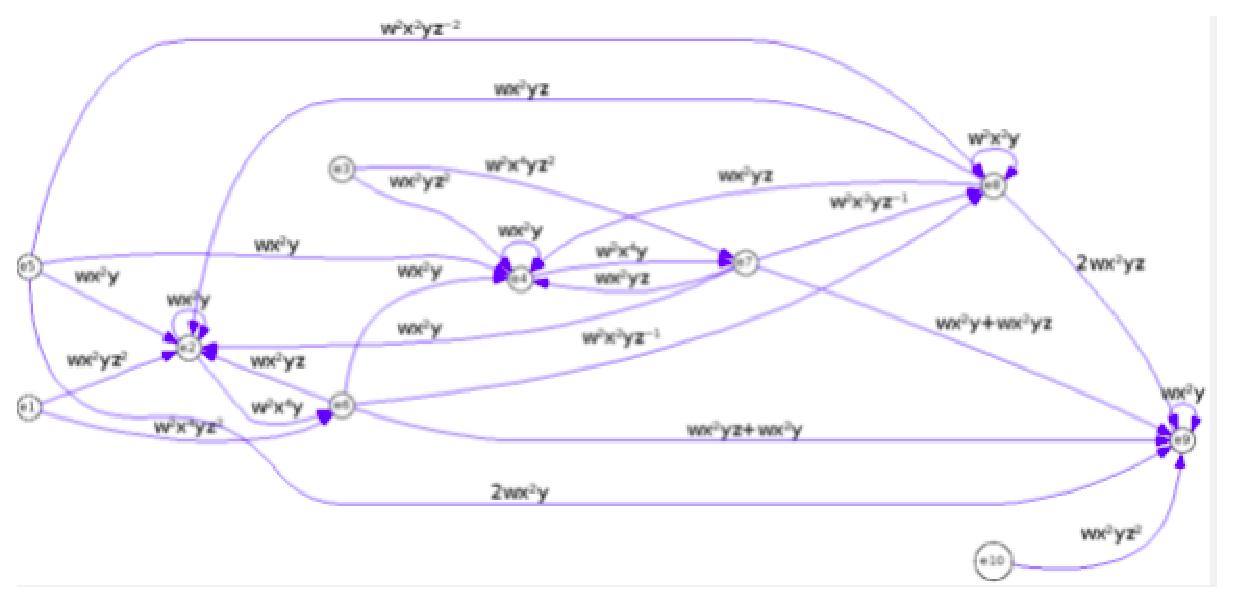
\includegraphics[width=15cm,height=10cm]{A2F2.eps}
%\begin{figure}[!htb]
\begin{minipage}[c]{.01\linewidth}
 \centering
 
 \end{minipage}
 \begin{minipage}[c]{.40\linewidth}
 \centering
 \begin{tikzpicture}[shorten >=1pt,node distance=3cm,initial text=,auto]
  \tikzstyle{every state}=[fill={rgb:black,1;white,10}]
  \node[state,initial]   (e_1)                       {$e_1$};
  \node[state,initial]           (e_5) [above of=e_1] {$e_5$};
   \node[state,initial]           (e_3) [above of=e_5]  {$e_3$};
  \node[state]           (e_4) [right of=e_5] {$e_4$};
  \node[state]           (e_2) [below right of= e_5]     {$e_2$};
  \node[state,accepting] (e_6) [ below right of=e_2]  {$e_6$};
  \node[state,accepting] (e_7) [right of= e_4]  {$e_7$};
  \node[state,accepting] (e_8) [above right of= e_7]  {$e_8$};
  \node[state,accepting] (e_9) [below right of=e_8]  {$e_9$};
  \node[state]           (e_{10}) [below of= e_9]     {$e_{10}$};

  \path[->]
  (e_1)   edge              node {$T_{1,2}$} (e_2)
        edge              node {$T_{1,6}$} (e_6)
  (e_2)  edge              node {$T_{2,6}$} (e_6)
   (e_3)     edge  [bend right] node {$T_{3,4}$} (e_4)
        edge  [bend left]     node {$T_{3,7}$} (e_7)
        
  (e_4) edge [loop above]  node {$T_{4,4}$} (   )
  (e_8) edge [loop right]  node {$T_{8,8}$} (   )
  (e_9) edge [loop right]  node {$T_{9,9}$} (   )
  (e_2) edge [loop above]  node {$T_{2,2}$} (   )
  (e_4)     edge [bend left]  node {$T_{4,7}$} (e_7)
   (e_5)     edge              node {$T_{5,2}$} (e_2)
             edge              node {$T_{5,4}$} (e_4)
             edge [bend left]             node {$T_{5,8}$} (e_8)
             edge [bend right]  node {$T_{5,9}$} (e_9)
    (e_6)    edge [bend left]  node {$T_{6,2}$} (e_2)
             edge [bend right] node {$T_{6,8}$} (e_8)
             edge [bend right]  node {$T_{6,4}$} (e_4)
             edge [bend right]  node {$T_{6,9}$} (e_9)
   (e_7)    edge [bend left]  node {$T_{7,2}$} (e_2)
            edge [bend left]  node {$T_{7,4}$} (e_4)
            edge [bend left]  node {$T_{7,8}$} (e_8)
            edge [bend left]  node {$T_{7,9}$} (e_9)
   (e_8)    edge [bend left]  node {$T_{8,2}$} (e_2)
            edge [bend right]  node {$T_{8,4}$} (e_4)
            edge [bend left]  node {$T_{8,9}$} (e_9)
   (e_{10}) edge [bend right]  node {$T_{10,9}$} (e_9);
\end{tikzpicture}
\end{minipage}
\caption{\label{Atfig12} Automate $\mathcal{A}_{2}$.}
\end{figure}
%\end{figure} 
\begin{spacing}{0.30}
\subsection*{Les transitions impossibles et les raisons pour lesquelles elles le sont}
\end{spacing}
\begin{spacing}{0.30}
\subsubsection*{Compte tenu de la proposition \ref{prop1} (perte de la connexité)}
\end{spacing}
$e_{1}\rightarrow e_{3}$, $e_{2}\rightarrow e_{3}$, $e_{3}\rightarrow e_{1}$, $e_{3}\rightarrow e_{2}$, $e_{1}\rightarrow e_{4}$, $e_{2}\rightarrow e_{4}$, $e_{4}\rightarrow e_{1}$ et $e_{4}\rightarrow e_{2}$.
\begin{spacing}{0.30}
\subsubsection*{Compte tenu de la proposition \ref{propdec191}}
\end{spacing}
$e_{1}\rightarrow e_{1}$, $e_{2}\rightarrow e_{1}$, $e_{5}\rightarrow e_{1}$, $e_{6}\rightarrow e_{1}$, $e_{7}\rightarrow e_{1}$, $e_{8}\rightarrow e_{1}$, $e_{3}\rightarrow e_{3}$, $e_{4}\rightarrow e_{3}$, $e_{5}\rightarrow e_{3}$, $e_{6}\rightarrow e_{3}$, $e_{7}\rightarrow e_{3}$, $e_{8}\rightarrow e_{3}$, $e_{1}\rightarrow e_{5}$, $e_{2}\rightarrow e_{5}$, $e_{3}\rightarrow e_{5}$, $e_{4}\rightarrow e_{5}$, $e_{5}\rightarrow e_{5}$, $e_{6}\rightarrow e_{5}$, $e_{7}\rightarrow e_{5}$, $e_{8}\rightarrow e_{5}$, $e_{3}\rightarrow e_{6}$, $e_{4}\rightarrow e_{6}$, $e_{5}\rightarrow e_{6}$, $e_{6}\rightarrow e_{6}$, $e_{7}\rightarrow e_{6}$, $e_{8}\rightarrow e_{6}$, $e_{1}\rightarrow e_{7}$, $e_{2}\rightarrow e_{7}$, $e_{5}\rightarrow e_{7}$, $e_{6}\rightarrow e_{7}$, $e_{7}\rightarrow e_{7}$, $e_{8}\rightarrow e_{7}$, $e_{1}\rightarrow e_{8}$, $e_{2}\rightarrow e_{8}$, $e_{3}\rightarrow e_{8}$, $e_{4}\rightarrow e_{8}$, $e_{9}\rightarrow e_{10}$ et $e_{2}\rightarrow e_{10}$.
\begin{spacing}{0.30}
\subsubsection*{Compte tenu de la proposition \ref{prop2606221}}
\end{spacing}
$e_{1}\rightarrow e_{9}$, $e_{2}\rightarrow e_{9}$, $e_{3}\rightarrow e_{9}$ et $e_{4}\rightarrow e_{9}$.
\begin{spacing}{0.30}
\subsubsection*{Compte tenu des propositions \ref{prop2606221} et \ref{propdec191}}
\end{spacing}
$e_{1}\rightarrow e_{10}$, $e_{2}\rightarrow e_{10}$, $e_{3}\rightarrow e_{10}$ et $e_{4}\rightarrow e_{10}$.
\begin{spacing}{0.30}
\subsubsection*{Compte tenu des propositions \ref{prop3} et \ref{propdec191}}
\end{spacing}
$e_{9}\rightarrow e_{1}$, $e_{9}\rightarrow e_{2}$, $e_{9}\rightarrow e_{3}$, $e_{9}\rightarrow e_{4}$,   $e_{9}\rightarrow e_{5}$, $e_{9}\rightarrow e_{6}$, $e_{9}\rightarrow e_{7}$, $e_{9}\rightarrow e_{8}$, $e_{10}\rightarrow e_{1}$, $e_{10}\rightarrow e_{2}$, $e_{10}\rightarrow e_{3}$, $e_{10}\rightarrow e_{4}$, $e_{10}\rightarrow e_{5}$, $e_{10}\rightarrow e_{6}$, $e_{10}\rightarrow e_{7}$ et $e_{10}\rightarrow e_{8}$.
\begin{spacing}{0.30}
\section{Automate $\mathcal{A}_{3}$}
\end{spacing}
$\mathcal{A}_{3}$ a $12$ classes d'états qui sont présentées ci-dessous.
\begin{eqnarray*}
& & cl_{1} = (100,\{\{0\}\}), \quad cl_{2} = (010,\{\{0\}\}), \quad cl_{3}=(001,\{\{0\}\}),\\
& &cl_{4}=(110,\{\{0\}\}),\quad cl_{5}=(101,\{\{0,1\}\}),\quad cl_{6} = (101,\{\{0\},\{1\}\}), \\
& &cl_{7} = (011,\{\{0\}\}),\quad cl_{8}=(111,\{\{0\}\}),\quad cl_{9}=(10,\{\{0\}\}),\\
& & cl_{10}=(01,\{\{0\}\}),\quad cl_{11} =(11,\{\{0\}\})\textit{ et }\quad cl_{12}=(1,\{\{0\}\}).
\end{eqnarray*} 
On a donc les états suivants
\small
\begin{longtable}{|c|c|c|} 
\hline
$e_{1}=(100,000,\{\{0\}\})$&
$e_{2}=(100,100,\{\{0\}\})$&
$e_{3}=(010,000,\{\{0\}\})$\\
$e_{4}=(010,010)\{\{0\}\})$&
$e_{5}=(001,000,\{\{0\}\}$&
$e_{6}=(001,001,\{\{0\}\})$\\
$e_{7}=(110,110,\{\{0\}\})$&
$e_{8}=(110,210,\{\{0\}\})$&
$e_{9}=(110,120,\{\{0\}\})$\\
$e_{10}=(110,220,\{\{0\})$&
$e_{11}=(101,000,\{\{0\},\{1\}\})$& 
$e_{12}=(101,101,\{\{0\},\{1\}\})$ \\
$e_{13}=(101,100,\{\{0\},\{1\}\})$& 
$e_{14}=(101,001,\{\{0\},\{1\})$&
$e_{15}=(101,101,\{\{0,1\}\})$ \\
$e_{16}=(011,011,\{\{0\}\})$&
$e_{17}=(011,021,\{\{0\}\})$&
$e_{18}=(011,012,\{\{0\}\})$\\
$e_{19}=(011,022,\{\{0\}\})$&
$e_{20}=(111,121,\{\{0\}\})$&
$e_{21}=(111,221,\{\{0\}\})$\\
$e_{22}=(111,122,\{\{0\}\})$&
$e_{23}=(111,222,\{\{0\}\})$&
$e_{24}=(111,131,\{\{0\}\})$\\
$e_{25}=(111,231,\{\{0\}\})$&
$e_{26}=(111,132,\{\{0\}\})$&
$e_{27}=(111,232,\{\{0\}\})$\\
$e_{28}=(10,00,\{\{0\}\})$&
$e_{29}=(10,10,\{\{0\}\})$&
$e_{30}=(01,00,\{\{0\}\})$\\
$e_{31}=(01,01,\{\{0\}\})$&
$e_{32}=(11,11,\{\{0\}\})$&
$e_{33}=(11,21,\{\{0\}\})$\\
$e_{34}=(11,12,\{\{0\}\})$&
$e_{35}=(11,22,\{\{0\}\})$&
$e_{36}=(1,0,\{\{0\}\})$ \\
$e_{37}=(1,1,\{\{0\}\})$ & &\\
\hline
\caption{\label{tab6} Les états de $\mathcal{A}_{3}$.}
\end{longtable}
\normalsize
 
 Les transitions possibles sont les suivantes:
 \small
\begin{longtable}{|c|c|} 
\hline
$T_{1,2}= yz^2wx^2$\quad\quad \quad &

$T_{1,8}= yz^2w^2x^4$\\

$T_{1,13}= yz^2w^2x^6$ &

$T_{1,21}= yz^2w^3x^6$\\

$T_{2,2}= ywx^2$&

$T_{2,8}= yw^2x^4$\\

$T_{2,13}= yw^2x^6$&

$T_{2,21}= yw^3x^6$\\

$T_{3,4}= yz^2wx^2$&

$T_{3,9}= yz^2w^2x^4$\\

$T_{3,17}= yz^2w^2x^4$&

$T_{3,24}= yz^3w^3x^6$\\

$T_{4,4}= ywx^2$&

$T_{4,9}= yw^2x^4$\\

$T_{4,17}= yw^2x^4$&

$T_{4,24}= yzw^3x^6$\\

$T_{5,6}= yz^2wx^2$&

$T_{5,14}= yz^2w^2x^6$\\

$T_{5,18}= yz^2w^2x^4$&

$T_{5,22}= yz^2w^3x^6$\\

$T_{6,6}= ywx^2$&

$T_{6,14}= yw^2x^6$\\

$T_{6,18}= yw^2x^4$&

$T_{6,22}= yw^3x^6$\\

$T_{7,2}= ywx^2$&

$T_{7,4}= ywx^2$\\

$T_{7,10}= yz^{-2}w^2x^2$&

$T_{7,13}= yw^2x^6$\\

$T_{7,17}= yw^2x^4$&

$T_{7,25}= yz^{-1}w^3x^4$\\

$T_{7,29}= ywx^2$&

$T_{7,33}= yw^2x^4$\\

$T_{8,2}= yzwx^2$&

$T_{8,4}= ywx^2$\\

$T_{8,10}= yz^{-1}w^2x^2$&

$T_{8,13}= yzw^2x^6$\\

$T_{8,17}= yw^2x^4$&

$T_{8,25}= yw^3x^4$\\

$T_{8,29}= ywx^2$&

$T_{8,33}= yw^2x^4$\\

$T_{9,2}= ywx^2$&

$T_{9,4}= yzwx^2$\\

$T_{9,10}= yz^{-1}w^2x^2$&

$T_{9,13}= yw^2x^6$\\

$T_{9,17}= yzw^2x^4$&

$T_{9,25}= yw^3x^4$\\

$T_{9,29}= yzwx^2$&

$T_{9,33}= yzw^2x^4$\\

$T_{10,2}= yzwx^2$&

$T_{10,4}= yzwx^2$\\

$T_{10,10}= yw^2x^2$ &

$T_{10,13}= yzw^2x^6$\\

$T_{10,17}= yzw^2x^4$&

$T_{10,25}= yzw^3x^4$\\

$T_{10,29}= yzwx^2$&

$T_{10,33}= yzw^2x^4$\\

$T_{11,12}= yz^4w^2x^4$&

$T_{11,23}= yz^2w^3x^4$\\

$T_{12,12}= yw^2x^4$&

$T_{12,23}= yz^{-2}w^3x^4$\\
 
$T_{13,12}= yz^2w^2x^4$& 

$T_{13,23}= yzw^3x^4$\\

$T_{14,12}= yz^2w^2x^4$ &

$T_{14,23}= yw^3x^4$\\

$T_{15,2}= ywx^2$&

$T_{15,6}= ywx^2$\\

$T_{15,8}= yw^2x^4$&

$T_{15,15}= yw^2x^4$\\

$T_{15,18}= yw^2x^4$ &

$T_{15,23}= yz^{-2}w^3x^4$\\

$T_{15,29}= ywx^2$&

$T_{15,31}= ywx^2$\\

$T_{15,33}= yw^2x^4$&

$T_{15,34}= yw^2x^4$\\

$T_{15,37}= 2ywx^2$&

$T_{16,4}= ywx^2$\\

$T_{16,6}= ywx^2$ &

$T_{16,9}= yw^2x^4$\\

$T_{16,14}= yw^2x^6$&

$T_{16,19}= yz^{-2}w^2x^2$\\

$T_{16,26}= yz^{-1}w^3x^4$\quad\quad \quad &

$T_{16,31}= ywx^2$\\

$T_{16,34}= yw^2x^4$&

$T_{17,4}= yzwx^2$\\

$T_{17,6}= ywx^2$&

$T_{17,9}= yzw^2x^4$\\

$T_{17,14}= yw^2x^6$&

$T_{17,19}= yz^{-1}w^2x^2$\\

$T_{17,26}= yw^3x^4$&

$T_{17,31}= yzwx^2$ \\

$T_{17,34}= yzw^2x^4$&

$T_{18,4}= ywx^2$\\

$T_{18,6}= yzwx^2$&

$T_{18,9}= yw^2x^4$\\

$T_{18,14}= yzw^2x^6$&

$T_{18,19}= yz^{-1}w^2x^2$\\

$T_{18,26}= yw^3x^4$&

$T_{18,31}= ywx^2$\\

$T_{18,34}= yw^2x^4$&

$T_{19,4}= yzwx^2$\\

$T_{19,6}= yzwx^2$&

$T_{19,9}= yzw^2x^4$\\

$T_{19,14}= yzw^2x^6$&

$T_{19,19}= yw^2x^2$\\

$T_{19,26}= yzw^3x^4$&

$T_{19,31}= yzwx^2$\\

$T_{19,34}= yzw^2x^4$&

$T_{20,2}= ywx^2$\\

$T_{20,4}= yzwx^2$&

$T_{20,6}= ywx^2$\\

$T_{20,10}= yz^{-1}w^2x^2$&

$T_{20,15}= yw^2x^4$\\

$T_{20,19}= yz^{-1}w^2x^2$&

$T_{20,27}= yz^{-2}w^3x^2$\\

$T_{20,29}= yzwx^2+ywx^2$&

$T_{20,31}= yzwx^2+ywx^2$\\

$T_{20,35}= 2yz^{-1}w^2x^2$ &

$T_{20,37}= 2yw^2x^2+yz^{-1}w^2x^2$\\

$T_{21,2}= yzwx^2$&

$T_{21,4}= yzwx^2$ \\
$T_{21,6}= ywx^2$&

$T_{21,10}= yw^2x^2$ \\

$T_{21,15}= yzw^2x^4$ &

$T_{21,19}= yz^{-1}w^2x^2$\\

$T_{21,27}= yz^{-1}w^3x^2$ &

$T_{21,31}= yzwx^2+ywx^2$\\ 
$T_{21,29}= 2yzwx^2$ &

$T_{21,35}= yw^2x^2+yz^{-1}w^2x^2$\\

$T_{21,37}= 2yzwx^2+ywx^2$ &

$T_{22,2}= ywx^2$\\

$T_{22,4}= yzwx^2$&

$T_{22,6}= yzwx^2$ \\

$T_{22,10}= yz^{-1}w^2x^2$&

$T_{22,15}= yzw^2x^4$\\

$T_{22,19}= yw^2x^2$&

$T_{22,27}= yz^{-1}w^3x^2$\\

$T_{22,29}= yzwx^2+ywx^2$& 

$T_{22,31}= 2yzwx^2$ \\

$T_{22,35}= yw^2x^2+yz^{-1}w^2x^2$ &

$T_{22,37}= 2yzwx^2+ywx^2$\\

$T_{23,2}= yzwx^2$ &

$T_{23,4}= yzwx^2$\\

$T_{23,6}= yzwx^2$&

$T_{23,10}= yw^2x^2$ \\

$T_{23,15}= yz^2w^2x^4$&

$T_{23,19}= yw^2x^2$\\

$T_{23,27}= yw^3x^2$&

$T_{23,29}= 2yzwx^2$\\

$T_{23,31}= 2yzwx^2$&

$T_{23,35}= 2yw^2x^2$\\

$T_{23,37}= 3yzwx^2$&

$T_{24,2}= ywx^2$\\

$T_{24,4}= yzwx^2$&

$T_{24,6}= ywx^2$\\

$T_{24,10}= yz^{-1}w^2x^2$&

$T_{24,15}= yw^2x^4$ \\

$T_{24,19}= yz^{-1}w^2x^2$&

$T_{24,27}= yz^{-2}w^3x^2$\\ 

$T_{24,29}= yzwx^2+ywx^2$ &

$T_{24,31}= yzwx^2+ywx^2$\\ 

$T_{24,35}= 2yz^{-1}w^2x^2$&

$T_{24,37}= yzwx^2+2ywx^2$ \\

$T_{25,2}= yzwx^2$&

$T_{25,4}= yzwx^2$\\

$T_{25,6}= ywx^2$&

$T_{25,10}= yw^2x^2$\\

$T_{25,15}= yzw^2x^4$&

$T_{25,19}= yz^{-1}w^2x^2$\\

$T_{25,27}= yz^{-1}w^3x^2$&

$T_{25,29}= 2yzwx^2$\\

$T_{25,31}= yzwx^2+ywx^2$ & 

$T_{25,35}= yw^2x^2+yz^{-1}w^2x^2$\\

$T_{25,37}= 2yzwx^2+ywx^2$& 

$T_{26,2}= ywx^2$ \\

$T_{26,4}= yzwx^2$&

$T_{26,6}= yzwx^2$ \\

$T_{26,10}= yz^{-1}w^2x^2$ &

$T_{26,15}= yzw^2x^4$\\ 

$T_{26,19}= yw^2x^2$ &

$T_{26,27}= yz^{-1}w^3x^2$ \\

$T_{26,29}= yzwx^2+ywx^2$&

$T_{26,31}= 2yzwx^2$\\

$T_{26,35}= yw^2x^2+yz^{-1}w^2x^2$&

$T_{26,37}= 2yzwx^2+ywx^2$\\

$T_{27,2}= yzwx^2$&

$T_{27,4}= yzwx^2$\\

$T_{27,6}= yzwx^2$&

$T_{27,10}= yw^2x^2$\\

$T_{27,15}= yz^2w^2x^4$&

$T_{27,19}= yw^2x^2$\\

$T_{27,27}= yw^3x^2$&

$T_{27,29}= 2yzwx^2$\\

$T_{27,31}= 2yzwx^2$&

$T_{27,35}= 2yw^2x^2$\\

$T_{27,37}= 3yzwx^2$&

$T_{28,29}= yz^2wx^2$\\

$T_{28,33}= yz^2w^2x^4$&

$T_{29,29}= ywx^2$\\

$T_{29,33}= yw^2x^4$&

$T_{30,31}= yz^2wx^2$\\

$T_{30,34}= yz^2w^2x^4$&

$T_{31,31}= ywx^2$\\

$T_{31,34}= yw^2x^4$&

$T_{32,29}= ywx^2$\\

$T_{32,31}= ywx^2$&

$T_{32,35}= yz^{-2}w^2x^2$\\

$T_{32,37}= 2ywx^2$&

$T_{33,29}= yzwx^2$\\

$T_{33,31}= ywx^2$&

$T_{33,35}= yz^{-1}w^2x^2$\\

$T_{33,37}= yzwx^2+ywx^2$&

$T_{34,29}= ywx^2$\\

$T_{34,31}= yzwx^2$&

$T_{34,35}= yz^{-1}w^2x^2$\\

$T_{34,37}= yzwx^2+ywx^2$&

$T_{35,29}= yzwx^2$\\

$T_{35,31}= yzwx^2$&

$T_{35,35}= yw^2x^2$\\

$T_{35,37}= 2yzwx^2$&

$T_{36,37}= yz^2wx^2$\\

$T_{37,37}= ywx^2$& \\
\hline
\caption{\label{tab3} Les transitions possibles de $\mathcal{A}_{3}$.}
\end{longtable} 
\normalsize
Les états initiaux de $\mathcal{A}_{3}$ sont $e_{1}$, $e_{3}$, $e_{5}$, $e_{7}$, $e_{11}$, $e_{16}$,  $e_{20}$.  Ses états finaux  sont $e_{15}$, $e_{21}$, $e_{22}$, $e_{23}$, $e_{24}$, $e_{25}$,  $e_{26}$, $e_{27}$, $e_{33}$, $e_{34}$, $e_{35}$, $e_{37}$.       
\section{Validation des valeurs dans les matrices de transfert $\mathcal{M}_{2}$ et $\mathcal{M}_{3}$}
Dans cette section nous vérifions si les entrées des matrices $\mathcal{M}_{2}$ et $\mathcal{M}_{3}$ sont fiables, c'est-à-dire si la somme des coefficients des entrées $a_{i,j}$  de la  matrice $\mathcal{M}_{2}^{n}$ ( ou  $\mathcal{M}_{3}^{n}$), où $n$ est un entier naturel supérieur ou égal à $0$, correspond à la $(n+1)^{ieme}$ valeur de  la suite du nombre de polyominos inscrits dans le rectangle de type $2$ (ou de type $3$) sur  \emph{The On-Line Encyclopedia of Integer Sequences} \citep{Oeis,Oeis2}. Pour cela, nous calculons la matrice $M_{2}^{n}$ (respectivement $M_{3}^{n}$) et comparons la somme $S_{n}$ des coefficients des polynômes correspondants aux entrées $a_{i,j}$ de cette dernière. On note que $a_{i,j}$ est une transition de  l'état initial $e_{i}$ à l'état final  $e_{j}$.
\subsection{Validation des valeurs de la matrice $\mathcal{M}_{2}$}
\begin{itemize}
\item[(i)] Cas $n=0$

Dans ce cas particulier, il s'agit de trouver l'unique polyomino inscrit dans le rectangle de base $B=2$ et de hauteur $1$ (voir figure \ref{uni2}). La valeur de $S_{0}$ vaut particulièrement $1$ dans ce cas.
 \begin{figure}[!htb]
 \begin{minipage}[c]{.26\linewidth}
  \centering
  \end{minipage}
  \hfill
\begin{minipage}[c]{.56\linewidth}
  \centering
\begin{logicpuzzle}[rows=1,columns=2,color=cyan!100, width=750px,scale=0.5]
\fillcell{1}{1}
\fillcell{2}{1}
\framepuzzle[black!50]
\end{logicpuzzle}
\end{minipage}
\caption{\label{uni2} Polyomino inscrit dans le rectangle $2\times 1$.}
\end{figure}
\item[(ii)] Cas $n=1$

Il suffit, dans ce cas, de faire la somme $S_{1}$ des coefficients des polynômes de Laurent des entrées $m_{i,j}$ de la matrice $\mathcal{M}_{2}$  correspondantes aux transitions des états initiaux aux états finaux. Dans le tableau ci-dessous, nous listons les entrées  non nulles correspondantes aux transitions d'états initiaux aux états finaux.\\

\begin{tabular}{|c|c|c|c|}
 \hline
  Transition& $m_{i,j}$ & Somme  coefficients\\
 \hline
 $e_{1}\rightarrow e_{6}$ & $w^{2}x^{4}yz^{2}$ & $1$ \\
 \hline
 $e_{3}\rightarrow e_{7}$ & $w^{2}x^{4}yz^{2}$ & $1$ \\
 \hline
 $e_{5}\rightarrow e_{8}$ & $w^{2}x^{2}yz^{-2}$ & $1$ \\
 \hline
 $e_{5}\rightarrow e_{9}$ & $2wx^{2}y$ & $2$ \\
 \hline
\end{tabular}
\mbox{ }\\
$S_{1}=1+1+1+2=5$. Ce qui signifie qu'on a au total $5$ polyominos inscrits dans le carré $2\times 2$.
\item[(iii)] Cas $n=2$

 Nous faisons la  somme $S_{2}$ des coefficients des polynômes de Laurent des entrées $m_{i,j}$ de la matrice $\mathcal{M}_{2}^{2}$  correspondantes aux transitions des états initiaux aux états finaux.
 
 \begin{tabular}{|c|c|c|c|}
 \hline
  Transition & $m_{i,j}$&Somme  coefficients\\
 \hline
  $e_{1}\rightarrow e_{6}$ & $w^3x^6y^2z^{2}$ &$1$ \\ 
 \hline
 $e_{1}\rightarrow e_{8}$ & $w^4x^6y^2z$  & $1$ \\
 \hline
 $e_{1}\rightarrow e_{9}$ & $w^3x^6y^2z^{3}+w^3x^6y^2z^{2}$ & $2$ \\
 \hline
 $e_{3}\rightarrow e_{7}$ & $w^3x^6y^2z^{2}$ & $1$ \\
 \hline
 $e_{3}\rightarrow e_{8}$ & $ w^4x^6y^2z$ & $1$ \\
 \hline
 $e_{3}\rightarrow e_{9}$ & $w^3x^6y^2z^{3}+w^3x^6y^2z^{2} $\ & $2$ \\
 \hline
  $e_{5}\rightarrow e_{6}$&$ w^3x^6y^2 $& $1$\\
 \hline
  $e_{5}\rightarrow e_{7}$&$ w^3x^6y^2, $& $1$\\
 \hline
  $e_{5}\rightarrow e_{8}$&$ w^4x^4y^2z^{-2}  $& $1$\\
 \hline
  $e_{5}\rightarrow e_{9}$&$2w^3x^4y^2z^{-1}+2w^2x^4y^2$& $4$\\
 \hline
\end{tabular}
\mbox{ }\\\\
$S_{2}=1+1+2+1+1+2+1+1+1+4=15$.

\item[(iv)] Cas $n=3$\\
 Nous listons les entrées $m_{i,j}$ non nulles, $i\in\{1,3,5\}$ et $j\in\{6,7,8,9\}$. 
 On a 
 
$m_{1,6}=w^4x^8y^3z^2+w^5x^{10}y^3z^3$,  $m_{1,7}=w^5x^{10}y^3z^2 $,  $m_{1,8}=w^5x^8y^3z+w^6x^8y^3z$,  $m_{1,9}=2w^5x^8y^3z^2+2w^4x^8y^3z^3+2w^4x^8y^3z^2$,
$m_{3,6}=w^5x^{10}y^3z^2$, $m_{3,7}=w^4x^8y^3z^2+w^5x^{10}y^3z^3 $,  $m_{3,8}=w^5x^8y^3z+w^6x^8y^3z$,  $m_{3,9}=2w^5x^8y^3z^2+2w^4x^8y^3z^3+2w^4x^8y^3z^2$, 
$m_{5,6}=w^4x^8y^3+w^5x^8y^3z^{-1}$, $m_{5,7}=w^4x^8y^3+w^5x^8y^3z^{-1}$,$m_{5,8}=2w^5x^8y^3z^{-1}+w^6x^6y^3z^{-2}$, $m_{5,9}=2w^3x^6y^3+2w^4x^6y^3z^{-1}+2w^4x^8y^3+2w^4x^8y^3z+2w^5x^6y^3z^{-1}$.

$S_{3}=2+1+2+6+1+2+2+6+2+2+3+10=39$.

\item[(v)] Cas $n=4$\\

$m_{1,6}=w^7x^{12}y^4z^{2}+2w^6x^{12}y^4z^{3}+w^5x^{10}y^4z^{2}$, $m_{1,7}=w^7x^{12}y^4z^{2}+2z^2w^6x^{12}y^4$, $m_{1,8}=w^7x^{12}y^4z^2+w^7x^{10}y^4z+w^8x^{10}y^4z+w^7x^{12}y^4z+w^6x^{10}y^4z$, $m_{1,9}=2z^2w^7x^{10}y^4+2z^3w^6x^{12}y^4+w^6x^{12}y^4z^{2}+4z^2w^6x^{10}y^4+3z^2w^5x^{10}y^4+w^6x^{12}y^4z^{3}+3w^5x^{10}y^4z^{3}$,  $m_{3,6}=w^7x^{12}y^4z^{2}+2w^6x^{12}y^4z^{2}$, $m_{3,7}=w^7x^{12}y^4z^{2}+2z^3w^6x^{12}y^4+z^2w^5x^{10}y^4$, $m_{3,8}=w^7x^{12}y^4z^{2}+w^7x^{10}y^4z+w^8x^{10}y^4z+w^7x^{12}y^4z+w^6x^{10}y^4z$, $m_{3,9}=2w^7x^{10}y^4z^{2}+2w^6x^{12}y^4z^{3}+w^6x^{12}y^4z^{2}+4z^2w^6x^{10}y^4+3w^5x^{10}y^4z^{2}+w^6x^{12}y^4z^{4}+3w^5x^{10}y^4z^{3}$, $m_{5,6}=w^6x^{12}y^4+w^5x^{10}y^4+w^7x^{10}y^4z^{-1}+w^6x^{12}y^4z+w^6x^{10}y^4z^{-1}$, $m_{5,7}=w^6x^{12}y^4+w^5x^{10}y^4+w^7x^{10}y^4z^{-1}+w^6x^{12}y^4z+w^6x^{10}y^4z^{-1}$,  $m_{5,8}=
2w^7x^{10}y^4z^{-2}+2w^7x^{10}y^4z^{-1}+w^8x^8y^4z^{-2}+2w^6x^{10}y^4z^{-1}$, $m_{5,9}= 2w^6x^8y^4z^{-1}+4w^5x^{10}y^4z+2w^4x^8y^4+6w^6x^{10}y^4+2w^7x^8y^4z^{-1}+4w^5x^{10}y^4z^{-1}+2w^5x^8y^4z^{-1}+2w^6x^{10}y^4z^{-1}$.
\mbox{ }\\\\
$S_{4}=4+3+5+16+3+4+5+16+5+5+7+24=97$.
\item[(vi)] Cas $n=5$\\

Pour ce cas, étant donné que les expressions des entrées $m_{i,j}$ de la matrice $\mathcal{M}_{2}^{5}$ sont de très grandes tailles, pour chacune d'elles, nous donnons la somme des coefficients  de ses monômes.\\\\
 \tiny
\begin{tabular}{|c|c|c|c|c|c|c|c|c|c|c|c|c|}
 \hline
Entrées & $m_{1,6}$& $m_{1,7}$&$m_{1,8}$ & $m_{1,9}$& $m_{3,6}$ &$m_{3,7}$ & $m_{3,8}$&$m_{3,9}$ & $m_{5,6}$& $m_{5,7}$ &$m_{5,8}$ &$m_{5,9}$ \\
 \hline
 coef  &$9$ &$8$&$12$ &$40$  &$8$ &$9$ &$12$  &$40$&$12$ &$12$  &$17$&$58$ \\
 \hline
 \end{tabular}
 \normalsize
\mbox{ }\\\\
$S_{5}=9+8+12+40+8+9+12+40+12+12+17+58=237$.
\end{itemize}
Dans le tableau \ref{v2} nous listons, pour chaque valeur $n$, $1\leq n\leq 15$, le nombre  polyominos inscrits dans le rectangle de base $2$ et de hauteur $H=n+1$. Pour chaque valeur $n$, $s_{1}$, $s_{2}$ et $s_{5}$ désigne respectivement les nombres de polyominos obtenus à partir des états initiaux $e_{1}$, $e_{3}$ et $e_{5}$ tandis-que $S_{n}$ est le nombre total de polyominos inscrits dans le rectangle $2\times (n+1)$.
\begin{small}
\begin{longtable}{|c|c|c|c|c|c|c|c|c|c|c|} 
\hline
$n$&$s_{1}$&$s_{3}$&$s_{5}$&$S_{n}$\\
\hline
$1$& $ 1 $&  $1 $& $ 2$&$ 5$\\
\hline
$2$& $ 4$& $ 4$& $ 7$&$15 $\\
\hline
$3$& $11 $& $11 $& $17 $&$39 $\\
\hline39
$4$& $ 28$& $28 $& $ 41$&$ 97$\\
\hline
$5$& $69 $& $69 $& $99 $&$237 $\\
\hline
$6$& $168$& $168$& $279$&$575$\\
\hline
$7$&$407$ &$407$ &$577$ &$1391$\\
\hline
$8$&$984$ & $984$&$1393$ &$ 3361
$\\
\hline
$9$& $2377$& $2377$&$3363$ &$8117$\\
\hline
$10$&$5740$ &$5740$ & $8119$&$19599$\\
\hline
$11$& $13859$&$13859$ & $19601$&$47319$\\
\hline
$12$&$33460$ & $33460$& $47321$&$114241$\\
\hline
$13$&$80781$ & $80781$& $114243$&$275805
$\\
\hline
$14$&$195024$ & $195024$&$275807$ &$665855$\\
\hline
$15$& $470831$&$470831$& $665857$&$1607519$\\
\hline
\caption{\label{v2} Nombres de polyominos inscrits dans quelques rectangles de type $2$.}
\end{longtable}
\end{small}
À travers les quinze cas présentés  ci-dessus, nous avons obtenu les quinze premières valeurs de la suite numéro $A034182 $ des nombres de polyominos inscrits dans un rectangle de base $2$ du site \emph{OEIS}. Sur la base de ces résultats, nous conjecturons que pour toute valeur de $n\geq 5$, la $(n+1)^{ieme}$ valeur de la suite des nombres de polyominos inscrits dans un rectangle de largeur $2$ est la même que celle de \emph{OEIS}.
\begin{spacing}{0.30}
\subsection{Validation des valeurs de la matrice $\mathcal{M}_{3}$}
\end{spacing}
Tout comme la section précédente, nous calculons, en utilisant les puissances de la matrice $\mathcal{M}_{3}$, les sept premières valeurs de la suite des nombres de polyominos inscrits dans un rectangle du type $3$ tout en les comparant à celles de l'\emph{OEIS}. On rappelle que  l'automate $\mathcal{A}_{3 }$ a pour   états  initiaux les états $e_{1}, e_{3}, e_{5}, e_{7}, e_{11}, e_{16}, e_{20}$ et pour états finaux les états $e_{15},  e_{21}, e_{22}, e_{23}, e_{24}, e_{25}$, $ e_{26}, e_{27}, e_{33}, e_{34},  e_{35},  e_{37}. $

Pour chaque état initial $e_{i}$ de $\mathcal{A}_{3}$, nous calculons la somme $s_{i}$ des coefficients de toutes les entrées $m_{i,j}$ de la matrice $\mathcal{M}_{3}^{n}$, correspondantes aux suites de transitions de $e_{i}$ à $e_{j}$, $j\in \{15, 21, 22, 23, 24, 25, 26, 27, 33, 34, 35, 37\}$. On désigne par  $S_{n}$ la somme des $s_{i}$, $i$ parcourant l'ensemble des indices des états initiaux de $\mathcal{A}_{3}$.
\begin{itemize}
\item[(i)] Cas $n=0$
Dans ce cas particulier, il s'agit de trouver l'unique polyomino inscrit dans le rectangle de type $B=3$ et de hauteur $1$ (voir figure \ref{uni3}). La valeur de $S_{0}$ vaut particulièrement $1$ dans ce cas.
 \begin{figure}[!htb]
 \begin{minipage}[c]{.26\linewidth}
  \centering
  \end{minipage}
  \hfill
\begin{minipage}[c]{.56\linewidth}
  \centering
\begin{logicpuzzle}[rows=1,columns=3,color=cyan!100, width=750px,scale=0.5]
\fillcell{1}{1}
\fillcell{2}{1}
\fillcell{3}{1}
\framepuzzle[black!50]
\end{logicpuzzle}
\end{minipage}
\caption{\label{uni3} Polyomino inscrit dans le rectangle $3\times 1$.}
\end{figure}
\item[(ii)] Cas $n=1$ (matrice $\mathcal{M}_{3}$)\\

\begin{tabular}{|c|c|c|c|c|c|c|c|c|c|c|c|c|}
 \hline
 $i$ & $1$ & $3$ & $5$ & $7$ & $11$ & $16$ & $20$&$S_{1}$\\
 \hline
 $s_{i}$ & $1$ & $1$ & $1$ & $2$ & $1$&$1$&$8$&$15$\\
 \hline
 \end{tabular}
 \mbox{ }\\
\item[(iii)] Cas $n=2$ (matrice $\mathcal{M}_{3}^{2}$)\\
\begin{tabular}{|c|c|c|c|c|c|c|c|c|c|c|c|c|}
 \hline
 $i$ & $1$ & $3$ & $5$ & $7$ & $11$ & $16$ & $20$&$S_{2}$\\
 \hline
 $s_{i}$ & $11$ & $12$ & $12$ & $18$ & $8$&$17$&$33$&$111$\\
 \hline
 \end{tabular}
 \mbox{ }\\
\item[(iv)] Cas $n=3$ (matrice $\mathcal{M}_{3}^{3}$)\\
\mbox{}\\
\begin{tabular}{|c|c|c|c|c|c|c|c|c|c|c|c|c|}
 \hline
 $i$ & $1$ & $3$ & $5$ & $7$ & $11$ & $16$ & $20$&$S_{3}$\\
 \hline
 $s_{i}$ & $70$ & $77$ & $74$ & $110$ & $41$&$111$&$166$&$749$\\
 \hline
 \end{tabular}
 \mbox{ }\\
\item[(v)] Cas $n=4$ (matrice $\mathcal{M}_{3}^{4}$)\\
\mbox{}\\
\begin{tabular}{|c|c|c|c|c|c|c|c|c|c|c|c|c|}
 \hline
 $i$ & $1$ & $3$ & $5$ & $7$ & $11$ & $16$ & $20$&$S_{4}$\\
 \hline
 $s_{i}$ & $387$ & $468$ & $387$ & $607$ & $206$&$607$&$833$&$3495$\\
 \hline
 \end{tabular}
 \mbox{ }\\
\item[(vi)] Cas $n=5$ (matrice $\mathcal{M}_{3}^{5}$)\\
\mbox{}\\
\begin{tabular}{|c|c|c|c|c|c|c|c|c|c|c|c|c|}
 \hline
 $i$ & $1$ & $3$ & $5$ & $7$ & $11$ & $16$ & $20$&$S_{5}$\\
 \hline
 $s_{i}$ & $2033$ & $2515$ & $2033$ & $3177$ & $1039$&$3177$&$4215$&$18189$\\
 \hline
 \end{tabular}
 \mbox{ }\\
\item[(vii)] Cas $n=6$ (matrice $\mathcal{M}_{3}^{6}$)\\
 \mbox{ }\\
 \begin{tabular}{|c|c|c|c|c|c|c|c|c|c|c|c|c|}
 \hline
 $i$ & $1$ & $3$ & $5$ & $7$ & $11$ & $16$ & $20$&$S_{6}$\\
 \hline
 $s_{i}$ & $10464$ & $13084$ & $10464$ & $16324$ & $5254$&$16324$&$21317$&$93231$\\
 \hline
 \end{tabular}
\end{itemize}
\mbox{}\\\mbox{}\\
Dans le tableau \ref{v3} nous listons, pour chaque valeur $n$, $1\leq n\leq 11$, le nombre  polyominos inscrits dans le rectangle de base $3$ et de hauteur $H=n+1$.
\begin{tiny}
\begin{longtable}{|c|c|c|c|c|c|c|c|c|c|c|} 
\hline
n&$s_{1}$&$s_{3}$&$s_{5}$&$s_{7}$&$s_{11}$&$s_{16}$&$s_{20}$&$S_{n}$\\
\hline
$1$& 1
 & 1
& 1 & 2
& 1
& 1
& 8& 15\\

\hline
$2$& 11
 & 12
& 12 & 18
& 8 
& 17
& 33 & 111\\

\hline
$3$& 70
 & 81
& 70 & 111
& 41
& 111
& 165 & 649\\

\hline
$4$& 387
 & 468
& 387 & 607
& 206
& 607
& 833& 3495\\

\hline
$5$& 2033
 & 2515
& 2033 & 3177
& 1039
& 3177
&4215 &18189\\
\hline
$6$& 10464
 & 13084
& 10464& 16324
& 5254
&16324 &
21317 &93231  \\
\hline
$7$&53359
 & 67049
& 53359& 83174
& 26571
&83174
 &  10779&474479\\
\hline
$8$&270897
 &341190
 &270897
 &422104
 &134364
 & 422104&545065 &2406621
\\
\hline
$9$&  1372430
&1730463
 &1372430
 & 2138101
& 679429
& 2138101
&2756183
 &12187137
\\
\hline
$10$&6946143
 &8762848
 &6946143
 & 10820447
& 3435612
&10820447 & 13936969
& 61668609\\
\hline
$11$&35139171
 &44340711
 & 35139171
 & 54736325 &  17372581
& 54736325
& 70473949 &  311938233
\\
\hline
\caption{\label{v3} Nombres de polyominos inscrits dans quelques rectangles de type $3$.}
\end{longtable}
\end{tiny}

Les valeurs obtenues à l'issue des calculs correspondent exactement aux onze premières valeurs de la suite numéro $A034184$  de l'\emph{OEIS}.

\section{Séries génératrices}
L'énumération des polyominos ou forêts de polyominos inscrits dans rectangle du type $B$, $B\geq 2$, est beaucoup plus aisée dès qu'on connaît la série génératrice $F_{B}$ liée à leur automate.  Pour ce faire, nous allons considérer la matrice $\mathfrak{M}_{B}$ dont chaque entrée correspond à la somme des coefficients des polynômes de Laurent $m_{i,j}$ de la matrice $\mathcal{M}_{B}$. Nous calculons ensuite la matrice $\mathit{M}_{B}=(I_{n}-x\mathfrak{M}_{B})^{-1}$. Nous sommons ensuite les entrées correspondantes aux passages des états initiaux aux état finaux.

\subsection{Série génératrice des polyominos inscrits dans un rectangle du type $2$}


$\mathit{M}_{2}(1,6)= \dfrac{x-2x^{2}}{1-3x+x^{2}+x^{3}}$,
$\mathit{M}_{2}(1,7)= \dfrac{x^3}{(-1+x)(-1+2x+x^2)}$,

$\mathit{M}_{2}(1,8)= \dfrac{-x^2}{-1+2x+x^2}$,
$\mathit{M}_{2}(1,9)= \dfrac{2x^2}{(-1+x)(-1+2x+x^2)}$,

$\mathit{M}_{2}(3,6)=\dfrac{-x^{3}}{-1+3x-x^{2}-x^{3}}$,
$\mathit{M}_{2}(3,7)= \dfrac{x-2x^{2}}{1-3x+x^{2}+x^{3}}$,

$\mathit{M}_{2}(3,8)= \dfrac{-x^2}{-1+2x+x^2}$,
$\mathit{M}_{2}(3,9)= \dfrac{2x^{2}}{1-3x+x^{2}+x^{3}}$,

$\mathit{M}_{2}(5,6)=\dfrac{-x^2}{-1+2x+x^2}$,
$\mathit{M}_{2}(5,7)=\dfrac{-x^2}{-1+2x+x^2}$,

$\mathit{M}_{2}(5,8)=\dfrac{-x+x^2}{-1+2x+x^2}$,
$\mathit{M}_{2}(5,9)=\dfrac{-2x}{-1+2x+x^2}$.

$1-3x+x^{2}+x^{3}= (-1+x)(x^{2}+2x-1)$.
\begin{eqnarray*}
F_{2}(x) & = & \mathit{M}_{2}(1,6)+\mathit{M}_{2}(1,7) + \mathit{M}_{2}(1,8)+\mathit{M}_{2}(1,9) +\\
& & \mathit{M}_{2}(3,6)+\mathit{M}_{2}(3,7)+\mathit{M}_{2}(3,8)+\mathit{M}_{2}(3,9)+\\
& & \mathit{M}_{2}(5,6) +\mathit{M}_{2}(5,7)+ \mathit{M}_{2}(5,8)+\mathit{M}_{2}(5,9)\\
&=& \dfrac{x(5 - x^{2})}{x^{3} + x^{2} - 3x + 1}
\end{eqnarray*}

Le développement  en série de Taylor au voisinage de $0$ à l'ordre $20$ de $F_{2}(x)$ nous donne
\begin{eqnarray*}
F_{2}(x)& = & 5x+15x^2+39x3+97x^4+237x5+575x^6+1391x^7+\\ & & 3361x^8+8117x^9+
19599x^{10}+47319x^{11}+114241x^{12}+\\ & & 275805x^{13}+665855x^{14}+1607519x^{15}+
3880897x^{16}+\\ & & 9369317x^{17}+22619535x^{18}+54608391x^{19}+\\
& & 131836321x^{20}+O(x^{21}).
\end{eqnarray*}

Avec cette série, nous confirmons non seulement les $15$ premiers termes de la suite du tableau \ref{v2}, mais aussi la concordance  des $20$ premiers termes de la suite $(S_{n})$ des nombres de polyominos inscrits dans un rectangle du type $2$ avec celle de la suite numéro $A034182 $ de l'\emph{OEIS}.

\subsection{Série génératrice des polyominos inscrits dans un rectangle du type $3$}

En notant par $s_{i}(x)$ la fonction génératrice des polyominos partant de l'état initial $e_{i}$, $i\in \{1, 3, 5, 7, 11, 16, 20\}$, à un état final de l'automate $\mathcal{A}_{3}$ 
\begin{eqnarray*}
s_1(x) &=& \dfrac{x(-x^{6} - x^{4} - 5x^{2} + 2x + 1)}{(x^{8} - 5x^{7} - 14x^{6} + 15x^{5} - 21x^{3} + 24x^{2} - 9x + 1)}\\
& &\\
s_3(x) &=& \dfrac{x(-x^{7} + 4x^{6} + 11x^{4} - 9x^{3} + 6x^{2} - 2x - 1)}{(x^{9} - 6x^{8} - 9x^{7} + 29x^{6} - 15x^{5} - 21x^{4} + 45x^{3} - 33x^{2} + 10x - 1)} \\
& &\\
s_5(x) &=& \dfrac{ x(-x^{6} - x^{4} - 5x^{2} + 2x + 1)}{(x^{8} - 5x^{7} - 14x^{6} + 15x^{5} - 21x^{3} + 24x^{2} - 9x + 1)}\\
& &\\
s_7(x) &=& \dfrac{x(x^{6} - 2x^{5} - 2x^{3} - 3x^{2} + 2)}{(x^{8} - 5x^{7} - 14x^{6} + 15x^{5} - 21x^{3} + 24x^{2} - 9x + 1)}\\
& &\\
S_{11}(x) &=& \dfrac{x(x^{4} - x^{3} + 4x^{2} - x - 1)}{(x^{6} - 7x^{5} + x^{4} + 6x^{3} - 11x^{2} + 7x - 1)}\\
s_{16}(x) &=& \dfrac{ x(x^{6} - 2x^{5} - 2x^{3} - 3x^{2} + 2)}{(x^{8} - 5x^{7} - 14x^{6} + 15x^{5} - 21x^{3} + 24x^{2} - 9x + 1)}\\
s_{20}(x) &=& \dfrac{x(-x^{5} + 6x^{4} + x^{3} - 11x^{2} + 16x - 7)}{(x^{6} - 7x^{5} + x^{4} + 6x^{3} - 11x^{2} + 7x - 1)}.\\
\end{eqnarray*}
En sommant les $s_{i}(x)$,  $i\in \{1, 3, 5, 7, 11, 16, 20\}$, nous obtenons $F_{3}(x)$ définie par
\begin{eqnarray*}
F_3(x) &=&\dfrac{x(-x^{8} + 5x^{7} + 10x^{6} - 27x^{5} + 24x^{4} + 7x^{3} - 34x^{2} + 39x - 15)}{(x^{9} - 6x^{8} - 9x^{7} + 29x^{6} - 15x^{5} - 21x^{4} + 45x^{3} - 33x^{2} + 10x - 1)}.
\end{eqnarray*}
 
Le développement en série de Taylor à l'ordre $20$ de $F_{3}(x)$ au voisinage de $0$
\begin{eqnarray*}
F_{3}(x) &=&15x+111x^{2}+649x^{3}+3495x^{4}+18189x^{5}+93231x^{6}+\\
& & 474479x^{7}+2406621x^{8}+12187137x^{9}+61668609x^{10}+311938233x^{11}+\\
& & 1577602849x^{12}+7977940187x^{13}+40342860995x^{14}+204001993697x^{15}+\\
& & 1031568839407x^{16}+5216271035257x^{17}+26376744398811x^{18}+\\
& & 133377264694375x^{19}+674438290664861x^{20}+O(x^{21})
\end{eqnarray*}
dont les coefficients sont exactement les termes de la suite numéro  $A034184$  de l'\emph{OEIS}.



Au terme de ce chapitre, nous avons mis en place l'automate $\mathcal{A}_{B}$, générateur des polyominos inscrits dans de rectangles de type $B$. Cela à été possible grâce  aux diverses règles de transitions préétablies conformément à l'aspect géométrique que nous avons abordés dans le chapitre. Nous avons établi  plusieurs formules  à partir desquelles nous avons établi les transitions entre les états de l'automate $\mathcal{A}_{B}$. L'automate ainsi construit a été représenté par la matrice de transition $\mathcal{M}_{B}$ correspondante. Cette dernière élevée à la puissance $H-1$ nous permet d'énumérer tous les les polyominos de hauteur $H$ inscrits dans le rectangle $B\times H$ de base $B$ et de hauteur $H$ et grâce à la proposition \ref{inscr1} on retrouve l'énumération des polyominos inscrits dans ce même rectangle. Dans les deux dernières sections, nous avons validé les matrices de transfert $\mathcal{M}_{2}$ et  $\mathcal{M}_{3}$ en montrant que les suites des nombres de polyominos inscrits dans les rectangles $B\times H$, $B=2$ ou $B=3$, selon les entrées de chacune de ces matrices, est celles fournies dans l'\emph{OEIS}.
\chapter{Automate décrivant les forêts de polyominos inscrites dans un rectangle}	

Tout comme pour les polyominos, nous  montrons dans ce chapitre que toute forêt de polyominos inscrite dans un rectangle du type $B$  se génère  par un automate $\mathcal{A}_{FB}$. L'automate $\mathcal{A}_{FB}$ est en quelque sorte une généralisation de l'automate $\mathcal{A}_{B}$. La différence entre les deux réside dans le nombre d'états et surtout au niveau des transitions possibles. Ce chapitre  hérite  des notions abordées dans le chapitre précédent.

Dans ce chapitre, en plus des statistiques abordées dans le chapitre précédent, nous allons parler du nombre de composantes connexes.

Pour commencer, nous construisons l'automate $\mathcal{A}_{FB}$. Ensuite nous étudions l'automate  $\mathcal{A}_{F3}$.

\section{ Généralités sur l'automate $\mathcal{A}_{FB}$}
\begin{spacing}{0.30}
\subsection{État}
\end{spacing}
Pour commencer cette partie, nous évoquons quelques exemples de forêts de polyominos inscrites dans un rectangle du type $B$.
\begin{figure}[!htb]
\begin{minipage}[c]{.46\linewidth}
        \centering
\begin{logicpuzzle}[rows=7,columns=8,color=cyan!100,width=750px,scale=0.5]
\fillcell{1}{3}
\fillcell{2}{3}
\fillcell{3}{3}
\fillcell{6}{3}
\fillcell{7}{3}
\fillcell{1}{4}
\fillcell{2}{4}
\fillcell{1}{5}
\fillcell{6}{4}
\fillcell{1}{1}
\fillcell{1}{7}
\fillcell{7}{1}
\fillcell{8}{1}
\fillcell{8}{2}
\fillcell{7}{7}
\fillcell{6}{7}
\fillcell{8}{7}
\fillcell{6}{7}
\end{logicpuzzle}
\end{minipage}
\hfill
\begin{minipage}[c]{.46\linewidth}
        \centering
\begin{logicpuzzle}[rows=10,columns=10,color=cyan!100,width=750px,scale=0.5]
\fillcell{1}{3}
\fillcell{2}{3}
\fillcell{3}{3}
\fillcell{6}{3}
\fillcell{7}{3}
\fillcell{1}{4}
\fillcell{2}{4}
\fillcell{1}{5}
\fillcell{6}{4}
\fillcell{1}{1}
\fillcell{1}{9}
\fillcell{7}{1}
\fillcell{8}{1}
\fillcell{8}{2}
\fillcell{7}{7}
\fillcell{6}{7}
\fillcell{1}{10}
\fillcell{10}{1}
\fillcell{9}{2}
\fillcell{9}{1}
\fillcell{2}{10}
\fillcell{2}{9}
\fillcell{10}{10}
\fillcell{9}{10}
\fillcell{9}{9}
\fillcell{10}{9}
\fillcell{8}{10}
\end{logicpuzzle}
\end{minipage}
 \caption{\label{fig1chap3} Deux exemples de forêts de polyominos   inscrites dans un rectangle $B$.}
\end{figure}
On peut remarquer à travers les deux forêts de polyominos inscrites de la figure \ref{fig1chap3} que dans le cas de l'automate $\mathcal{A}_{FB}$ le  passage d'une ligne donnée de longueur $\mathcal{L}$ à la ligne suivante (si  elle existe) de longueur $\mathcal{L}'$, $\mathcal{L}'\leq \mathcal{L} $, est possible même si l'une d'entre elles est dépourvue de cellules. Nous  introduisons ainsi la notion d'état vide de l'automate $\mathcal{A}_{FB}$.
\begin{Def}\label{etatvide}
Un état de longueur $\mathcal{L}$ de l'automate $\mathcal{A}_{FB}$ ,  $1\leq \mathcal{L}\leq B$, est dit vide  si et seulement si sa ligne est dépourvue de cellules. Il se note alors $$\displaystyle(\underbrace{00...0}_{\mathcal{L}\text{ termes }}, \underbrace{00...0}_{\mathcal{L}\text{ termes }},\{\{ \} \}).$$
\end{Def}
Nous définissons un état de $\mathcal{A}_{FB}$ comme suit. 
\begin{Def}\label{def1chp3}
Tout état de longueur $\mathcal{L}$ de l'automate $\mathcal{A}_{FB}$ ,  $1\leq \mathcal{L}\leq B$, est un état de longueur $\mathcal{L}$ de $\mathcal{A}_{B}$ ainsi que l'état vide de longueur $\mathcal{L}$.

\end{Def}
\begin{Prop}\label{prop1chap3}
Tout état initial de $\mathcal{A}_{B}$ est un état initial de $\mathcal{A}_{FB}$ et inversement.
\end{Prop}
\begin{Pre}
Désignons par $I_{B}$ et $I_{FB}$ les ensembles d'états initiaux respectifs de $\mathcal{A}_{B}$ et $\mathcal{A}_{FB}$.

La proposition \ref{prop1chap3} s'explique  d'abord par le fait qu'un état vide de longueur $B$ ne peut pas être un état initial. Si tel était le cas, le côté haut du rectangle de type $B$ qui contient la forêt de polyominos résultante ne serait pas atteint et donc cette dernière ne serait pas inscrite dans ce rectangle. La figure \ref{fig2chap3o}  est une  illustration de ce contre-exemple. De plus tout état initial de l'automate $\mathcal{A}_{FB}$  ou de $\mathcal{A}_{B}$  fait allusion à la première ligne d'un rectangle du type $B$. Or aucune des composantes connexes d'une première ligne d'un tel rectangle n'est connectée à une autre par le haut. Donc les états initiaux de $\mathcal{A}_{FB}$ ont exactement les mêmes propriétés que ceux de $\mathcal{A}_{B}$.  On a alors $I_{FB}\subset I_{B}$.

Inversement, comme $\mathcal{A}_{FB}$  généralise $\mathcal{A}_{B}$  alors $\mathcal{A}_{B}$ ne peut pas avoir plus d'état initiaux que $\mathcal{A}_{FB}$, ce  qui nous donne $I_{B}\subset I_{FB}$.

D'où   $I_{B}= I_{FB}$.
\end{Pre}
\begin{figure}[!htb]
\begin{minipage}[c]{.24\linewidth}
  \centering
 \end{minipage}\hfill
\begin{minipage}[c]{.66\linewidth}
  \centering
\begin{logicpuzzle}[rows=7,columns=8,color=cyan!100,width=750px,scale=0.5]
\fillcell{1}{3}
\fillcell{2}{3}
\fillcell{3}{3}
\fillcell{6}{3}
\fillcell{7}{3}
\fillcell{1}{4}
\fillcell{2}{4}
\fillcell{1}{5}
\fillcell{6}{4}
\fillcell{1}{1}
\fillcell{1}{6}
\fillcell{7}{1}
\fillcell{8}{1}
\end{logicpuzzle}
\end{minipage}
\caption{\label{fig2chap3o} Exemple de forêt de polyominos non inscrite contenue dans un rectangle du type $8\times 7$  dont la première ligne est dépourvue de cellules.}
\end{figure}
\begin{Prop}\label{prop2chp3}
Tout état  non vide de $\mathcal{A}_{FB}$ est final si et seulement s'il contient des cellules à ses deux extrémités.
\end{Prop}
\begin{Pre}
En effet si un état vide était un  état final de l'automate $\mathcal{A}_{FB}$ toute forêt de polyominos dont la dernière ligne est la ligne d'un tel état ne toucherait pas la base du rectangle dans lequel est contenue cette forêt de polyominos. De plus comme la connexité n'est pas exigée dans le cadre d'une forêt de polyominos, n'importe quel état dont la ligne contient les cellules aux extrémités est un état final. Le fait d'exiger la présence de cellules  aux deux extrémités d'une ligne d'un état final résulte de la remarque \ref{reg}. Cette remarque exige que la suite du polyomino ou  de la forêt de polyminos évoluant dans une bande rectangulaire de largeur  $\mathcal{L}$ soit décrite par un état de longueur $\mathcal{L}$. Ainsi si l'une des extrémités d'un état final de longueur  $\mathcal{L}$  est une case sans cellule alors cet état devrait être plutôt de longueur au plus $\mathcal{L}-1$. 
\end{Pre}
Après avoir pris connaissance des états de $\mathcal{A}_{FB}$, il s'avère indispensable de savoir comment se font les transitions entre ces derniers.
\subsection{Transition entre les états}
Nous avons les propositions suivantes.

\begin{Prop}\label{prop2606221Mod}
Soit $e$ et $e'$ deux états  de $\mathcal{A}_{FB}$ de longueurs respectives $\mathcal{L}$ et $\mathcal{L}'$, avec $\mathcal{L}'< \mathcal{L}$, et de lignes $$L=\alpha_{i_{1}}\alpha_{i_{1}+1}...\alpha_{i_{1}+\mathcal{L}-1} \textit{  et  }L'=\alpha'_{i'_{1}}\alpha'_{i'_{1}+1}...\alpha'_{i'_{1}+\mathcal{L}'-1}$$  respectivement telles que  $i_{1}\leq i'_{1}\leq i'_{1}+\mathcal{L}'-1 \leq i_{1}+\mathcal{L}-1 $.
 \begin{itemize}
 \item[(i)] Si $\alpha_{i_{1}}= \alpha_{i_{1}+\mathcal{L}-1}=0$ alors la transition de $e$ à $e'$ est impossible.
 \item[(ii)] Si $\alpha_{i_{1}}=1$, $\alpha_{i_{1}+\mathcal{L}-1}=0$ et si $i'_{1}+\mathcal{L}'-1 < i_{1}+\mathcal{L}-1 $ alors la transition de $e$ à $e'$ est impossible.
 \item[(iii)] Si $\alpha_{i_{1}}=0$, $\alpha_{i_{1}+\mathcal{L}-1}=1$ et  $i_{1} < i'_{1} $ alors la transition de $e$ à $e'$ est impossible.
 \end{itemize}
\end{Prop}
\begin{Pre} (voir la preuve de la proposition \ref{prop2606221})\mbox{ }\\
La proposition \ref{prop2606221Mod}  est similaire à la  proposition \ref{prop2606221}. La seule différence entre les deux est que les décalages autorisés ici ne tiennent pas compte de la connexité (voir \ref{prop1}). Les deux propositions ont ainsi la même démonstration.
\end{Pre}
\begin{Prop}\label{prop3chp3}
Soit $e$ et $e'$ deux états de $\mathcal{A}_{FB}$ tels que les hypothèses de la proposition \ref{prop2606221Mod},  entraînant l'impossibilité de la transition de $e$ à $e'$, ne soient pas satisfaites. La transition de $e$ à $e'$ n'est possible que si  la longueur de $e$ est supérieure ou égale à la longueur de $e'$ et si la connexion  entre $e$ et $e'$ ne modifie ni la partition non croisée de composantes connexes ni le mot de l'alphabet $\{0,1,2,3\}$ associés à $e'$.
\end{Prop}
\begin{Pre}
Cette proposition  est une conséquence de la construction  des états de l'automate $\mathcal{A}_{FB}$ et du fait que la connexité n'est pas exigée dans le cadre d'une forêt de polyominos. Donc à part les conditions des propositions \ref{propdec191}, \ref{prop2606221Mod}, \ref{prop3} et \ref{prop2}, les hypothèses de la proposition \ref{prop1} n'empêchent pas la possibilité de la transition entre les  états de l'automate $\mathcal{A}_{FB}$.
\end{Pre}
\begin{Ex} (Cas d'impossibilité de transition due à la non conformité du mot de l'alphabet $\{0,1,2,3\}$ associé à un des états)\label{ex2chap3}
 
 On considère trois états   $e$, $e'$ et $e''$ de longueur $7$ de $\mathcal{A}_{F7}$, avec
 \begin{eqnarray*}
& & e = (1001111,0002231,\{\{0\},\{1\}\}), \quad  e' = (0110010,0110010,\{\{0\},\{1\}\}) \textit{ et } \\
& & e''= (1001111,0001231,\{\{0\},\{1\}\}).
 \end{eqnarray*}
 La transition de $e$ à $e'$ est possible mais celle de $e'$ à $e$ est impossible car si cette dernière était possible, il y aurait une contradiction au niveau du mot de l'alphabet $\{0,1,2,3\}$ associé à $e$ (qui serait $0001231$ au lieu de $0002231$). Par contre, la transition de $e'$ à $e''$ est possible.
\end{Ex}
En s'appuyant sur la proposition \ref{prop3chp3} et sur l'exemple \ref{ex2chap3}, on peut dire que  pour deux classes d'états  $cl$ et $cl'$ de longueurs respectives $\mathcal{L}$ et $\mathcal{L}'$ avec $1\leq \mathcal{L}'\leq \mathcal{L} \leq B$, il existe des états $e$ et $e'$ de $cl$ et $cl'$  respectivement tels que la transition de $e$ à $e'$ soit possible. Ce qui n'était pas le cas au niveau des états de l'automate $\mathcal{A}_{B}$ car la connexité est impérative.


\begin{Def}\label{defchp3711}
Une transition élémentaire d'un état $e_{i}$ à un état $e_{j}$ dans le  cadre de l'automate $\mathcal{A}_{FB}$ est donnée par 
\begin{eqnarray*}\label{transel2}
t_{i,j} =\lambda w^{a}x^{p}yz^{f}\zeta^{c},
\end{eqnarray*}
où $\lambda\in \{0,1\}$, $a$, $p$,  et $f$ représentent toujours les mêmes paramètres que dans le cas de l'automate $\mathcal{A}_{B}$ et $c$ le nombre de composantes connexes de la forêt de polyominos. Les variables $w,x,y,z$ et $\zeta$ sont des variables formelles.
\end{Def} 

\begin{Rem}\label{remchap3711}
Les notions de transitions, suites de transitions et tout autre résultat obtenu dans le cadre de l'automate  $\mathcal{A}_{B}$ restent valables  pour l'automate $\mathcal{A}_{FB}$. La seule nouveauté ici est le calcul du nombre de composantes  connexes.
\end{Rem}
Le nombre $c$ de composantes connexes, l'exposant de $\zeta$, est tout comme $f$ une valeur algébrique  et représente à chaque transition, la perte ou le gain de composantes connexes. 

 La valeur de $c$ ne dépend  que des classes d'états auxquelles appartiennent les états mis  en jeu dans la transition. Cela s'explique d'une part par le fait que la notion de mot de l'alphabet $\{0,1,2,3\}$ a été introduite, uniquement, pour le calcul de la variation du nombre de  feuilles et d'autre part par le fait qu'une composante connexe d'une forêt de polyomino n'est rien d'autre que l'agencement de quelques composantes connexes de cellules, des lignes du haut jusqu'à la base du rectangle contenant cette forêt de polyominos. On n'a donc pas besoin des mots de  l'alphabet $\{0,1,2,3\}$ pour expliquer la valeur de $c$.
 
  Les composantes connexes par le haut  de la partition non croisée de composantes connexes  associée à un état de $\mathcal{A}_{FB}$ représentent les composantes connexes de la ligne de cet état vue comme forêt de polyominos ligne.


Soit $e$ et $e'$ deux états de $\mathcal{A}_{FB}$ tels que la transition  de $e$ à $e'$  soit possible.  On suppose que $e'$ est non vide et  a $n$ composantes connexes par le haut, $cp_{1}, cp_{2},...,cp_{n}$.  

Chaque  multicomposante connexe  $cp_{i}$ de $e'$, contribue  dans le calcul de $c$ à raison d'une valeur $c_{i}$, entier relatif, définie comme suit:
\begin{itemize}\label{rule1}
\item[(i)] si $cp_{i}$ n'est liée à aucune composante connexe de  $e$ alors $c_{i}=1$, 
\item[(ii)] Si $cp_{i}$  est liée à $k$ composantes connexes par le haut de $e$, $k\in \mathbb{N}$ alors $c_{i}=-k+1$.
\end{itemize}
Et on a 
\begin{eqnarray*}\label{cform}
c= \sum_{1\leq i \leq n}c_{i}.
\end{eqnarray*}
Si $e'$ est un état vide, alors $c$ est nul.
\begin{Ex}\label{exrcl}
Considérons la forêt de polyomino de la figure \ref{fig2chap3}, inscrite dans le rectangle de $R_{15}$ de hauteur $8$.
\begin{figure}[!htb]
\begin{minipage}[c]{.22\linewidth}
  \centering
 \end{minipage}\hfill
\begin{minipage}[c]{.67\linewidth}
  \centering
\begin{logicpuzzle}[rows=8,columns=15,color=cyan!100,width=750px,scale=0.5]
\fillcell{8}{1}
\fillcell{1}{1}
\fillcell{2}{1}
\fillcell{2}{5}
\fillcell{4}{5}
\fillcell{5}{5}
\fillcell{6}{5}
\fillcell{4}{4}
\fillcell{4}{3}
\fillcell{8}{5}
\fillcell{11}{5}
\fillcell{12}{5}
\fillcell{15}{5}
\fillcell{1}{8}
\fillcell{2}{8}
\fillcell{3}{8}
\fillcell{2}{7}
\fillcell{8}{8}
\fillcell{7}{8}
\fillcell{5}{8}
\fillcell{3}{6}
\fillcell{4}{6}
\fillcell{2}{6}
\fillcell{1}{6}
\fillcell{6}{6}
\fillcell{9}{6}
\fillcell{10}{6}
\fillcell{12}{6}
\fillcell{13}{6}
\fillcell{14}{6}
\fillcell{15}{6}
\fillcell{9}{4}
\fillcell{10}{4}
\fillcell{11}{4}
\fillcell{10}{3}
\fillcell{11}{3}
\fillcell{12}{3}
\fillcell{14}{3}
\fillcell{15}{3}
\fillcell{15}{4}
\fillcell{10}{7}
\fillcell{10}{8}
\fillcell{11}{8}
\fillcell{14}{8}
\fillcell{14}{7}
\fillcell{11}{1}
\fillcell{12}{1}
\fillcell{13}{1}
\end{logicpuzzle}
\end{minipage}
\caption{\label{fig2chap3} Forêt de polyominos  inscrite dans un rectangle du type $R_{15}$  de hauteur $8$.}
\end{figure}
Les états qui décrivent cette figure sont les suivants:
\begin{eqnarray*}
e_{1} & = & (111010110110010,121000110110000,\{\{0\},\{1\},\{2\},\{3\},\{4\}\})\\
e_{2} & = & (010000000100010,010000000100010,\{\{0\},\{1\},\{2\}\})
\end{eqnarray*}
\begin{eqnarray*}
e_{3} & = & (111101001101111, 132100001201231,\{\{0\},\{1\},\{2\},\{3\}\})\\
e_{4} & = & (010111010011001,010222000012001,\{\{0,1\},\{2\},\{3,4\}\})\\
e_{5} & = & (000100001110001,000100001220001,\{\{0\},\{1,2\}\})\\
e_{6} & = & (000100000111011,000100000231012,\{\{0\},\{1,2\}\})\\
e_{7} & = & (000000000000000,000000000000000,\{\{0\}\})\\
e_{8} & = & (110000010011100,110000000012100,\{\{0\},\{1\},\{2\}\})
\end{eqnarray*}
\begin{itemize}
\item $e_{1}$ est l'état initial et a cinq composantes connexes par le haut  alors la valeur de $c$ correspondante est $c=5$, le nombre de ses composantes connexes.
\item $e_{2}$ a trois composantes connexes par le haut $\{0\},\{1\}$ et $\{2\}$. Chacune d'elles sont connectées a une unique composante connexe de $e_{1}$. La valeur de $c$ résultante est $c=0$.
\item $e_{3}$ a quatre composantes connexes par le haut $\{0\},\{1\},\{2\}$ et $\{3\}$. À part $\{1\}$ qui n'est connectée à aucune composante connexe de $e_{2}$, toutes les autres sont connectées à une seule composante connexe parmi ses composantes connexes. On en déduit donc que $c=1$ pour la transition de $e_{2}$ à $e_{3}$.
\item $e_{4}$ a trois composantes connexes par le haut, $\{\{0,1\},\{2\}$  et $\{3,4\}\}$ . $\{2\}$ n'est connectée à aucune composante connexe par le haut de $e_{3}$, $\{0,1\}$ est connectée à deux composantes connexes par le haut de $e_{3}$ et $\{3,4\}$ est connectée à une composante connexe par le haut de $e_{3}$. Dans ce cas on a $c=-1+1+0=0$.
\item $e_{5}$ a deux composantes connexes par le haut $\{0\}$ et $\{1,2\}$
chacune connectée à une unique composante connexe par le haut de $e_{4}$. La valeur de $c$ résultante de la transition $e_{4}$ à $e_{5}$ est $c=0$.
\item $e_{6}$  a deux composantes connexes par le haut dont chacune est liée à une seule composante connexe par le haut de $e_{5}$ et donc $c=0$.
\item $e_{7}$ est vide alors la valeur de $c$ correspondante est $c=0$.
\item  la valeur de $c$ correspondante à  la transition $e_{7}$ à $e_{8}$ est le nombre de composantes connexes par le haut de $e_{8}$ qui est ici $3$.
\end{itemize}

Le nombre $n_{c}$ de composantes connexes de cette forêt de polyominos est la somme des valeurs de $c$ issues de toutes les transitions. Ici $n_{c}=5+0+1+0+0+0+3=9$.
\end{Ex}

D'après les règles de calcul de $c$ évoquées plus haut, il est donc fondamental de connaître pour  une composante connexe par le haut  donnée de $e'$, le nombre de  composantes connexes par le haut de $e$ avec lesquelles elle est en contact. Pour ce faire, nous allons considérer chaque composante connexe par le haut de $e$ et de $e'$ comme étant un état   de même longueur que $e$ et $e'$ respectivement. Pour savoir si une composante connexe par le haut $cp$, de ligne $L_{cp}=\alpha_{i_{1}}\alpha_{i_{1}+1}...\alpha_{\mathcal{L}+i_{1}}$, de $e$ et $cp'$ , de ligne $L_{cp'}=\alpha'_{i'_{1}}\alpha'_{i'_{1}+1}...\alpha'_{\mathcal{L}'+i'_{1}}$ , de $e'$ se touchent il faut et il suffit que 
\begin{eqnarray*}\label{condcontact1}
\sum_{i'_{1}\leq i\leq \mathcal{L}'+i'_{1}}\alpha_{i}\alpha'_{i}>0,
\end{eqnarray*}
avec $i_{1}\leq i'_{1}\leq \mathcal{L}\leq \mathcal{L}'\leq B.$ 

\section{Automate $A_{F3}$}
\begin{spacing}{0.30}
\subsection{États}
\end{spacing}
Nous présentons dans cette section l'automate $\mathcal{A}_{F3}$ en guise d'exemple des automates $\mathcal{A}_{FB}$. Le cas $B=2$ n'a pas été abordé parce qu'une forêt de polyominos inscrite dans un rectangle de largeur $2$ n'est pas si pertinente comme exemple de forêt de polyominos.

À part les états vides, les états de $A_{F3}$  sont les mêmes que ceux de $A_{3}$ de même que ses états initiaux. On a donc 
\begin{eqnarray*}
& & e_{1}=(100,000,{{0}}),\quad e_{2}  = (100,100,\{\{0\}\}),\\
& & e_{3}  = (010,000,\{\{0\}\}),\quad e_{4}  =  (010,010,\{\{0\}\}),\\
& & e_{5}  =  (001,000,\{\{0\}\}),\quad e_{6}  = (001,001,\{\{0\}\}),\\
& & e_{7}  = (110,110,\{\{0\}\}), \quad e_{8}  = (110,210,\{\{0\}\}),\\
& & e_{9}  =  (110,120,\{\{0\}\}), \quad e_{10}  = (110,220,\{\{0\}\}),\\
& & e_{11} = (101,000,\{\{0\},\{1\}\}),\quad e_{12}  = (101,101,\{\{0\},\{1\}\},\\
& & e_{13} = (101,100,\{\{0\},\{1\}\}),\quad e_{14}=(101,001,\{\{0\},\{1\}\}),\\
& & e_{15}  = (101,101,\{\{0,1\}\}),\quad e_{16}  = (011,011,\{\{0\}\}),\\
& & e_{17}  = (011,021,\{\{0\}\}),\quad e_{18}  = (011,012,\{\{0\}\}),\\
& & e_{19}  =  (011,022,\{\{0\}\}),\quad e_{20}  = (111,121,\{\{0\}\}),\\
& & e_{21}  =  (111,221,\{\{0\}\}),\quad e_{22}  = (111,122,\{\{0\}\}),\\
& & e_{23}  =  (111,222,\{\{0\}\}),\quad e_{24}  = (111,131,\{\{0\}\}),\\
& & e_{25}  =  (111,231,\{\{0\}\}), \quad e_{26}  = (111,132,\{\{0\}\}),\\
& & e_{27}  =  (111,232,\{\{0\}\}),\quad e_{28}=(000,000,\{\{ \}\}),\\
& &  e_{30}= (10,10,\{\{0\}\}),\quad e_{32}= (01,01,\{\{0\}\}), \\
& & e_{34}= (11,21,\{\{0\}\}),\quad e_{35}= (11,12,\{\{0\}\}),\quad  e_{36}= (11,22,\{\{0\}\}),\\
& & e_{37}=(00,00,\{\{ \}\}),\quad e_{39}=(1,1,\{\{0\}\}),\quad e_{40}=(0,0,\{\{ \}\}),\\
& & e_{29}= (10,00,\{\{0\}\}),\quad e_{31}= (01,00,\{\{0\}\}),\\
& & e_{33}= (11,11,\{\{0\}\}),\quad e_{38}=(1,0,\{\{0\}\}).
 \end{eqnarray*}
 avec les états initiaux   $e_{1}, e_{3}, e_{5}, e_{7}, e_{11}, e_{16}, e_{20}.$  Tous les états non vides ayant des cellules à leurs extrémités sont finaux.
 \begin{spacing}{0.30}
 \subsection{Matrice de transitions}
 \end{spacing}
 La matrice de transition $\mathcal{M}_{F3}$ de $\mathcal{A}_{F3}$ est plus dense que la matrice $\mathcal{M}_{3}$. Cela s'explique par le fait
que plusieurs transitions entre états auparavant impossibles dans le cas des polyominos  sont  possibles au niveau des forêts de polyominos.
 
 
 Nous avons utilisé un programme C++ pour calculer la matrice $\mathcal{M}_{F3}$ et l'intégralité de la matrice $\mathcal{M}_{3}$ dont les résultats sont présentés en annexe (voir \cite{Annexe}). Toujours dans la même annexe, nous avons présenté quelques résultats sur les  polyominos inscrits dans le rectangle $R_{3,4}$ en nous servant de la bibliothèque Ginac.
 \begin{spacing}{0.30}
\section{Calcul du nombre de forêts de polyominos inscrites dans un rectangle de base $3$ et de hauteur $h=n+1$ pour quelques valeurs de $n$. }
\end{spacing}
Pour chaque état initial $e_{i}$ de $\mathcal{A}_{F3}$, nous calculons le nombre $s_{i}$ de toutes les forêts de polyominos partant de cet état vers un état final. Nous désignons par $S_{n}$ le nombre total de forêts de polyominos inscrites dans le rectangle $3\times (n+1)$. Pour $n=0$  nous avons les forêts de polyominos de la figure \ref{uniF3}.
 
\begin{figure}[!htb]
 \begin{minipage}[c]{.26\linewidth}
  \centering
  \end{minipage}
  \hfill
  \begin{minipage}[c]{.36\linewidth}
  \centering
\begin{logicpuzzle}[rows=1,columns=3,color=cyan!100, width=750px,scale=0.5]
\fillcell{1}{1}
\fillcell{3}{1}
\framepuzzle[black!50]
\end{logicpuzzle}
\end{minipage}
\hfill
\begin{minipage}[c]{.36\linewidth}
  \centering
\begin{logicpuzzle}[rows=1,columns=3,color=cyan!100, width=750px,scale=0.5]
\fillcell{1}{1}
\fillcell{2}{1}
\fillcell{3}{1}
\framepuzzle[black!50]
\end{logicpuzzle}
\end{minipage}
\caption{\label{uniF3} Forêts de polyominos inscrites dans le rectangle $3\times 1$.}
\end{figure} 
 Nous présentons le reste des résultats dans le tableau \ref{v4}.
\begin{tiny}
\begin{longtable}{|c|c|c|c|c|c|c|c|c|c|c|} 
\hline
n&$s_{1}$&$s_{3}$&$s_{5}$&$s_{7}$&$s_{11}$&$s_{16}$&$s_{20}$&$S_{n}$\\
\hline
$1$&4
 & 2
& 4& 4
& 7
&4
 & 7&32\\
\hline
$2$&
42 &34
 &42
 &42
 & 52 &42 & 52 &306\\
\hline
$3$& 372 
& 340
 &372 
 & 372 
& 408
& 372 
&408
 &2644
\\
\hline
$4$&  3112
& 2984

 & 3112

 & 3112
& 3248

& 3112

& 3248

 &  21928

\\
\hline
$5$&  
25424
& 24912
&25424
& 25424
& 25952
&25424
& 25952
&  178512
\\
\hline
$6$
& 205472
& 203424
&205472
& 205472
& 207552
& 205472
& 207552
& 1.44042e+06
\\
\hline
\caption{\label{v4} Nombres de forêts de polyominos inscrites dans quelques rectangles de type $3$.}
\end{longtable}
\end{tiny} 
 
Pour le cas $n=1$, nous représentons, ci-dessous, les $32$ figures correspondantes. La représentation de ces figures nous permet de valider le terme $S_{1}$  de la suite  $(S_{n})$ des nombres de forêts de polyominos inscrites dans un rectangle de largeur $3$ et de hauteur $n+1$. 

 
\begin{figure}[!htb]
 \begin{minipage}[c]{.26\linewidth}
  \centering
  \end{minipage}
  \hfill
  \begin{minipage}[c]{.16\linewidth}
  \centering
\begin{logicpuzzle}[rows=2,columns=3,color=cyan!100, width=750px,scale=0.5]
\fillcell{1}{2}
\fillcell{3}{1}
\framepuzzle[black!50]
\end{logicpuzzle}
\end{minipage}
\hfill
\begin{minipage}[c]{.16\linewidth}
  \centering
\begin{logicpuzzle}[rows=2,columns=3,color=cyan!100, width=750px,scale=0.5]
\fillcell{1}{2}
\fillcell{1}{1}
\fillcell{2}{1}
\fillcell{3}{1}
\framepuzzle[black!50]
\end{logicpuzzle}
\end{minipage}
\hfill
\begin{minipage}[c]{.16\linewidth}
  \centering
\begin{logicpuzzle}[rows=2,columns=3,color=cyan!100, width=750px,scale=0.5]
\fillcell{1}{2}
\fillcell{2}{1}
\fillcell{3}{1}
\framepuzzle[black!50]
\end{logicpuzzle}
\end{minipage}
\hfill
\begin{minipage}[c]{.16\linewidth}
  \centering
\begin{logicpuzzle}[rows=2,columns=3,color=cyan!100, width=750px,scale=0.5]
\fillcell{1}{2}
\fillcell{1}{1}
\fillcell{3}{1}
\framepuzzle[black!50]
\end{logicpuzzle}
\end{minipage}
\caption{\label{S1} Forêts de polyominos inscrites dans le rectangle $3\times 2$ partant de l'état $(100,000,\{\{0\}\})$.}
\end{figure} 

\begin{figure}[!htb]
 \begin{minipage}[c]{.26\linewidth}
  \centering
  \end{minipage}
  \hfill
\begin{minipage}[c]{.36\linewidth}
  \centering
\begin{logicpuzzle}[rows=2,columns=3,color=cyan!100, width=750px,scale=0.5]
\fillcell{2}{2}
\fillcell{1}{1}
\fillcell{2}{1}
\fillcell{3}{1}
\framepuzzle[black!50]
\end{logicpuzzle}
\end{minipage}
\hfill
\begin{minipage}[c]{.36\linewidth}
  \centering
\begin{logicpuzzle}[rows=2,columns=3,color=cyan!100, width=750px,scale=0.5]
\fillcell{2}{2}
\fillcell{1}{1}
\fillcell{3}{1}
\framepuzzle[black!50]
\end{logicpuzzle}
\end{minipage}
\caption{\label{S3} Forêts de polyominos inscrites dans le rectangle $3\times 2$ partant de l'état $(010,000,\{\{0\}\})$.}
\end{figure} 
\begin{figure}[!htb]
 \begin{minipage}[c]{.26\linewidth}
  \centering
  \end{minipage}
  \hfill
  \begin{minipage}[c]{.16\linewidth}
  \centering
\begin{logicpuzzle}[rows=2,columns=3,color=cyan!100, width=750px,scale=0.5]
\fillcell{3}{2}
\fillcell{1}{1}
\framepuzzle[black!50]
\end{logicpuzzle}
\end{minipage}
\hfill
\begin{minipage}[c]{.16\linewidth}
  \centering
\begin{logicpuzzle}[rows=2,columns=3,color=cyan!100, width=750px,scale=0.5]
\fillcell{3}{2}
\fillcell{1}{1}
\fillcell{2}{1}
\fillcell{3}{1}
\framepuzzle[black!50]
\end{logicpuzzle}
\end{minipage}
\hfill
\begin{minipage}[c]{.16\linewidth}
  \centering
\begin{logicpuzzle}[rows=2,columns=3,color=cyan!100, width=750px,scale=0.5]
\fillcell{3}{2}
\fillcell{2}{1}
\fillcell{1}{1}
\framepuzzle[black!50]
\end{logicpuzzle}
\end{minipage}
\hfill
\begin{minipage}[c]{.16\linewidth}
  \centering
\begin{logicpuzzle}[rows=2,columns=3,color=cyan!100, width=750px,scale=0.5]
\fillcell{3}{2}
\fillcell{1}{1}
\fillcell{3}{1}
\framepuzzle[black!50]
\end{logicpuzzle}
\end{minipage}
\caption{\label{S5} Forêts de polyominos inscrites dans le rectangle $3\times 2$ partant de l'état $(001,000,\{\{0\}\})$.}
\end{figure} 
\begin{figure}[!htb]
 \begin{minipage}[c]{.26\linewidth}
  \centering
  \end{minipage}
  \hfill
  \begin{minipage}[c]{.16\linewidth}
  \centering
\begin{logicpuzzle}[rows=2,columns=3,color=cyan!100, width=750px,scale=0.5]
\fillcell{1}{2}
\fillcell{2}{2}
\fillcell{3}{1}
\framepuzzle[black!50]
\end{logicpuzzle}
\end{minipage}
\hfill
\begin{minipage}[c]{.16\linewidth}
  \centering
\begin{logicpuzzle}[rows=2,columns=3,color=cyan!100, width=750px,scale=0.5]
\fillcell{1}{2}
\fillcell{2}{2}
\fillcell{2}{1}
\fillcell{3}{1}
\framepuzzle[black!50]
\end{logicpuzzle}
\end{minipage}
\hfill
\begin{minipage}[c]{.16\linewidth}
  \centering
\begin{logicpuzzle}[rows=2,columns=3,color=cyan!100, width=750px,scale=0.5]
\fillcell{1}{2}
\fillcell{2}{2}
\fillcell{3}{1}
\fillcell{1}{1}
\framepuzzle[black!50]
\end{logicpuzzle}
\end{minipage}
\hfill
\begin{minipage}[c]{.16\linewidth}
  \centering
\begin{logicpuzzle}[rows=2,columns=3,color=cyan!100, width=750px,scale=0.5]
\fillcell{1}{2}
\fillcell{2}{2}
\fillcell{1}{1}
\fillcell{2}{1}
\fillcell{3}{1}
\framepuzzle[black!50]
\end{logicpuzzle}
\end{minipage}
\caption{\label{S7} Forêts de polyominos inscrites dans le rectangle $3\times 2$ partant de l'état $(110,110,\{\{0\}\})$.}
\end{figure} 
\begin{figure}[!htb]

 \begin{minipage}[c]{.26\linewidth}
  \centering
  \end{minipage}
  \hfill
  \begin{minipage}[c]{.16\linewidth}
  \centering
\begin{logicpuzzle}[rows=2,columns=3,color=cyan!100, width=750px,scale=0.5]
\fillcell{1}{2}
\fillcell{3}{2}
\fillcell{3}{1}
\framepuzzle[black!50]
\end{logicpuzzle}
\end{minipage}
\hfill
\begin{minipage}[c]{.16\linewidth}
  \centering
\begin{logicpuzzle}[rows=2,columns=3,color=cyan!100, width=750px,scale=0.5]
\fillcell{1}{2}
\fillcell{3}{2}
\fillcell{2}{1}
\framepuzzle[black!50]
\end{logicpuzzle}
\end{minipage}
\hfill
\begin{minipage}[c]{.16\linewidth}
  \centering
\begin{logicpuzzle}[rows=2,columns=3,color=cyan!100, width=750px,scale=0.5]
\fillcell{1}{2}
\fillcell{3}{2}
\fillcell{1}{1}
\framepuzzle[black!50]
\end{logicpuzzle}
\end{minipage}
\hfill
\begin{minipage}[c]{.16\linewidth}
  \centering
\begin{logicpuzzle}[rows=2,columns=3,color=cyan!100, width=750px,scale=0.5]
\fillcell{1}{2}
\fillcell{3}{2}
\fillcell{1}{1}
\fillcell{2}{1}
\framepuzzle[black!50]
\end{logicpuzzle}
\end{minipage}\\\\\
 \begin{minipage}[c]{.26\linewidth}
  \centering
  \end{minipage}
  \hfill
  \begin{minipage}[c]{.16\linewidth}
  \centering
\begin{logicpuzzle}[rows=2,columns=3,color=cyan!100, width=750px,scale=0.5]
\fillcell{1}{2}
\fillcell{3}{2}
\fillcell{1}{1}
\fillcell{3}{1}
\framepuzzle[black!50]
\end{logicpuzzle}
\end{minipage}
\hfill
\begin{minipage}[c]{.20\linewidth}
  \centering
\begin{logicpuzzle}[rows=2,columns=3,color=cyan!100, width=750px,scale=0.5]
\fillcell{1}{2}
\fillcell{3}{2}
\fillcell{2}{1}
\fillcell{3}{1}
\framepuzzle[black!50]
\end{logicpuzzle}
\end{minipage}
\hfill
\begin{minipage}[c]{.28\linewidth}
  \centering
\begin{logicpuzzle}[rows=2,columns=3,color=cyan!100, width=750px,scale=0.5]
\fillcell{1}{2}
\fillcell{3}{2}
\fillcell{3}{1}
\fillcell{1}{1}
\fillcell{2}{1}
\framepuzzle[black!50]
\end{logicpuzzle}
\end{minipage}
\hfill
\begin{minipage}[c]{.16\linewidth}
  \centering
  \end{minipage}
\caption{\label{S11} Forêts de polyominos inscrites dans le rectangle $3\times 2$ partant de l'état $(101,000,\{\{0\},\{1\}\})$.}
\end{figure} 

 %---------------------------------------------------------
\begin{figure}[!htb]
 \begin{minipage}[c]{.26\linewidth}
  \centering
  \end{minipage}
  \hfill
  \begin{minipage}[c]{.16\linewidth}
  \centering
\begin{logicpuzzle}[rows=2,columns=3,color=cyan!100, width=750px,scale=0.5]
\fillcell{3}{2}
\fillcell{2}{2}
\fillcell{1}{1}
\framepuzzle[black!50]
\end{logicpuzzle}
\end{minipage}
\hfill
\begin{minipage}[c]{.16\linewidth}
  \centering
\begin{logicpuzzle}[rows=2,columns=3,color=cyan!100, width=750px,scale=0.5]
\fillcell{3}{2}
\fillcell{2}{2}
\fillcell{2}{1}
\fillcell{1}{1}
\framepuzzle[black!50]
\end{logicpuzzle}
\end{minipage}
\hfill
\begin{minipage}[c]{.16\linewidth}
  \centering
\begin{logicpuzzle}[rows=2,columns=3,color=cyan!100, width=750px,scale=0.5]
\fillcell{3}{2}
\fillcell{2}{2}
\fillcell{3}{1}
\fillcell{1}{1}
\framepuzzle[black!50]
\end{logicpuzzle}
\end{minipage}
\hfill
\begin{minipage}[c]{.16\linewidth}
  \centering
\begin{logicpuzzle}[rows=2,columns=3,color=cyan!100, width=750px,scale=0.5]
\fillcell{3}{2}
\fillcell{2}{2}
\fillcell{1}{1}
\fillcell{2}{1}
\fillcell{3}{1}
\framepuzzle[black!50]
\end{logicpuzzle}
\end{minipage}
\caption{\label{S16} Forêts de polyominos inscrites dans le rectangle $3\times 2$ partant de l'état $(011,011,\{\{0\}\})$.}
\end{figure} 
\begin{figure}[!htb]

 \begin{minipage}[c]{.26\linewidth}
  \centering
  \end{minipage}
  \hfill
  \begin{minipage}[c]{.16\linewidth}
  \centering
\begin{logicpuzzle}[rows=2,columns=3,color=cyan!100, width=750px,scale=0.5]
\fillcell{1}{2}
\fillcell{2}{2}
\fillcell{3}{2}
\fillcell{3}{1}
\framepuzzle[black!50]
\end{logicpuzzle}
\end{minipage}
\hfill
\begin{minipage}[c]{.16\linewidth}
  \centering
\begin{logicpuzzle}[rows=2,columns=3,color=cyan!100, width=750px,scale=0.5]
\fillcell{1}{2}
\fillcell{2}{2}
\fillcell{3}{2}
\fillcell{2}{1}
\framepuzzle[black!50]
\end{logicpuzzle}
\end{minipage}
\hfill
\begin{minipage}[c]{.16\linewidth}
  \centering
\begin{logicpuzzle}[rows=2,columns=3,color=cyan!100, width=750px,scale=0.5]
\fillcell{1}{2}
\fillcell{2}{2}
\fillcell{3}{2}
\fillcell{1}{1}
\framepuzzle[black!50]
\end{logicpuzzle}
\end{minipage}
\hfill
\begin{minipage}[c]{.16\linewidth}
  \centering
\begin{logicpuzzle}[rows=2,columns=3,color=cyan!100, width=750px,scale=0.5]
\fillcell{1}{2}
\fillcell{2}{2}
\fillcell{3}{2}
\fillcell{1}{1}
\fillcell{2}{1}
\framepuzzle[black!50]
\end{logicpuzzle}
\end{minipage}\\\\\
 \begin{minipage}[c]{.26\linewidth}
  \centering
  \end{minipage}
  \hfill
  \begin{minipage}[c]{.16\linewidth}
  \centering
\begin{logicpuzzle}[rows=2,columns=3,color=cyan!100, width=750px,scale=0.5]
\fillcell{1}{2}
\fillcell{2}{2}
\fillcell{3}{2}
\fillcell{1}{1}
\fillcell{3}{1}
\framepuzzle[black!50]
\end{logicpuzzle}
\end{minipage}
\hfill
\begin{minipage}[c]{.20\linewidth}
  \centering
\begin{logicpuzzle}[rows=2,columns=3,color=cyan!100, width=750px,scale=0.5]
\fillcell{1}{2}
\fillcell{2}{2}
\fillcell{3}{2}
\fillcell{2}{1}
\fillcell{3}{1}
\framepuzzle[black!50]
\end{logicpuzzle}
\end{minipage}
\hfill
\begin{minipage}[c]{.28\linewidth}
  \centering
\begin{logicpuzzle}[rows=2,columns=3,color=cyan!100, width=750px,scale=0.5]
\fillcell{1}{2}
\fillcell{2}{2}
\fillcell{3}{2}
\fillcell{3}{1}
\fillcell{1}{1}
\fillcell{2}{1}
\framepuzzle[black!50]
\end{logicpuzzle}
\end{minipage}
\hfill
\begin{minipage}[c]{.16\linewidth}
  \centering
  \end{minipage}
\caption{\label{S20} Forêts de polyominos inscrites dans le rectangle $3\times 2$ partant de l'état $(111,121,\{\{0\},\{1\}\})$.}
\end{figure}  
\newpage

Les éléments de la figure \ref{uniF3} d'une part et ceux de \ref{S1}, \ref{S3}, \ref{S5}, \ref{S7}, \ref{S11}, \ref{S16} et \ref{S20} d'autre part confirment que les termes $S_{0}$ et $S_{1}$ de la suite $(S_{n})$ sont respectivement $2$ et $32$. Pour l'instant il n'y a aucune suite de l'\emph{OEIS} commençant par les termes $2$, $32$, $2644$, pour confirmer l'intégralité de la suite $(S_{n})$.

\section{Séries génératrices de l'automate $\mathcal{A}_{F3}$}
Tout comme dans la dernière  section du chapitre précédent  nous validons la matrice $\mathcal{M}_{F3}$ en déterminant sa fonction rationnelle. Le développement de cette dernière en série de Taylor nous permet de découvrir beaucoup de termes de la suite $(S_{n})$.

En notant par $s_{i}(x)$ la fonction génératrice des polyominos partant de l'état initial $e_{i}$, $i\in \{1, 3, 5, 7, 11, 16, 20\}$, à un état final de l'automate $\mathcal{A}_{F3}$ nous avons
\begin{eqnarray*}
s_1(x)& = & \dfrac{2x(-4x^{2} + 7x - 2)}{(64x^{3} - 56x^{2} + 14x - 1)}\\
& &\\
s_3(x)& = & \dfrac{2x(12x^{2} - 3x - 1)}{(64x^{3} - 56x^{2} + 14x - 1)}\\
& &\\
s_5(x)& = & \dfrac{2x(-4x^{2} + 7x - 2)}{(64x^{3} - 56x^{2} + 14x - 1)}\\
& &\\
s_7(x)& = & \dfrac{2x(-4x^{2} + 7x - 2)}{(64x^{3} - 56x^{2} + 14x - 1)}\\
& &\\
s_{11}(x) & = & \dfrac{(-2x^{2} - 3x + 1)}{(16x^{2} - 10x + 1)}\\
& &\\
s_{16}(x) & = & \dfrac{2x(-4x^{2} + 7x - 2)}{(64x^{3} - 56x^{2} + 14x - 1)}\\
& &\\
s_{20}(x) & = & \dfrac{(-2x^{2} - 3x + 1)}{(16x^{2} - 10x + 1)}.
\end{eqnarray*}
En sommant les $s_{i}(x)$,  $i\in \{1, 3, 5, 7, 11, 16, 20\}$, nous obtenons la fonction rationnelle $F_{F3}(x)$ de $\mathcal{A}_{F3}$ définie par
\begin{eqnarray*}
F_{F3}(x) & = & \dfrac{2(-12x^{3} + 15x^{2} - 2x - 1)}{(64x^{3} - 56x^{2} + 14x - 1)}
\end{eqnarray*}
dont la série de Taylor à l'ordre $20$ au voisinage de $0$ est 
 \begin{eqnarray*}
& & 2+32x+306x^{2}+2644x^{3}+21928x^{4}+178512x^{5}+\\
& & 1440416x^{6}+11572544x^{7}+92777088x^{8}+743003392x^{9}+\\
 & & 5947173376x^{10}+47589970944x^{11}+380770101248x^{12}+\\
 & & 3046362140672x^{13}+24371702439936x^{14}+194976840761344x^{15}+\\
 & & 1559827611025408x^{16}+12478672427876352x^{17}+\\
 & & 99829585581572096x^{18}+798637509286559744x^{19}+\\
 & & 6389103372827885568x^{20}+O(x^{21}).
 \end{eqnarray*}



 Mais néanmoins l'exactitude de la matrice $\mathcal{M}_{F3}$ générée grâce à notre programme $C++$, la fonction rationnelle $F_{F3}$ ainsi que la série de Taylor associée  et surtout grâce à plusieurs outils de calculs implémentés au cours de ce travail, nous garantissons l'exactitude de la suite $(S_{n})$. De plus nous prévoyons une soumission de cette suite à l'\emph{OEIS} pour une étude minutieuse afin quelle soit rendue publique.

 
 
 L'automate $\mathcal{A}_{FB}$ tout comme l'automate $\mathcal{A}_{B}$ présentent un intérêt particulier dans l'énumération des polyominos et forêts de polyominos inscrits dans les rectangles du type $B$. En considérant le sous-ensemble des forêts de polyominos inscrits à une seule composante connexe, nous retrouvons les résultats dans le cas de l’automate $\mathcal{A}_{B}$. Nous concluons en disant  que $\mathcal{A}_{FB}$  généralise $\mathcal{A}_{B}.$ Comme cela a été le cas dans le chapitre précédent, la proposition \ref{inscr1} joue un rôle capital sur  l'inscriptibilité de toute forêt de polyminos partant d'un état initial à un état final et dont les transitions satisfont  aux règles associées à cette proposition.
 
 
 Le volet abordé dans ce chapitre est  une généralisation du chapitre précédent. Nous avons donné les règles de construction de l'automate $\mathcal{A}_{FB}$ nécessaire pour l'énumération de toutes les forêts de polyominos inscrites dans tous les rectangles de largeur $B$ et de hauteur quelconque en fonction de leur aire, leur périmètre, leur hauteur, leur nombre de feuilles et leur nombre de composantes connexes.
\chapter{Aspects alogorithmiques des formules portant sur les automates $A_{B}$ et $A_{FB}$}

Dans ce chapitre nous allons proposer les algorithmes permettant d'implémenter quelques formules-clés établies dans les chapitres II et III. 
\section{Calcul du périmètre d'un état}
Pour un état $e$ donné, nous décrivons l'algorithme nommé \Call{PerimetreEtat}{} permettant de calculer son périmètre. Le paramètre $P$ désigne le périmètre en question. La ligne de $e$ est un tableau d'entiers (binaires). Si $n = e.longueur$ c'est-à-dire la longueur de l'état $e$, alors cet algorithme a une complexité temporelle de $\bigo(n)$.
La stratégie pour calculer $P$ est la suivante:
\begin{itemize}
\item Si $e$ est un état de longueur $1$, elle est donc soit une cellule ou bien un état vide de longueur $1$.  Dans ce cas, $P= 4*e.ligne(0)$. Cette valeur vaut $4$ si $e$ est une cellule et $0$ s'il est un état vide.
\item Si la ligne de $e$ est de longueur $2$ alors $P=4*e.ligne(0)-2*(e.ligne(0)*e.ligne(1)) +   4*e.ligne(1)$   ce qui équivaut à la somme des périmètres des deux cases (dont chacun peut valoir $0$ ou $4$), tout en retranchant d'éventuels côtés  qui se touchent. Si les deux cases sont toutes deux des cellules alors le terme $2*(e.ligne(0)*e.ligne(1)) $ vaut donc $2$ correspondant ainsi au côté vertical gauche de la cellule de gauche et au côté vertical  droit de la cellule de droite qui sont internes au polyominos.
\item Si $e$ est de longueur supérieure ou égale à $3$, on applique le processus expliqué dans le cas précédent: $e.longueur -1$ précédentes cases tout en ajoutant le périmètre de la dernière case qui vaut $4*e.ligne(e.longueur-1)$.
\end{itemize}
\begin{algorithmic}[1]
 \Function{PerimetreEtat}{$e$: etat}: naturel
   \State $P\leftarrow 0$:naturel
    \If{$(e.longueur=1)$}
    	\State $P= 4*e.ligne(0)$
          \Else
    	     \If{$e.longueur=2$}
    		   \State $P=4*e.ligne(0)-2*(e.ligne(0)*e.ligne(1)) +   4*e.ligne(1)$
    	\Else
    		\For{ $i$ allant de  $0$ à $e.longueur -2$}
                 \State $P= P+4*e.ligne(i)-2*(e.ligne(i)*e.ligne(i+1))$
                 
            \EndFor
            \State $P=P+ 4*e.ligne(e.longueur-1)$  
           \EndIf	
    \EndIf
         \State \Return $P$
   \EndFunction
  \end{algorithmic}


  \section{Nombre de périmètre échangé lors d'une transition d'un état à un autre}
  La variation  du périmètre lors de la transition d'un état $e$ à un état $e'$, comme le stipule la formule   de la proposition \ref{prop5}, correspond au périmètre de l'état $e'$ auquel on retranche d'éventuel côtés horizontaux  qui se touchent.
  
  On considère deux états $e$ et $e’$ de tels que la transition de $e$ à $e’$ soit possible. On sait que $e.longueur \geq e’.longueur $. Soit $n$ la longueur de $e$ et $n’$ celle de $e’$. Nous posons $e.ligne$ et $e’.ligne$ comme étant tous deux des tableaux de longueur $n$.  Soit $i_{1}$ un entier naturel tel que la ligne de $e’$  soit  réellement étendue de $i_{1}$ à  $i_{1}+n’-1$ en la repérant à la ligne de $e$ (qui s’étend de $1$ à $n$). On  désigne par  \Call{PerimetreTransit}{} la fonction nous permettant le calcul du périmètre échangé au cours de la transition de $e$ à $e’$ qui prend argument deux états et  retourne l’entier $P$.

\begin{algorithmic}[1]
 \Function{PerimetreTransit}{$e$: état, $e’$: état}:naturel
       \State $P$: naturel 
       \State $P\leftarrow$  \Call{PerimetreEtat}{e’}
        \For{ $i$ allant de $i_{1}$ à $i_{1}+n’-1$}
            \State $P\leftarrow P-2*\left( e.ligne(i)*e’.ligne(i)\right)$
        \EndFor
         \State \Return $P$
   \EndFunction
  \end{algorithmic}
 Le terme $ e.ligne(i)*e’.ligne(i)$ qu’on retranche  s’explique de la même manière que dans le cas de \Call{PerimetreEtat}{} à la différence qu’ici, les côtés concernés sont horizontaux.
Cet algorithme s’exécute en $\bigo(n)$ au pire cas.
\section{Nombre de feuilles d'un état}
\begin{spacing}{0.30}
\subsection{Nombre de feuilles d'un état initial}
\end{spacing}
Le nombre de feuilles d'un état dépend du fait qu'il est un état initial ou un état intermédiaire. Si un état $e$ est initial, cela signifie qu'aucune de ses composantes connexes n'est connectée par le haut. Ce qui permet de conclure que le nombre de ses feuilles n'est rien d'autre que le nombre de ses composantes connexes ayant au moins $2$ cellules  multiplié par deux puisque chacune de ces types de composantes connexes a deux cellules de degré $1$, qui sont à ses extrémités. Pour  calculer ce nombre, il suffit de dénombrer les composantes connexes à une seule cellule de l'état  $e$ concerné. Ce calcul est décrit dans la fonction \Call{CompoUnitCel}{}.  Nous utiliserons le paramètre $nc_{0}$ pour désigner le nombre de composantes connexes à une seule cellule. Soit $n$ tel que $n=e.longueur$ et $Bin$ le tableau d'entiers binaires mis pour $e.ligne$ i.e. $Bin =e.ligne$.

\begin{algorithmic}[1]
 \Function{CompoUnitCel}{$e$: état}: entier
   \State  $nc_{0}$: entier
   \If{$n=1$}
      \State  $nc_{0}\leftarrow Bin(0)$
   \EndIf  
   \If{$n=2$}
      \State $nc_{0}\leftarrow Bin(0)*\left(1-Bin(0)*Bin(1)\right)+ Bin(1)*(1-Bin(0)*Bin(1))$
   \EndIf
   \If{$e.longueur >2$}
      \State $nc_{0}\leftarrow Bin(0)*\left(1-Bin(0)*e.Bin(1)\right)+$   
      \State $ Bin(n -1)*(1-Bin(n-2)*Bin(n-1))$
      \For{$i$ allant de $1$ à $n-1$}
      \State $nc_{0}\leftarrow  nc_{0}+Bin(i)*(1-\max(Bin(i-1)*Bin(i),Bin(i)*B(i+1)))$
      \EndFor
   \EndIf
    \State \Return $nc_{0}$
 \EndFunction
\end{algorithmic}

La règle de calcul de $nc_{0}$ est la suivante:
\begin{itemize}
\item Si $n=1$, alors il a soit une cellule (qui est alors de degré $0$) soit il est un état nul et dans ce cas la valeur de $nc_{0}$ correspond à l'unique valeur, $Bin(0)$, du tableau $Bin$ (voir ligne $4$).
\item Si $n=2$ alors on a la formule de la ligne $7$ qui est constituée de deux termes. Le terme  $Bin(0)*\left(1-Bin(0)*Bin(1)\right)$ par exemple s'explique comme suit: $Bin(0)$ nous permet de savoir si la case $0$ contient de cellules ou non. Ainsi, si cette case ne contient pas de cellule  $Bin(0)=0$ et donc le terme  $Bin(0)*\left(1-Bin(0)*Bin(1)\right)$  n'influe pas le résultat final. Dans le cas où cette case contient de cellule ($Bin(0)=1$) alors on s’intéresse au  facteur $\left(1-Bin(0)*Bin(1)\right)$ qui nous dit, si à droite de la cellule de la case $B(0)$, il y a une cellule ou pas. Dans le cas affirmatif, $Bin(0)=Bin(1)=1$ et donc $(1-Bin(0)*Bin(1))=0$ de même que le second terme de $nc_{0}$ ( $1-Bin(0)*Bin(1)$ ) est un facteur commun au deux termes) ce qui revient à dire que l'unique composante connexe de $e$ est constituée de deux cellules dont chacune a pour degré $1$. Dans le cas contraire c'est-à-dire $1-Bin(0)*Bin(1)=1$, ce qui signifie qu'une seule des deux cases de $Bin$ contient une cellule et $nc_{0}$ vaut automatiquement $1$. Pour le cas $Bin(0)=Bin(1)=0$ ($e$ est un état vide de longueur $2$), $nc_{0}$ est nul.
\item Si $n>2$, les lignes $10$ et $11$  nous donnent les informations aux deux extrémités de la ligne de $e$. À la ligne $13$, $Bin(i)*(1-\max(Bin(i-1)*Bin(i),Bin(i)*B(i+1)))$ est une généralisation des termes expliqués dans le volet précédent; c'est le cas où la case $1<i<n-1$. $Bin(i)$ nous dit toujours si une cellule se trouve dans la $i^{eme}$ case de $Bin$ ou non. Dans le cas contraire, cette expression est nulle et n'intervient pas dans la somme finale. Dans le  cas affirmatif,  si l'expression $\max(Bin(i-1)*Bin(i),Bin(i)*B(i+1))=0$, alors la cellule en question n'a ni cellule à sa gauche ni à sa droite et ainsi $Bin(i)*(1-\max(Bin(i-1)*Bin(i),Bin(i)*B(i+1)))=1$, sinon elle a au moins une cellule à l'un de ses côtés et $Bin(i)*(1-\max(Bin(i-1)*Bin(i),Bin(i)*B(i+1)))=0$.  
\end{itemize}
Les opérations dans cet algorithme se font aussi en $\bigo(n)$.

Si $n_{c}$ est le nombre de composantes connexes, dont la formule est démontrée dans la proposition \ref{prop12}, le calcul du nombre, $n_{f}$, de feuilles de l'état initial $e$  se déduit facilement dès qu'on a la valeur de $nc_{0}$ qui n'est rien d'autre que $2*(n_{c}-n_{c_{0}})$. Nous désignons par \Call{NbFeuilleEtatUnit}{} la fonction qui permet d'obtenir le nombre de feuilles d'un état pouvant être initial.
\begin{spacing}{0.30}
\subsection{Nombre de feuilles d'un état interne}
\end{spacing}
La formule du nombre de feuilles  d'un état non initial est établie dans la proposition \ref{propdec131} du chapitre $2$. La procédure consiste à  considérer au départ l'état $e$ comme  étant initial. Dans ce cas, nous utilisons dans un premier temps la fonction \Call{NbFeuilleEtatUnit}{} pour calculer le nombre $n_{f_{1}}$ de feuilles qu'il aurait pu  avoir. Ensuite, nous définissons deux variables $n_{0\rightarrow 1}$ et $n_{1\rightarrow 2}$ qui désignent respectivement  le nombre de cellules de $e$ (vu initialement comme étant état initial) dont les degrés sont passés chacun de $0$ à $1$ et le nombre de celles dont les degrés sont passés chacun de $1$ à $2$ suite à sa transition avec l'état qui le précède. Cette fonction  nommée \Call{NbFeuilleEtat}{}, prend en argument un état $e$ et retourne l'entier naturel $n_{f}$ qui est le nombre de feuille de cet état. Dans cette fonction, $e$ est matérialisé par  les tableaux $Bin$ et $Mot$ qui désignent respectivement sa ligne  et le tableau dont les cases sont des symboles du mot de de l'alphabet $\{0,1,2,3\}$ qui  lui est associé. On suppose que l'état qui précède $e$ est l'état $e'$  dont la ligne est donnée par le tableau $Bin'$. Tous les tableaux dans cet algorithme sont supposés de taille $e'.longueur$ et on désigne par $i_{0}$, le numéro (repéré par rapport à la numérotation de la ligne de $e'$) à partir duquel commence normalement la ligne de $e$. On pose $n=e.longueur$.
\begin{algorithmic}[1]
 \Function{NbFeuilleEtat}{$e$: état}: naturel
 \State $i_{0}, n_{f_{1}}, n_{f}, n_{0\rightarrow 1}, n_{1\rightarrow 2}$: naturel
 \State $n_{f_{1}} \leftarrow $ \Call{NbFeuilleEtatUnit}{$e$}
 \State $n_{0\rightarrow 1} \leftarrow 0$, $n_{1\rightarrow 2}\leftarrow 0$
 \For{$i$ allant de $i_{0}$ à $n+i_{0}-1$}
      \State $n_{0\rightarrow 1} = n_{0\rightarrow 1} + Bin(i)*Bin'(i)*\min(1,Mot(i), \vert 2-Mot(i)\vert,\vert 3-Mot(i)\vert)$
       \State $n_{1\rightarrow 2} = n_{0\rightarrow 1} + Bin(i)*Bin'(i)*\min(1,Mot(i), \vert 1-Mot(i)\vert,\vert 3-Mot(i)\vert)$
 \EndFor
 \State $n_{f} \leftarrow n_{f_{1}} - n_{1\rightarrow 2}+ n_{0\rightarrow 1} $
  \State \Return $n_{f}$
 \EndFunction
\end{algorithmic}
Dans le calcul de $n_{0\rightarrow 1}$ et celui de $n_{1\rightarrow 2}$, si le produit $Bin(i)*Bin'(i)=0$ cela signifie que la case $Bin(i)$  ou bien la case $Bin'(i)$ ne contient aucune cellule ce qui signifie que rien ne change sur le degré de  $Bin(i)$. Si  $Bin(i)*Bin'(i)=1$, cela signifie que
la cellule de la case $Bin(i)$  a au-dessus d'elle une cellule ( c'est-à-dire que la case $Bin'(i)$ contient de cellule). Donc son degré n'est pas en fait celui  qui lui était attribué en supposant que $e$ est initial. Ainsi 
\begin{itemize}
\item si son degré était supposé $0$ il vaut en réalité $1$ il faut donc compter cette cellule parmi les feuilles de $e$. Comme $Mot(i)=1$ alors $\min(1,Mot(i), \vert 2-Mot(i)\vert,\vert 3-Mot(i)\vert)=1$ ce qui augmente la valeur de $n_{0\rightarrow 1}$ de $1$.
\item De même, si son degré était supposé $1$ il vaut en réalité $2$ il faut donc retrancher cette cellule parmi les feuilles de $e$ puisqu'elle n'est pas en réalité une feuille de $e$. Comme $Mot(i)=2$ alors $\min(1,Mot(i), \vert 1-Mot(i)\vert,\vert 3-Mot(i)\vert)=1$ ce qui augmente la valeur de $n_{1\rightarrow 2}$ de $1$.
\end{itemize}
 Ainsi, $n_{1\rightarrow 2}$ est d'après tout ce qui précède le nombre de cellules comptées par erreur comme étant les feuilles de $e$ parmi les $n_{f_{1}}$ feuilles si $e$ était initial. $n_{0\rightarrow 1}$ est par contre les feuilles de $e$ qui n'ont pas été comptées en supposant $e$ initial.  

La complexité de \Call{NbFeuilleEtat}{} est aussi $\bigo (n)$.

\section{Nombre de feuilles échangées lors d'une transition}
Considérons deux états $e$ et $e'$ d'un automate  $\mathcal{A}_{B}$ (respectivement $\mathcal{A}_{FB}$) tels que la transition de $e$ à $e'$ soit possible. La variation du nombre de feuilles de cette transition est une valeur algébrique donnée dans la proposition \ref{propdec132}. Cette variation du nombre de feuilles dépend  de la position $i_{0}$ de départ de la ligne de l'état de $e'$ par rapport à la ligne de $e$. Et pour les deux états $e$ et $e'$ on peut avoir plusieurs possibilités $i_{0}$. La proposition \ref{propdec132} tient donc compte d'une seule de ces possibilités c'est-à-dire pour une valeur de $i_{0}$ fixée. Nous expliquons ici le fonctionnement de l'algorithme  qui a permis l'établissement de cette formule. Pour ne pas alourdir les notations, les lignes de $e$ et $e'$ sont respectivement $\alpha$ et $\alpha'$ et les mots de l'alphabet $\{0,1,2,3\}$ associés seront respectivement $m$ et $m'$ tous considérés comme étant des tableaux de  taille $e.longueur$. Comme précédement en notant $n= e'.longueur$, les valeurs $\alpha'_{i}$ et $m'_{i}$ sont nulles $0\leq i<i_{0}$ et $n+i_{0}\leq i \leq e'.longueur-1$. Si $n_{f'}$ est le nombre de feuilles de $e'$, donnée par l'une des fonctions de la section précédente, la variation $f$ du nombre de feuilles est donnée par 
\begin{eqnarray*}
& & f  =  n_{f'}-\\\nonumber
 & &\sum_{i=i_{0}}^{n+i_{0}-1}\alpha_{i}\alpha'_{i}\min\{1,m_{i} +\alpha_{i}\alpha'_{i},\vert 1-m_{i}-\alpha_{i}\alpha'_{i}\vert, \vert 3-m_{i}-\alpha_{i}\alpha'_{i}\vert,\vert 4-m_{i}-\alpha_{i}\alpha'_{i}\vert\}\nonumber\\
 & & +\nonumber\\\nonumber
 & &\sum_{i=i_{0}}^{n+i_{0}-1}\alpha_{i}\alpha'_{i}\min\{1,m_{i} +\alpha_{i}\alpha'_{i},\vert 2-m_{i}-\alpha_{i}\alpha'_{i}\vert, \vert 3-m_{i}-\alpha_{i}\alpha'_{i}\vert,\vert 4-m_{i}-\alpha_{i}\alpha'_{i}\vert\}.\\
 \end{eqnarray*} 
 Les termes $\alpha_{i}\alpha'_{i}$ ont la même signification que  $Bin(i)*Bin'(i)$ dans la sous-section précédente. La variation du nombre de feuilles lors de cette transition correspond en fait à un ajout du nombre de feuilles de $e'$ conditionné par le fait que certaines feuilles de $e'$ voient leur degré augmenter de $1$ (donc ne sont plus des feuilles) alors que certaines de ses cellules de degré $0$ verront leur degré augmenter de $1$ ( feuilles ). Ces trois situations sont respectivement matérialisées par $n_{f'}$ et les deux sommations dans l'ordre. 
 
 Dans les deux dernières sommations, si $\alpha_{i}\alpha'_{i}=1$ alors il y a un changement de degré de la cellule $\alpha_{i}$ de $e$.
 \begin{itemize}
 \item Si $m_{i}=1$ avant la transition alors 
 $$\min\{1,m_{i} +\alpha_{i}\alpha'_{i},\vert 1-m_{i}-\alpha_{i}\alpha'_{i}\vert, \vert 3-m_{i}-\alpha_{i}\alpha'_{i}\vert,\vert 4-m_{i}-\alpha_{i}\alpha'_{i}\vert\}=1$$ alors que 
 $$\min\{1,m_{i} +\alpha_{i}\alpha'_{i},\vert 2-m_{i}-\alpha_{i}\alpha'_{i}\vert, \vert 3-m_{i}-\alpha_{i}\alpha'_{i}\vert,\vert 4-m_{i}-\alpha_{i}\alpha'_{i}\vert\}=0$$ donc une perte feuille.
 \item Si $m_{i}=0$ avant la transition alors 
 $$\min\{1,m_{i} +\alpha_{i}\alpha'_{i},\vert 1-m_{i}-\alpha_{i}\alpha'_{i}\vert, \vert 3-m_{i}-\alpha_{i}\alpha'_{i}\vert,\vert 4-m_{i}-\alpha_{i}\alpha'_{i}\vert\}=0$$ alors que 
 $$\min\{1,m_{i} +\alpha_{i}\alpha'_{i},\vert 2-m_{i}-\alpha_{i}\alpha'_{i}\vert, \vert 3-m_{i}-\alpha_{i}\alpha'_{i}\vert,\vert 4-m_{i}-\alpha_{i}\alpha'_{i}\vert\}=1$$ donc un gain de feuille.
\item pour d'autres valeur de $m_{i}$ i.e. $2,3$, 
$$\min\{1,m_{i} +\alpha_{i}\alpha'_{i},\vert 1-m_{i}-\alpha_{i}\alpha'_{i}\vert, \vert 3-m_{i}-\alpha_{i}\alpha'_{i}\vert,\vert 4-m_{i}-\alpha_{i}\alpha'_{i}\vert\}=0$$ et
 $$\min\{1,m_{i} +\alpha_{i}\alpha'_{i},\vert 2-m_{i}-\alpha_{i}\alpha'_{i}\vert, \vert 3-m_{i}-\alpha_{i}\alpha'_{i}\vert,\vert 4-m_{i}-\alpha_{i}\alpha'_{i}\vert\}=0$$.
 \end{itemize}
 D'où la formule de $f$. Cet algorithme s'implémente presque de la même façon que \Call{NbFeuilleEtat}{}.
 
 \section{Décomposition en composantes connexes}
Étant donné un état $e$ de longueur $B$, $1\leq  B$ de $\mathcal{A}_{FB}$, nous proposons un algorithme expliquant la dislocation  de ce dernier en ses différentes composantes connexes. La ligne de l'état est considérée comme un tableau de taille $B$. On suppose que $e$ a $n_{c}$ composantes connexes et $n_{c_{h}}$ son nombre de composantes connexes  par le haut. Dans un premier temps nous allons proposer une fonction $\Call{ComposantesEtat}{}$  en $\mathcal{O}(B^{2})$  qui prend en argument un état et renvoie une matrice $2D$ dont les lignes représentent les composantes connexes de l'état passé en argument. Dans cette fonction, on va utiliser un tableau double $Composante$ de taille $n_{c}\times B$ dont les lignes représentent les composante connexes de $e$ dans l'ordre de numérotation. Ensuite la fonction $\Call{ComposantesConnectHaut}{}$ qui prend  en argument un état et renvoie la matrice $2D$ , $Composanteh$ de taille  $n_{c_{h}}$, dont les lignes  représentent les composantes connexes  par le haut dudit état. Dans la fonction $\Call{ComposantesConnectHaut}{}$ on fera appel à $\Call{ComposantesEtat}{}$. 
\begin{algorithmic}[1]
      \Function{ComposantesEtat}{$e$: etat}:  matrice $2D$  de binaires
       \State $Ligne$: tableau de binaire (ligne de $e$)
       \State $i,j$: naturel
       \State $Composante$: matrice $2D$ de taille $n_{c}\times B$
       \State $i\leftarrow 0$, $j\leftarrow 0$
       \State On initialise $Composante$ à $0$
       \While{$i<n_{c}$ }
            \While{$(j<B-2$ $)\wedge$ $(Ligne(j)\neq 0 \vee Ligne(j+1)\neq 1) $}
                \If{$Ligne(j)\neq 0$} 
                       \State $Composante(i,j)\leftarrow Ligne(j)$
                \EndIf
                 \State$j\leftarrow j+1$
           \EndWhile
           \State $i\leftarrow i+1$
       \EndWhile
       \If{$Ligne(B-1)=1$}
              \State $Composante(n_{c}-1,B-1)=Ligne(B-1)$
       \EndIf
        \State \Return $Composante$
   \EndFunction
  \end{algorithmic}
  
  D'après les parties  précédentes, une composante connexe par le haut $cp_{i}$  à $n_{i}$ composantes connexes  d'un état $e$ est notée sous la  forme $\{k_{1_{i}}, k_{2_{i}},...,k_{n_{i}}\}$ où chaque entier $k_{j_{i}}$ $1\leq j\leq n_{i}$ est un entier naturel représentant une des composantes connexes qui la constituent et $k_{1_{i}}<k_{2_{i}}<...<k_{n_{i}}$. Nous supposons que l'indice $i$, $0\leq i\leq n_{c_{h}}-1$, suit l'ordre  selon lequel sont listées les composantes connexes  par le haut de $e$. Pour écrire la fonction \Call{ComposantesConnectHaut}{} nous  considérerons chaque composante connexe  $cp_{i}$ de l'état $e$ comme étant une structure dont les instances sont son \emph{nom} et la \emph{liste} de ses composantes connexes avec $cp_{i}.nom=i$  et $cp_{i}.liste=\{k_{1_{i}}, k_{2_{i}},...,k_{n_{i}}\}$. Cet algorithme retourne le tableau $CompHaut$ de taille $n_{c_{h}}\times B$ dont chacune des lignes  représente une composante connexe par le haut de $e$. L'idée dans cette fonction est d'enregistrer sur chaque ligne de $CompHaut$ toutes les cellules des composantes connexes de chaque composante connexe par le haut $cp_{i}$ de l'état $e$  tout en respectant leur position c'est-à-dire  pour une position $j$ donnée, $CompHaut(i,j)=1$ s'il y a de cellule en cette position et $CompHaut(i,j)=0$ sinon. Si $cp_{i}.liste=\{k_{1_{i}}, k_{2_{i}},...,k_{n_{i}}\}$
  $$CompHaut(i,j)=Comp(k_{1_{i}},j)+Comp(k_{2_{i}},j) +...+Comp(k_{n_{i}},j)$$
 qui ne dépasse pas $1$ car les composantes connexes sont disjointes deux à deux. 
  \begin{algorithmic}[1]
      \Function{ComposantesConnectHaut}{$e$: etat}: tableau double de binaires
      \State $Comp \leftarrow $ \Call{ComposantesEtat}{$e$}
      \State $CompHaut$: tableau de taille $n_{c_{h}}\times B$ nul au départ
      \For{$i$ allant de $0$ à $n_{c_{h}}-1$}
         \For{$j$ allant de $0$ à $B-1$}
               \For{ $s$ allant de $0$ à $cp_{i}.liste.longueur-1$ }
                   \State $CompHaut(i,j) = CompHaut(i,j) +Comp(cp_{i}.liste(s),j) $
               \EndFor
         \EndFor
      
      \EndFor
      
    \State \Return $ CompHaut$
   \EndFunction
  \end{algorithmic}
  
  Cet algorithme est en $\bigo (B^{2})$  car tout d'abord les lignes $2$ et $3$ sont en $\bigo (B^{2})$  chacune. Les lignes $5$  à $9$  sont en $\bigo( cp_{i}.liste.longueur\times B)$ or $$\displaystyle \sum_{0\leq i\leq n_{c_{h}}-1}(cp_{i}.liste.longueur) = n_{c}\leq B.$$ Ainsi les lignes allant de $4$ à $10$ sont en $\bigo (B^{2})$ au pire cas. On déduit que alors que \Call{ComposantesConnectHaut}{} est en $\bigo (B^{2})$ au pire cas.
 \section{Composante connexe}
 Dans la définition \ref{defchp3711}  une transition élémentaire d'un état $e_{i}$ à un état $e_{j}$ dans le  cadre de l'automate $\mathcal{A}_{FB}$ est donnée par  \begin{eqnarray*}
t_{ij} = w^{a}x^{p}y^{h}z^{f}\zeta^{c},
\end{eqnarray*}
où $a$, $p$, $h$ et $f$ représentent toujours les mêmes paramètres que dans le cas de l'automate $\mathcal{A}_{B}$ et $c$ le nombre de composantes connexes de la forêt de polyominos.

 Nous donnons dans cette section la fonction \Call{CompConnexe}{} permettant le calcul de $c$. Cette fonction prend en argument deux états $e$ et $e'$ et retourne $c$. Nous allons tout d'abord écrire la fonction \Call{EnConnexion}{} qui étant données deux composantes connexes  par le haut $cp$ et $cp'$ appartenant respectivement à $e$ et $e'$ nous dit si les deux se touchent. $cp$ et $cp'$ sont vues comme étant des tableaux de binaires de tailles respectives $e.longueur=n$ et $e'.longueur=n'$. On va repérer   $cp'$ par rapport à $cp$ avec $i'_{0}$ le numéro de la première case de $cp'$ i.e.
 $$ cp   =\alpha_{1}\alpha_{1}...\alpha_{n} \textit{ et } cp' =\alpha'_{i'_{0}}\alpha'_{i'_{0}+1}...\alpha'_{n'+i'_{0}-1}.$$

\begin{algorithmic}[1]
      \Function{EnConnexion}{$cp$, $cp'$: tableau de binaires}: booléeen
         \State $valeur\leftarrow 0$: naturel
         \State $EstVrai\leftarrow (valeur>0)$: booléen 
          \For{$i$ allant de $i_{0}$ à $n'+i_{0}-1$ }
             \State $valeur\leftarrow valeur + \alpha_{i}*\alpha'_{i} $
          \EndFor
      \State \Return $EstVrai$
   \EndFunction
  \end{algorithmic}  
 \Call{EnConnexion}{} est en $\bigo (B)$ au pire cas.
 
 Dans la fonction \Call{CompConnexe}{}, nous fixons chaque composante connexe par le haut $cp'$ de $e'$ et parcourons l'ensemble de composantes connexes  par le haut de $e$ en faisant appel à \Call{EnConnexion}{} pour vérifier si $cp'$  touche certaines parmi elles. Nous notons respectivement  par $e.cph$ et $e'.cph$ les tableaux de composantes connexes  par le haut de $e$ et $e'$ et de tailles respectives $n_{c_{h}}$ et $n_{c'_{h}}$.
 \begin{algorithmic}[1]
  \Function{CompConnexe}{$e$: etat, $e'$: etat}: entier
   \State $c, tempo$: entier
   \State $c\leftarrow 0$
    \For{$i$ allant de $0$ à $(n'_{c_{h}}-1)$}
         \State $tempo \leftarrow 1$
         \For{$j$ allant de $0$ à $(n_{c_{h}}-1)$}
             \If{\Call{EnConnexion}{}$(e'.cph(i),e.cph(j))$}
                  \State $tempo \leftarrow tempo -1$
             \EndIf
         
         \EndFor
         \State $c\leftarrow c + tempo$
    \EndFor
   \State \Return $c$
  \EndFunction
 \end{algorithmic}  
 L'algorithme \Call{CompConnexe}{} est en $\bigo(B^{3})$ au pire cas.\\
  
  
  
  Nous avons à travers ce chapitre non seulement donné des méthodes simples permettant d'appliquer certaines formules fondamentales établies dans les deux chapitres précédents mais  aussi donné  leur démonstration d'une manière  plus concrète. Plusieurs de ces algorithmes ont été implémentés en langage C++ dont quelques exemples d'exécutions peuvent être consultés dans l'annexe associé à ce document.

\chapter*{Conclusion et perspectives}
\addcontentsline{toc}{chapter}{CONCLUSION ET PERSPECTIVES}
À travers ce travail, nous avons mis en place des notions fondamentales  suffisantes pour énumérer les polyominos inscrits dans un rectangle  de base $B$ et de hauteur $H$ quelconques.  Au cours de nos travaux nous avons non seulement porté nos investigations au-delà de ce qui a été déjà fait dans la littérature en ce qui concerne l’énumération des polyominos inscrits, notamment l’énumération des polyominos sur la base de l’aire, le périmètre, le nombre de feuilles, la hauteur et de nombre de composantes connexes (le cas de forêts de polyominos inscrites), nous n’avons pas tenu compte d’une classe particulière de polyominos comme cela s’est fait jusqu’à présent en littérature. L’objectif ainsi visé par nos recherches est donc plus général.


En nous inspirant de la notion de la théorie de langages et automates, nous avons construit les   automates $\mathcal{A}_{B}$ et $\mathcal{A}_{FB}$ qui permettent respectivement d’énumérer les polyominos et les forêts de polyominos inscrits dans un rectangle du type $B$ en tenant compte des paramètres énumérés ci-dessus. Pour y arriver, étant donné un polyomino inscrit, nous avons su remarquer que la succession des lignes constituant ce polyomino, du haut vers le bas, se présente comme étant des éléments  dont l’agencement dans cet ordre de succession nous donne ledit polyomino. Cette conception nous a donc permis de concevoir les états de nos deux automates. C’est ainsi que nous avons défini un état comme étant une suite de cellules  ou de cases non occupées couplée d’un mot de l’alphabet $\{0,1,2,3\}$ le tout affecté d’une partition non croisée de composantes connexes, une notion qui a été beaucoup développée surtout dans le second chapitre.
   Pour des raisons de compatibilité entre les états, relevant de la façon dont les lignes d'un polyomino ou forêt sont agencées entre elles  et particulièrement  pour des raisons de connexité dans un polyomino, nous avons défini des règles de transition entre états.  Que  ce soit un polyomino ou une forêt de polyominos, dans la stratégie utilisée dans ce travail, l’un ou l’autre est caractérisé par les états le constituant et l’ordre de succession de ces derniers. Aussi, une transition entre deux états est vue comme un ensemble constitué d’un gain d’aire, de périmètre et de hauteur et un gain ou une perte de nombre de feuilles et de nombre de composantes connexes (cas des forêts de polyominos). Cet ensemble est ici représenté par un polynôme  de Laurent dont le terme général est fonction des paramètres que nous avons considérés. Des formules exactes, permettant le calcul des variations de chacun de ces paramètres ont été établies, notamment les variations d’aires, de périmètres, de nombre de feuilles et de composantes connexes.
   
    Grâce aux transitions entre états, nous avons établi les matrices de transitions relativement aux automates ainsi construits dont les entrées représentent chacune la transition d'un état à l'autre. Cette représentation matricielle des automates nous fournit assez d'informations pour la suite de nos travaux de recherches. Notamment des suites de transitions, on a pu déduire que lorsqu'on élève la matrice de transitions à une puissance $H-1$, $H$ quelconque, nous obtenons une matrice dont chaque entrée $a_{ij}$ représente tous les chemins de l'état $e_{i}$ à l'état $e_{j}$ et fournit le nombre de polyominos de hauteur $H$ ayant un certain nombre d'aire, de périmètre, de feuilles et de composantes connexes. Grâce aux propositions \ref{prop2606221} et \ref{inscr1} nous distinguons parmi tous les polyominos générés ceux qui sont inscrits dans le rectangle $R_{B,H}$.
    
     Toutes les formules établies dans le cadre de ce mémoire ont été programmées et implémentées dans le langage $C++$. À partir de ces formules ainsi implémentées, nous avons construit les matrices de transitions $\mathcal{M}_{F3}$  et $\mathcal{M}_{3}$ respectivement de l'automate des forêts de polyominos et celui des polyominos contenus dans les rectangles du type $B$, dont on peut retrouver les résultats dans l'annexe attaché à ce document. Toujours dans l'annexe, nous avons présenté quelques résultats sur les polyominos inscrits dans le rectangle $R_{3,4}$.
     
     Nous avons validé les matrices $\mathcal{M}_{2}$, $\mathcal{M}_{3}$ et $\mathcal{M}_{F3}$ en déterminant leur série génératrice. Les coefficients des séries génératrices de $\mathcal{M}_{2}$ et $\mathcal{M}_{3}$  sont  les termes des suites  respectivement numéros $A034182$ et $A034184$ de l'\emph{OEIS}.
     
     
     Nous comptons dans la suite de nos travaux 
     \begin{itemize}
     \item établir des méthodes de récurrence permettant, pour tout entier naturel strictement positif $B$ donné,  de générer tous les états des automates $\mathcal{A}_{B}$ et $\mathcal{A}_{FB}$;
     \item établir à partir de la matrice de tansitions $\mathcal{A}_{B}$ ou $\mathcal{A}_{FB}$  une formule qui qui tenant compte de l'aire, du périmètre, de nombre de feuilles et de composantes connexes, nous donne le nombre de polyominos inscrits  dans un rectangle $R_{B,H}$ caractérisés par ces données;
     \item et étudier les cas particulier de polyominos notamment les polyominos arbres et serpents. 
     \end{itemize}
   
  
% Utilisez l'environnement  conclusion pour rédiger votre conclusion

%%%%%%%%%%%%%%%%%%%%
% Page liminaires
%%%%%%%%%%%%%%%%%%%%

%\chapter*{Annexe}
\addcontentsline{toc}{chapter}{ANNEXE}
 \begin{spacing}{0.30}
\section*{Matrices de transitions des automates $\mathcal{A}_{F3}$ et $\mathcal{A}_{3}$}
 \end{spacing}
\addcontentsline{toc}{section}{Matrices de transitions des automates $\mathcal{A}_{F3}$ et $\mathcal{A}_{3}$}
Nous présentons dans cette section les matrices de transitions des automates $\mathcal{A}_{F3}$ et  $\mathcal{A}_{3}$.
\begin{spacing}{0.30} 
\subsection*{Matrice $\mathcal{M}_{F3}$}
 \end{spacing}
\addcontentsline{toc}{section}{Matrice $\mathcal{M}_{F3}$}
En se basant sur les états de $\mathcal{A}_{F3}$ présentés selon l'ordre donné par le tableau \ref{tab1}, nous obtenons la matrice $\mathcal{M}_{F3}$ dans le tableau \ref{tab2}.
\small
\begin{longtable}{|c|c|c|} 
\hline
$e_{1}=(100,000,\{\{0\}\})$&
$e_{2}=(100,100,\{\{0\}\})$&
$e_{3}=(010,000,\{\{0\}\})$\\
$e_{4}=(010,010)\{\{0\}\})$&
$e_{5}=(001,000,\{\{0\}\}$&
$e_{6}=(001,001,\{\{0\}\})$\\
$e_{7}=(110,110,\{\{0\}\})$&
$e_{8}=(110,210,\{\{0\}\})$&
$e_{9}=(110,120,\{\{0\}\})$\\
$e_{10}=(110,220,\{\{0\})$&
$e_{11}=(101,000,\{\{0\},\{1\}\})$& \\
$e_{12}=(101,101,\{\{0\},\{1\}\})$ &
$e_{13}=(101,100,\{\{0\},\{1\}\})$& \\
$e_{14}=(101,001,\{\{0\},\{1\})$&
$e_{15}=(101,101,\{\{0,1\}\})$ &\\
$e_{16}=(011,011,\{\{0\}\})$&
$e_{17}=(011,021,\{\{0\}\})$&
$e_{18}=(011,012,\{\{0\}\})$\\
$e_{19}=(011,022,\{\{0\}\})$&
$e_{20}=(111,121,\{\{0\}\})$&
$e_{21}=(111,221,\{\{0\}\})$\\
$e_{22}=(111,122,\{\{0\}\})$&
$e_{23}=(111,222,\{\{0\}\})$&
$e_{24}=(111,131,\{\{0\}\})$\\
$e_{25}=(111,231,\{\{0\}\})$&
$e_{26}=(111,132,\{\{0\}\})$&
$e_{27}=(111,232,\{\{0\}\})$\}\\
$e_{28}=(000,000,\{\{ \}\})$&
$e_{29}=(10,00,\{\{0\}\})$&
$e_{30}=(10,10,\{\{0\}\})$\\
$e_{31}=(01,00,\{\{0\}\})$&
$e_{32}=(01,01,\{\{0\}\})$&
$e_{33}=(11,11,\{\{0\}\})$\\
$e_{34}=(11,21,\{\{0\}\})$&
$e_{35}=(11,12,\{\{0\}\})$&
$e_{36}=(11,22,\{\{0\}\})$\\
$e_{37}=(00,00,\{\{ \}\})$&
$e_{38}=(1,0,\{\{0\}\})$ & 
$e_{39}=(1,1,\{\{0\}\})$\\
$e_{40}=(0,0,\{\{ \}\}$ & &\\
\hline
\caption{\label{tab1} Les états de $\mathcal{A}_{F3}$.}
\end{longtable}
\normalsize
\tiny
\begin{longtable}{|c|c|c|} 
\hline
$T_{1,1}= 0$&
$T_{1,2}= wx^2yz^2$&
$T_{1,3}= wx^4y\zeta$\\
$T_{1,4}= 0$&
$T_{1,5}= wx^4y\zeta$&
$T_{1,6}= 0$\\
$T_{1,7}= 0$&
$T_{1,8}= w^2x^4yz^2$&
$T_{1,9}= 0$\\
$T_{1,10}= 0$&
$T_{1,11}= 0$&
$T_{1,12}= 0$\\
$T_{1,13}= w^2x^6yz^2\zeta$&
$T_{1,14}= 0$&
$T_{1,15}= 0$\\
$T_{1,16}= w^2x^6yz^2\zeta$&
$T_{1,17}= 0$&
$T_{1,18}= 0$\\
$T_{1,19}= 0$&
$T_{1,20}= 0$&
$T_{1,21}= w^3x^6yz^2$\\
$T_{1,22}= 0$&
$T_{1,23}= 0$&
$T_{1,24}= 0$\\
$T_{1,25}= 0$&
$T_{1,26}= 0$&
$T_{1,27}= 0$\\
$T_{1,28}= y$&
$T_{1,29}= wx^4y$&
$T_{1,30}= 0$\\
$T_{1,31}= wx^4y\zeta$&
$T_{1,32}= 0$&
$T_{1,33}= w^2x^6yz^2$\\
$T_{1,34}= 0$&
$T_{1,35}= 0$&
$T_{1,36}= 0$\\
$T_{1,37}= y$&
$T_{1,38}= wx^4y\zeta$&
$T_{1,39}= 0$\\
$T_{1,40}= y$&
$T_{2,1}= 0$&
$T_{2,2}= wx^2y$\\
$T_{2,3}= wx^4y\zeta$&
$T_{2,4}= 0$&
$T_{2,5}= wx^4y\zeta$\\
$T_{2,6}= 0$&
$T_{2,7}= 0$&
$T_{2,8}= w^2x^4y$\\
$T_{2,9}= 0$&
$T_{2,10}= 0$&
$T_{2,11}= 0$\\
$T_{2,12}= 0$&
$T_{2,13}= w^2x^6y\zeta$&
$T_{2,14}= 0$\\
$T_{2,15}= 0$&
$T_{2,16}= w^2x^6yz^2\zeta$&
$T_{2,17}= 0$\\
$T_{2,18}= 0$&
$T_{2,19}= 0$&
$T_{2,20}= 0$\\
$T_{2,21}= w^3x^6y$&
$T_{2,22}= 0$&
$T_{2,23}= 0$\\
$T_{2,24}= 0$&
$T_{2,25}= 0$&
$T_{2,26}= 0$\\
$T_{2,27}= 0$&
$T_{2,28}= y$&
$T_{2,29}= wx^4y$\\
$T_{2,30}= 0$&
$T_{2,31}= wx^4y\zeta$&
$T_{2,32}= 0$\\
$T_{2,33}= w^2x^6yz^2$&
$T_{2,34}= 0$&
$T_{2,35}= 0$\\
$T_{2,36}= 0$&
$T_{2,37}= y$&
$T_{2,38}= wx^4y\zeta$\\
$T_{2,39}= 0$&
$T_{2,40}= y$&
$T_{3,1}= wx^4y\zeta$\\
$T_{3,2}= 0$&
$T_{3,3}= 0$&
$T_{3,4}= wx^2yz^2$\\
$T_{3,5}= wx^4y\zeta$&
$T_{3,6}= 0$&
$T_{3,7}= 0$\\
$T_{3,8}= 0$&
$T_{3,9}= w^2x^4yz^2$&
$T_{3,10}= 0$\\
$T_{3,11}= w^2x^8y\zeta^2$&
$T_{3,12}= 0$&
$T_{3,13}= 0$\\
$T_{3,14}= 0$&
$T_{3,15}= 0$&
$T_{3,16}= 0$\\
$T_{3,17}= w^2x^4yz^2$&
$T_{3,18}= 0$&
$T_{3,19}= 0$\\
$T_{3,20}= 0$&
$T_{3,21}= 0$&
$T_{3,22}= 0$\\
$T_{3,23}= 0$&
$T_{3,24}= w^3x^6yz^3$&
$T_{3,25}= 0$\\
$T_{3,26}= 0$&
$T_{3,27}= 0$&
$T_{3,28}= y$\\
$T_{3,29}= 0$&
$T_{3,30}= 0$&
$T_{3,31}= 0$\\
$T_{3,32}= 0$&
$T_{3,33}= 0$&
$T_{3,34}= 0$\\
$T_{3,35}= 0$&
$T_{3,36}= 0$&
$T_{3,37}= 0$\\
$T_{3,38}= 0$&
$T_{3,39}= 0$&
$T_{3,40}= 0$\\
$T_{4,1}= wx^4y\zeta$&
$T_{4,2}= 0$&
$T_{4,3}= 0$\\
$T_{4,4}= wx^2y$&
$T_{4,5}= wx^4y\zeta$&
$T_{4,6}= 0$\\
$T_{4,7}= 0$&
$T_{4,8}= 0$&
$T_{4,9}= w^2x^4y$\\
$T_{4,10}= 0$&
$T_{4,11}= w^2x^8y\zeta^2$&
$T_{4,12}= 0$\\
$T_{4,13}= 0$&
$T_{4,14}= 0$&
$T_{4,15}= 0$\\
$T_{4,16}= 0$&
$T_{4,17}= w^2x^4y$&
$T_{4,18}= 0$\\
$T_{4,19}= 0$&
$T_{4,20}= 0$&
$T_{4,21}= 0$\\
$T_{4,22}= 0$&
$T_{4,23}= 0$&
$T_{4,24}= w^3x^6yz$\\
$T_{4,25}= 0$&
$T_{4,26}= 0$&
$T_{4,27}= 0$\\
$T_{4,28}= y$&
$T_{4,29}= 0$&
$T_{4,30}= 0$\\
$T_{4,31}= 0$&
$T_{4,32}= 0$&
$T_{4,33}= 0$\\
$T_{4,34}= 0$&
$T_{4,35}= 0$&
$T_{4,36}= 0$\\
$T_{4,37}= 0$&
$T_{4,38}= 0$&
$T_{4,39}= 0$\\
$T_{4,40}= 0$&
$T_{5,1}= wx^4y\zeta$&
$T_{5,2}= 0$\\
$T_{5,3}= wx^4y\zeta$&
$T_{5,4}= 0$&
$T_{5,5}= 0$\\
$T_{5,6}= wx^2yz^2$&
$T_{5,7}= w^2x^6yz^2\zeta$&
$T_{5,8}= 0$\\
$T_{5,9}= 0$&
$T_{5,10}= 0$&
$T_{5,11}= 0$\\
$T_{5,12}= 0$&
$T_{5,13}= 0$&
$T_{5,14}= w^2x^6yz^2\zeta$\\
$T_{5,15}= 0$&
$T_{5,16}= 0$&
$T_{5,17}= 0$\\
$T_{5,18}= w^2x^4yz^2$&
$T_{5,19}= 0$&
$T_{5,20}= 0$\\
$T_{5,21}= 0$&
$T_{5,22}= w^3x^6yz^2$&
$T_{5,23}= 0$\\
$T_{5,24}= 0$&
$T_{5,25}= 0$&
$T_{5,26}= 0$\\
$T_{5,27}= 0$&
$T_{5,28}= y$&
$T_{5,29}= wx^4y\zeta$\\
$T_{5,30}= 0$&
$T_{5,31}= wx^4y$&
$T_{5,32}= $\\
$T_{5,33}= w^2x^6yz^2$&
$T_{5,34}= 0$&
$T_{5,35}= $\\
$T_{5,36}= 0$&
$T_{5,37}= y$&
$T_{5,38}= wx^4y\zeta$\\
$T_{5,39}= 0$&
$T_{5,40}= y$&
$T_{6,1}= wx^4y\zeta$\\
$T_{6,2}= 0$&
$T_{6,3}= wx^4y\zeta$&
$T_{6,4}= 0$\\
$T_{6,5}= 0$&
$T_{6,6}= wx^2y$&
$T_{6,7}= w^2x^6yz^2\zeta$\\
$T_{6,8}= 0$&
$T_{6,9}= 0$&
$T_{6,10}= 0$\\
$T_{6,11}= 0$&
$T_{6,12}= 0$&
$T_{6,13}= 0$\\
$T_{6,14}= w^2x^6y\zeta$&
$T_{6,15}= 0$&
$T_{6,16}= 0$\\
$T_{6,17}= 0$&
$T_{6,18}= w^2x^4y$&
$T_{6,19}= 0$\\
$T_{6,20}= 0$&
$T_{6,21}= 0$&
$T_{6,22}= w^3x^6y$\\
$T_{6,23}= 0$&
$T_{6,24}= 0$&
$T_{6,25}= 0$\\
$T_{6,26}= 0$&
$T_{6,27}= 0$&
$T_{6,28}= y$\\
$T_{6,29}= wx^4y\zeta$&
$T_{6,30}= 0$&
$T_{6,31}= wx^4y$\\
$T_{6,32}= $&
$T_{6,33}= w^2x^6yz^2$&
$T_{6,34}= 0$\\
$T_{6,35}= $&
$T_{6,36}= 0$&
$T_{6,37}= y$\\
$T_{6,38}= wx^4y\zeta$&
$T_{6,39}= 0$&
$T_{6,40}= y$\\
$T_{7,1}= 0$&
$T_{7,2}= wx^2y$&
$T_{7,3}= 0$\\
$T_{7,4}= wx^2y$&
$T_{7,5}= wx^4y\zeta$&
$T_{7,6}= 0$\\
$T_{7,7}= 0$&
$T_{7,8}= 0$&
$T_{7,9}= 0$\\
$T_{7,10}= w^2x^2yz^{-2}$&
$T_{7,11}= 0$&
$T_{7,12}= 0$\\
$T_{7,13}= w^2x^6y\zeta$&
$T_{7,14}= 0$&
$T_{7,15}= 0$\\
$T_{7,16}= 0$&
$T_{7,17}= w^2x^4y$&
$T_{7,18}= 0$\\
$T_{7,19}= 0$&
$T_{7,20}= 0$&
$T_{7,21}= 0$\\
$T_{7,22}= 0$&
$T_{7,23}= 0$&
$T_{7,24}= 0$\\
$T_{7,25}= w^3x^4yz^{-1}$&
$T_{7,26}= 0$&
$T_{7,27}= 0$\\
$T_{7,28}= y$&
$T_{7,29}= 0$&
$T_{7,30}= wx^2y$\\
$T_{7,31}= wx^4y\zeta$&
$T_{7,32}= 0$&
$T_{7,33}= 0$\\
$T_{7,34}= w^2x^4y$&
$T_{7,35}= 0$&
$T_{7,36}= 0$\\
$T_{7,37}= y$&
$T_{7,38}= wx^4y\zeta$&
$T_{7,39}= 0$\\
$T_{7,40}= y$&
$T_{8,1}= 0$&
$T_{8,2}= wx^2yz$\\
$T_{8,3}= 0$&
$T_{8,4}= wx^2y$&
$T_{8,5}= wx^4y\zeta$\\
$T_{8,6}= 0$&
$T_{8,7}= 0$&
$T_{8,8}= 0$\\
$T_{8,9}= 0$&
$T_{8,10}= w^2x^2yz^{-1}$&
$T_{8,11}= 0$\\
$T_{8,12}= 0$&
$T_{8,13}= w^2x^6yz\zeta$&
$T_{8,14}= 0$\\
$T_{8,15}= 0$&
$T_{8,16}= 0$&
$T_{8,17}= w^2x^4y$\\
$T_{8,18}= 0$&
$T_{8,19}= 0$&
$T_{8,20}= 0$\\
$T_{8,21}= 0$&
$T_{8,22}= 0$&
$T_{8,23}= 0$\\
$T_{8,24}= 0$&
$T_{8,25}= w^3x^4y$&
$T_{8,26}= 0$\\
$T_{8,27}= 0$&
$T_{8,28}= y$&
$T_{8,29}= 0$\\
$T_{8,30}= wx^2y$&
$T_{8,31}= wx^4y\zeta$&
$T_{8,32}= 0$\\
$T_{8,33}= 0$&
$T_{8,34}= w^2x^4y$&
$T_{8,35}= 0$\\
$T_{8,36}= 0$&
$T_{8,37}= y$&
$T_{8,38}= wx^4y\zeta$\\
$T_{8,39}= 0$&
$T_{8,40}= y$&
$T_{9,1}= 0$\\
$T_{9,2}= wx^2y$&
$T_{9,3}= 0$&
$T_{9,4}= wx^2yz$\\
$T_{9,5}= wx^4y\zeta$&
$T_{9,6}= 0$&
$T_{9,7}= 0$\\
$T_{9,8}= 0$&
$T_{9,9}= 0$&
$T_{9,10}= w^2x^2yz^{-1}$\\
$T_{9,11}= 0$&
$T_{9,12}= 0$&
$T_{9,13}= w^2x^6y\zeta$\\
$T_{9,14}= 0$&
$T_{9,15}= 0$&
$T_{9,16}= 0$\\
$T_{9,17}= w^2x^4yz$&
$T_{9,18}= 0$&
$T_{9,19}= 0$\\
$T_{9,20}= 0$&
$T_{9,21}= 0$&
$T_{9,22}= 0$\\
$T_{9,23}= 0$&
$T_{9,24}= 0$&
$T_{9,25}= w^3x^4y$\\
$T_{9,26}= 0$&
$T_{9,27}= 0$&
$T_{9,28}= y$\\
$T_{9,29}= 0$&
$T_{9,30}= wx^2yz$&
$T_{9,31}= wx^4y\zeta$\\
$T_{9,32}= 0$&
$T_{9,33}= 0$&
$T_{9,34}= w^2x^4yz$\\
$T_{9,35}= 0$&
$T_{9,36}= 0$&
$T_{9,37}= y$\\
$T_{9,38}= wx^4y\zeta$&
$T_{9,39}= 0$&
$T_{9,40}= y$\\
$T_{10,1}= 0$&
$T_{10,2}= wx^2yz$&
$T_{10,3}= 0$\\
$T_{10,4}= wx^2yz$&
$T_{10,5}= wx^4y\zeta$&
$T_{10,6}= 0$\\
$T_{10,7}= 0$&
$T_{10,8}= 0$&
$T_{10,9}= 0$\\
$T_{10,10}= w^2x^2y$&
$T_{10,11}= 0$&
$T_{10,12}= 0$\\
$T_{10,13}= w^2x^6yz\zeta$&
$T_{10,14}= 0$&
$T_{10,15}= 0$\\
$T_{10,16}= 0$&
$T_{10,17}= w^2x^4yz$&
$T_{10,18}= 0$\\
$T_{10,19}= 0$&
$T_{10,20}= 0$&
$T_{10,21}= 0$\\
$T_{10,22}= 0$&
$T_{10,23}= 0$&
$T_{10,24}= 0$\\
$T_{10,25}= w^3x^4yz$&
$T_{10,26}= 0$&
$T_{10,27}= 0$\\
$T_{10,28}= y$&
$T_{10,29}= 0$&
$T_{10,30}= wx^2yz$\\
$T_{10,31}= wx^4y\zeta$&
$T_{10,32}= 0$&
$T_{10,33}= 0$\\
$T_{10,34}= w^2x^4yz$&
$T_{10,35}= 0$&
$T_{10,36}= 0$\\
$T_{10,37}= y$&
$T_{10,38}= wx^4y\zeta$&
$T_{10,39}= 0$\\
$T_{10,40}= y$&
$T_{11,1}= 0$&
$T_{11,2}= wx^2yz^2$\\
$T_{11,3}= wx^4y$&
$T_{11,4}= 0$&
$T_{11,5}= 0$\\
$T_{11,6}= wx^2yz^2$&
$T_{11,7}= 0$&
$T_{11,8}= w^2x^4yz^2$\\
$T_{11,9}= 0$&
$T_{11,10}= 0$&
$T_{11,11}= 0$\\
$T_{11,12}= w^2x^4yz^4$&
$T_{11,13}= 0$&
$T_{11,14}= 0$\\
$T_{11,15}= 0$&
$T_{11,16}= 0$&
$T_{11,17}= 0$\\
$T_{11,18}= w^2x^4yz^2$&
$T_{11,19}= 0$&
$T_{11,20}= 0$\\
$T_{11,21}= 0$&
$T_{11,22}= 0$&
$T_{11,23}= w^3x^4yz^2$\\
$T_{11,24}= 0$&
$T_{11,25}= 0$&
$T_{11,26}= 0$\\
$T_{11,27}= 0$&
$T_{11,28}= y$&
$T_{11,29}= wx^4y\zeta$\\
$T_{11,30}= wx^2yz^2\zeta$&
$T_{11,31}= wx^4y\zeta$&
$T_{11,32}= wx^2yz^2\zeta$\\
$T_{11,33}= 0$&
$T_{11,34}= w^2x^4yz^2$&
$T_{11,35}= w^2x^4yz^2$\\
$T_{11,36}= 0$&
$T_{11,37}= 2y$&
$T_{11,38}= wx^4y\zeta$\\
$T_{11,39}= 2wx^2yz^2$&
$T_{11,40}= 3y$&
$T_{12,1}= 0$\\
$T_{12,2}= wx^2y$&
$T_{12,3}= wx^4y$&
$T_{12,4}= 0$\\
$T_{12,5}= 0$&
$T_{12,6}= wx^2y$&
$T_{12,7}= 0$\\
$T_{12,8}= w^2x^4y$&
$T_{12,9}= 0$&
$T_{12,10}= 0$\\
$T_{12,11}= 0$&
$T_{12,12}= w^2x^4y$&
$T_{12,13}= 0$\\
$T_{12,14}= 0$&
$T_{12,15}= 0$&
$T_{12,16}= 0$\\
$T_{12,17}= 0$&
$T_{12,18}= w^2x^4y$&
$T_{12,19}= 0$\\
$T_{12,20}= 0$&
$T_{12,21}= 0$&
$T_{12,22}= 0$\\
$T_{12,23}= w^3x^4yz^{-2}$&
$T_{12,24}= 0$&
$T_{12,25}= 0$\\
$T_{12,26}= 0$&
$T_{12,27}= 0$&
$T_{12,28}= y$\\
$T_{12,29}= wx^4y\zeta$&
$T_{12,30}= wx^2y\zeta$&
$T_{12,31}= wx^4y\zeta$\\
$T_{12,32}= wx^2y\zeta$&
$T_{12,33}= 0$&
$T_{12,34}= w^2x^4y$\\
$T_{12,35}= w^2x^4y$&
$T_{12,36}= 0$&
$T_{12,37}= 2y$\\
$T_{12,38}= wx^4y\zeta$&
$T_{12,39}= 2wx^2y$&
$T_{12,40}= 3y$\\
$T_{13,1}= 0$&
$T_{13,2}= wx^2y$&
$T_{13,3}= wx^4y$\\
$T_{13,4}= 0$&
$T_{13,5}= 0$&
$T_{13,6}= wx^2yz^2$\\
$T_{13,7}= 0$&
$T_{13,8}= w^2x^4y$&
$T_{13,9}= 0$\\
$T_{13,10}= 0$&
$T_{13,11}= 0$&
$T_{13,12}= w^2x^4yz^2$\\
$T_{13,13}= 0$&
$T_{13,14}= 0$&
$T_{13,15}= 0$\\
$T_{13,16}= 0$&
$T_{13,17}= 0$&
$T_{13,18}= w^2x^4yz^2$\\
$T_{13,19}= 0$&
$T_{13,20}= 0$&
$T_{13,21}= 0$\\
$T_{13,22}= 0$&
$T_{13,23}= w^3x^4y$&
$T_{13,24}= 0$\\
$T_{13,25}= 0$&
$T_{13,26}= 0$&
$T_{13,27}= 0$\\
$T_{13,28}= y$&
$T_{13,29}= wx^4y\zeta$&
$T_{13,30}= wx^2y\zeta$\\
$T_{13,31}= wx^4y\zeta$&
$T_{13,32}= wx^2yz^2\zeta$&
$T_{13,33}= 0$\\
$T_{13,34}= w^2x^4y$&
$T_{13,35}= w^2x^4yz^2$&
$T_{13,36}= 0$\\
$T_{13,37}= 2y$&
$T_{13,38}= wx^4y\zeta$&
$T_{13,39}= wx^2y+wx^2yz^2$\\
$T_{13,40}= 3y$&
$T_{14,1}= 0$&
$T_{14,2}= wx^2yz^2$\\
$T_{14,3}= wx^4y$&
$T_{14,4}= 0$&
$T_{14,5}= 0$\\
$T_{14,6}= wx^2y$&
$T_{14,7}= 0$&
$T_{14,8}= w^2x^4yz^2$\\
$T_{14,9}= 0$&
$T_{14,10}= 0$&
$T_{14,11}= 0$\\
$T_{14,12}= w^2x^4yz^2$&
$T_{14,13}= 0$&
$T_{14,14}= 0$\\
$T_{14,15}= 0$&
$T_{14,16}= 0$&
$T_{14,17}= 0$\\
$T_{14,18}= w^2x^4y$&
$T_{14,19}= 0$&
$T_{14,20}= 0$\\
$T_{14,21}= 0$&
$T_{14,22}= 0$&
$T_{14,23}= w^3x^4y$\\
$T_{14,24}= 0$&
$T_{14,25}= 0$&
$T_{14,26}= 0$\\
$T_{14,27}= 0$&
$T_{14,28}= y$&
$T_{14,29}= wx^4y\zeta$\\
$T_{14,30}= wx^2yz^2\zeta$&
$T_{14,31}= wx^4y\zeta$&
$T_{14,32}= wx^2y\zeta$\\
$T_{14,33}= 0$&
$T_{14,34}= w^2x^4yz^2$&
$T_{14,35}= w^2x^4y$\\
$T_{14,36}= 0$&
$T_{14,37}= 2y$&
$T_{14,38}= wx^4y\zeta$\\
$T_{14,39}= wx^2yz^2+wx^2y$&
$T_{14,40}= 3y$&
$T_{15,1}= 0$\\
$T_{15,2}= wx^2y$&
$T_{15,3}= wx^4y\zeta$&
$T_{15,4}= 0$\\
$T_{15,5}= 0$&
$T_{15,6}= wx^2y$&
$T_{15,7}= 0$\\
$T_{15,8}= w^2x^4y$&
$T_{15,9}= 0$&
$T_{15,10}= 0$\\
$T_{15,11}= 0$&
$T_{15,12}= 0$&
$T_{15,13}= 0$\\
$T_{15,14}= 0$&
$T_{15,15}= w^2x^4y$&
$T_{15,16}= 0$\\
$T_{15,17}= 0$&
$T_{15,18}= w^2x^4y$&
$T_{15,19}= 0$\\
$T_{15,20}= 0$&
$T_{15,21}= 0$&
$T_{15,22}= 0$\\
$T_{15,23}= w^3x^4yz^{-2}$&
$T_{15,24}= 0$&
$T_{15,25}= 0$\\
$T_{15,26}= 0$&
$T_{15,27}= 0$&
$T_{15,28}= y$\\
$T_{15,29}= wx^4y$&
$T_{15,30}= wx^2y$&
$T_{15,31}= wx^4y$\\
$T_{15,32}= wx^2y$&
$T_{15,33}= 0$&
$T_{15,34}= w^2x^4y$\\
$T_{15,35}= w^2x^4y$&
$T_{15,36}= 0$&
$T_{15,37}= 2y$\\
$T_{15,38}= wx^4y\zeta$&
$T_{15,39}= 2wx^2y$&
$T_{15,40}= 3y$\\
$T_{16,1}= wx^4y\zeta$&
$T_{16,2}= 0$&
$T_{16,3}= 0$\\
$T_{16,4}= wx^2y$&
$T_{16,5}= 0$&
$T_{16,6}= wx^2y$\\
$T_{16,7}= 0$&
$T_{16,8}= 0$&
$T_{16,9}= w^2x^4y$\\
$T_{16,10}= 0$&
$T_{16,11}= 0$&
$T_{16,12}= 0$\\
$T_{16,13}= 0$&
$T_{16,14}= w^2x^6y\zeta$&
$T_{16,15}= 0$\\
$T_{16,16}= 0$&
$T_{16,17}= 0$&
$T_{16,18}= 0$\\
$T_{16,19}= w^2x^2yz^{-2}$&
$T_{16,20}= 0$&
$T_{16,21}= 0$\\
$T_{16,22}= 0$&
$T_{16,23}= 0$&
$T_{16,24}= 0$\\
$T_{16,25}= 0$&
$T_{16,26}= w^3x^4yz^{-1}$&
$T_{16,27}= 0$\\
$T_{16,28}= y$&
$T_{16,29}= wx^4y$&
$T_{16,30}= $\\
$T_{16,31}= 0$&
$T_{16,32}= wx^2y$&
$T_{16,33}= 0$\\
$T_{16,34}= 0$&
$T_{16,35}= w^2x^4y$&
$T_{16,36}= $\\
$T_{16,37}= y$&
$T_{16,38}= wx^4y\zeta$&
$T_{16,39}= 0$\\
$T_{16,40}= y$&
$T_{17,1}= wx^4y\zeta$&
$T_{17,2}= 0$\\
$T_{17,3}= 0$&
$T_{17,4}= wx^2yz$&
$T_{17,5}= 0$\\
$T_{17,6}= wx^2y$&
$T_{17,7}= 0$&
$T_{17,8}= 0$\\
$T_{17,9}= w^2x^4yz$&
$T_{17,10}= 0$&
$T_{17,11}= 0$\\
$T_{17,12}= 0$&
$T_{17,13}= 0$&
$T_{17,14}= w^2x^6y\zeta$\\
$T_{17,15}= 0$&
$T_{17,16}= 0$&
$T_{17,17}= 0$\\
$T_{17,18}= 0$&
$T_{17,19}= w^2x^2yz^{-1}$&
$T_{17,20}= 0$\\
$T_{17,21}= 0$&
$T_{17,22}= 0$&
$T_{17,23}= 0$\\
$T_{17,24}= 0$&
$T_{17,25}= 0$&
$T_{17,26}= w^3x^4y$\\
$T_{17,27}= 0$&
$T_{17,28}= y$&
$T_{17,29}= wx^4y$\\
$T_{17,30}= $&
$T_{17,31}= 0$&
$T_{17,32}= wx^2yz$\\
$T_{17,33}= 0$&
$T_{17,34}= 0$&
$T_{17,35}= w^2x^4yz$\\
$T_{17,36}= $&
$T_{17,37}= y$&
$T_{17,38}= wx^4y\zeta$\\
$T_{17,39}= 0$&
$T_{17,40}= y$&
$T_{18,1}= wx^4y\zeta$\\
$T_{18,2}= 0$&
$T_{18,3}= 0$&
$T_{18,4}= wx^2y$\\
$T_{18,5}= 0$&
$T_{18,6}= wx^2yz$&
$T_{18,7}= 0$\\
$T_{18,8}= 0$&
$T_{18,9}= w^2x^4y$&
$T_{18,10}= 0$\\
$T_{18,11}= 0$&
$T_{18,12}= 0$&
$T_{18,13}= 0$\\
$T_{18,14}= w^2x^6yz\zeta$&
$T_{18,15}= 0$&
$T_{18,16}= 0$\\
$T_{18,17}= 0$&
$T_{18,18}= 0$&
$T_{18,19}= w^2x^2yz^{-1}$\\
$T_{18,20}= 0$&
$T_{18,21}= 0$&
$T_{18,22}= 0$\\
$T_{18,23}= 0$&
$T_{18,24}= 0$&
$T_{18,25}= 0$\\
$T_{18,26}= w^3x^4y$&
$T_{18,27}= 0$&
$T_{18,28}= y$\\
$T_{18,29}= wx^4y$&
$T_{18,30}= $&
$T_{18,31}= 0$\\
$T_{18,32}= wx^2y$&
$T_{18,33}= 0$&
$T_{18,34}= 0$\\
$T_{18,35}= w^2x^4y$&
$T_{18,36}= $&
$T_{18,37}= y$\\
$T_{18,38}= wx^4y\zeta$&
$T_{18,39}= 0$&
$T_{18,40}= y$\\
$T_{19,1}= wx^4y\zeta$&
$T_{19,2}= 0$&
$T_{19,3}= 0$\\
$T_{19,4}= wx^2yz$&
$T_{19,5}= 0$&
$T_{19,6}= wx^2yz$\\
$T_{19,7}= 0$&
$T_{19,8}= 0$&
$T_{19,9}= w^2x^4yz$\\
$T_{19,10}= 0$&
$T_{19,11}= 0$&
$T_{19,12}= 0$\\
$T_{19,13}= 0$&
$T_{19,14}= w^2x^6yz\zeta$&
$T_{19,15}= 0$\\
$T_{19,16}= 0$&
$T_{19,17}= 0$&
$T_{19,18}= 0$\\
$T_{19,19}= w^2x^2y$&
$T_{19,20}= 0$&
$T_{19,21}= 0$\\
$T_{19,22}= 0$&
$T_{19,23}= 0$&
$T_{19,24}= 0$\\
$T_{19,25}= 0$&
$T_{19,26}= w^3x^4yz$&
$T_{19,27}= 0$\\
$T_{19,28}= y$&
$T_{19,29}= wx^4y$&
$T_{19,30}= $\\
$T_{19,31}= 0$&
$T_{19,32}= wx^2yz$&
$T_{19,33}= 0$\\
$T_{19,34}= 0$&
$T_{19,35}= w^2x^4yz$&
$T_{19,36}= $\\
$T_{19,37}= y$&
$T_{19,38}= wx^4y\zeta$&
$T_{19,39}= 0$\\
$T_{19,40}= y$&
$T_{20,1}= 0$&
$T_{20,2}= wx^2y$\\
$T_{20,3}= 0$&
$T_{20,4}= wx^2yz$&
$T_{20,5}= 0$\\
$T_{20,6}= wx^2y$&
$T_{20,7}= 0$&
$T_{20,8}= 0$\\
$T_{20,9}= 0$&
$T_{20,10}= w^2x^2yz^{-1}$&
$T_{20,11}= 0$\\
$T_{20,12}= w^2x^4y\zeta$&
$T_{20,13}= 0$&
$T_{20,14}= 0$\\
$T_{20,15}= w^2x^4y$&
$T_{20,16}= 0$&
$T_{20,17}= 0$\\
$T_{20,18}= 0$&
$T_{20,19}= w^2x^2yz^{-1}$&
$T_{20,20}= 0$\\
$T_{20,21}= 0$&
$T_{20,22}= 0$&
$T_{20,23}= 0$\\
$T_{20,24}= 0$&
$T_{20,25}= 0$&
$T_{20,26}= 0$\\
$T_{20,27}= w^3x^2yz^{-2}$&
$T_{20,28}= y$&
$T_{20,29}= 0$\\
$T_{20,30}= wx^2y+wx^2yz$&
$T_{20,31}= 0$&
$T_{20,32}= wx^2yz+wx^2y$\\
$T_{20,33}= 0$&
$T_{20,34}= 0$&
$T_{20,35}= 0$\\
$T_{20,36}= 2w^2x^2yz^{-1}$&
$T_{20,37}= 2y$&
$T_{20,38}= 0$\\
$T_{20,39}= 2wx^2y+wx^2yz$&
$T_{20,40}= 3y$&
$T_{21,1}= 0$\\
$T_{21,2}= wx^2yz$&
$T_{21,3}= 0$&
$T_{21,4}= wx^2yz$\\
$T_{21,5}= 0$&
$T_{21,6}= wx^2y$&
$T_{21,7}= 0$\\
$T_{21,8}= 0$&
$T_{21,9}= 0$&
$T_{21,10}= w^2x^2y$\\
$T_{21,11}= 0$&
$T_{21,12}= w^2x^4yz\zeta$&
$T_{21,13}= 0$\\
$T_{21,14}= 0$&
$T_{21,15}= w^2x^4yz$&
$T_{21,16}= 0$\\
$T_{21,17}= 0$&
$T_{21,18}= 0$&
$T_{21,19}= w^2x^2yz^{-1}$\\
$T_{21,20}= 0$&
$T_{21,21}= 0$&
$T_{21,22}= 0$\\
$T_{21,23}= 0$&
$T_{21,24}= 0$&
$T_{21,25}= 0$\\
$T_{21,26}= 0$&
$T_{21,27}= w^3x^2yz^{-1}$&
$T_{21,28}= y$\\
$T_{21,29}= 0$&
$T_{21,30}= 2wx^2yz$&
$T_{21,31}= 0$\\
$T_{21,32}= wx^2yz+wx^2y$&
$T_{21,33}= 0$&
$T_{21,34}= 0$\\
$T_{21,35}= 0$&
$T_{21,36}= w^2x^2y+w^2x^2yz^{-1}$&
$T_{21,37}= 2y$\\
$T_{21,38}= 0$&
$T_{21,39}= 2wx^2yz+wx^2y$&
$T_{21,40}= 3y$\\
$T_{22,1}= 0$&
$T_{22,2}= wx^2y$&
$T_{22,3}= 0$\\
$T_{22,4}= wx^2yz$&
$T_{22,5}= 0$&
$T_{22,6}= wx^2yz$\\
$T_{22,7}= 0$&
$T_{22,8}= 0$&
$T_{22,9}= 0$\\
$T_{22,10}= w^2x^2yz^{-1}$&
$T_{22,11}= 0$&
$T_{22,12}= w^2x^4yz\zeta$\\
$T_{22,13}= 0$&
$T_{22,14}= 0$&
$T_{22,15}= w^2x^4yz$\\
$T_{22,16}= 0$&
$T_{22,17}= 0$&
$T_{22,18}= 0$\\
$T_{22,19}= w^2x^2y$&
$T_{22,20}= 0$&
$T_{22,21}= 0$\\
$T_{22,22}= 0$&
$T_{22,23}= 0$&
$T_{22,24}= 0$\\
$T_{22,25}= 0$&
$T_{22,26}= 0$&
$T_{22,27}= w^3x^2yz^{-1}$\\
$T_{22,28}= y$&
$T_{22,29}= 0$&
$T_{22,30}= wx^2y+wx^2yz$\\
$T_{22,31}= 0$&
$T_{22,32}= 2wx^2yz$&
$T_{22,33}= 0$\\
$T_{22,34}= 0$&
$T_{22,35}= 0$&
$T_{22,36}= w^2x^2yz^{-1}+w^2x^2y$\\
$T_{22,37}= 2y$&
$T_{22,38}= 0$&
$T_{22,39}= 2wx^2yz+wx^2y$\\
$T_{22,40}= 3y$&
$T_{23,1}= 0$&
$T_{23,2}= wx^2yz$\\
$T_{23,3}= 0$&
$T_{23,4}= wx^2yz$&
$T_{23,5}= 0$\\
$T_{23,6}= wx^2yz$&
$T_{23,7}= 0$&
$T_{23,8}= 0$\\
$T_{23,9}= 0$&
$T_{23,10}= w^2x^2y$&
$T_{23,11}= 0$\\
$T_{23,12}= w^2x^4yz^2\zeta$&
$T_{23,13}= 0$&
$T_{23,14}= 0$\\
$T_{23,15}= w^2x^4yz^2$&
$T_{23,16}= 0$&
$T_{23,17}= 0$\\
$T_{23,18}= 0$&
$T_{23,19}= w^2x^2y$&
$T_{23,20}= 0$\\
$T_{23,21}= 0$&
$T_{23,22}= 0$&
$T_{23,23}= 0$\\
$T_{23,24}= 0$&
$T_{23,25}= 0$&
$T_{23,26}= 0$\\
$T_{23,27}= w^3x^2y$&
$T_{23,28}= y$&
$T_{23,29}= 0$\\
$T_{23,30}= 2wx^2yz$&
$T_{23,31}= 0$&
$T_{23,32}= 2wx^2yz$\\
$T_{23,33}= 0$&
$T_{23,34}= 0$&
$T_{23,35}= 0$\\
$T_{23,36}= 2w^2x^2y$&
$T_{23,37}= 2y$&
$T_{23,38}= 0$\\
$T_{23,39}= 3wx^2yz$&
$T_{23,40}= 3y$&
$T_{24,1}= 0$\\
$T_{24,2}= wx^2y$&
$T_{24,3}= 0$&
$T_{24,4}= wx^2yz$\\
$T_{24,5}= 0$&
$T_{24,6}= wx^2y$&
$T_{24,7}= 0$\\
$T_{24,8}= 0$&
$T_{24,9}= 0$&
$T_{24,10}= w^2x^2yz^{-1}$\\
$T_{24,11}= 0$&
$T_{24,12}= w^2x^4y\zeta$&
$T_{24,13}= 0$\\
$T_{24,14}= 0$&
$T_{24,15}= w^2x^4y$&
$T_{24,16}= 0$\\
$T_{24,17}= 0$&
$T_{24,18}= 0$&
$T_{24,19}= w^2x^2yz^{-1}$\\
$T_{24,20}= 0$&
$T_{24,21}= 0$&
$T_{24,22}= 0$\\
$T_{24,23}= 0$&
$T_{24,24}= 0$&
$T_{24,25}= 0$\\
$T_{24,26}= 0$&
$T_{24,27}= w^3x^2yz^{-2}$&
$T_{24,28}= y$\\
$T_{24,29}= 0$&
$T_{24,30}= wx^2y+wx^2yz$&
$T_{24,31}= 0$\\
$T_{24,32}= wx^2yz+wx^2y$&
$T_{24,33}= 0$&
$T_{24,34}= 0$\\
$T_{24,35}= 0$&
$T_{24,36}= 2w^2x^2yz^{-1}$&
$T_{24,37}= 2y$\\
$T_{24,38}= 0$&
$T_{24,39}= 2wx^2y+wx^2yz$&
$T_{24,40}= 3y$\\
$T_{25,1}= 0$&
$T_{25,2}= wx^2yz$&
$T_{25,3}= 0$\\
$T_{25,4}= wx^2yz$&
$T_{25,5}= 0$&
$T_{25,6}= wx^2y$\\
$T_{25,7}= 0$&
$T_{25,8}= 0$&
$T_{25,9}= 0$\\
$T_{25,10}= w^2x^2y$&
$T_{25,11}= 0$&
$T_{25,12}= w^2x^4yz\zeta$\\
$T_{25,13}= 0$&
$T_{25,14}= 0$&
$T_{25,15}= w^2x^4yz$\\
$T_{25,16}= 0$&
$T_{25,17}= 0$&
$T_{25,18}= 0$\\
$T_{25,19}= w^2x^2yz^{-1}$&
$T_{25,20}= 0$&
$T_{25,21}= 0$\\
$T_{25,22}= 0$&
$T_{25,23}= 0$&
$T_{25,24}= 0$\\
$T_{25,25}= 0$&
$T_{25,26}= 0$&
$T_{25,27}= w^3x^2yz^{-1}$\\
$T_{25,28}= y$&
$T_{25,29}= 0$&
$T_{25,30}= 2wx^2yz$\\
$T_{25,31}= 0$&
$T_{25,33}= 0$&
$T_{25,32}= wx^2yz+wx^2y$\\
$T_{25,34}= 0$&
$T_{25,35}= 0$&
$T_{25,36}= w^2x^2y+w^2x^2yz^{-1}$\\
$T_{25,37}= 2y$&
$T_{25,38}= 0$&
$T_{25,39}= 2wx^2yz+wx^2y$\\
$T_{25,40}= 3y$&
$T_{26,1}= 0$&
$T_{26,2}= wx^2y$\\
$T_{26,3}= 0$&
$T_{26,4}= wx^2yz$&
$T_{26,5}= 0$\\
$T_{26,6}= wx^2yz$&
$T_{26,7}= 0$&
$T_{26,8}= 0$\\
$T_{26,9}= 0$&
$T_{26,10}= w^2x^2yz^{-1}$&
$T_{26,11}= 0$\\
$T_{26,12}= w^2x^4yz\zeta$&
$T_{26,13}= 0$&
$T_{26,14}= 0$\\
$T_{26,15}= w^2x^4yz$&
$T_{26,16}= 0$&
$T_{26,17}= 0$\\
$T_{26,18}= 0$&
$T_{26,19}= w^2x^2y$&
$T_{26,20}= 0$\\
$T_{26,21}= 0$&
$T_{26,22}= 0$&
$T_{26,23}= 0$\\
$T_{26,24}= 0$&
$T_{26,25}= 0$&
$T_{26,26}= 0$\\
$T_{26,27}= w^3x^2yz^{-1}$&
$T_{26,28}= y$&
$T_{26,29}= 0$\\
$T_{26,30}= wx^2y+wx^2yz$&
$T_{26,31}= 0$&
$T_{26,32}= 2wx^2yz$\\
$T_{26,33}= 0$&
$T_{26,34}= 0$&
$T_{26,35}= 0$\\
$T_{26,36}= w^2x^2yz^{-1}+w^2x^2y$&
$T_{26,37}= 2y$&
$T_{26,38}= 0$\\
$T_{26,39}= 2wx^2yz+wx^2y$&
$T_{26,40}= 3y$&
$T_{27,1}= 0$\\
$T_{27,2}= wx^2yz$&
$T_{27,3}= 0$&
$T_{27,4}= wx^2yz$\\
$T_{27,5}= 0$&
$T_{27,6}= wx^2yz$&
$T_{27,7}= 0$\\
$T_{27,8}= 0$&
$T_{27,9}= 0$&
$T_{27,10}= w^2x^2y$\\
$T_{27,11}= 0$&
$T_{27,12}= w^2x^4yz^2\zeta$&
$T_{27,13}= 0$\\
$T_{27,14}= 0$&
$T_{27,15}= w^2x^4yz^2$&
$T_{27,16}= 0$\\
$T_{27,17}= 0$&
$T_{27,18}= 0$&
$T_{27,19}= w^2x^2y$\\
$T_{27,20}= 0$&
$T_{27,21}= 0$&
$T_{27,22}= 0$\\
$T_{27,23}= 0$&
$T_{27,24}= 0$&
$T_{27,25}= 0$\\
$T_{27,26}= 0$&
$T_{27,27}= w^3x^2y$&
$T_{27,28}= y$\\
$T_{27,29}= 0$&
$T_{27,30}= 2wx^2yz$&
$T_{27,31}= 0$\\
$T_{27,32}= 2wx^2yz$&
$T_{27,33}= 0$&
$T_{27,34}= 0$\\
$T_{27,35}= 0$&
$T_{27,36}= 2w^2x^2y$&
$T_{27,37}= 2y$\\
$T_{27,38}= 0$&
$T_{27,39}= 3wx^2yz$&
$T_{27,40}= 3y$\\
$T_{28,1}= wx^4y\zeta$&
$T_{28,2}= 0$&
$T_{28,3}= wx^4y\zeta$\\
$T_{28,4}= 0$&
$T_{28,5}= wx^4y\zeta$&
$T_{28,6}= 0$\\
$T_{28,7}= w^2x^6yz^2\zeta$&
$T_{28,8}= 0$&
$T_{28,9}= 0$\\
$T_{28,10}= 0$&
$T_{28,11}= w^2x^8y\zeta^2$&
$T_{28,12}= 0$\\
$T_{28,13}= 0$&
$T_{28,14}= 0$&
$T_{28,15}= 0$\\
$T_{28,16}= w^2x^6yz^2\zeta$&
$T_{28,17}= 0$&
$T_{28,18}= 0$\\
$T_{28,19}= 0$&
$T_{28,20}= w^3x^8yz^2\zeta$&
$T_{28,21}= 0$\\
$T_{28,22}= 0$&
$T_{28,23}= 0$&
$T_{28,24}= 0$\\
$T_{28,25}= 0$&
$T_{28,26}= 0$&
$T_{28,27}= 0$\\
$T_{28,28}= y$&
$T_{28,29}= 0$&
$T_{28,30}= 0$\\
$T_{28,31}= 0$&
$T_{28,32}= 0$&
$T_{28,33}= 0$\\
$T_{28,34}= 0$&
$T_{28,35}= 0$&
$T_{28,36}= 0$\\
$T_{28,37}= 0$&
$T_{28,38}= 0$&
$T_{28,39}= 0$\\
$T_{28,40}= 0$&
$T_{29,1}= 0$&
$T_{29,2}= 0$\\
$T_{29,3}= 0$&
$T_{29,4}= 0$&
$T_{29,5}= 0$\\
$T_{29,6}= 0$&
$T_{29,7}= 0$&
$T_{29,8}= 0$\\
$T_{29,9}= 0$&
$T_{29,10}= 0$&
$T_{29,11}= 0$\\
$T_{29,12}= 0$&
$T_{29,13}= 0$&
$T_{29,14}= 0$\\
$T_{29,15}= 0$&
$T_{29,16}= 0$&
$T_{29,17}= 0$\\
$T_{29,18}= 0$&
$T_{29,19}= 0$&
$T_{29,20}= 0$\\
$T_{29,21}= 0$&
$T_{29,22}= 0$&
$T_{29,23}= 0$\\
$T_{29,24}= 0$&
$T_{29,25}= 0$&
$T_{29,26}= 0$\\
$T_{29,27}= 0$&
$T_{29,28}= 0$&
$T_{29,29}= 0$\\
$T_{29,30}= wx^2yz^2$&
$T_{29,31}= wx^4y\zeta$&
$T_{29,32}= 0$\\
$T_{29,33}= 0$&
$T_{29,34}= w^2x^4yz^2$&
$T_{29,35}= 0$\\
$T_{29,36}= 0$&
$T_{29,37}= y$&
$T_{29,38}= wx^4y\zeta$\\
$T_{29,39}= 0$&
$T_{29,40}= y$&
$T_{30,1}= 0$\\
$T_{30,2}= 0$&
$T_{30,3}= 0$&
$T_{30,4}= 0$\\
$T_{30,5}= 0$&
$T_{30,6}= 0$&
$T_{30,7}= 0$\\
$T_{30,8}= 0$&
$T_{30,9}= 0$&
$T_{30,10}= 0$\\
$T_{30,11}= 0$&
$T_{30,12}= 0$&
$T_{30,13}= 0$\\
$T_{30,14}= 0$&
$T_{30,15}= 0$&
$T_{30,16}= 0$\\
$T_{30,17}= 0$&
$T_{30,18}= 0$&
$T_{30,19}= 0$\\
$T_{30,20}= 0$&
$T_{30,21}= 0$&
$T_{30,22}= 0$\\
$T_{30,23}= 0$&
$T_{30,24}= 0$&
$T_{30,25}= 0$\\
$T_{30,26}= 0$&
$T_{30,27}= 0$&
$T_{30,28}= 0$\\
$T_{30,29}= 0$&
$T_{30,30}= wx^2y$&
$T_{30,31}= wx^4y\zeta$\\
$T_{30,32}= 0$&
$T_{30,33}= 0$&
$T_{30,34}= w^2x^4y$\\
$T_{30,35}= 0$&
$T_{30,36}= 0$&
$T_{30,37}= y$\\
$T_{30,38}= wx^4y\zeta$&
$T_{30,39}= 0$&
$T_{30,40}= y$\\
$T_{31,1}= 0$&
$T_{31,2}= 0$&
$T_{31,3}= 0$\\
$T_{31,4}= 0$&
$T_{31,5}= 0$&
$T_{31,6}= 0$\\
$T_{31,7}= 0$&
$T_{31,8}= 0$&
$T_{31,9}= 0$\\
$T_{31,10}= 0$&
$T_{31,11}= 0$&
$T_{31,12}= 0$\\
$T_{31,13}= 0$&
$T_{31,14}= 0$&
$T_{31,15}= 0$\\
$T_{31,16}= 0$&
$T_{31,17}= 0$&
$T_{31,18}= 0$\\
$T_{31,19}= 0$&
$T_{31,20}= 0$&
$T_{31,21}= 0$\\
$T_{31,22}= 0$&
$T_{31,23}= 0$&
$T_{31,24}= 0$\\
$T_{31,25}= 0$&
$T_{31,26}= 0$&
$T_{31,27}= 0$\\
$T_{31,28}= 0$&
$T_{31,29}= wx^4y\zeta$&
$T_{31,30}= 0$\\
$T_{31,31}= 0$&
$T_{31,32}= wx^2yz^2$&
$T_{31,33}= 0$\\
$T_{31,34}= 0$&
$T_{31,35}= w^2x^4yz^2$&
$T_{31,36}= 0$\\
$T_{31,37}= y$&
$T_{31,38}= wx^4y\zeta$&
$T_{31,39}= 0$\\
$T_{31,40}= y$&
$T_{32,1}= 0$&
$T_{32,2}= 0$\\
$T_{32,3}= 0$&
$T_{32,4}= 0$&
$T_{32,5}= 0$\\
$T_{32,6}= 0$&
$T_{32,7}= 0$&
$T_{32,8}= 0$\\
$T_{32,9}= 0$&
$T_{32,10}= 0$&
$T_{32,11}= 0$\\
$T_{32,12}= 0$&
$T_{32,13}= 0$&
$T_{32,14}= 0$\\
$T_{32,15}= 0$&
$T_{32,16}= 0$&
$T_{32,17}= 0$\\
$T_{32,18}= 0$&
$T_{32,19}= 0$&
$T_{32,20}= 0$\\
$T_{32,21}= 0$&
$T_{32,22}= 0$&
$T_{32,23}= 0$\\
$T_{32,24}= 0$&
$T_{32,25}= 0$&
$T_{32,26}= 0$\\
$T_{32,27}= 0$&
$T_{32,28}= 0$&
$T_{32,29}= wx^4y\zeta$\\
$T_{32,30}= 0$&
$T_{32,31}= 0$&
$T_{32,32}= wx^2y$\\
$T_{32,33}= 0$&
$T_{32,34}= 0$&
$T_{32,35}= w^2x^4y$\\
$T_{32,36}= 0$&
$T_{32,37}= y$&
$T_{32,38}= wx^4y\zeta$\\
$T_{32,39}= 0$&
$T_{32,40}= y$&
$T_{33,1}= 0$\\
$T_{33,2}= 0$&
$T_{33,3}= 0$&
$T_{33,4}= 0$\\
$T_{33,5}= 0$&
$T_{33,6}= 0$&
$T_{33,7}= 0$\\
$T_{33,8}= 0$&
$T_{33,9}= 0$&
$T_{33,10}= 0$\\
$T_{33,11}= 0$&
$T_{33,12}= 0$&
$T_{33,13}= 0$\\
$T_{33,14}= 0$&
$T_{33,15}= 0$&
$T_{33,16}= 0$\\
$T_{33,17}= 0$&
$T_{33,18}= 0$&
$T_{33,19}= 0$\\
$T_{33,20}= 0$&
$T_{33,21}= 0$&
$T_{33,22}= 0$\\
$T_{33,23}= 0$&
$T_{33,24}= 0$&
$T_{33,25}= 0$\\
$T_{33,26}= 0$&
$T_{33,27}= 0$&
$T_{33,28}= 0$\\
$T_{33,29}= 0$&
$T_{33,30}= wx^2y$&
$T_{33,31}= 0$\\
$T_{33,32}= wx^2y$&
$T_{33,33}= 0$&
$T_{33,34}= 0$\\
$T_{33,35}= 0$&
$T_{33,36}= w^2x^2yz^{-2}$&
$T_{33,37}= y$\\
$T_{33,38}= 0$&
$T_{33,39}= 2wx^2y$&
$T_{33,40}= 2y$\\
$T_{34,1}= 0$&
$T_{34,2}= 0$&
$T_{34,3}= 0$\\
$T_{34,4}= 0$&
$T_{34,5}= 0$&
$T_{34,6}= 0$\\
$T_{34,7}= 0$&
$T_{34,8}= 0$&
$T_{34,9}= 0$\\
$T_{34,10}= 0$&
$T_{34,11}= 0$&
$T_{34,12}= 0$\\
$T_{34,13}= 0$&
$T_{34,14}= 0$&
$T_{34,15}= 0$\\
$T_{34,16}= 0$&
$T_{34,17}= 0$&
$T_{34,18}= 0$\\
$T_{34,19}= 0$&
$T_{34,20}= 0$&
$T_{34,21}= 0$\\
$T_{34,22}= 0$&
$T_{34,23}= 0$&
$T_{34,24}= 0$\\
$T_{34,25}= 0$&
$T_{34,26}= 0$&
$T_{34,27}= 0$\\
$T_{34,28}= 0$&
$T_{34,29}= 0$&
$T_{34,30}= wx^2yz$\\
$T_{34,31}= 0$&
$T_{34,32}= wx^2y$&
$T_{34,33}= 0$\\
$T_{34,34}= 0$&
$T_{34,35}= 0$&
$T_{34,36}= w^2x^2yz^{-1}$\\
$T_{34,37}= y$&
$T_{34,38}= 0$&
$T_{34,39}= wx^2yz+wx^2y$\\
$T_{34,40}= 2y$&
$T_{35,1}= 0$&
$T_{35,2}= 0$\\
$T_{35,3}= 0$&
$T_{35,4}= 0$&
$T_{35,5}= 0$\\
$T_{35,6}= 0$&
$T_{35,7}= 0$&
$T_{35,8}= 0$\\
$T_{35,9}= 0$&
$T_{35,10}= 0$&
$T_{35,11}= 0$\\
$T_{35,12}= 0$&
$T_{35,13}= 0$&
$T_{35,14}= 0$\\
$T_{35,15}= 0$&
$T_{35,16}= 0$&
$T_{35,17}= 0$\\
$T_{35,18}= 0$&
$T_{35,19}= 0$&
$T_{35,20}= 0$\\
$T_{35,21}= 0$&
$T_{35,22}= 0$&
$T_{35,23}= 0$\\
$T_{35,24}= 0$&
$T_{35,25}= 0$&
$T_{35,26}= 0$\\
$T_{35,27}= 0$&
$T_{35,28}= 0$&
$T_{35,29}= 0$\\
$T_{35,30}= wx^2y$&
$T_{35,31}= 0$&
$T_{35,32}= wx^2yz$\\
$T_{35,33}= 0$&
$T_{35,34}= 0$&
$T_{35,35}= 0$\\
$T_{35,36}= w^2x^2yz^{-1}$&
$T_{35,37}= y$&
$T_{35,38}= 0$\\
$T_{35,39}= wx^2y+wx^2yz$&
$T_{35,40}= 2y$&
$T_{36,1}= 0$\\
$T_{36,2}= 0$&
$T_{36,3}= 0$&
$T_{36,4}= 0$\\
$T_{36,5}= 0$&
$T_{36,6}= 0$&
$T_{36,7}= 0$\\
$T_{36,8}= 0$&
$T_{36,9}= 0$&
$T_{36,10}= 0$\\
$T_{36,11}= 0$&
$T_{36,12}= 0$&
$T_{36,13}= 0$\\
$T_{36,14}= 0$&
$T_{36,15}= 0$&
$T_{36,16}= 0$\\
$T_{36,17}= 0$&
$T_{36,18}= 0$&
$T_{36,19}= 0$\\
$T_{36,20}= 0$&
$T_{36,21}= 0$&
$T_{36,22}= 0$\\
$T_{36,23}= 0$&
$T_{36,24}= 0$&
$T_{36,25}= 0$\\
$T_{36,26}= 0$&
$T_{36,27}= 0$&
$T_{36,28}= 0$\\
$T_{36,29}= 0$&
$T_{36,30}= wx^2yz$&
$T_{36,31}= 0$\\
$T_{36,32}= wx^2yz$&
$T_{36,33}= 0$&
$T_{36,34}= 0$\\
$T_{36,35}= 0$&
$T_{36,36}= w^2x^2y$&
$T_{36,37}= y$\\
$T_{36,38}= 0$&
$T_{36,39}= 2wx^2yz$&
$T_{36,40}= 2y$\\
$T_{37,1}= 0$&
$T_{37,2}= 0$&
$T_{37,3}= 0$\\
$T_{37,4}= 0$&
$T_{37,5}= 0$&
$T_{37,6}= 0$\\
$T_{37,7}= 0$&
$T_{37,8}= 0$&
$T_{37,9}= 0$\\
$T_{37,10}= 0$&
$T_{37,11}= 0$&
$T_{37,12}= 0$\\
$T_{37,13}= 0$&
$T_{37,14}= 0$&
$T_{37,15}= 0$\\
$T_{37,16}= 0$&
$T_{37,17}= 0$&
$T_{37,18}= 0$\\
$T_{37,19}= 0$&
$T_{37,20}= 0$&
$T_{37,21}= 0$\\
$T_{37,22}= 0$&
$T_{37,23}= 0$&
$T_{37,24}= 0$\\
$T_{37,25}= 0$&
$T_{37,26}= 0$&
$T_{37,27}= 0$\\
$T_{37,28}= 0$&
$T_{37,29}= wx^4y\zeta$&
$T_{37,30}= 0$\\
$T_{37,31}= wx^4y\zeta$&
$T_{37,32}= 0$&
$T_{37,33}= w^2x^6yz^2\zeta$\\
$T_{37,34}= 0$&
$T_{37,35}= 0$&
$T_{37,36}= 0$\\
$T_{37,37}= y$&
$T_{37,38}= 0$&
$T_{37,39}= 0$\\
$T_{37,40}= 0$&
$T_{38,1}= 0$&
$T_{38,2}= 0$\\
$T_{38,3}= 0$&
$T_{38,4}= 0$&
$T_{38,5}= 0$\\
$T_{38,6}= 0$&
$T_{38,7}= 0$&
$T_{38,8}= 0$\\
$T_{38,9}= 0$&
$T_{38,10}= 0$&
$T_{38,11}= 0$\\
$T_{38,12}= 0$&
$T_{38,13}= 0$&
$T_{38,14}= 0$\\
$T_{38,15}= 0$&
$T_{38,16}= 0$&
$T_{38,17}= 0$\\
$T_{38,18}= 0$&
$T_{38,19}= 0$&
$T_{38,20}= 0$\\
$T_{38,21}= 0$&
$T_{38,22}= 0$&
$T_{38,23}= 0$\\
$T_{38,24}= 0$&
$T_{38,25}= 0$&
$T_{38,26}= 0$\\
$T_{38,27}= 0$&
$T_{38,28}= 0$&
$T_{38,29}= 0$\\
$T_{38,30}= 0$&
$T_{38,31}= 0$&
$T_{38,32}= 0$\\
$T_{38,33}= 0$&
$T_{38,34}= 0$&
$T_{38,35}= 0$\\
$T_{38,36}= 0$&
$T_{38,37}= 0$&
$T_{38,38}= 0$\\
$T_{38,39}= wx^2yz^2$&
$T_{38,40}= y$&
$T_{39,1}= 0$\\
$T_{39,2}= 0$&
$T_{39,3}= 0$&
$T_{39,4}= 0$\\
$T_{39,5}= 0$&
$T_{39,6}= 0$&
$T_{39,7}= 0$\\
$T_{39,8}= 0$&
$T_{39,9}= 0$&
$T_{39,10}= 0$\\
$T_{39,11}= 0$&
$T_{39,12}= 0$&
$T_{39,13}= 0$\\
$T_{39,14}= 0$&
$T_{39,15}= 0$&
$T_{39,16}= 0$\\
$T_{39,17}= 0$&
$T_{39,18}= 0$&
$T_{39,19}= 0$\\
$T_{39,20}= 0$&
$T_{39,21}= 0$&
$T_{39,22}= 0$\\
$T_{39,23}= 0$&
$T_{39,24}= 0$&
$T_{39,25}= 0$\\
$T_{39,26}= 0$&
$T_{39,27}= 0$&
$T_{39,28}= 0$\\
$T_{39,29}= 0$&
$T_{39,30}= 0$&
$T_{39,31}= 0$\\
$T_{39,32}= 0$&
$T_{39,33}= 0$&
$T_{39,34}= 0$\\
$T_{39,35}= 0$&
$T_{39,36}= 0$&
$T_{39,37}= 0$\\
$T_{39,38}= 0$&
$T_{39,39}= wx^2y$&
$T_{39,40}= y$\\
$T_{40,1}= 0$&
$T_{40,2}= 0$&
$T_{40,3}= 0$\\
$T_{40,4}= 0$&
$T_{40,5}= 0$&
$T_{40,6}= 0$\\
$T_{40,7}= 0$&
$T_{40,8}= 0$&
$T_{40,9}= 0$\\
$T_{40,10}= 0$&
$T_{40,11}= 0$&
$T_{40,12}= 0$\\
$T_{40,13}= 0$&
$T_{40,14}= 0$&
$T_{40,15}= 0$\\
$T_{40,16}= 0$&
$T_{40,17}= 0$&
$T_{40,18}= 0$\\
$T_{40,19}= 0$&
$T_{40,20}= 0$&
$T_{40,21}= 0$\\
$T_{40,22}= 0$&
$T_{40,23}= 0$&
$T_{40,24}= 0$\\
$T_{40,25}= 0$&
$T_{40,26}= 0$&
$T_{40,27}= 0$\\
$T_{40,28}= 0$&
$T_{40,29}= 0$&
$T_{40,30}= 0$\\
$T_{40,31}= 0$&
$T_{40,32}= 0$&
$T_{40,33}= 0$\\
$T_{40,34}= 0$&
$T_{40,35}= 0$&
$T_{40,36}= 0$\\
$T_{40,37}= 0$&
$T_{40,38}= wx^4y\zeta$&
$T_{40,39}= 0$\\
$T_{40,40}= y$&\\
\hline
\caption{\label{tab2} Matrice $\mathcal{M}_{F3}$.}
\end{longtable} 
\normalsize
 \begin{spacing}{0.30}
\subsection*{Matrice $\mathcal{M}_{3}$}
 \end{spacing}
\addcontentsline{toc}{section}{Matrice $\mathcal{M}_{3}$}
En suivant l'ordre de numérotation, dans le tableau \ref{tab6},  des états de $\mathcal{A}_{3}$ nous avons la matrice $\mathcal{M}_{3}$ telle que présentée dans le tableau \ref{tab7}.
\small
\begin{longtable}{|c|c|c|} 
\hline
$e_{1}=(100,000,\{\{0\}\})$&
$e_{2}=(100,100,\{\{0\}\})$&
$e_{3}=(010,000,\{\{0\}\})$\\
$e_{4}=(010,010)\{\{0\}\})$&
$e_{5}=(001,000,\{\{0\}\}$&
$e_{6}=(001,001,\{\{0\}\})$\\
$e_{7}=(110,110,\{\{0\}\})$&
$e_{8}=(110,210,\{\{0\}\})$&
$e_{9}=(110,120,\{\{0\}\})$\\
$e_{10}=(110,220,\{\{0\})$&
$e_{11}=(101,000,\{\{0\},\{1\}\})$& \\
$e_{12}=(101,101,\{\{0\},\{1\}\})$ &
$e_{13}=(101,100,\{\{0\},\{1\}\})$& \\
$e_{14}=(101,001,\{\{0\},\{1\})$&
$e_{15}=(101,101,\{\{0,1\}\})$ &\\
$e_{16}=(011,011,\{\{0\}\})$&
$e_{17}=(011,021,\{\{0\}\})$&
$e_{18}=(011,012,\{\{0\}\})$\\
$e_{19}=(011,022,\{\{0\}\})$&
$e_{20}=(111,121,\{\{0\}\})$&
$e_{21}=(111,221,\{\{0\}\})$\\
$e_{22}=(111,122,\{\{0\}\})$&
$e_{23}=(111,222,\{\{0\}\})$&
$e_{24}=(111,131,\{\{0\}\})$\\
$e_{25}=(111,231,\{\{0\}\})$&
$e_{26}=(111,132,\{\{0\}\})$&
$e_{27}=(111,232,\{\{0\}\})$\}\\
&
$e_{28}=(10,00,\{\{0\}\})$&
$e_{29}=(10,10,\{\{0\}\})$\\
$e_{30}=(01,00,\{\{0\}\})$&
$e_{31}=(01,01,\{\{0\}\})$&
$e_{32}=(11,11,\{\{0\}\})$\\
$e_{33}=(11,21,\{\{0\}\})$&
$e_{34}=(11,12,\{\{0\}\})$&
$e_{35}=(11,22,\{\{0\}\})$\\
$e_{36}=(1,0,\{\{0\}\})$ &
$e_{37}=(1,1,\{\{0\}\})$ & \\
\hline
\caption{\label{tab6} Les états de $\mathcal{A}_{3}$.}
\end{longtable}
\normalsize
\tiny
\begin{longtable}{|c|c|c|} 
\hline
$T_{1,1}= 0$&

$T_{1,2}= yz^2wx^2$&

$T_{1,3}= 0$\\

$T_{1,4}= 0$&

$T_{1,5}= 0$&

$T_{1,6}= 0$\\

$T_{1,7}= 0$&

$T_{1,8}= yz^2w^2x^4$&

$T_{1,9}= 0$\\

$T_{1,10}= 0$&

$T_{1,11}= 0$&

$T_{1,12}= 0$\\

$T_{1,13}= yz^2w^2x^6$&

$T_{1,14}= 0$&

$T_{1,15}= 0$\\

$T_{1,16}= 0$&

$T_{1,17}= 0$&

$T_{1,18}= 0$\\

$T_{1,19}= 0$&

$T_{1,20}= 0$&

$T_{1,21}= yz^2w^3x^6$\\

$T_{1,22}= 0$&

$T_{1,23}= 0$&

$T_{1,24}= 0$\\

$T_{1,25}= 0$&

$T_{1,26}= 0$&

$T_{1,27}= 0$\\

$T_{1,28}= 0$&

$T_{1,29}= 0$&

$T_{1,30}= 0$\\

$T_{1,31}= 0$&

$T_{1,32}= 0$&

$T_{1,33}= 0$\\

$T_{1,34}= 0$&

$T_{1,35}= 0$&

$T_{1,36}= 0$\\

$T_{1,37}= 0$&

$T_{2,1}= 0$&

$T_{2,2}= ywx^2$\\

$T_{2,3}= 0$&

$T_{2,4}= 0$&

$T_{2,5}= 0$\\

$T_{2,6}= 0$&

$T_{2,7}= 0$&

$T_{2,8}= yw^2x^4$\\

$T_{2,9}= 0$&

$T_{2,10}= 0$&

$T_{2,11}= 0$\\

$T_{2,12}= 0$&

$T_{2,13}= yw^2x^6$&

$T_{2,14}= 0$\\

$T_{2,15}= 0$&

$T_{2,16}= 0$&

$T_{2,17}= 0$\\

$T_{2,18}= 0$&

$T_{2,19}= 0$&

$T_{2,20}= 0$\\

$T_{2,21}= yw^3x^6$&

$T_{2,22}= 0$&

$T_{2,23}= 0$\\

$T_{2,24}= 0$&

$T_{2,25}= 0$&

$T_{2,26}= 0$\\

$T_{2,27}= 0$&

$T_{2,28}= 0$&

$T_{2,29}= 0$\\

$T_{2,30}= 0$&

$T_{2,31}= 0$&

$T_{2,32}= 0$\\

$T_{2,33}= 0$&

$T_{2,34}= 0$&

$T_{2,35}= 0$\\

$T_{2,36}= 0$&

$T_{2,37}= 0$&

$T_{3,1}= 0$\\

$T_{3,2}= 0$&

$T_{3,3}= 0$&

$T_{3,4}= yz^2wx^2$\\

$T_{3,5}= 0$&

$T_{3,6}= 0$&

$T_{3,7}= 0$\\

$T_{3,8}= 0$&

$T_{3,9}= yz^2w^2x^4$&

$T_{3,10}= 0$\\

$T_{3,11}= 0$&

$T_{3,12}= 0$&

$T_{3,13}= 0$\\

$T_{3,14}= 0$&

$T_{3,15}= 0$&

$T_{3,16}= 0$\\

$T_{3,17}= yz^2w^2x^4$&

$T_{3,18}= 0$&

$T_{3,19}= 0$\\

$T_{3,20}= 0$&

$T_{3,21}= 0$&

$T_{3,22}= 0$\\

$T_{3,23}= 0$&

$T_{3,24}= yz^3w^3x^6$&

$T_{3,25}= 0$\\

$T_{3,26}= 0$&

$T_{3,27}= 0$&

$T_{3,28}= 0$\\

$T_{3,29}= 0$&

$T_{3,30}= 0$&

$T_{3,31}= 0$\\

$T_{3,32}= 0$&

$T_{3,33}= 0$&

$T_{3,34}= 0$\\

$T_{3,35}= 0$&

$T_{3,36}= 0$&

$T_{3,37}= 0$\\

$T_{4,1}= 0$&

$T_{4,2}= 0$&

$T_{4,3}= 0$\\

$T_{4,4}= ywx^2$&

$T_{4,5}= 0$&

$T_{4,6}= 0$\\

$T_{4,7}= 0$&

$T_{4,8}= 0$&

$T_{4,9}= yw^2x^4$\\

$T_{4,10}= 0$&

$T_{4,11}= 0$&

$T_{4,12}= 0$\\

$T_{4,13}= 0$&

$T_{4,14}= 0$&

$T_{4,15}= 0$\\

$T_{4,16}= 0$&

$T_{4,17}= yw^2x^4$&

$T_{4,18}= 0$\\

$T_{4,19}= 0$&

$T_{4,20}= 0$&

$T_{4,21}= 0$\\

$T_{4,22}= 0$&

$T_{4,23}= 0$&

$T_{4,24}= yzw^3x^6$\\

$T_{4,25}= 0$&

$T_{4,26}= 0$&

$T_{4,27}= 0$\\

$T_{4,28}= 0$&

$T_{4,29}= 0$&

$T_{4,30}= 0$\\

$T_{4,31}= 0$&

$T_{4,32}= 0$&

$T_{4,33}= 0$\\

$T_{4,34}= 0$&

$T_{4,35}= 0$&

$T_{4,36}= 0$\\

$T_{4,37}= 0$&

$T_{5,1}= 0$&

$T_{5,2}= 0$\\

$T_{5,3}= 0$&

$T_{5,4}= 0$&

$T_{5,5}= 0$\\

$T_{5,6}= yz^2wx^2$&

$T_{5,7}= 0$&

$T_{5,8}= 0$\\

$T_{5,9}= 0$&

$T_{5,10}= 0$&

$T_{5,11}= 0$\\

$T_{5,12}= 0$&

$T_{5,13}= 0$&

$T_{5,14}= yz^2w^2x^6$\\

$T_{5,15}= 0$&

$T_{5,16}= 0$&

$T_{5,17}= 0$\\

$T_{5,18}= yz^2w^2x^4$&

$T_{5,19}= 0$&

$T_{5,20}= 0$\\

$T_{5,21}= 0$&

$T_{5,22}= yz^2w^3x^6$&

$T_{5,23}= 0$\\

$T_{5,24}= 0$&

$T_{5,25}= 0$&

$T_{5,26}= 0$\\

$T_{5,27}= 0$&

$T_{5,28}= 0$&

$T_{5,29}= 0$\\

$T_{5,30}= 0$&

$T_{5,31}= 0$&

$T_{5,32}= 0$\\

$T_{5,33}= 0$&

$T_{5,34}= 0$&

$T_{5,35}= 0$\\

$T_{5,36}= 0$&

$T_{5,37}= 0$&

$T_{6,1}= 0$\\

$T_{6,2}= 0$&

$T_{6,3}= 0$&

$T_{6,4}= 0$\\

$T_{6,5}= 0$&

$T_{6,6}= ywx^2$&

$T_{6,7}= 0$\\

$T_{6,8}= 0$&

$T_{6,9}= 0$&

$T_{6,10}= 0$\\

$T_{6,11}= 0$&

$T_{6,12}= 0$&

$T_{6,13}= 0$\\

$T_{6,14}= yw^2x^6$&

$T_{6,15}= 0$&

$T_{6,16}= 0$\\

$T_{6,17}= 0$&

$T_{6,18}= yw^2x^4$&

$T_{6,19}= 0$\\

$T_{6,20}= 0$&

$T_{6,21}= 0$&

$T_{6,22}= yw^3x^6$\\

$T_{6,23}= 0$&

$T_{6,24}= 0$&

$T_{6,25}= 0$\\

$T_{6,26}= 0$&

$T_{6,27}= 0$&

$T_{6,28}= 0$\\

$T_{6,29}= 0$&

$T_{6,30}= 0$&

$T_{6,31}= 0$\\

$T_{6,32}= 0$&

$T_{6,33}= 0$&

$T_{6,34}= 0$\\

$T_{6,35}= 0$&

$T_{6,36}= 0$&

$T_{6,37}= 0$\\

$T_{7,1}= 0$&

$T_{7,2}= ywx^2$&

$T_{7,3}= 0$\\

$T_{7,4}= ywx^2$&

$T_{7,5}= 0$&

$T_{7,6}= 0$\\

$T_{7,7}= 0$&

$T_{7,8}= 0$&

$T_{7,9}= 0$\\

$T_{7,10}= yz^{-2}w^2x^2$&

$T_{7,11}= 0$&

$T_{7,12}= 0$\\

$T_{7,13}= yw^2x^6$&

$T_{7,14}= 0$&

$T_{7,15}= 0$\\

$T_{7,16}= 0$&

$T_{7,17}= yw^2x^4$&

$T_{7,18}= 0$\\

$T_{7,19}= 0$&

$T_{7,20}= 0$&

$T_{7,21}= 0$\\

$T_{7,22}= 0$&

$T_{7,23}= 0$&

$T_{7,24}= 0$\\

$T_{7,25}= yz^{-1}w^3x^4$&

$T_{7,26}= 0$&

$T_{7,27}= 0$\\

$T_{7,28}= 0$&

$T_{7,29}= ywx^2$&

$T_{7,30}= 0$\\

$T_{7,31}= 0$&

$T_{7,32}= 0$&

$T_{7,33}= yw^2x^4$\\

$T_{7,34}= 0$&

$T_{7,35}= 0$&

$T_{7,36}= 0$\\

$T_{7,37}= 0$&

$T_{8,1}= 0$&

$T_{8,2}= yzwx^2$\\

$T_{8,3}= 0$&

$T_{8,4}= ywx^2$&

$T_{8,5}= 0$\\

$T_{8,6}= 0$&

$T_{8,7}= 0$&

$T_{8,8}= 0$\\

$T_{8,9}= 0$&

$T_{8,10}= yz^{-1}w^2x^2$&

$T_{8,11}= 0$\\

$T_{8,12}= 0$&

$T_{8,13}= yzw^2x^6$&

$T_{8,14}= 0$\\

$T_{8,15}= 0$&

$T_{8,16}= 0$&

$T_{8,17}= yw^2x^4$\\

$T_{8,18}= 0$&

$T_{8,19}= 0$&

$T_{8,20}= 0$\\

$T_{8,21}= 0$&

$T_{8,22}= 0$&

$T_{8,23}= 0$\\

$T_{8,24}= 0$&

$T_{8,25}= yw^3x^4$&

$T_{8,26}= 0$\\

$T_{8,27}= 0$&

$T_{8,28}= 0$&

$T_{8,29}= ywx^2$\\

$T_{8,30}= 0$&

$T_{8,31}= 0$&

$T_{8,32}= 0$\\

$T_{8,33}= yw^2x^4$&

$T_{8,34}= 0$&

$T_{8,35}= 0$\\

$T_{8,36}= 0$&

$T_{8,37}= 0$&

$T_{9,1}= 0$\\

$T_{9,2}= ywx^2$&

$T_{9,3}= 0$&

$T_{9,4}= yzwx^2$\\

$T_{9,5}= 0$&

$T_{9,6}= 0$&

$T_{9,7}= 0$\\

$T_{9,8}= 0$&

$T_{9,9}= 0$&

$T_{9,10}= yz^{-1}w^2x^2$\\

$T_{9,11}= 0$&

$T_{9,12}= 0$&

$T_{9,13}= yw^2x^6$\\

$T_{9,14}= 0$&

$T_{9,15}= 0$&

$T_{9,16}= 0$\\

$T_{9,17}= yzw^2x^4$&

$T_{9,18}= 0$&

$T_{9,19}= 0$\\

$T_{9,20}= 0$&

$T_{9,21}= 0$&

$T_{9,22}= 0$\\

$T_{9,23}= 0$&

$T_{9,24}= 0$&

$T_{9,25}= yw^3x^4$\\

$T_{9,26}= 0$&

$T_{9,27}= 0$&

$T_{9,28}= 0$\\

$T_{9,29}= yzwx^2$&

$T_{9,30}= 0$&

$T_{9,31}= 0$\\

$T_{9,32}= 0$&

$T_{9,33}= yzw^2x^4$&

$T_{9,34}= 0$\\

$T_{9,35}= 0$&

$T_{9,36}= 0$&

$T_{9,37}= 0$\\

$T_{10,1}= 0$&

$T_{10,2}= yzwx^2$&

$T_{10,3}= 0$\\

$T_{10,4}= yzwx^2$&

$T_{10,5}= 0$&

$T_{10,6}= 0$\\

$T_{10,7}= 0$&

$T_{10,8}= 0$&

$T_{10,9}= 0$\\

$T_{10,10}= yw^2x^2$&

$T_{10,11}= 0$&

$T_{10,12}= 0$\\

$T_{10,13}= yzw^2x^6$&

$T_{10,14}= 0$&

$T_{10,15}= 0$\\

$T_{10,16}= 0$&

$T_{10,17}= yzw^2x^4$&

$T_{10,18}= 0$\\

$T_{10,19}= 0$&

$T_{10,20}= 0$&

$T_{10,21}= 0$\\

$T_{10,22}= 0$&

$T_{10,23}= 0$&

$T_{10,24}= 0$\\

$T_{10,25}= yzw^3x^4$&

$T_{10,26}= 0$&

$T_{10,27}= 0$\\

$T_{10,28}= 0$&

$T_{10,29}= yzwx^2$&

$T_{10,30}= 0$\\

$T_{10,31}= 0$&

$T_{10,32}= 0$&

$T_{10,33}= yzw^2x^4$\\

$T_{10,34}= 0$&

$T_{10,35}= 0$&

$T_{10,36}= 0$\\

$T_{10,37}= 0$&

$T_{11,1}= 0$&

$T_{11,2}= 0$\\

$T_{11,3}= 0$&

$T_{11,4}= 0$&

$T_{11,5}= 0$\\

$T_{11,6}= 0$&

$T_{11,7}= 0$&

$T_{11,8}= 0$\\

$T_{11,9}= 0$&

$T_{11,10}= 0$&

$T_{11,11}= 0$\\

$T_{11,12}= yz^4w^2x^4$&

$T_{11,13}= 0$&

$T_{11,14}= 0$\\

$T_{11,15}= 0$&

$T_{11,16}= 0$&

$T_{11,17}= 0$\\

$T_{11,18}= 0$&

$T_{11,19}= 0$&

$T_{11,20}= 0$\\

$T_{11,21}= 0$&

$T_{11,22}= 0$&

$T_{11,23}= yz^2w^3x^4$\\

$T_{11,24}= 0$&

$T_{11,25}= 0$&

$T_{11,26}= 0$\\

$T_{11,27}= 0$&

$T_{11,28}= 0$&

$T_{11,29}= 0$\\

$T_{11,30}= 0$&

$T_{11,31}= 0$&

$T_{11,32}= 0$\\

$T_{11,33}= 0$&

$T_{11,34}= 0$&

$T_{11,35}= 0$\\

$T_{11,36}= 0$&

$T_{11,37}= 0$&

$T_{12,1}= 0$\\

$T_{12,2}= 0$&

$T_{12,3}= 0$&

$T_{12,4}= 0$\\

$T_{12,5}= 0$&

$T_{12,6}= 0$&

$T_{12,7}= 0$\\

$T_{12,8}= 0$&

$T_{12,9}= 0$&

$T_{12,10}= 0$\\

$T_{12,11}= 0$&

$T_{12,12}= yw^2x^4$&

$T_{12,13}= 0$\\

$T_{12,14}= 0$&

$T_{12,15}= 0$&

$T_{12,16}= 0$\\

$T_{12,17}= 0$&

$T_{12,18}= 0$&

$T_{12,19}= 0$\\

$T_{12,20}= 0$&

$T_{12,21}= 0$&

$T_{12,22}= 0$\\

$T_{12,23}= yz^{-2}w^3x^4$&

$T_{12,24}= 0$&

$T_{12,25}= 0$\\

$T_{12,26}= 0$&

$T_{12,27}= 0$&

$T_{12,28}= 0$\\

$T_{12,29}= 0$&

$T_{12,30}= 0$&

$T_{12,31}= 0$\\

$T_{12,32}= 0$&

$T_{12,33}= 0$&

$T_{12,34}= 0$\\

$T_{12,35}= 0$&

$T_{12,36}= 0$&

$T_{12,37}= 0$\\

$T_{13,1}= 0$&

$T_{13,2}= 0$&

$T_{13,3}= 0$\\

$T_{13,4}= 0$&

$T_{13,5}= 0$&

$T_{13,6}= 0$\\

$T_{13,7}= 0$&

$T_{13,8}= 0$&

$T_{13,9}= 0$\\

$T_{13,10}= 0$&

$T_{13,11}= 0$&

$T_{13,12}= yz^2w^2x^4$\\

$T_{13,13}= 0$&

$T_{13,14}= 0$&

$T_{13,15}= 0$\\

$T_{13,16}= 0$&

$T_{13,17}= 0$&

$T_{13,18}= 0$\\

$T_{13,19}= 0$&

$T_{13,20}= 0$&

$T_{13,21}= 0$\\

$T_{13,22}= 0$&

$T_{13,23}= yzw^3x^4$&

$T_{13,24}= 0$\\

$T_{13,25}= 0$&

$T_{13,26}= 0$&

$T_{13,27}= 0$\\

$T_{13,28}= 0$&

$T_{13,29}= 0$&

$T_{13,30}= 0$\\

$T_{13,31}= 0$&

$T_{13,32}= 0$&

$T_{13,33}= 0$\\

$T_{13,34}= 0$&

$T_{13,35}= 0$&

$T_{13,36}= 0$\\

$T_{13,37}= 0$&

$T_{14,1}= 0$&

$T_{14,2}= 0$\\

$T_{14,3}= 0$&

$T_{14,4}= 0$&

$T_{14,5}= 0$\\

$T_{14,6}= 0$&

$T_{14,7}= 0$&

$T_{14,8}= 0$\\

$T_{14,9}= 0$&

$T_{14,10}= 0$&

$T_{14,11}= 0$\\

$T_{14,12}= yz^2w^2x^4$&

$T_{14,13}= 0$&

$T_{14,14}= 0$\\

$T_{14,15}= 0$&

$T_{14,16}= 0$&

$T_{14,17}= 0$\\

$T_{14,18}= 0$&

$T_{14,19}= 0$&

$T_{14,20}= 0$\\

$T_{14,21}= 0$&

$T_{14,22}= 0$&

$T_{14,23}= yw^3x^4$\\

$T_{14,24}= 0$&

$T_{14,25}= 0$&

$T_{14,26}= 0$\\

$T_{14,27}= 0$&

$T_{14,28}= 0$&

$T_{14,29}= 0$\\

$T_{14,30}= 0$&

$T_{14,31}= 0$&

$T_{14,32}= 0$\\

$T_{14,33}= 0$&

$T_{14,34}= 0$&

$T_{14,35}= 0$\\

$T_{14,36}= 0$&

$T_{14,37}= 0$&

$T_{15,1}= 0$\\

$T_{15,2}= ywx^2$&

$T_{15,3}= 0$&

$T_{15,4}= 0$\\

$T_{15,5}= 0$&

$T_{15,6}= ywx^2$&

$T_{15,7}= 0$\\

$T_{15,8}= yw^2x^4$&

$T_{15,9}= 0$&

$T_{15,10}= 0$\\

$T_{15,11}= 0$&

$T_{15,12}= 0$&

$T_{15,13}= 0$\\

$T_{15,14}= 0$&

$T_{15,15}= yw^2x^4$&

$T_{15,16}= 0$\\

$T_{15,17}= 0$&

$T_{15,18}= yw^2x^4$&

$T_{15,19}= 0$\\

$T_{15,20}= 0$&

$T_{15,21}= 0$&

$T_{15,22}= 0$\\

$T_{15,23}= yz^{-2}w^3x^4$&

$T_{15,24}= 0$&

$T_{15,25}= 0$\\

$T_{15,26}= 0$&

$T_{15,27}= 0$&

$T_{15,28}= 0$\\

$T_{15,29}= ywx^2$&

$T_{15,30}= 0$&

$T_{15,31}= ywx^2$\\

$T_{15,32}= 0$&

$T_{15,33}= yw^2x^4$&

$T_{15,34}= yw^2x^4$\\

$T_{15,35}= 0$&

$T_{15,36}= 0$&

$T_{15,37}= 2ywx^2$\\

$T_{16,1}= 0$&

$T_{16,2}= 0$&

$T_{16,3}= 0$\\

$T_{16,4}= ywx^2$&

$T_{16,5}= 0$&

$T_{16,6}= ywx^2$\\

$T_{16,7}= 0$&

$T_{16,8}= 0$&

$T_{16,9}= yw^2x^4$\\

$T_{16,10}= 0$&

$T_{16,11}= 0$&

$T_{16,12}= 0$\\

$T_{16,13}= 0$&

$T_{16,14}= yw^2x^6$&

$T_{16,15}= 0$\\

$T_{16,16}= 0$&

$T_{16,17}= 0$&

$T_{16,18}= 0$\\

$T_{16,19}= yz^{-2}w^2x^2$&

$T_{16,20}= 0$&

$T_{16,21}= 0$\\

$T_{16,22}= 0$&

$T_{16,23}= 0$&

$T_{16,24}= 0$\\

$T_{16,25}= 0$&

$T_{16,26}= yz^{-1}w^3x^4$&

$T_{16,27}= 0$\\

$T_{16,28}= 0$&

$T_{16,29}= 0$&

$T_{16,30}= 0$\\

$T_{16,31}= ywx^2$&

$T_{16,32}= 0$&

$T_{16,33}= 0$\\

$T_{16,34}= yw^2x^4$&

$T_{16,35}= 0$&

$T_{16,36}= 0$\\

$T_{16,37}= 0$&

$T_{17,1}= 0$&

$T_{17,2}= 0$\\

$T_{17,3}= 0$&

$T_{17,4}= yzwx^2$&

$T_{17,5}= 0$\\

$T_{17,6}= ywx^2$&

$T_{17,7}= 0$&

$T_{17,8}= 0$\\

$T_{17,9}= yzw^2x^4$&

$T_{17,10}= 0$&

$T_{17,11}= 0$\\

$T_{17,12}= 0$&

$T_{17,13}= 0$&

$T_{17,14}= yw^2x^6$\\

$T_{17,15}= 0$&

$T_{17,16}= 0$&

$T_{17,17}= 0$\\

$T_{17,18}= 0$&

$T_{17,19}= yz^{-1}w^2x^2$&

$T_{17,20}= 0$\\

$T_{17,21}= 0$&

$T_{17,22}= 0$&

$T_{17,23}= 0$\\

$T_{17,24}= 0$&

$T_{17,25}= 0$&

$T_{17,26}= yw^3x^4$\\

$T_{17,27}= 0$&

$T_{17,28}= 0$&

$T_{17,29}= 0$\\

$T_{17,30}= 0$&

$T_{17,31}= yzwx^2$&

$T_{17,32}= 0$\\

$T_{17,33}= 0$&

$T_{17,34}= yzw^2x^4$&

$T_{17,35}= 0$\\

$T_{17,36}= 0$&

$T_{17,37}= 0$&

$T_{18,1}= 0$\\

$T_{18,2}= 0$&

$T_{18,3}= 0$&

$T_{18,4}= ywx^2$\\

$T_{18,5}= 0$&

$T_{18,6}= yzwx^2$&

$T_{18,7}= 0$\\

$T_{18,8}= 0$&

$T_{18,9}= yw^2x^4$&

$T_{18,10}= 0$\\

$T_{18,11}= 0$&

$T_{18,12}= 0$&

$T_{18,13}= 0$\\

$T_{18,14}= yzw^2x^6$&

$T_{18,15}= 0$&

$T_{18,16}= 0$\\

$T_{18,17}= 0$&

$T_{18,18}= 0$&

$T_{18,19}= yz^{-1}w^2x^2$\\

$T_{18,20}= 0$&

$T_{18,21}= 0$&

$T_{18,22}= 0$\\

$T_{18,23}= 0$&

$T_{18,24}= 0$&

$T_{18,25}= 0$\\

$T_{18,26}= yw^3x^4$&

$T_{18,27}= 0$&

$T_{18,28}= 0$\\

$T_{18,29}= 0$&

$T_{18,30}= 0$&

$T_{18,31}= ywx^2$\\

$T_{18,32}= 0$&

$T_{18,33}= 0$&

$T_{18,34}= yw^2x^4$\\

$T_{18,35}= 0$&

$T_{18,36}= 0$&

$T_{18,37}= 0$\\

$T_{19,1}= 0$&

$T_{19,2}= 0$&

$T_{19,3}= 0$\\

$T_{19,4}= yzwx^2$&

$T_{19,5}= 0$&

$T_{19,6}= yzwx^2$\\

$T_{19,7}= 0$&

$T_{19,8}= 0$&

$T_{19,9}= yzw^2x^4$\\

$T_{19,10}= 0$&

$T_{19,11}= 0$&

$T_{19,12}= 0$\\

$T_{19,13}= 0$&

$T_{19,14}= yzw^2x^6$&

$T_{19,15}= 0$\\

$T_{19,16}= 0$&

$T_{19,17}= 0$&

$T_{19,18}= 0$\\

$T_{19,19}= yw^2x^2$&

$T_{19,20}= 0$&

$T_{19,21}= 0$\\

$T_{19,22}= 0$&

$T_{19,23}= 0$&

$T_{19,24}= 0$\\

$T_{19,25}= 0$&

$T_{19,26}= yzw^3x^4$&

$T_{19,27}= 0$\\

$T_{19,28}= 0$&

$T_{19,29}= 0$&

$T_{19,30}= 0$\\

$T_{19,31}= yzwx^2$&

$T_{19,32}= 0$&

$T_{19,33}= 0$\\

$T_{19,34}= yzw^2x^4$&

$T_{19,35}= 0$&

$T_{19,36}= 0$\\

$T_{19,37}= 0$&

$T_{20,1}= 0$&

$T_{20,2}= ywx^2$\\

$T_{20,3}= 0$&

$T_{20,4}= yzwx^2$&

$T_{20,5}= 0$\\

$T_{20,6}= ywx^2$&

$T_{20,7}= 0$&

$T_{20,8}= 0$\\

$T_{20,9}= 0$&

$T_{20,10}= yz^{-1}w^2x^2$&

$T_{20,11}= 0$\\

$T_{20,12}= 0$&

$T_{20,13}= 0$&

$T_{20,14}= 0$\\

$T_{20,15}= yw^2x^4$&

$T_{20,16}= 0$&

$T_{20,17}= 0$\\

$T_{20,18}= 0$&

$T_{20,19}= yz^{-1}w^2x^2$&

$T_{20,20}= 0$\\

$T_{20,21}= 0$&

$T_{20,22}= 0$&

$T_{20,23}= 0$\\

$T_{20,24}= 0$&

$T_{20,25}= 0$&

$T_{20,26}= 0$\\

$T_{20,27}= yz^{-2}w^3x^2$&

$T_{20,28}= 0$&

$T_{20,29}= yzwx^2+ywx^2$\\

$T_{20,30}= 0$&

$T_{20,31}= yzwx^2+ywx^2$&

$T_{20,32}= 0$\\

$T_{20,33}= 0$&

$T_{20,34}= 0$&

$T_{20,35}= 2yz^{-1}w^2x^2$\\

$T_{20,36}= 0$&

$T_{20,37}= 2yw^2x^2+yz^{-1}w^2x^2$&

$T_{21,1}= 0$\\

$T_{21,2}= yzwx^2$&

$T_{21,3}= 0$&

$T_{21,4}= yzwx^2$\\

$T_{21,5}= 0$&

$T_{21,6}= ywx^2$&

$T_{21,7}= 0$\\

$T_{21,8}= 0$&

$T_{21,9}= 0$&

$T_{21,10}= yw^2x^2$\\

$T_{21,11}= 0$&

$T_{21,12}= 0$&

$T_{21,13}= 0$\\

$T_{21,14}= 0$&

$T_{21,15}= yzw^2x^4$&

$T_{21,16}= 0$\\

$T_{21,17}= 0$&

$T_{21,18}= 0$&

$T_{21,19}= yz^{-1}w^2x^2$\\

$T_{21,20}= 0$&

$T_{21,21}= 0$&

$T_{21,22}= 0$\\

$T_{21,23}= 0$&

$T_{21,24}= 0$&

$T_{21,25}= 0$\\

$T_{21,26}= 0$&

$T_{21,27}= yz^{-1}w^3x^2$&

$T_{21,28}= 0$\\

$T_{21,29}= 2yzwx^2$&

$T_{21,30}= 0$&

$T_{21,31}= yzwx^2+ywx^2$\\

$T_{21,32}= 0$&

$T_{21,33}= 0$&

$T_{21,34}= 0$\\

$T_{21,35}= yw^2x^2+yz^{-1}w^2x^2$&

$T_{21,36}= 0$&

$T_{21,37}= 2yzwx^2+ywx^2$\\

$T_{22,1}= 0$&

$T_{22,2}= ywx^2$&

$T_{22,3}= 0$\\

$T_{22,4}= yzwx^2$&

$T_{22,5}= 0$&

$T_{22,6}= yzwx^2$\\

$T_{22,7}= 0$&

$T_{22,8}= 0$&

$T_{22,9}= 0$\\

$T_{22,10}= yz^{-1}w^2x^2$&

$T_{22,11}= 0$&

$T_{22,12}= 0$\\

$T_{22,13}= 0$&

$T_{22,14}= 0$&

$T_{22,15}= yzw^2x^4$\\

$T_{22,16}= 0$&

$T_{22,17}= 0$&

$T_{22,18}= 0$\\

$T_{22,19}= yw^2x^2$&

$T_{22,20}= 0$&

$T_{22,21}= 0$\\

$T_{22,22}= 0$&

$T_{22,23}= 0$&

$T_{22,24}= 0$\\

$T_{22,25}= 0$&

$T_{22,26}= 0$&

$T_{22,27}= yz^{-1}w^3x^2$\\

$T_{22,28}= 0$&

$T_{22,29}= yzwx^2+ywx^2$&

$T_{22,30}= 0$\\

$T_{22,31}= 2yzwx^2$&

$T_{22,32}= 0$&

$T_{22,33}= 0$\\

$T_{22,34}= 0$&

$T_{22,35}= yw^2x^2+yz^{-1}w^2x^2$&

$T_{22,36}= 0$\\

$T_{22,37}= 2yzwx^2+ywx^2$&

$T_{23,1}= 0$&

$T_{23,2}= yzwx^2$\\

$T_{23,3}= 0$&

$T_{23,4}= yzwx^2$&

$T_{23,5}= 0$\\

$T_{23,6}= yzwx^2$&

$T_{23,7}= 0$&

$T_{23,8}= 0$\\

$T_{23,9}= 0$&

$T_{23,10}= yw^2x^2$&

$T_{23,11}= 0$\\

$T_{23,12}= 0$&

$T_{23,13}= 0$&

$T_{23,14}= 0$\\

$T_{23,15}= yz^2w^2x^4$&

$T_{23,16}= 0$&

$T_{23,17}= 0$\\

$T_{23,18}= 0$&

$T_{23,19}= yw^2x^2$&

$T_{23,20}= 0$\\

$T_{23,21}= 0$&

$T_{23,22}= 0$&

$T_{23,23}= 0$\\

$T_{23,24}= 0$&

$T_{23,25}= 0$&

$T_{23,26}= 0$\\

$T_{23,27}= yw^3x^2$&

$T_{23,28}= 0$&

$T_{23,29}= 2yzwx^2$\\

$T_{23,30}= 0$&

$T_{23,31}= 2yzwx^2$&

$T_{23,32}= 0$\\

$T_{23,33}= 0$&

$T_{23,34}= 0$&

$T_{23,35}= 2yw^2x^2$\\

$T_{23,36}= 0$&

$T_{23,37}= 3yzwx^2$&

$T_{24,1}= 0$\\

$T_{24,2}= ywx^2$&

$T_{24,3}= 0$&

$T_{24,4}= yzwx^2$\\

$T_{24,5}= 0$&

$T_{24,6}= ywx^2$&

$T_{24,7}= 0$\\

$T_{24,8}= 0$&

$T_{24,9}= 0$&

$T_{24,10}= yz^{-1}w^2x^2$\\

$T_{24,11}= 0$&

$T_{24,12}= 0$&

$T_{24,13}= 0$\\

$T_{24,14}= 0$&

$T_{24,15}= yw^2x^4$&

$T_{24,16}= 0$\\

$T_{24,17}= 0$&

$T_{24,18}= 0$&

$T_{24,19}= yz^{-1}w^2x^2$\\

$T_{24,20}= 0$&

$T_{24,21}= 0$&

$T_{24,22}= 0$\\

$T_{24,23}= 0$&

$T_{24,24}= 0$&

$T_{24,25}= 0$\\

$T_{24,26}= 0$&

$T_{24,27}= yz^{-2}w^3x^2$&

$T_{24,28}= 0$\\

$T_{24,29}= yzwx^2+ywx^2$&

$T_{24,30}= 0$&

$T_{24,31}= yzwx^2+ywx^2$\\

$T_{24,32}= 0$&

$T_{24,33}= 0$&

$T_{24,34}= 0$\\

$T_{24,35}= 2yz^{-1}w^2x^2$&

$T_{24,36}= 0$&

$T_{24,37}= yzwx^2+2ywx^2$\\

$T_{25,1}= 0$&

$T_{25,2}= yzwx^2$&

$T_{25,3}= 0$\\

$T_{25,4}= yzwx^2$&

$T_{25,5}= 0$&

$T_{25,6}= ywx^2$\\

$T_{25,7}= 0$&

$T_{25,8}= 0$&

$T_{25,9}= 0$\\

$T_{25,10}= yw^2x^2$&

$T_{25,11}= 0$&

$T_{25,12}= 0$\\

$T_{25,13}= 0$&

$T_{25,14}= 0$&

$T_{25,15}= yzw^2x^4$\\

$T_{25,16}= 0$&

$T_{25,17}= 0$&

$T_{25,18}= 0$\\

$T_{25,19}= yz^{-1}w^2x^2$&

$T_{25,20}= 0$&

$T_{25,21}= 0$\\

$T_{25,22}= 0$&

$T_{25,23}= 0$&

$T_{25,24}= 0$\\

$T_{25,25}= 0$&

$T_{25,26}= 0$&

$T_{25,27}= yz^{-1}w^3x^2$\\

$T_{25,28}= 0$&

$T_{25,29}= 2yzwx^2$&

$T_{25,30}= 0$\\

$T_{25,31}= yzwx^2+ywx^2$&

$T_{25,32}= 0$&

$T_{25,33}= 0$\\

$T_{25,34}= 0$&

$T_{25,35}= yw^2x^2+yz^{-1}w^2x^2$&

$T_{25,36}= 0$\\

$T_{25,37}= 2yzwx^2+ywx^2$&

$T_{26,1}= 0$&

$T_{26,2}= ywx^2$\\

$T_{26,3}= 0$&

$T_{26,4}= yzwx^2$&

$T_{26,5}= 0$\\

$T_{26,6}= yzwx^2$&

$T_{26,7}= 0$&

$T_{26,8}= 0$\\

$T_{26,9}= 0$&

$T_{26,10}= yz^{-1}w^2x^2$&

$T_{26,11}= 0$\\

$T_{26,12}= 0$&

$T_{26,13}= 0$&

$T_{26,14}= 0$\\

$T_{26,15}= yzw^2x^4$&

$T_{26,16}= 0$&

$T_{26,17}= 0$\\

$T_{26,18}= 0$&

$T_{26,19}= yw^2x^2$&

$T_{26,20}= 0$\\

$T_{26,21}= 0$&

$T_{26,22}= 0$&

$T_{26,23}= 0$\\

$T_{26,24}= 0$&

$T_{26,25}= 0$&

$T_{26,26}= 0$\\

$T_{26,27}= yz^{-1}w^3x^2$&

$T_{26,28}= 0$&

$T_{26,29}= yzwx^2+ywx^2$\\

$T_{26,30}= 0$&

$T_{26,31}= 2yzwx^2$&

$T_{26,32}= 0$\\

$T_{26,33}= 0$&

$T_{26,34}= 0$&

$T_{26,35}= yw^2x^2+yz^{-1}w^2x^2$\\

$T_{26,36}= 0$&

$T_{26,37}= 2yzwx^2+ywx^2$&

$T_{27,1}= 0$\\

$T_{27,2}= yzwx^2$&

$T_{27,3}= 0$&

$T_{27,4}= yzwx^2$\\

$T_{27,5}= 0$&

$T_{27,6}= yzwx^2$&

$T_{27,7}= 0$\\

$T_{27,8}= 0$&

$T_{27,9}= 0$&

$T_{27,10}= yw^2x^2$\\

$T_{27,11}= 0$&

$T_{27,12}= 0$&

$T_{27,13}= 0$\\

$T_{27,14}= 0$&

$T_{27,15}= yz^2w^2x^4$&

$T_{27,16}= 0$\\

$T_{27,17}= 0$&

$T_{27,18}= 0$&

$T_{27,19}= yw^2x^2$\\

$T_{27,20}= 0$&

$T_{27,21}= 0$&

$T_{27,22}= 0$\\

$T_{27,23}= 0$&

$T_{27,24}= 0$&

$T_{27,25}= 0$\\

$T_{27,26}= 0$&

$T_{27,27}= yw^3x^2$&

$T_{27,28}= 0$\\

$T_{27,29}= 2yzwx^2$&

$T_{27,30}= 0$&

$T_{27,31}= 2yzwx^2$\\

$T_{27,32}= 0$&

$T_{27,33}= 0$&

$T_{27,34}= 0$\\

$T_{27,35}= 2yw^2x^2$&

$T_{27,36}= 0$&

$T_{27,37}= 3yzwx^2$\\

$T_{28,1}= 0$&

$T_{28,2}= 0$&

$T_{28,3}= 0$\\

$T_{28,4}= 0$&

$T_{28,5}= 0$&

$T_{28,6}= 0$\\

$T_{28,7}= 0$&

$T_{28,8}= 0$&

$T_{28,9}= 0$\\

$T_{28,10}= 0$&

$T_{28,11}= 0$&

$T_{28,12}= 0$\\

$T_{28,13}= 0$&

$T_{28,14}= 0$&

$T_{28,15}= 0$\\

$T_{28,16}= 0$&

$T_{28,17}= 0$&

$T_{28,18}= 0$\\

$T_{28,19}= 0$&

$T_{28,20}= 0$&

$T_{28,21}= 0$\\

$T_{28,22}= 0$&

$T_{28,23}= 0$&

$T_{28,24}= 0$\\

$T_{28,25}= 0$&

$T_{28,26}= 0$&

$T_{28,27}= 0$\\

$T_{28,28}= 0$&

$T_{28,29}= yz^2wx^2$&

$T_{28,30}= 0$\\

$T_{28,31}= 0$&

$T_{28,32}= 0$&

$T_{28,33}= yz^2w^2x^4$\\

$T_{28,34}= 0$&

$T_{28,35}= 0$&

$T_{28,36}= 0$\\

$T_{28,37}= 0$&

$T_{29,1}= 0$&

$T_{29,2}= 0$\\

$T_{29,3}= 0$&

$T_{29,4}= 0$&

$T_{29,5}= 0$\\

$T_{29,6}= 0$&

$T_{29,7}= 0$&

$T_{29,8}= 0$\\

$T_{29,9}= 0$&

$T_{29,10}= 0$&

$T_{29,11}= 0$\\

$T_{29,12}= 0$&

$T_{29,13}= 0$&

$T_{29,14}= 0$\\

$T_{29,15}= 0$&

$T_{29,16}= 0$&

$T_{29,17}= 0$\\

$T_{29,18}= 0$&

$T_{29,19}= 0$&

$T_{29,20}= 0$\\

$T_{29,21}= 0$&

$T_{29,22}= 0$&

$T_{29,23}= 0$\\

$T_{29,24}= 0$&

$T_{29,25}= 0$&

$T_{29,26}= 0$\\

$T_{29,27}= 0$&

$T_{29,28}= 0$&

$T_{29,29}= ywx^2$\\

$T_{29,30}= 0$&

$T_{29,31}= 0$&

$T_{29,32}= 0$\\

$T_{29,33}= yw^2x^4$&

$T_{29,34}= 0$&

$T_{29,35}= 0$\\

$T_{29,36}= 0$&

$T_{29,37}= 0$&

$T_{30,1}= 0$\\

$T_{30,2}= 0$&

$T_{30,3}= 0$&

$T_{30,4}= 0$\\

$T_{30,5}= 0$&

$T_{30,6}= 0$&

$T_{30,7}= 0$\\

$T_{30,8}= 0$&

$T_{30,9}= 0$&

$T_{30,10}= 0$\\

$T_{30,11}= 0$&

$T_{30,12}= 0$&

$T_{30,13}= 0$\\

$T_{30,14}= 0$&

$T_{30,15}= 0$&

$T_{30,16}= 0$\\

$T_{30,17}= 0$&

$T_{30,18}= 0$&

$T_{30,19}= 0$\\

$T_{30,20}= 0$&

$T_{30,21}= 0$&

$T_{30,22}= 0$\\

$T_{30,23}= 0$&

$T_{30,24}= 0$&

$T_{30,25}= 0$\\

$T_{30,26}= 0$&

$T_{30,27}= 0$&

$T_{30,28}= 0$\\

$T_{30,29}= 0$&

$T_{30,30}= 0$&

$T_{30,31}= yz^2wx^2$\\

$T_{30,32}= 0$&

$T_{30,33}= 0$&

$T_{30,34}= yz^2w^2x^4$\\

$T_{30,35}= 0$&

$T_{30,36}= 0$&

$T_{30,37}= 0$\\

$T_{31,1}= 0$&

$T_{31,2}= 0$&

$T_{31,3}= 0$\\

$T_{31,4}= 0$&

$T_{31,5}= 0$&

$T_{31,6}= 0$\\

$T_{31,7}= 0$&

$T_{31,8}= 0$&

$T_{31,9}= 0$\\

$T_{31,10}= 0$&

$T_{31,11}= 0$&

$T_{31,12}= 0$\\

$T_{31,13}= 0$&

$T_{31,14}= 0$&

$T_{31,15}= 0$\\

$T_{31,16}= 0$&

$T_{31,17}= 0$&

$T_{31,18}= 0$\\

$T_{31,19}= 0$&

$T_{31,20}= 0$&

$T_{31,21}= 0$\\

$T_{31,22}= 0$&

$T_{31,23}= 0$&

$T_{31,24}= 0$\\

$T_{31,25}= 0$&

$T_{31,26}= 0$&

$T_{31,27}= 0$\\

$T_{31,28}= 0$&

$T_{31,29}= 0$&

$T_{31,30}= 0$\\

$T_{31,31}= ywx^2$&

$T_{31,32}= 0$&

$T_{31,33}= 0$\\

$T_{31,34}= yw^2x^4$&

$T_{31,35}= 0$&

$T_{31,36}= 0$\\

$T_{31,37}= 0$&

$T_{32,1}= 0$&

$T_{32,2}= 0$\\

$T_{32,3}= 0$&

$T_{32,4}= 0$&

$T_{32,5}= 0$\\

$T_{32,6}= 0$&

$T_{32,7}= 0$&

$T_{32,8}= 0$\\

$T_{32,9}= 0$&

$T_{32,10}= 0$&

$T_{32,11}= 0$\\

$T_{32,12}= 0$&

$T_{32,13}= 0$&

$T_{32,14}= 0$\\

$T_{32,15}= 0$&

$T_{32,16}= 0$&

$T_{32,17}= 0$\\

$T_{32,18}= 0$&

$T_{32,19}= 0$&

$T_{32,20}= 0$\\

$T_{32,21}= 0$&

$T_{32,22}= 0$&

$T_{32,23}= 0$\\

$T_{32,24}= 0$&

$T_{32,25}= 0$&

$T_{32,26}= 0$\\

$T_{32,27}= 0$&

$T_{32,28}= 0$&

$T_{32,29}= ywx^2$\\

$T_{32,30}= 0$&

$T_{32,31}= ywx^2$&

$T_{32,32}= 0$\\

$T_{32,33}= 0$&

$T_{32,34}= 0$&

$T_{32,35}= yz^{-2}w^2x^2$\\

$T_{32,36}= 0$&

$T_{32,37}= 2ywx^2$&

$T_{33,1}= 0$\\

$T_{33,2}= 0$&

$T_{33,3}= 0$&

$T_{33,4}= 0$\\

$T_{33,5}= 0$&

$T_{33,6}= 0$&

$T_{33,7}= 0$\\

$T_{33,8}= 0$&

$T_{33,9}= 0$&

$T_{33,10}= 0$\\

$T_{33,11}= 0$&

$T_{33,12}= 0$&

$T_{33,13}= 0$\\

$T_{33,14}= 0$&

$T_{33,15}= 0$&

$T_{33,16}= 0$\\

$T_{33,17}= 0$&

$T_{33,18}= 0$&

$T_{33,19}= 0$\\

$T_{33,20}= 0$&

$T_{33,21}= 0$&

$T_{33,22}= 0$\\

$T_{33,23}= 0$&

$T_{33,24}= 0$&

$T_{33,25}= 0$\\

$T_{33,26}= 0$&

$T_{33,27}= 0$&

$T_{33,28}= 0$\\

$T_{33,29}= yzwx^2$&

$T_{33,30}= 0$&

$T_{33,31}= ywx^2$\\

$T_{33,32}= 0$&

$T_{33,33}= 0$&

$T_{33,34}= 0$\\

$T_{33,35}= yz^{-1}w^2x^2$&

$T_{33,36}= 0$&

$T_{33,37}= yzwx^2+ywx^2$\\

$T_{34,1}= 0$&

$T_{34,2}= 0$&

$T_{34,3}= 0$\\

$T_{34,4}= 0$&

$T_{34,5}= 0$&

$T_{34,6}= 0$\\

$T_{34,7}= 0$&

$T_{34,8}= 0$&

$T_{34,9}= 0$\\

$T_{34,10}= 0$&

$T_{34,11}= 0$&

$T_{34,12}= 0$\\

$T_{34,13}= 0$&

$T_{34,14}= 0$&

$T_{34,15}= 0$\\

$T_{34,16}= 0$&

$T_{34,17}= 0$&

$T_{34,18}= 0$\\

$T_{34,19}= 0$&

$T_{34,20}= 0$&

$T_{34,21}= 0$\\

$T_{34,22}= 0$&

$T_{34,23}= 0$&

$T_{34,24}= 0$\\

$T_{34,25}= 0$&

$T_{34,26}= 0$&

$T_{34,27}= 0$\\

$T_{34,28}= 0$&

$T_{34,29}= ywx^2$&

$T_{34,30}= 0$\\

$T_{34,31}= yzwx^2$&

$T_{34,32}= 0$&

$T_{34,33}= 0$\\

$T_{34,34}= 0$&

$T_{34,35}= yz^{-1}w^2x^2$&

$T_{34,36}= 0$\\

$T_{34,37}= yzwx^2+ywx^2$&

$T_{35,1}= 0$&

$T_{35,2}= 0$\\

$T_{35,3}= 0$&

$T_{35,4}= 0$&

$T_{35,5}= 0$\\

$T_{35,6}= 0$&

$T_{35,7}= 0$&

$T_{35,8}= 0$\\

$T_{35,9}= 0$&

$T_{35,10}= 0$&

$T_{35,11}= 0$\\

$T_{35,12}= 0$&

$T_{35,13}= 0$&

$T_{35,14}= 0$\\

$T_{35,15}= 0$&

$T_{35,16}= 0$&

$T_{35,17}= 0$\\

$T_{35,18}= 0$&

$T_{35,19}= 0$&

$T_{35,20}= 0$\\

$T_{35,21}= 0$&

$T_{35,22}= 0$&

$T_{35,23}= 0$\\

$T_{35,24}= 0$&

$T_{35,25}= 0$&

$T_{35,26}= 0$\\

$T_{35,27}= 0$&

$T_{35,28}= 0$&

$T_{35,29}= yzwx^2$\\

$T_{35,30}= 0$&

$T_{35,31}= yzwx^2$&

$T_{35,32}= 0$\\

$T_{35,33}= 0$&

$T_{35,34}= 0$&

$T_{35,35}= yw^2x^2$\\

$T_{35,36}= 0$&

$T_{35,37}= 2yzwx^2$&

$T_{36,1}= 0$\\

$T_{36,2}= 0$&

$T_{36,3}= 0$&

$T_{36,4}= 0$\\

$T_{36,5}= 0$&

$T_{36,6}= 0$&

$T_{36,7}= 0$\\

$T_{36,8}= 0$&

$T_{36,9}= 0$&

$T_{36,10}= 0$\\

$T_{36,11}= 0$&

$T_{36,12}= 0$&

$T_{36,13}= 0$\\

$T_{36,14}= 0$&

$T_{36,15}= 0$&

$T_{36,16}= 0$\\

$T_{36,17}= 0$&

$T_{36,18}= 0$&

$T_{36,19}= 0$\\

$T_{36,20}= 0$&

$T_{36,21}= 0$&

$T_{36,22}= 0$\\

$T_{36,23}= 0$&

$T_{36,24}= 0$&

$T_{36,25}= 0$\\

$T_{36,26}= 0$&

$T_{36,27}= 0$&

$T_{36,28}= 0$\\

$T_{36,29}= 0$&

$T_{36,30}= 0$&

$T_{36,31}= 0$\\

$T_{36,32}= 0$&

$T_{36,33}= 0$&

$T_{36,34}= 0$\\

$T_{36,35}= 0$&

$T_{36,36}= 0$&

$T_{36,37}= yz^2wx^2$\\

$T_{37,1}= 0$&

$T_{37,2}= 0$&

$T_{37,3}= 0$\\

$T_{37,4}= 0$&

$T_{37,5}= 0$&

$T_{37,6}= 0$\\

$T_{37,7}= 0$&

$T_{37,8}= 0$&

$T_{37,9}= 0$\\

$T_{37,10}= 0$&

$T_{37,11}= 0$&

$T_{37,12}= 0$\\

$T_{37,13}= 0$&

$T_{37,14}= 0$&

$T_{37,15}= 0$\\

$T_{37,16}= 0$&

$T_{37,17}= 0$&

$T_{37,18}= 0$\\

$T_{37,19}= 0$&

$T_{37,20}= 0$&

$T_{37,21}= 0$\\

$T_{37,22}= 0$&

$T_{37,23}= 0$&

$T_{37,24}= 0$\\

$T_{37,25}= 0$&

$T_{37,26}= 0$&

$T_{37,27}= 0$\\

$T_{37,28}= 0$&

$T_{37,29}= 0$&

$T_{37,30}= 0$\\

$T_{37,31}= 0$&

$T_{37,32}= 0$&

$T_{37,33}= 0$\\

$T_{37,34}= 0$&

$T_{37,35}= 0$&

$T_{37,36}= 0$\\

$T_{37,37}= ywx^2$& &\\
\hline
\caption{\label{tab7} Matrice $\mathcal{M}_{3}$.}
\end{longtable}
\normalsize
 \begin{spacing}{0.30}
\section*{Quelques exemples d'énumérations de polyominos inscrits dans le rectangle $3 \times 4$ }
 \end{spacing}
\addcontentsline{toc}{section}{Quelques exemples d'énumérations de polyominos inscrits dans le rectangle $3 \times 4$ }
Dans  cette section, nous allons présenter quelques résultats sur les polyominos inscrits dans le rectangle $3 \times 4$. 

On considère, pour cela, la matrice $\mathcal{M}_{3}$. On désigne par $\mathcal{M}_{3,3}$ le cube de $\mathcal{M}_{3}$. Les états initiaux de $\mathcal{A}_{3}$ sont $e_{1}$, $e_{3}$, $e_{5}$, $e_{7}$, $e_{11}$, $e_{16}$ et $e_{20}$. Ses états finaux sont $e_{15}$, $e_{21}$, $e_{22}$, $e_{23}$, $e_{24}$, $e_{25}$, $e_{26}$, $e_{27}$, $e_{33}$, $e_{34}$, $e_{35}$ et $e_{37}$. D'après la proposition \ref{inscr1}, tout polyomino résultant d’une suite de transitions à $4$ états partant d’un état initial à un état final, de $\mathcal{A}_{3}$, est inscrit dans le rectangle $3\times 4$. Ainsi pour un état initial $e_{i}$ et un état final $e_{j}$ de $\mathcal{A}_{3}$, l'entrée $\mathcal{M}_{3,3}(i,j)$ de la matrice $\mathcal{M}_{3,3}$ nous donne les informations nécessaires sur le nombre de polyominos de hauteur $4$ issus de ces deux états. Si $n_{f}$, $n_{a}$ et $n_{p}$ sont respectivement le nombre de feuilles, l'aire et le périmètre de $e_{i}$ et si $\mathcal{M}_{3,3}(i,j)=z^{n_{z}}w^{n_{w}}x^{n_{x}}y^{n_{y}}$ alors 
$n_{f} +n_{z}$, $n_{a}+n_{w}$, $n_{p} + n_{x}$, $1+n_{y}$ sont respectivement le nombre de feuilles, l'aire, le périmètre et la hauteur du polyomino résultant.
 \begin{spacing}{0.30}
\subsection*{Cas des états $e_{1}$ et $e_{15}$ }
 \end{spacing}
$\mathcal{M}_{3,3}(1,15)=z^3w^7x^{14}y^3+z^3w^6x^{12}y^3+z^3w^8x^{12}y^3+z^3w^7x^{12}y^3$\\
\begin{tabular}{|c|c|c|c|c|}
 \hline
  Nbre de polyominos & Nbre de cellules & Périmètre & hauteur &Nbre de feuilles\\
 \hline
 $1$ & $8$ & $18$ & $4$ &$3$\\
 \hline
 $1$ & $7$ & $16$ & $4$ &$3$\\
 \hline
  $1$ & $9$ & $16$ & $4$ &$3$\\
 \hline
 $1$ & $8$ & $16$ & $4$ &$3$\\
 \hline
\end{tabular}
\subsection*{Cas des états $e_{1}$ et $e_{21}$ }
$\mathcal{M}_{3,3}(1,21)=y^3z^2w^5x^{10}+y^3z^3w^6x^{12}+y^3z^3w^7x^{14}$\\
\begin{tabular}{|c|c|c|c|c|}
 \hline
  Nbre de polyominos & Nbre de cellules & Périmètre & hauteur &Nbre de feuilles\\
 \hline
 $1$ & $6$ & $14$ & $4$ &$2$\\
 \hline
 $1$ & $7$ & $16$ & $4$ &$3$\\
 \hline
  $1$ & $8$ & $18$ & $4$ &$3$\\
 \hline
\end{tabular}
\subsection*{Cas des états $e_{1}$ et $e_{22}$ }
$\mathcal{M}_{3,3}(1,22)=x^{14}y^3z^2w^7$\\
\begin{tabular}{|c|c|c|c|c|}
 \hline
  Nbre de polyominos & Nbre de cellules & Périmètre & hauteur &Nbre de feuilles\\
 \hline
 $1$ & $8$ & $18$ & $4$ &$2$\\
 \hline
\end{tabular}
\subsection*{Cas des états $e_{1}$ et $e_{23}$ }
$\mathcal{M}_{3,3}(1,23)=zw^8x^{14}y^3
$\\
\begin{tabular}{|c|c|c|c|c|}
 \hline
  Nbre de polyominos & Nbre de cellules & Périmètre & hauteur &Nbre de feuilles\\
 \hline
 $1$ & $9$ & $18$ & $4$ &$1$\\
 \hline
\end{tabular}
\subsection*{Cas des états $e_{1}$ et $e_{24}$ }
$\mathcal{M}_{3,3}(1,24)=y^3z^3w^6x^{12}+y^3z^4w^7x^{14}
$\\
\begin{tabular}{|c|c|c|c|c|}
 \hline
  Nbre de polyominos & Nbre de cellules & Périmètre & hauteur &Nbre de feuilles\\
 \hline
 $1$ & $7$ & $16$ & $4$ &$3$\\
 \hline
 $1$ & $8$ & $18$ & $4$ &$4$\\
 \hline
\end{tabular}
\subsection*{Cas des états $e_{1}$ et $e_{25}$ }
$\mathcal{M}_{3,3}(1,25)=x^{10}y^3z^2w^6+x^{10}y^3z^2w^7+x^{12}y^3z^3w^8
$\\
\begin{tabular}{|c|c|c|c|c|}
 \hline
  Nbre de polyominos & Nbre de cellules & Périmètre & hauteur &Nbre de feuilles\\
 \hline
 $1$ & $7$ & $14$ & $4$ &$2$\\
 \hline
 $1$ & $8$ & $14$ & $4$ &$2$\\
 \hline
 $1$ & $9$ & $16$ & $4$ &$3$\\
 \hline
\end{tabular}
\subsection*{Cas des états $e_{1}$ et $e_{26}$ }
$\mathcal{M}_{3,3}(1,26)=y^3z^2w^8x^{12}+y^3z^2w^7x^{12}$\\
\begin{tabular}{|c|c|c|c|c|}
 \hline
  Nbre de polyominos & Nbre de cellules & Périmètre & hauteur &Nbre de feuilles\\
 \hline
 $1$ & $9$ & $16$ & $4$ &$3$\\
 \hline
 $1$ & $8$ & $16$ & $4$ &$2$\\
 \hline
\end{tabular}
\subsection*{Cas des états $e_{1}$ et $e_{33}$ }
$\mathcal{M}_{3,3}(1,33)=2y^3z^3w^6x^{12}+y^3z^3w^7x^{14}+y^3z^3w^7x^{12}+y^3z^2w^6x^{10}+2y^3z^2w^5x^{10}+y^3z^2w^5x^{12}
$\\
\begin{tabular}{|c|c|c|c|c|}
 \hline
  Nbre de polyominos & Nbre de cellules & Périmètre & hauteur &Nbre de feuilles\\
 \hline
 $2$ & $7$ & $16$ & $4$ &$3$\\
 \hline
 $1$ & $8$ & $18$ & $4$ &$3$\\
 \hline
 $1$ & $8$ & $16$ & $4$ &$3$\\
 \hline
 $1$ & $7$ & $14$ & $4$ &$2$\\
 \hline
 $2$ & $6$ & $14$ & $4$ &$2$\\
 \hline
 $1$ & $6$ & $16$ & $4$ &$2$\\
 \hline
\end{tabular}
\subsection*{Cas des états $e_{1}$ et $e_{34}$ }
$\mathcal{M}_{3,3}(1,34)=y^3z^3w^6x^{12}+y^3z^3w^7x^{14}+y^3z^2w^5x^{12}+y^3z^2w^7x^{12}
$\\
\begin{tabular}{|c|c|c|c|c|}
 \hline
  Nbre de polyominos & Nbre de cellules & Périmètre & hauteur &Nbre de feuilles\\
 \hline
 $1$ & $7$ & $16$ & $4$ &$3$\\
 \hline
 $1$ & $8$ & $18$ & $4$ &$3$\\
 \hline
 $1$ & $6$ & $16$ & $4$ &$2$\\
 \hline
 $1$ & $8$ & $16$ & $4$ &$2$\\
 \hline
\end{tabular}
\subsection*{Cas des états $e_{1}$ et $e_{35}$ }
$\mathcal{M}_{3,3}(1,35)=2x^{10}y^3zw^8+x^{10}y^3z^2w^5+x^{10}y^3zw^6+x^{10}y^3w^{6}
$\\
\begin{tabular}{|c|c|c|c|c|}
 \hline
  Nbre de polyominos & Nbre de cellules & Périmètre & hauteur &Nbre de feuilles\\
 \hline
 $2$ & $9$ & $14$ & $4$ &$1$\\
 \hline
 $1$ & $6$ & $14$ & $4$ &$2$\\
 \hline
 $1$ & $7$ & $14$ & $4$ &$1$\\
 \hline
 $1$ & $7$ & $14$ & $4$ &$0$\\
 \hline
\end{tabular}
\subsection*{Cas des états $e_{1}$ et $e_{37}$ }
$\mathcal{M}_{3,3}(1,37)=2y^3z^3w^6x^{12}+2y^3zw^5x^{10}+2y^3z^2w^4x^{10}+3y^3z^2w^7x^{10}+2y^3z^4w^4x^{10
}$\\
\begin{tabular}{|c|c|c|c|c|}
 \hline
  Nbre de polyominos & Nbre de cellules & Périmètre & hauteur &Nbre de feuilles\\
 \hline
 $2$ & $7$ & $16$ & $4$ &$3$\\
 \hline
 $2$ & $6$ & $14$ & $4$ &$1$\\
 \hline
 $2$ & $5$ & $14$ & $4$ &$2$\\
 \hline
 $3$ & $8$ & $14$ & $4$ &$2$\\
 \hline
 $2$ & $5$ & $14$ & $4$ &$4$\\
 \hline
\end{tabular}
\subsection*{Cas des états $e_{20}$ et $e_{37}$ }
$e_{20}$ a $2$ feuilles, $3$ cellules et $8$ comme périmètre.

$\mathcal{M}_{3,3}(20,37)=3z^2w^7x^{10}y^3+2z^3w^6x^{12}y^3+2zw^5x^{10}y^3+2z^4w^4x^{10}y^3+2z^2w^4x^{10}y^3$\\
\begin{tabular}{|c|c|c|c|c|}
 \hline
  Nbre de polyominos & Nbre de cellules & Périmètre & hauteur &Nbre de feuilles\\
 \hline
 $3$ & $10$ & $18$ & $4$ &$4$\\
 \hline
 $2$ & $9$ & $20$ & $4$ &$5$\\
 \hline
 $2$ & $8$ & $18$ & $4$ &$3$\\
 \hline
 $2$ & $7$ & $18$ & $4$ &$6$\\
 \hline
 $2$ & $7$ & $18$ & $4$ &$4$\\
 \hline
\end{tabular}

On retrouve ci-dessous l'intégralité de la matrice $\mathcal{M}_{3,3}$.

\scriptsize
$\mathcal{M}_{3,3}(1,1)=0$\\
$\mathcal{M}_{3,3}(1,2)=2z^3w^5x^{10}y^3+z^2w^3x^6y^3+z^3w^6x^{12}y^3+2z^3w^6x^10y^3+z^2w^7x^{10}y^3+2z^3w^4x^8y^3+z^2w^5x^8y^3$\\
$\mathcal{M}_{3,3}(1,3)=0$\\
$\mathcal{M}_{3,3}(1,4)=3z^3w^5x^{10}y^3+2z^2w^4x^8y^3+2z^3w^6x^{10}y^3+z^2w^7x^{10}y^3+z^2w^6x^{10}y^3+z^2w^5x^8y^3$\\
$\mathcal{M}_{3,3}(1,5)=0$\\
$\mathcal{M}_{3,3}(1,6)=3z^2w^5x^{10}y^3+z^3w^6x^12y^3+z^2w^7x^{10}y^3+2z^2w^6x^{10}y^3$\\
$\mathcal{M}_{3,3}(1,7)=0$\\
$\mathcal{M}_{3,3}(1,8)=z^3w^5x^{10}y^3+z^3w^7x^{14}y^3+z^3w^6x^{12}y^3+z^2w^4x^8y^3$\\
$\mathcal{M}_{3,3}(1,9)=z^2w^5x^{10}y^3+2z^3w^6x^{12}y^3+z^2w^7x^{12}y^3$\\
$\mathcal{M}_{3,3}(1,10)=zw^8x^{10}y^3+zw^5x^8y^3+zw^6x^8y^3+2z^2w^7x^{10}y^3+z^2w^6x^{10}y^3$\\
$\mathcal{M}_{3,3}(1,11)=0$\\
$\mathcal{M}_{3,3}(1,12)=z^4w^6x^14y^3+z^3w^7x^{14}y^3+z^3w^6x^{12}y^3+z^5w^6x^{14}y^3+z^4w^5x^{12}y^3+z^3w^8x^{12}y^3+z^3w^7x^{12}y^3$\\
$\mathcal{M}_{3,3}(1,13)=2z^3w^5x^{12}y^3+z^2w^4x^{10}y^3+z^3w^7x^{14}y^3+z^2w^6x^{12}y^3+z^3w^6x^{14}y^3$\\
$\mathcal{M}_{3,3}(1,14)=2z^2w^6x^{14}y^3+z^2w^7x^{14}y^3$\\
$\mathcal{M}_{3,3}(1,15)=z^3w^7x^{14}y^3+z^3w^6x^{12}y^3+z^3w^8x^{12}y^3+z^3w^7x^{12}y^3$\\
$\mathcal{M}_{3,3}(1,16)=0$\\
$\mathcal{M}_{3,3}(1,17)=2z^2w^5x^{10}y^3+z^3w^6x^{12}y^3+z^2w^6x^{10}y^3+z^3w^7x^{12}y^3$\\
$\mathcal{M}_{3,3}(1,18)=z^3w^7x^{14}y^3+z^2w^6x^{12}y^3$\\
$\mathcal{M}_{3,3}(1,19)=zw^8x^{10}y^3+2zw^7x^{10}y^3+2zw^6x^{10}y^3$\\
$\mathcal{M}_{3,3}(1,20)=0$\\
$\mathcal{M}_{3,3}(1,21)=z^2w^5x^{10}y^3+z^3w^7x^{14}y^3+z^3w^6x^{12}y^3$\\
$\mathcal{M}_{3,3}(1,22)=z^2w^7x^{14}y^3$\\
$\mathcal{M}_{3,3}(1,23)=zw^8x^{14}y^3$\\
$\mathcal{M}_{3,3}(1,24)=z^4w^7x^{14}y^3+z^3w^6x^{12}y^3$\\
$\mathcal{M}_{3,3}(1,25)=z^2w^7x^{10}y^3+z^2w^6x^{10}y^3+z^3w^8x^{12}y^3$\\
$\mathcal{M}_{3,3}(1,26)=z^2w^7x^{12}y^3+z^2w^8x^{12}y^3$\\
$\mathcal{M}_{3,3}(1,27)=zw^8x^{10}y^3+zw^7x^{10}y^3+zw^9x^{10}y^3$\\
$\mathcal{M}_{3,3}(1,28)=0$\\
$\mathcal{M}_{3,3}(1,29)=z^2w^4x^{10}y^3+5z^3w^5x^{10}y^3+z^3w^6x^{12}y^3+zw^5x^{10}y^3+2z^2w^4x^8y^3+3z^3w^6x^{10}y^3+2z^2w^7x^{10}y^3+z^4w^4x^{10}y^3+z^2w^5x^8y^3$\\
$\mathcal{M}_{3,3}(1,30)=0$\\
$\mathcal{M}_{3,3}(1,31)=z^2w^5x^{10}y^3+z^2w^4x^{10}y^3+z^3w^5x^{10}y^3+z^3w^6x^{12}y^3+zw^5x^{10}y^3+2z^2w^7x^{10}y^3+z^4w^4x^{10}y^3+z^2w^6x^{10}y^3$\\
$\mathcal{M}_{3,3}(1,32)=z^4w^6x^{14}y^3+z^5w^5x^{12}y^3+z^5w^6x^{14}y^3+z^4w^4x^{10}y^3$\\
$\mathcal{M}_{3,3}(1,33)=2z^2w^5x^{10}y^3+z^2w^5x^{12}y^3+z^3w^7x^{14}y^3+2z^3w^6x^{12}y^3+z^2w^6x^{10}y^3+z^3w^7x^{12}y^3$\\
$\mathcal{M}_{3,3}(1,34)=z^2w^5x^{12}y^3+z^3w^7x^{14}y^3+z^3w^6x^{12}y^3+z^2w^7x^{12}y^3$\\
$\mathcal{M}_{3,3}(1,35)=z^2w^5x^{10}y^3+2zw^8x^{10}y^3+w^6x^{10}y^3+zw^6x^{10}y^3$\\
$\mathcal{M}_{3,3}(1,36)=0$\\
$\mathcal{M}_{3,3}(1,37)=2z^2w^4x^{10}y^3+2z^3w^6x^{12}y^3+2zw^5x^{10}y^3+3z^2w^7x^{10}y^3+2z^4w^4x^{10}y^3$\\
$\mathcal{M}_{3,3}(2,1)=0$\\
$\mathcal{M}_{3,3}(2,2)=2z^3w^5x^{10}y^3+z^2w^3x^6y^3+z^3w^6x^{12}y^3+2z^3w^6x^{10}y^3+z^2w^7x^{10}y^3+2z^3w^4x^8y^3+z^2w^5x^8y^3$\\
$\mathcal{M}_{3,3}(2,3)=0$\\
$\mathcal{M}_{3,3}(2,4)=3z^3w^5x^{10}y^3+2z^2w^4x^8y^3+2z^3w^6x^{10}y^3+z^2w^7x^{10}y^3+z^2w^6x^{10}y^3+z^2w^5x^8y^3$\\
$\mathcal{M}_{3,3}(2,5)=0$\\
$\mathcal{M}_{3,3}(2,6)=3z^2w^5x^{10}y^3+z^3w^6x^{12}y^3+z^2w^7x^{10}y^3+2z^2w^6x^{10}y^3$\\
$\mathcal{M}_{3,3}(2,7)=0$\\
$\mathcal{M}_{3,3}(2,8)=z^3w^5x^{10}y^3+z^3w^7x^{14}y^3+z^3w^6x^{12}y^3+z^2w^4x^8y^3$\\
$\mathcal{M}_{3,3}(2,9)=z^2w^5x^{10}y^3+2z^3w^6x^{12}y^3+z^2w^7x^{12}y^3$\\
$\mathcal{M}_{3,3}(2,10)=zw^8x^{10}y^3+zw^5x^8y^3+zw^6x^8y^3+2z^2w^7x^{10}y^3+z^2w^6x^{10}y^3$\\
$\mathcal{M}_{3,3}(2,11)=0$\\
$\mathcal{M}_{3,3}(2,12)=z^4w^6x^{14}y^3+z^3w^7x^{14}y^3+z^3w^6x^{12}y^3+z^5w^6x^{14}y^3+z^4w^5x^{12}y^3+z^3w^8x^{12}y^3+z^3w^7x^{12}y^3$\\
$\mathcal{M}_{3,3}(2,13)=2z^3w^5x^{12}y^3+z^2w^4x^{10}y^3+z^3w^7x^{14}y^3+z^2w^6x^{12}y^3+z^3w^6x^{14}y^3$\\
$\mathcal{M}_{3,3}(2,14)=2z^2w^6x^{14}y^3+z^2w^7x^{14}y^3$\\
$\mathcal{M}_{3,3}(2,15)=z^3w^7x^{14}y^3+z^3w^6x^{12}y^3+z^3w^8x^{12}y^3+z^3w^7x^{12}y^3$\\
$\mathcal{M}_{3,3}(2,16)=0$\\
$\mathcal{M}_{3,3}(2,17)=2z^2w^5x^{10}y^3+z^3w^6x^{12}y^3+z^2w^6x^{10}y^3+z^3w^7x^{12}y^3$\\
$\mathcal{M}_{3,3}(2,18)=z^3w^7x^{14}y^3+z^2w^6x^{12}y^3$\\
$\mathcal{M}_{3,3}(2,19)=zw^8x^{10}y^3+2zw^7x^{10}y^3+2zw^6x^{10}y^3$\\
$\mathcal{M}_{3,3}(2,20)=0$\\
$\mathcal{M}_{3,3}(2,21)=z^2w^5x^{10}y^3+z^3w^7x^{14}y^3+z^3w^6x^{12}y^3$\\
$\mathcal{M}_{3,3}(2,22)=z^2w^7x^{14}y^3$\\
$\mathcal{M}_{3,3}(2,23)=zw^8x^{14}y^3$\\
$\mathcal{M}_{3,3}(2,24)=z^4w^7x^{14}y^3+z^3w^6x^{12}y^3$\\
$\mathcal{M}_{3,3}(2,25)=z^2w^7x^{10}y^3+z^2w^6x^{10}y^3+z^3w^8x^{12}y^3$\\
$\mathcal{M}_{3,3}(2,26)=z^2w^7x^{12}y^3+z^2w^8x^{12}y^3$\\
$\mathcal{M}_{3,3}(2,27)=zw^8x^{10}y^3+zw^7x^{10}y^3+zw^9x^{10}y^3$\\
$\mathcal{M}_{3,3}(2,28)=0$\\
$\mathcal{M}_{3,3}(2,29)=z^2w^4x^{10}y^3+5z^3w^5x^{10}y^3+z^3w^6x^{12}y^3+zw^5x^{10}y^3+2z^2w^4x^8y^3+3z^3w^6x^{10}y^3+2z^2w^7x^{10}y^3+z^4w^4x^{10}y^3+z^2w^5x^8y^3$\\
$\mathcal{M}_{3,3}(2,30)=0$\\
$\mathcal{M}_{3,3}(2,31)=z^2w^5x^{10}y^3+z^2w^4x^{10}y^3+z^3w^5x^{10}y^3+z^3w^6x^{12}y^3+zw^5x^{10}y^3+2z^2w^7x^{10}y^3+z^4w^4x^{10}y^3+z^2w^6x^{10}y^3$\\
$\mathcal{M}_{3,3}(2,32)=z^4w^6x^{14}y^3+z^5w^5x^{12}y^3+z^5w^6x^{14}y^3+z^4w^4x^{10}y^3$\\
$\mathcal{M}_{3,3}(2,33)=2z^2w^5x^{10}y^3+z^2w^5x^{12}y^3+z^3w^7x^{14}y^3+2z^3w^6x^{12}y^3+z^2w^6x^{10}y^3+z^3w^7x^{12}y^3$\\
$\mathcal{M}_{3,3}(2,34)=z^2w^5x^{12}y^3+z^3w^7x^{14}y^3+z^3w^6x^{12}y^3+z^2w^7x^{12}y^3$\\
$\mathcal{M}_{3,3}(2,35)=z^2w^5x^{10}y^3+2zw^8x^{10}y^3+w^6x^{10}y^3+zw^6x^{10}y^3$\\
$\mathcal{M}_{3,3}(2,36)=0$\\
$\mathcal{M}_{3,3}(2,37)=2z^2w^4x^{10}y^3+2z^3w^6x^{12}y^3+2zw^5x^{10}y^3+3z^2w^7x^{10}y^3+2z^4w^4x^{10}y^3$\\
$\mathcal{M}_{3,3}(3,1)=0$\\
$\mathcal{M}_{3,3}(3,2)=2z^3w^5x^{10}y^3+z^2w^3x^6y^3+z^3w^6x^{12}y^3+2z^3w^6x^{10}y^3+z^2w^7x^{10}y^3+2z^3w^4x^8y^3+z^2w^5x^8y^3$\\
$\mathcal{M}_{3,3}(3,3)=0$\\
$\mathcal{M}_{3,3}(3,4)=3z^3w^5x^{10}y^3+2z^2w^4x^8y^3+2z^3w^6x^{10}y^3+z^2w^7x^{10}y^3+z^2w^6x^{10}y^3+z^2w^5x^8y^3$\\
$\mathcal{M}_{3,3}(3,5)=0$\\
$\mathcal{M}_{3,3}(3,6)=3z^2w^5x^{10}y^3+z^3w^6x^{12}y^3+z^2w^7x^{10}y^3+2z^2w^6x^{10}y^3$\\
$\mathcal{M}_{3,3}(3,7)=0$\\
$\mathcal{M}_{3,3}(3,8)=z^3w^5x^{10}y^3+z^3w^7x^{14}y^3+z^3w^6x^{12}y^3+z^2w^4x^8y^3$\\
$\mathcal{M}_{3,3}(3,9)=z^2w^5x^{10}y^3+2z^3w^6x^{12}y^3+z^2w^7x^{12}y^3$\\
$\mathcal{M}_{3,3}(3,10)=zw^8x^{10}y^3+zw^5x^8y^3+zw^6x^8y^3+2z^2w^7x^{10}y^3+z^2w^6x^{10}y^3$\\
$\mathcal{M}_{3,3}(3,11)=0$\\
$\mathcal{M}_{3,3}(3,12)=z^4w^6x^{14}y^3+z^3w^7x^{14}y^3+z^3w^6x^{12}y^3+z^5w^6x^{14}y^3+z^4w^5x^{12}y^3+z^3w^8x^{12}y^3+z^3w^7x^{12}y^3$\\
$\mathcal{M}_{3,3}(3,13)=2z^3w^5x^{12}y^3+z^2w^4x^{10}y^3+z^3w^7x^{14}y^3+z^2w^6x^{12}y^3+z^3w^6x^{14}y^3$\\
$\mathcal{M}_{3,3}(3,14)=2z^2w^6x^{14}y^3+z^2w^7x^{14}y^3$\\
$\mathcal{M}_{3,3}(3,15)=z^3w^7x^{14}y^3+z^3w^6x^{12}y^3+z^3w^8x^{12}y^3+z^3w^7x^{12}y^3$\\
$\mathcal{M}_{3,3}(3,16)=0$\\
$\mathcal{M}_{3,3}(3,17)=2z^2w^5x^{10}y^3+z^3w^6x^{12}y^3+z^2w^6x^{10}y^3+z^3w^7x^{12}y^3$\\
$\mathcal{M}_{3,3}(3,18)=z^3w^7x^{14}y^3+z^2w^6x^{12}y^3$\\
$\mathcal{M}_{3,3}(3,19)=zw^8x^{10}y^3+2zw^7x^{10}y^3+2zw^6x^{10}y^3$\\
$\mathcal{M}_{3,3}(3,20)=0$\\
$\mathcal{M}_{3,3}(3,21)=z^2w^5x^{10}y^3+z^3w^7x^{14}y^3+z^3w^6x^{12}y^3$\\
$\mathcal{M}_{3,3}(3,22)=z^2w^7x^{14}y^3$\\
$\mathcal{M}_{3,3}(3,23)=zw^8x^{14}y^3$\\
$\mathcal{M}_{3,3}(3,24)=z^4w^7x^{14}y^3+z^3w^6x^{12}y^3$\\
$\mathcal{M}_{3,3}(3,25)=z^2w^7x^{10}y^3+z^2w^6x^{10}y^3+z^3w^8x^{12}y^3$\\
$\mathcal{M}_{3,3}(3,26)=z^2w^7x^{12}y^3+z^2w^8x^{12}y^3$\\
$\mathcal{M}_{3,3}(3,27)=zw^8x^{10}y^3+zw^7x^{10}y^3+zw^9x^{10}y^3$\\
$\mathcal{M}_{3,3}(3,28)=0$\\
$\mathcal{M}_{3,3}(3,29)=z^2w^4x^{10}y^3+5z^3w^5x^{10}y^3+z^3w^6x^{12}y^3+zw^5x^{10}y^3+2z^2w^4x^8y^3+3z^3w^6x^{10}y^3+2z^2w^7x^{10}y^3+z^4w^4x^{10}y^3+z^2w^5x^8y^3$\\
$\mathcal{M}_{3,3}(3,30)=0$\\
$\mathcal{M}_{3,3}(3,31)=z^2w^5x^{10}y^3+z^2w^4x^{10}y^3+z^3w^5x^{10}y^3+z^3w^6x^{12}y^3+zw^5x^{10}y^3+2z^2w^7x^{10}y^3+z^4w^4x^{10}y^3+z^2w^6x^{10}y^3$\\
$\mathcal{M}_{3,3}(3,32)=z^4w^6x^{14}y^3+z^5w^5x^{12}y^3+z^5w^6x^{14}y^3+z^4w^4x^{10}y^3$\\
$\mathcal{M}_{3,3}(3,33)=2z^2w^5x^{10}y^3+z^2w^5x^{12}y^3+z^3w^7x^{14}y^3+2z^3w^6x^{12}y^3+z^2w^6x^{10}y^3+z^3w^7x^{12}y^3$\\
$\mathcal{M}_{3,3}(3,34)=z^2w^5x^{12}y^3+z^3w^7x^{14}y^3+z^3w^6x^{12}y^3+z^2w^7x^{12}y^3$\\
$\mathcal{M}_{3,3}(3,35)=z^2w^5x^{10}y^3+2zw^8x^{10}y^3+w^6x^{10}y^3+zw^6x^{10}y^3$\\
$\mathcal{M}_{3,3}(3,36)=0$\\
$\mathcal{M}_{3,3}(3,37)=2z^2w^4x^{10}y^3+2z^3w^6x^{12}y^3+2zw^5x^{10}y^3+3z^2w^7x^{10}y^3+2z^4w^4x^{10}y^3$\\
$\mathcal{M}_{3,3}(4,1)=0$\\
$\mathcal{M}_{3,3}(4,2)=2z^3w^5x^{10}y^3+z^2w^3x^6y^3+z^3w^6x^{12}y^3+2z^3w^6x^{10}y^3+z^2w^7x^{10}y^3+2z^3w^4x^8y^3+z^2w^5x^8y^3$\\
$\mathcal{M}_{3,3}(4,3)=0$\\
$\mathcal{M}_{3,3}(4,4)=3z^3w^5x^{10}y^3+2z^2w^4x^8y^3+2z^3w^6x^{10}y^3+z^2w^7x^{10}y^3+z^2w^6x^{10}y^3+z^2w^5x^8y^3$\\
$\mathcal{M}_{3,3}(4,5)=0$\\
$\mathcal{M}_{3,3}(4,6)=3z^2w^5x^{10}y^3+z^3w^6x^{12}y^3+z^2w^7x^{10}y^3+2z^2w^6x^{10}y^3$\\
$\mathcal{M}_{3,3}(4,7)=0$\\
$\mathcal{M}_{3,3}(4,8)=z^3w^5x^{10}y^3+z^3w^7x^{14}y^3+z^3w^6x^{12}y^3+z^2w^4x^8y^3$\\
$\mathcal{M}_{3,3}(4,9)=z^2w^5x^{10}y^3+2z^3w^6x^{12}y^3+z^2w^7x^{12}y^3$\\
$\mathcal{M}_{3,3}(4,10)=zw^8x^{10}y^3+zw^5x^8y^3+zw^6x^8y^3+2z^2w^7x^{10}y^3+z^2w^6x^{10}y^3$\\
$\mathcal{M}_{3,3}(4,11)=0$\\
$\mathcal{M}_{3,3}(4,12)=z^4w^6x^{14}y^3+z^3w^7x^{14}y^3+z^3w^6x^{12}y^3+z^5w^6x^{14}y^3+z^4w^5x^{12}y^3+z^3w^8x^{12}y^3+z^3w^7x^{12}y^3$\\
$\mathcal{M}_{3,3}(4,13)=2z^3w^5x^{12}y^3+z^2w^4x^{10}y^3+z^3w^7x^{14}y^3+z^2w^6x^{12}y^3+z^3w^6x^{14}y^3$\\
$\mathcal{M}_{3,3}(4,14)=2z^2w^6x^{14}y^3+z^2w^7x^{14}y^3$\\
$\mathcal{M}_{3,3}(4,15)=z^3w^7x^{14}y^3+z^3w^6x^{12}y^3+z^3w^8x^{12}y^3+z^3w^7x^{12}y^3$\\
$\mathcal{M}_{3,3}(4,16)=0$\\
$\mathcal{M}_{3,3}(4,17)=2z^2w^5x^{10}y^3+z^3w^6x^{12}y^3+z^2w^6x^{10}y^3+z^3w^7x^{12}y^3$\\
$\mathcal{M}_{3,3}(4,18)=z^3w^7x^{14}y^3+z^2w^6x^{12}y^3$\\
$\mathcal{M}_{3,3}(4,19)=zw^8x^{10}y^3+2zw^7x^{10}y^3+2zw^6x^{10}y^3$\\
$\mathcal{M}_{3,3}(4,20)=0$\\
$\mathcal{M}_{3,3}(4,21)=z^2w^5x^{10}y^3+z^3w^7x^{14}y^3+z^3w^6x^{12}y^3$\\
$\mathcal{M}_{3,3}(4,22)=z^2w^7x^{14}y^3$\\
$\mathcal{M}_{3,3}(4,23)=zw^8x^{14}y^3$\\
$\mathcal{M}_{3,3}(4,24)=z^4w^7x^{14}y^3+z^3w^6x^{12}y^3$\\
$\mathcal{M}_{3,3}(4,25)=z^2w^7x^{10}y^3+z^2w^6x^{10}y^3+z^3w^8x^{12}y^3$\\
$\mathcal{M}_{3,3}(4,26)=z^2w^7x^{12}y^3+z^2w^8x^{12}y^3$\\
$\mathcal{M}_{3,3}(4,27)=zw^8x^{10}y^3+zw^7x^{10}y^3+zw^9x^{10}y^3$\\
$\mathcal{M}_{3,3}(4,28)=0$\\
$\mathcal{M}_{3,3}(4,29)=z^2w^4x^{10}y^3+5z^3w^5x^{10}y^3+z^3w^6x^{12}y^3+zw^5x^{10}y^3+2z^2w^4x^8y^3+3z^3w^6x^{10}y^3+2z^2w^7x^{10}y^3+z^4w^4x^{10}y^3+z^2w^5x^8y^3$\\
$\mathcal{M}_{3,3}(4,30)=0$\\
$\mathcal{M}_{3,3}(4,31)=z^2w^5x^{10}y^3+z^2w^4x^{10}y^3+z^3w^5x^{10}y^3+z^3w^6x^{12}y^3+zw^5x^{10}y^3+2z^2w^7x^{10}y^3+z^4w^4x^{10}y^3+z^2w^6x^{10}y^3$\\
$\mathcal{M}_{3,3}(4,32)=z^4w^6x^{14}y^3+z^5w^5x^{12}y^3+z^5w^6x^{14}y^3+z^4w^4x^{10}y^3$\\
$\mathcal{M}_{3,3}(4,33)=2z^2w^5x^{10}y^3+z^2w^5x^{12}y^3+z^3w^7x^{14}y^3+2z^3w^6x^{12}y^3+z^2w^6x^{10}y^3+z^3w^7x^{12}y^3$\\
$\mathcal{M}_{3,3}(4,34)=z^2w^5x^{12}y^3+z^3w^7x^{14}y^3+z^3w^6x^{12}y^3+z^2w^7x^{12}y^3$\\
$\mathcal{M}_{3,3}(4,35)=z^2w^5x^{10}y^3+2zw^8x^{10}y^3+w^6x^{10}y^3+zw^6x^{10}y^3$\\
$\mathcal{M}_{3,3}(4,36)=0$\\
$\mathcal{M}_{3,3}(4,37)=2z^2w^4x^{10}y^3+2z^3w^6x^{12}y^3+2zw^5x^{10}y^3+3z^2w^7x^{10}y^3+2z^4w^4x^{10}y^3$\\
$\mathcal{M}_{3,3}(5,1)=0$\\
$\mathcal{M}_{3,3}(5,2)=2z^3w^5x^{10}y^3+z^2w^3x^6y^3+z^3w^6x^{12}y^3+2z^3w^6x^{10}y^3+z^2w^7x^{10}y^3+2z^3w^4x^8y^3+z^2w^5x^8y^3$\\
$\mathcal{M}_{3,3}(5,3)=0$\\
$\mathcal{M}_{3,3}(5,4)=3z^3w^5x^{10}y^3+2z^2w^4x^8y^3+2z^3w^6x^{10}y^3+z^2w^7x^{10}y^3+z^2w^6x^{10}y^3+z^2w^5x^8y^3$\\
$\mathcal{M}_{3,3}(5,5)=0$\\
$\mathcal{M}_{3,3}(5,6)=3z^2w^5x^{10}y^3+z^3w^6x^{12}y^3+z^2w^7x^{10}y^3+2z^2w^6x^{10}y^3$\\
$\mathcal{M}_{3,3}(5,7)=0$\\
$\mathcal{M}_{3,3}(5,8)=z^3w^5x^{10}y^3+z^3w^7x^{14}y^3+z^3w^6x^{12}y^3+z^2w^4x^8y^3$\\
$\mathcal{M}_{3,3}(5,9)=z^2w^5x^{10}y^3+2z^3w^6x^{12}y^3+z^2w^7x^{12}y^3$\\
$\mathcal{M}_{3,3}(5,10)=zw^8x^{10}y^3+zw^5x^8y^3+zw^6x^8y^3+2z^2w^7x^{10}y^3+z^2w^6x^{10}y^3$\\
$\mathcal{M}_{3,3}(5,11)=0$\\
$\mathcal{M}_{3,3}(5,12)=z^4w^6x^{14}y^3+z^3w^7x^{14}y^3+z^3w^6x^{12}y^3+z^5w^6x^{14}y^3+z^4w^5x^{12}y^3+z^3w^8x^{12}y^3+z^3w^7x^{12}y^3$\\
$\mathcal{M}_{3,3}(5,13)=2z^3w^5x^{12}y^3+z^2w^4x^{10}y^3+z^3w^7x^{14}y^3+z^2w^6x^{12}y^3+z^3w^6x^{14}y^3$\\
$\mathcal{M}_{3,3}(5,14)=2z^2w^6x^{14}y^3+z^2w^7x^{14}y^3$\\
$\mathcal{M}_{3,3}(5,15)=z^3w^7x^{14}y^3+z^3w^6x^{12}y^3+z^3w^8x^{12}y^3+z^3w^7x^{12}y^3$\\
$\mathcal{M}_{3,3}(5,16)=0$\\
$\mathcal{M}_{3,3}(5,17)=2z^2w^5x^{10}y^3+z^3w^6x^{12}y^3+z^2w^6x^{10}y^3+z^3w^7x^{12}y^3$\\
$\mathcal{M}_{3,3}(5,18)=z^3w^7x^{14}y^3+z^2w^6x^{12}y^3$\\
$\mathcal{M}_{3,3}(5,19)=zw^8x^{10}y^3+2zw^7x^{10}y^3+2zw^6x^{10}y^3$\\
$\mathcal{M}_{3,3}(5,20)=0$\\
$\mathcal{M}_{3,3}(5,21)=z^2w^5x^{10}y^3+z^3w^7x^{14}y^3+z^3w^6x^{12}y^3$\\
$\mathcal{M}_{3,3}(5,22)=z^2w^7x^{14}y^3$\\
$\mathcal{M}_{3,3}(5,23)=zw^8x^{14}y^3$\\
$\mathcal{M}_{3,3}(5,24)=z^4w^7x^{14}y^3+z^3w^6x^{12}y^3$\\
$\mathcal{M}_{3,3}(5,25)=z^2w^7x^{10}y^3+z^2w^6x^{10}y^3+z^3w^8x^{12}y^3$\\
$\mathcal{M}_{3,3}(5,26)=z^2w^7x^{12}y^3+z^2w^8x^{12}y^3$\\
$\mathcal{M}_{3,3}(5,27)=zw^8x^{10}y^3+zw^7x^{10}y^3+zw^9x^{10}y^3$\\
$\mathcal{M}_{3,3}(5,28)=0$\\
$\mathcal{M}_{3,3}(5,29)=z^2w^4x^{10}y^3+5z^3w^5x^{10}y^3+z^3w^6x^{12}y^3+zw^5x^{10}y^3+2z^2w^4x^8y^3+3z^3w^6x^{10}y^3+2z^2w^7x^{10}y^3+z^4w^4x^{10}y^3+z^2w^5x^8y^3$\\
$\mathcal{M}_{3,3}(5,30)=0$\\
$\mathcal{M}_{3,3}(5,31)=z^2w^5x^{10}y^3+z^2w^4x^{10}y^3+z^3w^5x^{10}y^3+z^3w^6x^{12}y^3+zw^5x^{10}y^3+2z^2w^7x^{10}y^3+z^4w^4x^{10}y^3+z^2w^6x^{10}y^3$\\
$\mathcal{M}_{3,3}(5,32)=z^4w^6x^{14}y^3+z^5w^5x^{12}y^3+z^5w^6x^{14}y^3+z^4w^4x^{10}y^3$\\
$\mathcal{M}_{3,3}(5,33)=2z^2w^5x^{10}y^3+z^2w^5x^{12}y^3+z^3w^7x^{14}y^3+2z^3w^6x^{12}y^3+z^2w^6x^{10}y^3+z^3w^7x^{12}y^3$\\
$\mathcal{M}_{3,3}(5,34)=z^2w^5x^{12}y^3+z^3w^7x^{14}y^3+z^3w^6x^{12}y^3+z^2w^7x^{12}y^3$\\
$\mathcal{M}_{3,3}(5,35)=z^2w^5x^{10}y^3+2zw^8x^{10}y^3+w^6x^{10}y^3+zw^6x^{10}y^3$\\
$\mathcal{M}_{3,3}(5,36)=0$\\
$\mathcal{M}_{3,3}(5,37)=2z^2w^4x^{10}y^3+2z^3w^6x^{12}y^3+2zw^5x^{10}y^3+3z^2w^7x^{10}y^3+2z^4w^4x^{10}y^3$\\
$\mathcal{M}_{3,3}(6,1)=0$\\
$\mathcal{M}_{3,3}(6,2)=2z^3w^5x^{10}y^3+z^2w^3x^6y^3+z^3w^6x^{12}y^3+2z^3w^6x^{10}y^3+z^2w^7x^{10}y^3+2z^3w^4x^8y^3+z^2w^5x^8y^3$\\
$\mathcal{M}_{3,3}(6,3)=0$\\
$\mathcal{M}_{3,3}(6,4)=3z^3w^5x^{10}y^3+2z^2w^4x^8y^3+2z^3w^6x^{10}y^3+z^2w^7x^{10}y^3+z^2w^6x^{10}y^3+z^2w^5x^8y^3$\\
$\mathcal{M}_{3,3}(6,5)=0$\\
$\mathcal{M}_{3,3}(6,6)=3z^2w^5x^{10}y^3+z^3w^6x^{12}y^3+z^2w^7x^{10}y^3+2z^2w^6x^{10}y^3$\\
$\mathcal{M}_{3,3}(6,7)=0$\\
$\mathcal{M}_{3,3}(6,8)=z^3w^5x^{10}y^3+z^3w^7x^{14}y^3+z^3w^6x^{12}y^3+z^2w^4x^8y^3$\\
$\mathcal{M}_{3,3}(6,9)=z^2w^5x^{10}y^3+2z^3w^6x^{12}y^3+z^2w^7x^{12}y^3$\\
$\mathcal{M}_{3,3}(6,10)=zw^8x^{10}y^3+zw^5x^8y^3+zw^6x^8y^3+2z^2w^7x^{10}y^3+z^2w^6x^{10}y^3$\\
$\mathcal{M}_{3,3}(6,11)=0$\\
$\mathcal{M}_{3,3}(6,12)=z^4w^6x^{14}y^3+z^3w^7x^{14}y^3+z^3w^6x^{12}y^3+z^5w^6x^{14}y^3+z^4w^5x^{12}y^3+z^3w^8x^{12}y^3+z^3w^7x^{12}y^3$\\
$\mathcal{M}_{3,3}(6,13)=2z^3w^5x^{12}y^3+z^2w^4x^{10}y^3+z^3w^7x^{14}y^3+z^2w^6x^{12}y^3+z^3w^6x^{14}y^3$\\
$\mathcal{M}_{3,3}(6,14)=2z^2w^6x^{14}y^3+z^2w^7x^{14}y^3$\\
$\mathcal{M}_{3,3}(6,15)=z^3w^7x^{14}y^3+z^3w^6x^{12}y^3+z^3w^8x^{12}y^3+z^3w^7x^{12}y^3$\\
$\mathcal{M}_{3,3}(6,16)=0$\\
$\mathcal{M}_{3,3}(6,17)=2z^2w^5x^{10}y^3+z^3w^6x^{12}y^3+z^2w^6x^{10}y^3+z^3w^7x^{12}y^3$\\
$\mathcal{M}_{3,3}(6,18)=z^3w^7x^{14}y^3+z^2w^6x^{12}y^3$\\
$\mathcal{M}_{3,3}(6,19)=zw^8x^{10}y^3+2zw^7x^{10}y^3+2zw^6x^{10}y^3$\\
$\mathcal{M}_{3,3}(6,20)=0$\\
$\mathcal{M}_{3,3}(6,21)=z^2w^5x^{10}y^3+z^3w^7x^{14}y^3+z^3w^6x^{12}y^3$\\
$\mathcal{M}_{3,3}(6,22)=z^2w^7x^{14}y^3$\\
$\mathcal{M}_{3,3}(6,23)=zw^8x^{14}y^3$\\
$\mathcal{M}_{3,3}(6,24)=z^4w^7x^{14}y^3+z^3w^6x^{12}y^3$\\
$\mathcal{M}_{3,3}(6,25)=z^2w^7x^{10}y^3+z^2w^6x^{10}y^3+z^3w^8x^{12}y^3$\\
$\mathcal{M}_{3,3}(6,26)=z^2w^7x^{12}y^3+z^2w^8x^{12}y^3$\\
$\mathcal{M}_{3,3}(6,27)=zw^8x^{10}y^3+zw^7x^{10}y^3+zw^9x^{10}y^3$\\
$\mathcal{M}_{3,3}(6,28)=0$\\
$\mathcal{M}_{3,3}(6,29)=z^2w^4x^{10}y^3+5z^3w^5x^{10}y^3+z^3w^6x^{12}y^3+zw^5x^{10}y^3+2z^2w^4x^8y^3+3z^3w^6x^{10}y^3+2z^2w^7x^{10}y^3+z^4w^4x^{10}y^3+z^2w^5x^8y^3$\\
$\mathcal{M}_{3,3}(6,30)=0$\\
$\mathcal{M}_{3,3}(6,31)=z^2w^5x^{10}y^3+z^2w^4x^{10}y^3+z^3w^5x^{10}y^3+z^3w^6x^{12}y^3+zw^5x^{10}y^3+2z^2w^7x^{10}y^3+z^4w^4x^{10}y^3+z^2w^6x^{10}y^3$\\
$\mathcal{M}_{3,3}(6,32)=z^4w^6x^{14}y^3+z^5w^5x^{12}y^3+z^5w^6x^{14}y^3+z^4w^4x^{10}y^3$\\
$\mathcal{M}_{3,3}(6,33)=2z^2w^5x^{10}y^3+z^2w^5x^{12}y^3+z^3w^7x^{14}y^3+2z^3w^6x^{12}y^3+z^2w^6x^{10}y^3+z^3w^7x^{12}y^3$\\
$\mathcal{M}_{3,3}(6,34)=z^2w^5x^{12}y^3+z^3w^7x^{14}y^3+z^3w^6x^{12}y^3+z^2w^7x^{12}y^3$\\
$\mathcal{M}_{3,3}(6,35)=z^2w^5x^{10}y^3+2zw^8x^{10}y^3+w^6x^{10}y^3+zw^6x^{10}y^3$\\
$\mathcal{M}_{3,3}(6,36)=0$\\
$\mathcal{M}_{3,3}(6,37)=2z^2w^4x^{10}y^3+2z^3w^6x^{12}y^3+2zw^5x^{10}y^3+3z^2w^7x^{10}y^3+2z^4w^4x^{10}y^3$\\
$\mathcal{M}_{3,3}(7,1)=0$\\
$\mathcal{M}_{3,3}(7,2)=2z^3w^5x^{10}y^3+z^2w^3x^6y^3+z^3w^6x^{12}y^3+2z^3w^6x^{10}y^3+z^2w^7x^{10}y^3+2z^3w^4x^8y^3+z^2w^5x^8y^3$\\
$\mathcal{M}_{3,3}(7,3)=0$\\
$\mathcal{M}_{3,3}(7,4)=3z^3w^5x^{10}y^3+2z^2w^4x^8y^3+2z^3w^6x^{10}y^3+z^2w^7x^{10}y^3+z^2w^6x^{10}y^3+z^2w^5x^8y^3$\\
$\mathcal{M}_{3,3}(7,5)=0$\\
$\mathcal{M}_{3,3}(7,6)=3z^2w^5x^{10}y^3+z^3w^6x^{12}y^3+z^2w^7x^{10}y^3+2z^2w^6x^{10}y^3$\\
$\mathcal{M}_{3,3}(7,7)=0$\\
$\mathcal{M}_{3,3}(7,8)=z^3w^5x^{10}y^3+z^3w^7x^{14}y^3+z^3w^6x^{12}y^3+z^2w^4x^8y^3$\\
$\mathcal{M}_{3,3}(7,9)=z^2w^5x^{10}y^3+2z^3w^6x^{12}y^3+z^2w^7x^{12}y^3$\\
$\mathcal{M}_{3,3}(7,10)=zw^8x^{10}y^3+zw^5x^8y^3+zw^6x^8y^3+2z^2w^7x^{10}y^3+z^2w^6x^{10}y^3$\\
$\mathcal{M}_{3,3}(7,11)=0$\\
$\mathcal{M}_{3,3}(7,12)=z^4w^6x^{14}y^3+z^3w^7x^{14}y^3+z^3w^6x^{12}y^3+z^5w^6x^{14}y^3+z^4w^5x^{12}y^3+z^3w^8x^{12}y^3+z^3w^7x^{12}y^3$\\
$\mathcal{M}_{3,3}(7,13)=2z^3w^5x^{12}y^3+z^2w^4x^{10}y^3+z^3w^7x^{14}y^3+z^2w^6x^{12}y^3+z^3w^6x^{14}y^3$\\
$\mathcal{M}_{3,3}(7,14)=2z^2w^6x^{14}y^3+z^2w^7x^{14}y^3$\\
$\mathcal{M}_{3,3}(7,15)=z^3w^7x^{14}y^3+z^3w^6x^{12}y^3+z^3w^8x^{12}y^3+z^3w^7x^{12}y^3$\\
$\mathcal{M}_{3,3}(7,16)=0$\\
$\mathcal{M}_{3,3}(7,17)=2z^2w^5x^{10}y^3+z^3w^6x^{12}y^3+z^2w^6x^{10}y^3+z^3w^7x^{12}y^3$\\
$\mathcal{M}_{3,3}(7,18)=z^3w^7x^{14}y^3+z^2w^6x^{12}y^3$\\
$\mathcal{M}_{3,3}(7,19)=zw^8x^{10}y^3+2zw^7x^{10}y^3+2zw^6x^{10}y^3$\\
$\mathcal{M}_{3,3}(7,20)=0$\\
$\mathcal{M}_{3,3}(7,21)=z^2w^5x^{10}y^3+z^3w^7x^{14}y^3+z^3w^6x^{12}y^3$\\
$\mathcal{M}_{3,3}(7,22)=z^2w^7x^{14}y^3$\\
$\mathcal{M}_{3,3}(7,23)=zw^8x^{14}y^3$\\
$\mathcal{M}_{3,3}(7,24)=z^4w^7x^{14}y^3+z^3w^6x^{12}y^3$\\
$\mathcal{M}_{3,3}(7,25)=z^2w^7x^{10}y^3+z^2w^6x^{10}y^3+z^3w^8x^{12}y^3$\\
$\mathcal{M}_{3,3}(7,26)=z^2w^7x^{12}y^3+z^2w^8x^{12}y^3$\\
$\mathcal{M}_{3,3}(7,27)=zw^8x^{10}y^3+zw^7x^{10}y^3+zw^9x^{10}y^3$\\
$\mathcal{M}_{3,3}(7,28)=0$\\
$\mathcal{M}_{3,3}(7,29)=z^2w^4x^{10}y^3+5z^3w^5x^{10}y^3+z^3w^6x^{12}y^3+zw^5x^{10}y^3+2z^2w^4x^8y^3+3z^3w^6x^{10}y^3+2z^2w^7x^{10}y^3+z^4w^4x^{10}y^3+z^2w^5x^8y^3$\\
$\mathcal{M}_{3,3}(7,30)=0$\\
$\mathcal{M}_{3,3}(7,31)=z^2w^5x^{10}y^3+z^2w^4x^{10}y^3+z^3w^5x^{10}y^3+z^3w^6x^{12}y^3+zw^5x^{10}y^3+2z^2w^7x^{10}y^3+z^4w^4x^{10}y^3+z^2w^6x^{10}y^3$\\
$\mathcal{M}_{3,3}(7,32)=z^4w^6x^{14}y^3+z^5w^5x^{12}y^3+z^5w^6x^{14}y^3+z^4w^4x^{10}y^3$\\
$\mathcal{M}_{3,3}(7,33)=2z^2w^5x^{10}y^3+z^2w^5x^{12}y^3+z^3w^7x^{14}y^3+2z^3w^6x^{12}y^3+z^2w^6x^{10}y^3+z^3w^7x^{12}y^3$\\
$\mathcal{M}_{3,3}(7,34)=z^2w^5x^{12}y^3+z^3w^7x^{14}y^3+z^3w^6x^{12}y^3+z^2w^7x^{12}y^3$\\
$\mathcal{M}_{3,3}(7,35)=z^2w^5x^{10}y^3+2zw^8x^{10}y^3+w^6x^{10}y^3+zw^6x^{10}y^3$\\
$\mathcal{M}_{3,3}(7,36)=0$\\
$\mathcal{M}_{3,3}(7,37)=2z^2w^4x^{10}y^3+2z^3w^6x^{12}y^3+2zw^5x^{10}y^3+3z^2w^7x^{10}y^3+2z^4w^4x^{10}y^3$\\
$\mathcal{M}_{3,3}(8,1)=0$\\
$\mathcal{M}_{3,3}(8,2)=2z^3w^5x^{10}y^3+z^2w^3x^6y^3+z^3w^6x^{12}y^3+2z^3w^6x^{10}y^3+z^2w^7x^{10}y^3+2z^3w^4x^8y^3+z^2w^5x^8y^3$\\
$\mathcal{M}_{3,3}(8,3)=0$\\
$\mathcal{M}_{3,3}(8,4)=3z^3w^5x^{10}y^3+2z^2w^4x^8y^3+2z^3w^6x^{10}y^3+z^2w^7x^{10}y^3+z^2w^6x^{10}y^3+z^2w^5x^8y^3$\\
$\mathcal{M}_{3,3}(8,5)=0$\\
$\mathcal{M}_{3,3}(8,6)=3z^2w^5x^{10}y^3+z^3w^6x^{12}y^3+z^2w^7x^{10}y^3+2z^2w^6x^{10}y^3$\\
$\mathcal{M}_{3,3}(8,7)=0$\\
$\mathcal{M}_{3,3}(8,8)=z^3w^5x^{10}y^3+z^3w^7x^{14}y^3+z^3w^6x^{12}y^3+z^2w^4x^8y^3$\\
$\mathcal{M}_{3,3}(8,9)=z^2w^5x^{10}y^3+2z^3w^6x^{12}y^3+z^2w^7x^{12}y^3$\\
$\mathcal{M}_{3,3}(8,10)=zw^8x^{10}y^3+zw^5x^8y^3+zw^6x^8y^3+2z^2w^7x^{10}y^3+z^2w^6x^{10}y^3$\\
$\mathcal{M}_{3,3}(8,11)=0$\\
$\mathcal{M}_{3,3}(8,12)=z^4w^6x^{14}y^3+z^3w^7x^{14}y^3+z^3w^6x^{12}y^3+z^5w^6x^{14}y^3+z^4w^5x^{12}y^3+z^3w^8x^{12}y^3+z^3w^7x^{12}y^3$\\
$\mathcal{M}_{3,3}(8,13)=2z^3w^5x^{12}y^3+z^2w^4x^{10}y^3+z^3w^7x^{14}y^3+z^2w^6x^{12}y^3+z^3w^6x^{14}y^3$\\
$\mathcal{M}_{3,3}(8,14)=2z^2w^6x^{14}y^3+z^2w^7x^{14}y^3$\\
$\mathcal{M}_{3,3}(8,15)=z^3w^7x^{14}y^3+z^3w^6x^{12}y^3+z^3w^8x^{12}y^3+z^3w^7x^{12}y^3$\\
$\mathcal{M}_{3,3}(8,16)=0$\\
$\mathcal{M}_{3,3}(8,17)=2z^2w^5x^{10}y^3+z^3w^6x^{12}y^3+z^2w^6x^{10}y^3+z^3w^7x^{12}y^3$\\
$\mathcal{M}_{3,3}(8,18)=z^3w^7x^{14}y^3+z^2w^6x^{12}y^3$\\
$\mathcal{M}_{3,3}(8,19)=zw^8x^{10}y^3+2zw^7x^{10}y^3+2zw^6x^{10}y^3$\\
$\mathcal{M}_{3,3}(8,20)=0$\\
$\mathcal{M}_{3,3}(8,21)=z^2w^5x^{10}y^3+z^3w^7x^{14}y^3+z^3w^6x^{12}y^3$\\
$\mathcal{M}_{3,3}(8,22)=z^2w^7x^{14}y^3$\\
$\mathcal{M}_{3,3}(8,23)=zw^8x^{14}y^3$\\
$\mathcal{M}_{3,3}(8,24)=z^4w^7x^{14}y^3+z^3w^6x^{12}y^3$\\
$\mathcal{M}_{3,3}(8,25)=z^2w^7x^{10}y^3+z^2w^6x^{10}y^3+z^3w^8x^{12}y^3$\\
$\mathcal{M}_{3,3}(8,26)=z^2w^7x^{12}y^3+z^2w^8x^{12}y^3$\\
$\mathcal{M}_{3,3}(8,27)=zw^8x^{10}y^3+zw^7x^{10}y^3+zw^9x^{10}y^3$\\
$\mathcal{M}_{3,3}(8,28)=0$\\
$\mathcal{M}_{3,3}(8,29)=z^2w^4x^{10}y^3+5z^3w^5x^{10}y^3+z^3w^6x^{12}y^3+zw^5x^{10}y^3+2z^2w^4x^8y^3+3z^3w^6x^{10}y^3+2z^2w^7x^{10}y^3+z^4w^4x^{10}y^3+z^2w^5x^8y^3$\\
$\mathcal{M}_{3,3}(8,30)=0$\\
$\mathcal{M}_{3,3}(8,31)=z^2w^5x^{10}y^3+z^2w^4x^{10}y^3+z^3w^5x^{10}y^3+z^3w^6x^{12}y^3+zw^5x^{10}y^3+2z^2w^7x^{10}y^3+z^4w^4x^{10}y^3+z^2w^6x^{10}y^3$\\
$\mathcal{M}_{3,3}(8,32)=z^4w^6x^{14}y^3+z^5w^5x^{12}y^3+z^5w^6x^{14}y^3+z^4w^4x^{10}y^3$\\
$\mathcal{M}_{3,3}(8,33)=2z^2w^5x^{10}y^3+z^2w^5x^{12}y^3+z^3w^7x^{14}y^3+2z^3w^6x^{12}y^3+z^2w^6x^{10}y^3+z^3w^7x^{12}y^3$\\
$\mathcal{M}_{3,3}(8,34)=z^2w^5x^{12}y^3+z^3w^7x^{14}y^3+z^3w^6x^{12}y^3+z^2w^7x^{12}y^3$\\
$\mathcal{M}_{3,3}(8,35)=z^2w^5x^{10}y^3+2zw^8x^{10}y^3+w^6x^{10}y^3+zw^6x^{10}y^3$\\
$\mathcal{M}_{3,3}(8,36)=0$\\
$\mathcal{M}_{3,3}(8,37)=2z^2w^4x^{10}y^3+2z^3w^6x^{12}y^3+2zw^5x^{10}y^3+3z^2w^7x^{10}y^3+2z^4w^4x^{10}y^3$\\
$\mathcal{M}_{3,3}(9,1)=0$\\
$\mathcal{M}_{3,3}(9,2)=2z^3w^5x^{10}y^3+z^2w^3x^6y^3+z^3w^6x^{12}y^3+2z^3w^6x^{10}y^3+z^2w^7x^{10}y^3+2z^3w^4x^8y^3+z^2w^5x^8y^3$\\
$\mathcal{M}_{3,3}(9,3)=0$\\
$\mathcal{M}_{3,3}(9,4)=3z^3w^5x^{10}y^3+2z^2w^4x^8y^3+2z^3w^6x^{10}y^3+z^2w^7x^{10}y^3+z^2w^6x^{10}y^3+z^2w^5x^8y^3$\\
$\mathcal{M}_{3,3}(9,5)=0$\\
$\mathcal{M}_{3,3}(9,6)=3z^2w^5x^{10}y^3+z^3w^6x^{12}y^3+z^2w^7x^{10}y^3+2z^2w^6x^{10}y^3$\\
$\mathcal{M}_{3,3}(9,7)=0$\\
$\mathcal{M}_{3,3}(9,8)=z^3w^5x^{10}y^3+z^3w^7x^{14}y^3+z^3w^6x^{12}y^3+z^2w^4x^8y^3$\\
$\mathcal{M}_{3,3}(9,9)=z^2w^5x^{10}y^3+2z^3w^6x^{12}y^3+z^2w^7x^{12}y^3$\\
$\mathcal{M}_{3,3}(9,10)=zw^8x^{10}y^3+zw^5x^8y^3+zw^6x^8y^3+2z^2w^7x^{10}y^3+z^2w^6x^{10}y^3$\\
$\mathcal{M}_{3,3}(9,11)=0$\\
$\mathcal{M}_{3,3}(9,12)=z^4w^6x^{14}y^3+z^3w^7x^{14}y^3+z^3w^6x^{12}y^3+z^5w^6x^{14}y^3+z^4w^5x^{12}y^3+z^3w^8x^{12}y^3+z^3w^7x^{12}y^3$\\
$\mathcal{M}_{3,3}(9,13)=2z^3w^5x^{12}y^3+z^2w^4x^{10}y^3+z^3w^7x^{14}y^3+z^2w^6x^{12}y^3+z^3w^6x^{14}y^3$\\
$\mathcal{M}_{3,3}(9,14)=2z^2w^6x^{14}y^3+z^2w^7x^{14}y^3$\\
$\mathcal{M}_{3,3}(9,15)=z^3w^7x^{14}y^3+z^3w^6x^{12}y^3+z^3w^8x^{12}y^3+z^3w^7x^{12}y^3$\\
$\mathcal{M}_{3,3}(9,16)=0$\\
$\mathcal{M}_{3,3}(9,17)=2z^2w^5x^{10}y^3+z^3w^6x^{12}y^3+z^2w^6x^{10}y^3+z^3w^7x^{12}y^3$\\
$\mathcal{M}_{3,3}(9,18)=z^3w^7x^{14}y^3+z^2w^6x^{12}y^3$\\
$\mathcal{M}_{3,3}(9,19)=zw^8x^{10}y^3+2zw^7x^{10}y^3+2zw^6x^{10}y^3$\\
$\mathcal{M}_{3,3}(9,20)=0$\\
$\mathcal{M}_{3,3}(9,21)=z^2w^5x^{10}y^3+z^3w^7x^{14}y^3+z^3w^6x^{12}y^3$\\
$\mathcal{M}_{3,3}(9,22)=z^2w^7x^{14}y^3$\\
$\mathcal{M}_{3,3}(9,23)=zw^8x^{14}y^3$\\
$\mathcal{M}_{3,3}(9,24)=z^4w^7x^{14}y^3+z^3w^6x^{12}y^3$\\
$\mathcal{M}_{3,3}(9,25)=z^2w^7x^{10}y^3+z^2w^6x^{10}y^3+z^3w^8x^{12}y^3$\\
$\mathcal{M}_{3,3}(9,26)=z^2w^7x^{12}y^3+z^2w^8x^{12}y^3$\\
$\mathcal{M}_{3,3}(9,27)=zw^8x^{10}y^3+zw^7x^{10}y^3+zw^9x^{10}y^3$\\
$\mathcal{M}_{3,3}(9,28)=0$\\
$\mathcal{M}_{3,3}(9,29)=z^2w^4x^{10}y^3+5z^3w^5x^{10}y^3+z^3w^6x^{12}y^3+zw^5x^{10}y^3+2z^2w^4x^8y^3+3z^3w^6x^{10}y^3+2z^2w^7x^{10}y^3+z^4w^4x^{10}y^3+z^2w^5x^8y^3$\\
$\mathcal{M}_{3,3}(9,30)=0$\\
$\mathcal{M}_{3,3}(9,31)=z^2w^5x^{10}y^3+z^2w^4x^{10}y^3+z^3w^5x^{10}y^3+z^3w^6x^{12}y^3+zw^5x^{10}y^3+2z^2w^7x^{10}y^3+z^4w^4x^{10}y^3+z^2w^6x^{10}y^3$\\
$\mathcal{M}_{3,3}(9,32)=z^4w^6x^{14}y^3+z^5w^5x^{12}y^3+z^5w^6x^{14}y^3+z^4w^4x^{10}y^3$\\
$\mathcal{M}_{3,3}(9,33)=2z^2w^5x^{10}y^3+z^2w^5x^{12}y^3+z^3w^7x^{14}y^3+2z^3w^6x^{12}y^3+z^2w^6x^{10}y^3+z^3w^7x^{12}y^3$\\
$\mathcal{M}_{3,3}(9,34)=z^2w^5x^{12}y^3+z^3w^7x^{14}y^3+z^3w^6x^{12}y^3+z^2w^7x^{12}y^3$\\
$\mathcal{M}_{3,3}(9,35)=z^2w^5x^{10}y^3+2zw^8x^{10}y^3+w^6x^{10}y^3+zw^6x^{10}y^3$\\
$\mathcal{M}_{3,3}(9,36)=0$\\
$\mathcal{M}_{3,3}(9,37)=2z^2w^4x^{10}y^3+2z^3w^6x^{12}y^3+2zw^5x^{10}y^3+3z^2w^7x^{10}y^3+2z^4w^4x^{10}y^3$\\
$\mathcal{M}_{3,3}(10,1)=0$\\
$\mathcal{M}_{3,3}(10,2)=2z^3w^5x^{10}y^3+z^2w^3x^6y^3+z^3w^6x^{12}y^3+2z^3w^6x^{10}y^3+z^2w^7x^{10}y^3+2z^3w^4x^8y^3+z^2w^5x^8y^3$\\
$\mathcal{M}_{3,3}(10,3)=0$\\
$\mathcal{M}_{3,3}(10,4)=3z^3w^5x^{10}y^3+2z^2w^4x^8y^3+2z^3w^6x^{10}y^3+z^2w^7x^{10}y^3+z^2w^6x^{10}y^3+z^2w^5x^8y^3$\\
$\mathcal{M}_{3,3}(10,5)=0$\\
$\mathcal{M}_{3,3}(10,6)=3z^2w^5x^{10}y^3+z^3w^6x^{12}y^3+z^2w^7x^{10}y^3+2z^2w^6x^{10}y^3$\\
$\mathcal{M}_{3,3}(10,7)=0$\\
$\mathcal{M}_{3,3}(10,8)=z^3w^5x^{10}y^3+z^3w^7x^{14}y^3+z^3w^6x^{12}y^3+z^2w^4x^8y^3$\\
$\mathcal{M}_{3,3}(10,9)=z^2w^5x^{10}y^3+2z^3w^6x^{12}y^3+z^2w^7x^{12}y^3$\\
$\mathcal{M}_{3,3}(10,10)=zw^8x^{10}y^3+zw^5x^8y^3+zw^6x^8y^3+2z^2w^7x^{10}y^3+z^2w^6x^{10}y^3$\\
$\mathcal{M}_{3,3}(10,11)=0$\\
$\mathcal{M}_{3,3}(10,12)=z^4w^6x^{14}y^3+z^3w^7x^{14}y^3+z^3w^6x^{12}y^3+z^5w^6x^{14}y^3+z^4w^5x^{12}y^3+z^3w^8x^{12}y^3+z^3w^7x^{12}y^3$\\
$\mathcal{M}_{3,3}(10,13)=2z^3w^5x^{12}y^3+z^2w^4x^{10}y^3+z^3w^7x^{14}y^3+z^2w^6x^{12}y^3+z^3w^6x^{14}y^3$\\
$\mathcal{M}_{3,3}(10,14)=2z^2w^6x^{14}y^3+z^2w^7x^{14}y^3$\\
$\mathcal{M}_{3,3}(10,15)=z^3w^7x^{14}y^3+z^3w^6x^{12}y^3+z^3w^8x^{12}y^3+z^3w^7x^{12}y^3$\\
$\mathcal{M}_{3,3}(10,16)=0$\\
$\mathcal{M}_{3,3}(10,17)=2z^2w^5x^{10}y^3+z^3w^6x^{12}y^3+z^2w^6x^{10}y^3+z^3w^7x^{12}y^3$\\
$\mathcal{M}_{3,3}(10,18)=z^3w^7x^{14}y^3+z^2w^6x^{12}y^3$\\
$\mathcal{M}_{3,3}(10,19)=zw^8x^{10}y^3+2zw^7x^{10}y^3+2zw^6x^{10}y^3$\\
$\mathcal{M}_{3,3}(10,20)=0$\\
$\mathcal{M}_{3,3}(10,21)=z^2w^5x^{10}y^3+z^3w^7x^{14}y^3+z^3w^6x^{12}y^3$\\
$\mathcal{M}_{3,3}(10,22)=z^2w^7x^{14}y^3$\\
$\mathcal{M}_{3,3}(10,23)=zw^8x^{14}y^3$\\
$\mathcal{M}_{3,3}(10,24)=z^4w^7x^{14}y^3+z^3w^6x^{12}y^3$\\
$\mathcal{M}_{3,3}(10,25)=z^2w^7x^{10}y^3+z^2w^6x^{10}y^3+z^3w^8x^{12}y^3$\\
$\mathcal{M}_{3,3}(10,26)=z^2w^7x^{12}y^3+z^2w^8x^{12}y^3$\\
$\mathcal{M}_{3,3}(10,27)=zw^8x^{10}y^3+zw^7x^{10}y^3+zw^9x^{10}y^3$\\
$\mathcal{M}_{3,3}(10,28)=0$\\
$\mathcal{M}_{3,3}(10,29)=z^2w^4x^{10}y^3+5z^3w^5x^{10}y^3+z^3w^6x^{12}y^3+zw^5x^{10}y^3+2z^2w^4x^8y^3+3z^3w^6x^{10}y^3+2z^2w^7x^{10}y^3+z^4w^4x^{10}y^3+z^2w^5x^8y^3$\\
$\mathcal{M}_{3,3}(10,30)=0$\\
$\mathcal{M}_{3,3}(10,31)=z^2w^5x^{10}y^3+z^2w^4x^{10}y^3+z^3w^5x^{10}y^3+z^3w^6x^{12}y^3+zw^5x^{10}y^3+2z^2w^7x^{10}y^3+z^4w^4x^{10}y^3+z^2w^6x^{10}y^3$\\
$\mathcal{M}_{3,3}(10,32)=z^4w^6x^{14}y^3+z^5w^5x^{12}y^3+z^5w^6x^{14}y^3+z^4w^4x^{10}y^3$\\
$\mathcal{M}_{3,3}(10,33)=2z^2w^5x^{10}y^3+z^2w^5x^{12}y^3+z^3w^7x^{14}y^3+2z^3w^6x^{12}y^3+z^2w^6x^{10}y^3+z^3w^7x^{12}y^3$\\
$\mathcal{M}_{3,3}(10,34)=z^2w^5x^{12}y^3+z^3w^7x^{14}y^3+z^3w^6x^{12}y^3+z^2w^7x^{12}y^3$\\
$\mathcal{M}_{3,3}(10,35)=z^2w^5x^{10}y^3+2zw^8x^{10}y^3+w^6x^{10}y^3+zw^6x^{10}y^3$\\
$\mathcal{M}_{3,3}(10,36)=0$\\
$\mathcal{M}_{3,3}(10,37)=2z^2w^4x^{10}y^3+2z^3w^6x^{12}y^3+2zw^5x^{10}y^3+3z^2w^7x^{10}y^3+2z^4w^4x^{10}y^3$\\
$\mathcal{M}_{3,3}(11,1)=0$\\
$\mathcal{M}_{3,3}(11,2)=2z^3w^5x^{10}y^3+z^2w^3x^6y^3+z^3w^6x^{12}y^3+2z^3w^6x^{10}y^3+z^2w^7x^{10}y^3+2z^3w^4x^8y^3+z^2w^5x^8y^3$\\
$\mathcal{M}_{3,3}(11,3)=0$\\
$\mathcal{M}_{3,3}(11,4)=3z^3w^5x^{10}y^3+2z^2w^4x^8y^3+2z^3w^6x^{10}y^3+z^2w^7x^{10}y^3+z^2w^6x^{10}y^3+z^2w^5x^8y^3$\\
$\mathcal{M}_{3,3}(11,5)=0$\\
$\mathcal{M}_{3,3}(11,6)=3z^2w^5x^{10}y^3+z^3w^6x^{12}y^3+z^2w^7x^{10}y^3+2z^2w^6x^{10}y^3$\\
$\mathcal{M}_{3,3}(11,7)=0$\\
$\mathcal{M}_{3,3}(11,8)=z^3w^5x^{10}y^3+z^3w^7x^{14}y^3+z^3w^6x^{12}y^3+z^2w^4x^8y^3$\\
$\mathcal{M}_{3,3}(11,9)=z^2w^5x^{10}y^3+2z^3w^6x^{12}y^3+z^2w^7x^{12}y^3$\\
$\mathcal{M}_{3,3}(11,10)=zw^8x^{10}y^3+zw^5x^8y^3+zw^6x^8y^3+2z^2w^7x^{10}y^3+z^2w^6x^{10}y^3$\\
$\mathcal{M}_{3,3}(11,11)=0$\\
$\mathcal{M}_{3,3}(11,12)=z^4w^6x^{14}y^3+z^3w^7x^{14}y^3+z^3w^6x^{12}y^3+z^5w^6x^{14}y^3+z^4w^5x^{12}y^3+z^3w^8x^{12}y^3+z^3w^7x^{12}y^3$\\
$\mathcal{M}_{3,3}(11,13)=2z^3w^5x^{12}y^3+z^2w^4x^{10}y^3+z^3w^7x^{14}y^3+z^2w^6x^{12}y^3+z^3w^6x^{14}y^3$\\
$\mathcal{M}_{3,3}(11,14)=2z^2w^6x^{14}y^3+z^2w^7x^{14}y^3$\\
$\mathcal{M}_{3,3}(11,15)=z^3w^7x^{14}y^3+z^3w^6x^{12}y^3+z^3w^8x^{12}y^3+z^3w^7x^{12}y^3$\\
$\mathcal{M}_{3,3}(11,16)=0$\\
$\mathcal{M}_{3,3}(11,17)=2z^2w^5x^{10}y^3+z^3w^6x^{12}y^3+z^2w^6x^{10}y^3+z^3w^7x^{12}y^3$\\
$\mathcal{M}_{3,3}(11,18)=z^3w^7x^{14}y^3+z^2w^6x^{12}y^3$\\
$\mathcal{M}_{3,3}(11,19)=zw^8x^{10}y^3+2zw^7x^{10}y^3+2zw^6x^{10}y^3$\\
$\mathcal{M}_{3,3}(11,20)=0$\\
$\mathcal{M}_{3,3}(11,21)=z^2w^5x^{10}y^3+z^3w^7x^{14}y^3+z^3w^6x^{12}y^3$\\
$\mathcal{M}_{3,3}(11,22)=z^2w^7x^{14}y^3$\\
$\mathcal{M}_{3,3}(11,23)=zw^8x^{14}y^3$\\
$\mathcal{M}_{3,3}(11,24)=z^4w^7x^{14}y^3+z^3w^6x^{12}y^3$\\
$\mathcal{M}_{3,3}(11,25)=z^2w^7x^{10}y^3+z^2w^6x^{10}y^3+z^3w^8x^{12}y^3$\\
$\mathcal{M}_{3,3}(11,26)=z^2w^7x^{12}y^3+z^2w^8x^{12}y^3$\\
$\mathcal{M}_{3,3}(11,27)=zw^8x^{10}y^3+zw^7x^{10}y^3+zw^9x^{10}y^3$\\
$\mathcal{M}_{3,3}(11,28)=0$\\
$\mathcal{M}_{3,3}(11,29)=z^2w^4x^{10}y^3+5z^3w^5x^{10}y^3+z^3w^6x^{12}y^3+zw^5x^{10}y^3+2z^2w^4x^8y^3+3z^3w^6x^{10}y^3+2z^2w^7x^{10}y^3+z^4w^4x^{10}y^3+z^2w^5x^8y^3$\\
$\mathcal{M}_{3,3}(11,30)=0$\\
$\mathcal{M}_{3,3}(11,31)=z^2w^5x^{10}y^3+z^2w^4x^{10}y^3+z^3w^5x^{10}y^3+z^3w^6x^{12}y^3+zw^5x^{10}y^3+2z^2w^7x^{10}y^3+z^4w^4x^{10}y^3+z^2w^6x^{10}y^3$\\
$\mathcal{M}_{3,3}(11,32)=z^4w^6x^{14}y^3+z^5w^5x^{12}y^3+z^5w^6x^{14}y^3+z^4w^4x^{10}y^3$\\
$\mathcal{M}_{3,3}(11,33)=2z^2w^5x^{10}y^3+z^2w^5x^{12}y^3+z^3w^7x^{14}y^3+2z^3w^6x^{12}y^3+z^2w^6x^{10}y^3+z^3w^7x^{12}y^3$\\
$\mathcal{M}_{3,3}(11,34)=z^2w^5x^{12}y^3+z^3w^7x^{14}y^3+z^3w^6x^{12}y^3+z^2w^7x^{12}y^3$\\
$\mathcal{M}_{3,3}(11,35)=z^2w^5x^{10}y^3+2zw^8x^{10}y^3+w^6x^{10}y^3+zw^6x^{10}y^3$\\
$\mathcal{M}_{3,3}(11,36)=0$\\
$\mathcal{M}_{3,3}(11,37)=2z^2w^4x^{10}y^3+2z^3w^6x^{12}y^3+2zw^5x^{10}y^3+3z^2w^7x^{10}y^3+2z^4w^4x^{10}y^3$\\
$\mathcal{M}_{3,3}(12,1)=0$\\
$\mathcal{M}_{3,3}(12,2)=2z^3w^5x^{10}y^3+z^2w^3x^6y^3+z^3w^6x^{12}y^3+2z^3w^6x^{10}y^3+z^2w^7x^{10}y^3+2z^3w^4x^8y^3+z^2w^5x^8y^3$\\
$\mathcal{M}_{3,3}(12,3)=0$\\
$\mathcal{M}_{3,3}(12,4)=3z^3w^5x^{10}y^3+2z^2w^4x^8y^3+2z^3w^6x^{10}y^3+z^2w^7x^{10}y^3+z^2w^6x^{10}y^3+z^2w^5x^8y^3$\\
$\mathcal{M}_{3,3}(12,5)=0$\\
$\mathcal{M}_{3,3}(12,6)=3z^2w^5x^{10}y^3+z^3w^6x^{12}y^3+z^2w^7x^{10}y^3+2z^2w^6x^{10}y^3$\\
$\mathcal{M}_{3,3}(12,7)=0$\\
$\mathcal{M}_{3,3}(12,8)=z^3w^5x^{10}y^3+z^3w^7x^{14}y^3+z^3w^6x^{12}y^3+z^2w^4x^8y^3$\\
$\mathcal{M}_{3,3}(12,9)=z^2w^5x^{10}y^3+2z^3w^6x^{12}y^3+z^2w^7x^{12}y^3$\\
$\mathcal{M}_{3,3}(12,10)=zw^8x^{10}y^3+zw^5x^8y^3+zw^6x^8y^3+2z^2w^7x^{10}y^3+z^2w^6x^{10}y^3$\\
$\mathcal{M}_{3,3}(12,11)=0$\\
$\mathcal{M}_{3,3}(12,12)=z^4w^6x^{14}y^3+z^3w^7x^{14}y^3+z^3w^6x^{12}y^3+z^5w^6x^{14}y^3+z^4w^5x^{12}y^3+z^3w^8x^{12}y^3+z^3w^7x^{12}y^3$\\
$\mathcal{M}_{3,3}(12,13)=2z^3w^5x^{12}y^3+z^2w^4x^{10}y^3+z^3w^7x^{14}y^3+z^2w^6x^{12}y^3+z^3w^6x^{14}y^3$\\
$\mathcal{M}_{3,3}(12,14)=2z^2w^6x^{14}y^3+z^2w^7x^{14}y^3$\\
$\mathcal{M}_{3,3}(12,15)=z^3w^7x^{14}y^3+z^3w^6x^{12}y^3+z^3w^8x^{12}y^3+z^3w^7x^{12}y^3$\\
$\mathcal{M}_{3,3}(12,16)=0$\\
$\mathcal{M}_{3,3}(12,17)=2z^2w^5x^{10}y^3+z^3w^6x^{12}y^3+z^2w^6x^{10}y^3+z^3w^7x^{12}y^3$\\
$\mathcal{M}_{3,3}(12,18)=z^3w^7x^{14}y^3+z^2w^6x^{12}y^3$\\
$\mathcal{M}_{3,3}(12,19)=zw^8x^{10}y^3+2zw^7x^{10}y^3+2zw^6x^{10}y^3$\\
$\mathcal{M}_{3,3}(12,20)=0$\\
$\mathcal{M}_{3,3}(12,21)=z^2w^5x^{10}y^3+z^3w^7x^{14}y^3+z^3w^6x^{12}y^3$\\
$\mathcal{M}_{3,3}(12,22)=z^2w^7x^{14}y^3$\\
$\mathcal{M}_{3,3}(12,23)=zw^8x^{14}y^3$\\
$\mathcal{M}_{3,3}(12,24)=z^4w^7x^{14}y^3+z^3w^6x^{12}y^3$\\
$\mathcal{M}_{3,3}(12,25)=z^2w^7x^{10}y^3+z^2w^6x^{10}y^3+z^3w^8x^{12}y^3$\\
$\mathcal{M}_{3,3}(12,26)=z^2w^7x^{12}y^3+z^2w^8x^{12}y^3$\\
$\mathcal{M}_{3,3}(12,27)=zw^8x^{10}y^3+zw^7x^{10}y^3+zw^9x^{10}y^3$\\
$\mathcal{M}_{3,3}(12,28)=0$\\
$\mathcal{M}_{3,3}(12,29)=z^2w^4x^{10}y^3+5z^3w^5x^{10}y^3+z^3w^6x^{12}y^3+zw^5x^{10}y^3+2z^2w^4x^8y^3+3z^3w^6x^{10}y^3+2z^2w^7x^{10}y^3+z^4w^4x^{10}y^3+z^2w^5x^8y^3$\\
$\mathcal{M}_{3,3}(12,30)=0$\\
$\mathcal{M}_{3,3}(12,31)=z^2w^5x^{10}y^3+z^2w^4x^{10}y^3+z^3w^5x^{10}y^3+z^3w^6x^{12}y^3+zw^5x^{10}y^3+2z^2w^7x^{10}y^3+z^4w^4x^{10}y^3+z^2w^6x^{10}y^3$\\
$\mathcal{M}_{3,3}(12,32)=z^4w^6x^{14}y^3+z^5w^5x^{12}y^3+z^5w^6x^{14}y^3+z^4w^4x^{10}y^3$\\
$\mathcal{M}_{3,3}(12,33)=2z^2w^5x^{10}y^3+z^2w^5x^{12}y^3+z^3w^7x^{14}y^3+2z^3w^6x^{12}y^3+z^2w^6x^{10}y^3+z^3w^7x^{12}y^3$\\
$\mathcal{M}_{3,3}(12,34)=z^2w^5x^{12}y^3+z^3w^7x^{14}y^3+z^3w^6x^{12}y^3+z^2w^7x^{12}y^3$\\
$\mathcal{M}_{3,3}(12,35)=z^2w^5x^{10}y^3+2zw^8x^{10}y^3+w^6x^{10}y^3+zw^6x^{10}y^3$\\
$\mathcal{M}_{3,3}(12,36)=0$\\
$\mathcal{M}_{3,3}(12,37)=2z^2w^4x^{10}y^3+2z^3w^6x^{12}y^3+2zw^5x^{10}y^3+3z^2w^7x^{10}y^3+2z^4w^4x^{10}y^3$\\
$\mathcal{M}_{3,3}(13,1)=0$\\
$\mathcal{M}_{3,3}(13,2)=2z^3w^5x^{10}y^3+z^2w^3x^6y^3+z^3w^6x^{12}y^3+2z^3w^6x^{10}y^3+z^2w^7x^{10}y^3+2z^3w^4x^8y^3+z^2w^5x^8y^3$\\
$\mathcal{M}_{3,3}(13,3)=0$\\
$\mathcal{M}_{3,3}(13,4)=3z^3w^5x^{10}y^3+2z^2w^4x^8y^3+2z^3w^6x^{10}y^3+z^2w^7x^{10}y^3+z^2w^6x^{10}y^3+z^2w^5x^8y^3$\\
$\mathcal{M}_{3,3}(13,5)=0$\\
$\mathcal{M}_{3,3}(13,6)=3z^2w^5x^{10}y^3+z^3w^6x^{12}y^3+z^2w^7x^{10}y^3+2z^2w^6x^{10}y^3$\\
$\mathcal{M}_{3,3}(13,7)=0$\\
$\mathcal{M}_{3,3}(13,8)=z^3w^5x^{10}y^3+z^3w^7x^{14}y^3+z^3w^6x^{12}y^3+z^2w^4x^8y^3$\\
$\mathcal{M}_{3,3}(13,9)=z^2w^5x^{10}y^3+2z^3w^6x^{12}y^3+z^2w^7x^{12}y^3$\\
$\mathcal{M}_{3,3}(13,10)=zw^8x^{10}y^3+zw^5x^8y^3+zw^6x^8y^3+2z^2w^7x^{10}y^3+z^2w^6x^{10}y^3$\\
$\mathcal{M}_{3,3}(13,11)=0$\\
$\mathcal{M}_{3,3}(13,12)=z^4w^6x^{14}y^3+z^3w^7x^{14}y^3+z^3w^6x^{12}y^3+z^5w^6x^{14}y^3+z^4w^5x^{12}y^3+z^3w^8x^{12}y^3+z^3w^7x^{12}y^3$\\
$\mathcal{M}_{3,3}(13,13)=2z^3w^5x^{12}y^3+z^2w^4x^{10}y^3+z^3w^7x^{14}y^3+z^2w^6x^{12}y^3+z^3w^6x^{14}y^3$\\
$\mathcal{M}_{3,3}(13,14)=2z^2w^6x^{14}y^3+z^2w^7x^{14}y^3$\\
$\mathcal{M}_{3,3}(13,15)=z^3w^7x^{14}y^3+z^3w^6x^{12}y^3+z^3w^8x^{12}y^3+z^3w^7x^{12}y^3$\\
$\mathcal{M}_{3,3}(13,16)=0$\\
$\mathcal{M}_{3,3}(13,17)=2z^2w^5x^{10}y^3+z^3w^6x^{12}y^3+z^2w^6x^{10}y^3+z^3w^7x^{12}y^3$\\
$\mathcal{M}_{3,3}(13,18)=z^3w^7x^{14}y^3+z^2w^6x^{12}y^3$\\
$\mathcal{M}_{3,3}(13,19)=zw^8x^{10}y^3+2zw^7x^{10}y^3+2zw^6x^{10}y^3$\\
$\mathcal{M}_{3,3}(13,20)=0$\\
$\mathcal{M}_{3,3}(13,21)=z^2w^5x^{10}y^3+z^3w^7x^{14}y^3+z^3w^6x^{12}y^3$\\
$\mathcal{M}_{3,3}(13,22)=z^2w^7x^{14}y^3$\\
$\mathcal{M}_{3,3}(13,23)=zw^8x^{14}y^3$\\
$\mathcal{M}_{3,3}(13,24)=z^4w^7x^{14}y^3+z^3w^6x^{12}y^3$\\
$\mathcal{M}_{3,3}(13,25)=z^2w^7x^{10}y^3+z^2w^6x^{10}y^3+z^3w^8x^{12}y^3$\\
$\mathcal{M}_{3,3}(13,26)=z^2w^7x^{12}y^3+z^2w^8x^{12}y^3$\\
$\mathcal{M}_{3,3}(13,27)=zw^8x^{10}y^3+zw^7x^{10}y^3+zw^9x^{10}y^3$\\
$\mathcal{M}_{3,3}(13,28)=0$\\
$\mathcal{M}_{3,3}(13,29)=z^2w^4x^{10}y^3+5z^3w^5x^{10}y^3+z^3w^6x^{12}y^3+zw^5x^{10}y^3+2z^2w^4x^8y^3+3z^3w^6x^{10}y^3+2z^2w^7x^{10}y^3+z^4w^4x^{10}y^3+z^2w^5x^8y^3$\\
$\mathcal{M}_{3,3}(13,30)=0$\\
$\mathcal{M}_{3,3}(13,31)=z^2w^5x^{10}y^3+z^2w^4x^{10}y^3+z^3w^5x^{10}y^3+z^3w^6x^{12}y^3+zw^5x^{10}y^3+2z^2w^7x^{10}y^3+z^4w^4x^{10}y^3+z^2w^6x^{10}y^3$\\
$\mathcal{M}_{3,3}(13,32)=z^4w^6x^{14}y^3+z^5w^5x^{12}y^3+z^5w^6x^{14}y^3+z^4w^4x^{10}y^3$\\
$\mathcal{M}_{3,3}(13,33)=2z^2w^5x^{10}y^3+z^2w^5x^{12}y^3+z^3w^7x^{14}y^3+2z^3w^6x^{12}y^3+z^2w^6x^{10}y^3+z^3w^7x^{12}y^3$\\
$\mathcal{M}_{3,3}(13,34)=z^2w^5x^{12}y^3+z^3w^7x^{14}y^3+z^3w^6x^{12}y^3+z^2w^7x^{12}y^3$\\
$\mathcal{M}_{3,3}(13,35)=z^2w^5x^{10}y^3+2zw^8x^{10}y^3+w^6x^{10}y^3+zw^6x^{10}y^3$\\
$\mathcal{M}_{3,3}(13,36)=0$\\
$\mathcal{M}_{3,3}(13,37)=2z^2w^4x^{10}y^3+2z^3w^6x^{12}y^3+2zw^5x^{10}y^3+3z^2w^7x^{10}y^3+2z^4w^4x^{10}y^3$\\
$\mathcal{M}_{3,3}(14,1)=0$\\
$\mathcal{M}_{3,3}(14,2)=2z^3w^5x^{10}y^3+z^2w^3x^6y^3+z^3w^6x^{12}y^3+2z^3w^6x^{10}y^3+z^2w^7x^{10}y^3+2z^3w^4x^8y^3+z^2w^5x^8y^3$\\
$\mathcal{M}_{3,3}(14,3)=0$\\
$\mathcal{M}_{3,3}(14,4)=3z^3w^5x^{10}y^3+2z^2w^4x^8y^3+2z^3w^6x^{10}y^3+z^2w^7x^{10}y^3+z^2w^6x^{10}y^3+z^2w^5x^8y^3$\\
$\mathcal{M}_{3,3}(14,5)=0$\\
$\mathcal{M}_{3,3}(14,6)=3z^2w^5x^{10}y^3+z^3w^6x^{12}y^3+z^2w^7x^{10}y^3+2z^2w^6x^{10}y^3$\\
$\mathcal{M}_{3,3}(14,7)=0$\\
$\mathcal{M}_{3,3}(14,8)=z^3w^5x^{10}y^3+z^3w^7x^{14}y^3+z^3w^6x^{12}y^3+z^2w^4x^8y^3$\\
$\mathcal{M}_{3,3}(14,9)=z^2w^5x^{10}y^3+2z^3w^6x^{12}y^3+z^2w^7x^{12}y^3$\\
$\mathcal{M}_{3,3}(14,10)=zw^8x^{10}y^3+zw^5x^8y^3+zw^6x^8y^3+2z^2w^7x^{10}y^3+z^2w^6x^{10}y^3$\\
$\mathcal{M}_{3,3}(14,11)=0$\\
$\mathcal{M}_{3,3}(14,12)=z^4w^6x^{14}y^3+z^3w^7x^{14}y^3+z^3w^6x^{12}y^3+z^5w^6x^{14}y^3+z^4w^5x^{12}y^3+z^3w^8x^{12}y^3+z^3w^7x^{12}y^3$\\
$\mathcal{M}_{3,3}(14,13)=2z^3w^5x^{12}y^3+z^2w^4x^{10}y^3+z^3w^7x^{14}y^3+z^2w^6x^{12}y^3+z^3w^6x^{14}y^3$\\
$\mathcal{M}_{3,3}(14,14)=2z^2w^6x^{14}y^3+z^2w^7x^{14}y^3$\\
$\mathcal{M}_{3,3}(14,15)=z^3w^7x^{14}y^3+z^3w^6x^{12}y^3+z^3w^8x^{12}y^3+z^3w^7x^{12}y^3$\\
$\mathcal{M}_{3,3}(14,16)=0$\\
$\mathcal{M}_{3,3}(14,17)=2z^2w^5x^{10}y^3+z^3w^6x^{12}y^3+z^2w^6x^{10}y^3+z^3w^7x^{12}y^3$\\
$\mathcal{M}_{3,3}(14,18)=z^3w^7x^{14}y^3+z^2w^6x^{12}y^3$\\
$\mathcal{M}_{3,3}(14,19)=zw^8x^{10}y^3+2zw^7x^{10}y^3+2zw^6x^{10}y^3$\\
$\mathcal{M}_{3,3}(14,20)=0$\\
$\mathcal{M}_{3,3}(14,21)=z^2w^5x^{10}y^3+z^3w^7x^{14}y^3+z^3w^6x^{12}y^3$\\
$\mathcal{M}_{3,3}(14,22)=z^2w^7x^{14}y^3$\\
$\mathcal{M}_{3,3}(14,23)=zw^8x^{14}y^3$\\
$\mathcal{M}_{3,3}(14,24)=z^4w^7x^{14}y^3+z^3w^6x^{12}y^3$\\
$\mathcal{M}_{3,3}(14,25)=z^2w^7x^{10}y^3+z^2w^6x^{10}y^3+z^3w^8x^{12}y^3$\\
$\mathcal{M}_{3,3}(14,26)=z^2w^7x^{12}y^3+z^2w^8x^{12}y^3$\\
$\mathcal{M}_{3,3}(14,27)=zw^8x^{10}y^3+zw^7x^{10}y^3+zw^9x^{10}y^3$\\
$\mathcal{M}_{3,3}(14,28)=0$\\
$\mathcal{M}_{3,3}(14,29)=z^2w^4x^{10}y^3+5z^3w^5x^{10}y^3+z^3w^6x^{12}y^3+zw^5x^{10}y^3+2z^2w^4x^8y^3+3z^3w^6x^{10}y^3+2z^2w^7x^{10}y^3+z^4w^4x^{10}y^3+z^2w^5x^8y^3$\\
$\mathcal{M}_{3,3}(14,30)=0$\\
$\mathcal{M}_{3,3}(14,31)=z^2w^5x^{10}y^3+z^2w^4x^{10}y^3+z^3w^5x^{10}y^3+z^3w^6x^{12}y^3+zw^5x^{10}y^3+2z^2w^7x^{10}y^3+z^4w^4x^{10}y^3+z^2w^6x^{10}y^3$\\
$\mathcal{M}_{3,3}(14,32)=z^4w^6x^{14}y^3+z^5w^5x^{12}y^3+z^5w^6x^{14}y^3+z^4w^4x^{10}y^3$\\
$\mathcal{M}_{3,3}(14,33)=2z^2w^5x^{10}y^3+z^2w^5x^{12}y^3+z^3w^7x^{14}y^3+2z^3w^6x^{12}y^3+z^2w^6x^{10}y^3+z^3w^7x^{12}y^3$\\
$\mathcal{M}_{3,3}(14,34)=z^2w^5x^{12}y^3+z^3w^7x^{14}y^3+z^3w^6x^{12}y^3+z^2w^7x^{12}y^3$\\
$\mathcal{M}_{3,3}(14,35)=z^2w^5x^{10}y^3+2zw^8x^{10}y^3+w^6x^{10}y^3+zw^6x^{10}y^3$\\
$\mathcal{M}_{3,3}(14,36)=0$\\
$\mathcal{M}_{3,3}(14,37)=2z^2w^4x^{10}y^3+2z^3w^6x^{12}y^3+2zw^5x^{10}y^3+3z^2w^7x^{10}y^3+2z^4w^4x^{10}y^3$\\
$\mathcal{M}_{3,3}(15,1)=0$\\
$\mathcal{M}_{3,3}(15,2)=2z^3w^5x^{10}y^3+z^2w^3x^6y^3+z^3w^6x^{12}y^3+2z^3w^6x^{10}y^3+z^2w^7x^{10}y^3+2z^3w^4x^8y^3+z^2w^5x^8y^3$\\
$\mathcal{M}_{3,3}(15,3)=0$\\
$\mathcal{M}_{3,3}(15,4)=3z^3w^5x^{10}y^3+2z^2w^4x^8y^3+2z^3w^6x^{10}y^3+z^2w^7x^{10}y^3+z^2w^6x^{10}y^3+z^2w^5x^8y^3$\\
$\mathcal{M}_{3,3}(15,5)=0$\\
$\mathcal{M}_{3,3}(15,6)=3z^2w^5x^{10}y^3+z^3w^6x^{12}y^3+z^2w^7x^{10}y^3+2z^2w^6x^{10}y^3$\\
$\mathcal{M}_{3,3}(15,7)=0$\\
$\mathcal{M}_{3,3}(15,8)=z^3w^5x^{10}y^3+z^3w^7x^{14}y^3+z^3w^6x^{12}y^3+z^2w^4x^8y^3$\\
$\mathcal{M}_{3,3}(15,9)=z^2w^5x^{10}y^3+2z^3w^6x^{12}y^3+z^2w^7x^{12}y^3$\\
$\mathcal{M}_{3,3}(15,10)=zw^8x^{10}y^3+zw^5x^8y^3+zw^6x^8y^3+2z^2w^7x^{10}y^3+z^2w^6x^{10}y^3$\\
$\mathcal{M}_{3,3}(15,11)=0$\\
$\mathcal{M}_{3,3}(15,12)=z^4w^6x^{14}y^3+z^3w^7x^{14}y^3+z^3w^6x^{12}y^3+z^5w^6x^{14}y^3+z^4w^5x^{12}y^3+z^3w^8x^{12}y^3+z^3w^7x^{12}y^3$\\
$\mathcal{M}_{3,3}(15,13)=2z^3w^5x^{12}y^3+z^2w^4x^{10}y^3+z^3w^7x^{14}y^3+z^2w^6x^{12}y^3+z^3w^6x^{14}y^3$\\
$\mathcal{M}_{3,3}(15,14)=2z^2w^6x^{14}y^3+z^2w^7x^{14}y^3$\\
$\mathcal{M}_{3,3}(15,15)=z^3w^7x^{14}y^3+z^3w^6x^{12}y^3+z^3w^8x^{12}y^3+z^3w^7x^{12}y^3$\\
$\mathcal{M}_{3,3}(15,16)=0$\\
$\mathcal{M}_{3,3}(15,17)=2z^2w^5x^{10}y^3+z^3w^6x^{12}y^3+z^2w^6x^{10}y^3+z^3w^7x^{12}y^3$\\
$\mathcal{M}_{3,3}(15,18)=z^3w^7x^{14}y^3+z^2w^6x^{12}y^3$\\
$\mathcal{M}_{3,3}(15,19)=zw^8x^{10}y^3+2zw^7x^{10}y^3+2zw^6x^{10}y^3$\\
$\mathcal{M}_{3,3}(15,20)=0$\\
$\mathcal{M}_{3,3}(15,21)=z^2w^5x^{10}y^3+z^3w^7x^{14}y^3+z^3w^6x^{12}y^3$\\
$\mathcal{M}_{3,3}(15,22)=z^2w^7x^{14}y^3$\\
$\mathcal{M}_{3,3}(15,23)=zw^8x^{14}y^3$\\
$\mathcal{M}_{3,3}(15,24)=z^4w^7x^{14}y^3+z^3w^6x^{12}y^3$\\
$\mathcal{M}_{3,3}(15,25)=z^2w^7x^{10}y^3+z^2w^6x^{10}y^3+z^3w^8x^{12}y^3$\\
$\mathcal{M}_{3,3}(15,26)=z^2w^7x^{12}y^3+z^2w^8x^{12}y^3$\\
$\mathcal{M}_{3,3}(15,27)=zw^8x^{10}y^3+zw^7x^{10}y^3+zw^9x^{10}y^3$\\
$\mathcal{M}_{3,3}(15,28)=0$\\
$\mathcal{M}_{3,3}(15,29)=z^2w^4x^{10}y^3+5z^3w^5x^{10}y^3+z^3w^6x^{12}y^3+zw^5x^{10}y^3+2z^2w^4x^8y^3+3z^3w^6x^{10}y^3+2z^2w^7x^{10}y^3+z^4w^4x^{10}y^3+z^2w^5x^8y^3$\\
$\mathcal{M}_{3,3}(15,30)=0$\\
$\mathcal{M}_{3,3}(15,31)=z^2w^5x^{10}y^3+z^2w^4x^{10}y^3+z^3w^5x^{10}y^3+z^3w^6x^{12}y^3+zw^5x^{10}y^3+2z^2w^7x^{10}y^3+z^4w^4x^{10}y^3+z^2w^6x^{10}y^3$\\
$\mathcal{M}_{3,3}(15,32)=z^4w^6x^{14}y^3+z^5w^5x^{12}y^3+z^5w^6x^{14}y^3+z^4w^4x^{10}y^3$\\
$\mathcal{M}_{3,3}(15,33)=2z^2w^5x^{10}y^3+z^2w^5x^{12}y^3+z^3w^7x^{14}y^3+2z^3w^6x^{12}y^3+z^2w^6x^{10}y^3+z^3w^7x^{12}y^3$\\
$\mathcal{M}_{3,3}(15,34)=z^2w^5x^{12}y^3+z^3w^7x^{14}y^3+z^3w^6x^{12}y^3+z^2w^7x^{12}y^3$\\
$\mathcal{M}_{3,3}(15,35)=z^2w^5x^{10}y^3+2zw^8x^{10}y^3+w^6x^{10}y^3+zw^6x^{10}y^3$\\
$\mathcal{M}_{3,3}(15,36)=0$\\
$\mathcal{M}_{3,3}(15,37)=2z^2w^4x^{10}y^3+2z^3w^6x^{12}y^3+2zw^5x^{10}y^3+3z^2w^7x^{10}y^3+2z^4w^4x^{10}y^3$\\
$\mathcal{M}_{3,3}(16,1)=0$\\
$\mathcal{M}_{3,3}(16,2)=2z^3w^5x^{10}y^3+z^2w^3x^6y^3+z^3w^6x^{12}y^3+2z^3w^6x^{10}y^3+z^2w^7x^{10}y^3+2z^3w^4x^8y^3+z^2w^5x^8y^3$\\
$\mathcal{M}_{3,3}(16,3)=0$\\
$\mathcal{M}_{3,3}(16,4)=3z^3w^5x^{10}y^3+2z^2w^4x^8y^3+2z^3w^6x^{10}y^3+z^2w^7x^{10}y^3+z^2w^6x^{10}y^3+z^2w^5x^8y^3$\\
$\mathcal{M}_{3,3}(16,5)=0$\\
$\mathcal{M}_{3,3}(16,6)=3z^2w^5x^{10}y^3+z^3w^6x^{12}y^3+z^2w^7x^{10}y^3+2z^2w^6x^{10}y^3$\\
$\mathcal{M}_{3,3}(16,7)=0$\\
$\mathcal{M}_{3,3}(16,8)=z^3w^5x^{10}y^3+z^3w^7x^{14}y^3+z^3w^6x^{12}y^3+z^2w^4x^8y^3$\\
$\mathcal{M}_{3,3}(16,9)=z^2w^5x^{10}y^3+2z^3w^6x^{12}y^3+z^2w^7x^{12}y^3$\\
$\mathcal{M}_{3,3}(16,10)=zw^8x^{10}y^3+zw^5x^8y^3+zw^6x^8y^3+2z^2w^7x^{10}y^3+z^2w^6x^{10}y^3$\\
$\mathcal{M}_{3,3}(16,11)=0$\\
$\mathcal{M}_{3,3}(16,12)=z^4w^6x^{14}y^3+z^3w^7x^{14}y^3+z^3w^6x^{12}y^3+z^5w^6x^{14}y^3+z^4w^5x^{12}y^3+z^3w^8x^{12}y^3+z^3w^7x^{12}y^3$\\
$\mathcal{M}_{3,3}(16,13)=2z^3w^5x^{12}y^3+z^2w^4x^{10}y^3+z^3w^7x^{14}y^3+z^2w^6x^{12}y^3+z^3w^6x^{14}y^3$\\
$\mathcal{M}_{3,3}(16,14)=2z^2w^6x^{14}y^3+z^2w^7x^{14}y^3$\\
$\mathcal{M}_{3,3}(16,15)=z^3w^7x^{14}y^3+z^3w^6x^{12}y^3+z^3w^8x^{12}y^3+z^3w^7x^{12}y^3$\\
$\mathcal{M}_{3,3}(16,16)=0$\\
$\mathcal{M}_{3,3}(16,17)=2z^2w^5x^{10}y^3+z^3w^6x^{12}y^3+z^2w^6x^{10}y^3+z^3w^7x^{12}y^3$\\
$\mathcal{M}_{3,3}(16,18)=z^3w^7x^{14}y^3+z^2w^6x^{12}y^3$\\
$\mathcal{M}_{3,3}(16,19)=zw^8x^{10}y^3+2zw^7x^{10}y^3+2zw^6x^{10}y^3$\\
$\mathcal{M}_{3,3}(16,20)=0$\\
$\mathcal{M}_{3,3}(16,21)=z^2w^5x^{10}y^3+z^3w^7x^{14}y^3+z^3w^6x^{12}y^3$\\
$\mathcal{M}_{3,3}(16,22)=z^2w^7x^{14}y^3$\\
$\mathcal{M}_{3,3}(16,23)=zw^8x^{14}y^3$\\
$\mathcal{M}_{3,3}(16,24)=z^4w^7x^{14}y^3+z^3w^6x^{12}y^3$\\
$\mathcal{M}_{3,3}(16,25)=z^2w^7x^{10}y^3+z^2w^6x^{10}y^3+z^3w^8x^{12}y^3$\\
$\mathcal{M}_{3,3}(16,26)=z^2w^7x^{12}y^3+z^2w^8x^{12}y^3$\\
$\mathcal{M}_{3,3}(16,27)=zw^8x^{10}y^3+zw^7x^{10}y^3+zw^9x^{10}y^3$\\
$\mathcal{M}_{3,3}(16,28)=0$\\
$\mathcal{M}_{3,3}(16,29)=z^2w^4x^{10}y^3+5z^3w^5x^{10}y^3+z^3w^6x^{12}y^3+zw^5x^{10}y^3+2z^2w^4x^8y^3+3z^3w^6x^{10}y^3+2z^2w^7x^{10}y^3+z^4w^4x^{10}y^3+z^2w^5x^8y^3$\\
$\mathcal{M}_{3,3}(16,30)=0$\\
$\mathcal{M}_{3,3}(16,31)=z^2w^5x^{10}y^3+z^2w^4x^{10}y^3+z^3w^5x^{10}y^3+z^3w^6x^{12}y^3+zw^5x^{10}y^3+2z^2w^7x^{10}y^3+z^4w^4x^{10}y^3+z^2w^6x^{10}y^3$\\
$\mathcal{M}_{3,3}(16,32)=z^4w^6x^{14}y^3+z^5w^5x^{12}y^3+z^5w^6x^{14}y^3+z^4w^4x^{10}y^3$\\
$\mathcal{M}_{3,3}(16,33)=2z^2w^5x^{10}y^3+z^2w^5x^{12}y^3+z^3w^7x^{14}y^3+2z^3w^6x^{12}y^3+z^2w^6x^{10}y^3+z^3w^7x^{12}y^3$\\
$\mathcal{M}_{3,3}(16,34)=z^2w^5x^{12}y^3+z^3w^7x^{14}y^3+z^3w^6x^{12}y^3+z^2w^7x^{12}y^3$\\
$\mathcal{M}_{3,3}(16,35)=z^2w^5x^{10}y^3+2zw^8x^{10}y^3+w^6x^{10}y^3+zw^6x^{10}y^3$\\
$\mathcal{M}_{3,3}(16,36)=0$\\
$\mathcal{M}_{3,3}(16,37)=2z^2w^4x^{10}y^3+2z^3w^6x^{12}y^3+2zw^5x^{10}y^3+3z^2w^7x^{10}y^3+2z^4w^4x^{10}y^3$\\
$\mathcal{M}_{3,3}(17,1)=0$\\
$\mathcal{M}_{3,3}(17,2)=2z^3w^5x^{10}y^3+z^2w^3x^6y^3+z^3w^6x^{12}y^3+2z^3w^6x^{10}y^3+z^2w^7x^{10}y^3+2z^3w^4x^8y^3+z^2w^5x^8y^3$\\
$\mathcal{M}_{3,3}(17,3)=0$\\
$\mathcal{M}_{3,3}(17,4)=3z^3w^5x^{10}y^3+2z^2w^4x^8y^3+2z^3w^6x^{10}y^3+z^2w^7x^{10}y^3+z^2w^6x^{10}y^3+z^2w^5x^8y^3$\\
$\mathcal{M}_{3,3}(17,5)=0$\\
$\mathcal{M}_{3,3}(17,6)=3z^2w^5x^{10}y^3+z^3w^6x^{12}y^3+z^2w^7x^{10}y^3+2z^2w^6x^{10}y^3$\\
$\mathcal{M}_{3,3}(17,7)=0$\\
$\mathcal{M}_{3,3}(17,8)=z^3w^5x^{10}y^3+z^3w^7x^{14}y^3+z^3w^6x^{12}y^3+z^2w^4x^8y^3$\\
$\mathcal{M}_{3,3}(17,9)=z^2w^5x^{10}y^3+2z^3w^6x^{12}y^3+z^2w^7x^{12}y^3$\\
$\mathcal{M}_{3,3}(17,10)=zw^8x^{10}y^3+zw^5x^8y^3+zw^6x^8y^3+2z^2w^7x^{10}y^3+z^2w^6x^{10}y^3$\\
$\mathcal{M}_{3,3}(17,11)=0$\\
$\mathcal{M}_{3,3}(17,12)=z^4w^6x^{14}y^3+z^3w^7x^{14}y^3+z^3w^6x^{12}y^3+z^5w^6x^{14}y^3+z^4w^5x^{12}y^3+z^3w^8x^{12}y^3+z^3w^7x^{12}y^3$\\
$\mathcal{M}_{3,3}(17,13)=2z^3w^5x^{12}y^3+z^2w^4x^{10}y^3+z^3w^7x^{14}y^3+z^2w^6x^{12}y^3+z^3w^6x^{14}y^3$\\
$\mathcal{M}_{3,3}(17,14)=2z^2w^6x^{14}y^3+z^2w^7x^{14}y^3$\\
$\mathcal{M}_{3,3}(17,15)=z^3w^7x^{14}y^3+z^3w^6x^{12}y^3+z^3w^8x^{12}y^3+z^3w^7x^{12}y^3$\\
$\mathcal{M}_{3,3}(17,16)=0$\\
$\mathcal{M}_{3,3}(17,17)=2z^2w^5x^{10}y^3+z^3w^6x^{12}y^3+z^2w^6x^{10}y^3+z^3w^7x^{12}y^3$\\
$\mathcal{M}_{3,3}(17,18)=z^3w^7x^{14}y^3+z^2w^6x^{12}y^3$\\
$\mathcal{M}_{3,3}(17,19)=zw^8x^{10}y^3+2zw^7x^{10}y^3+2zw^6x^{10}y^3$\\
$\mathcal{M}_{3,3}(17,20)=0$\\
$\mathcal{M}_{3,3}(17,21)=z^2w^5x^{10}y^3+z^3w^7x^{14}y^3+z^3w^6x^{12}y^3$\\
$\mathcal{M}_{3,3}(17,22)=z^2w^7x^{14}y^3$\\
$\mathcal{M}_{3,3}(17,23)=zw^8x^{14}y^3$\\
$\mathcal{M}_{3,3}(17,24)=z^4w^7x^{14}y^3+z^3w^6x^{12}y^3$\\
$\mathcal{M}_{3,3}(17,25)=z^2w^7x^{10}y^3+z^2w^6x^{10}y^3+z^3w^8x^{12}y^3$\\
$\mathcal{M}_{3,3}(17,26)=z^2w^7x^{12}y^3+z^2w^8x^{12}y^3$\\
$\mathcal{M}_{3,3}(17,27)=zw^8x^{10}y^3+zw^7x^{10}y^3+zw^9x^{10}y^3$\\
$\mathcal{M}_{3,3}(17,28)=0$\\
$\mathcal{M}_{3,3}(17,29)=z^2w^4x^{10}y^3+5z^3w^5x^{10}y^3+z^3w^6x^{12}y^3+zw^5x^{10}y^3+2z^2w^4x^8y^3+3z^3w^6x^{10}y^3+2z^2w^7x^{10}y^3+z^4w^4x^{10}y^3+z^2w^5x^8y^3$\\
$\mathcal{M}_{3,3}(17,30)=0$\\
$\mathcal{M}_{3,3}(17,31)=z^2w^5x^{10}y^3+z^2w^4x^{10}y^3+z^3w^5x^{10}y^3+z^3w^6x^{12}y^3+zw^5x^{10}y^3+2z^2w^7x^{10}y^3+z^4w^4x^{10}y^3+z^2w^6x^{10}y^3$\\
$\mathcal{M}_{3,3}(17,32)=z^4w^6x^{14}y^3+z^5w^5x^{12}y^3+z^5w^6x^{14}y^3+z^4w^4x^{10}y^3$\\
$\mathcal{M}_{3,3}(17,33)=2z^2w^5x^{10}y^3+z^2w^5x^{12}y^3+z^3w^7x^{14}y^3+2z^3w^6x^{12}y^3+z^2w^6x^{10}y^3+z^3w^7x^{12}y^3$\\
$\mathcal{M}_{3,3}(17,34)=z^2w^5x^{12}y^3+z^3w^7x^{14}y^3+z^3w^6x^{12}y^3+z^2w^7x^{12}y^3$\\
$\mathcal{M}_{3,3}(17,35)=z^2w^5x^{10}y^3+2zw^8x^{10}y^3+w^6x^{10}y^3+zw^6x^{10}y^3$\\
$\mathcal{M}_{3,3}(17,36)=0$\\
$\mathcal{M}_{3,3}(17,37)=2z^2w^4x^{10}y^3+2z^3w^6x^{12}y^3+2zw^5x^{10}y^3+3z^2w^7x^{10}y^3+2z^4w^4x^{10}y^3$\\
$\mathcal{M}_{3,3}(18,1)=0$\\
$\mathcal{M}_{3,3}(18,2)=2z^3w^5x^{10}y^3+z^2w^3x^6y^3+z^3w^6x^{12}y^3+2z^3w^6x^{10}y^3+z^2w^7x^{10}y^3+2z^3w^4x^8y^3+z^2w^5x^8y^3$\\
$\mathcal{M}_{3,3}(18,3)=0$\\
$\mathcal{M}_{3,3}(18,4)=3z^3w^5x^{10}y^3+2z^2w^4x^8y^3+2z^3w^6x^{10}y^3+z^2w^7x^{10}y^3+z^2w^6x^{10}y^3+z^2w^5x^8y^3$\\
$\mathcal{M}_{3,3}(18,5)=0$\\
$\mathcal{M}_{3,3}(18,6)=3z^2w^5x^{10}y^3+z^3w^6x^{12}y^3+z^2w^7x^{10}y^3+2z^2w^6x^{10}y^3$\\
$\mathcal{M}_{3,3}(18,7)=0$\\
$\mathcal{M}_{3,3}(18,8)=z^3w^5x^{10}y^3+z^3w^7x^{14}y^3+z^3w^6x^{12}y^3+z^2w^4x^8y^3$\\
$\mathcal{M}_{3,3}(18,9)=z^2w^5x^{10}y^3+2z^3w^6x^{12}y^3+z^2w^7x^{12}y^3$\\
$\mathcal{M}_{3,3}(18,10)=zw^8x^{10}y^3+zw^5x^8y^3+zw^6x^8y^3+2z^2w^7x^{10}y^3+z^2w^6x^{10}y^3$\\
$\mathcal{M}_{3,3}(18,11)=0$\\
$\mathcal{M}_{3,3}(18,12)=z^4w^6x^{14}y^3+z^3w^7x^{14}y^3+z^3w^6x^{12}y^3+z^5w^6x^{14}y^3+z^4w^5x^{12}y^3+z^3w^8x^{12}y^3+z^3w^7x^{12}y^3$\\
$\mathcal{M}_{3,3}(18,13)=2z^3w^5x^{12}y^3+z^2w^4x^{10}y^3+z^3w^7x^{14}y^3+z^2w^6x^{12}y^3+z^3w^6x^{14}y^3$\\
$\mathcal{M}_{3,3}(18,14)=2z^2w^6x^{14}y^3+z^2w^7x^{14}y^3$\\
$\mathcal{M}_{3,3}(18,15)=z^3w^7x^{14}y^3+z^3w^6x^{12}y^3+z^3w^8x^{12}y^3+z^3w^7x^{12}y^3$\\
$\mathcal{M}_{3,3}(18,16)=0$\\
$\mathcal{M}_{3,3}(18,17)=2z^2w^5x^{10}y^3+z^3w^6x^{12}y^3+z^2w^6x^{10}y^3+z^3w^7x^{12}y^3$\\
$\mathcal{M}_{3,3}(18,18)=z^3w^7x^{14}y^3+z^2w^6x^{12}y^3$\\
$\mathcal{M}_{3,3}(18,19)=zw^8x^{10}y^3+2zw^7x^{10}y^3+2zw^6x^{10}y^3$\\
$\mathcal{M}_{3,3}(18,20)=0$\\
$\mathcal{M}_{3,3}(18,21)=z^2w^5x^{10}y^3+z^3w^7x^{14}y^3+z^3w^6x^{12}y^3$\\
$\mathcal{M}_{3,3}(18,22)=z^2w^7x^{14}y^3$\\
$\mathcal{M}_{3,3}(18,23)=zw^8x^{14}y^3$\\
$\mathcal{M}_{3,3}(18,24)=z^4w^7x^{14}y^3+z^3w^6x^{12}y^3$\\
$\mathcal{M}_{3,3}(18,25)=z^2w^7x^{10}y^3+z^2w^6x^{10}y^3+z^3w^8x^{12}y^3$\\
$\mathcal{M}_{3,3}(18,26)=z^2w^7x^{12}y^3+z^2w^8x^{12}y^3$\\
$\mathcal{M}_{3,3}(18,27)=zw^8x^{10}y^3+zw^7x^{10}y^3+zw^9x^{10}y^3$\\
$\mathcal{M}_{3,3}(18,28)=0$\\
$\mathcal{M}_{3,3}(18,29)=z^2w^4x^{10}y^3+5z^3w^5x^{10}y^3+z^3w^6x^{12}y^3+zw^5x^{10}y^3+2z^2w^4x^8y^3+3z^3w^6x^{10}y^3+2z^2w^7x^{10}y^3+z^4w^4x^{10}y^3+z^2w^5x^8y^3$\\
$\mathcal{M}_{3,3}(18,30)=0$\\
$\mathcal{M}_{3,3}(18,31)=z^2w^5x^{10}y^3+z^2w^4x^{10}y^3+z^3w^5x^{10}y^3+z^3w^6x^{12}y^3+zw^5x^{10}y^3+2z^2w^7x^{10}y^3+z^4w^4x^{10}y^3+z^2w^6x^{10}y^3$\\
$\mathcal{M}_{3,3}(18,32)=z^4w^6x^{14}y^3+z^5w^5x^{12}y^3+z^5w^6x^{14}y^3+z^4w^4x^{10}y^3$\\
$\mathcal{M}_{3,3}(18,33)=2z^2w^5x^{10}y^3+z^2w^5x^{12}y^3+z^3w^7x^{14}y^3+2z^3w^6x^{12}y^3+z^2w^6x^{10}y^3+z^3w^7x^{12}y^3$\\
$\mathcal{M}_{3,3}(18,34)=z^2w^5x^{12}y^3+z^3w^7x^{14}y^3+z^3w^6x^{12}y^3+z^2w^7x^{12}y^3$\\
$\mathcal{M}_{3,3}(18,35)=z^2w^5x^{10}y^3+2zw^8x^{10}y^3+w^6x^{10}y^3+zw^6x^{10}y^3$\\
$\mathcal{M}_{3,3}(18,36)=0$\\
$\mathcal{M}_{3,3}(18,37)=2z^2w^4x^{10}y^3+2z^3w^6x^{12}y^3+2zw^5x^{10}y^3+3z^2w^7x^{10}y^3+2z^4w^4x^{10}y^3$\\
$\mathcal{M}_{3,3}(19,1)=0$\\
$\mathcal{M}_{3,3}(19,2)=2z^3w^5x^{10}y^3+z^2w^3x^6y^3+z^3w^6x^{12}y^3+2z^3w^6x^{10}y^3+z^2w^7x^{10}y^3+2z^3w^4x^8y^3+z^2w^5x^8y^3$\\
$\mathcal{M}_{3,3}(19,3)=0$\\
$\mathcal{M}_{3,3}(19,4)=3z^3w^5x^{10}y^3+2z^2w^4x^8y^3+2z^3w^6x^{10}y^3+z^2w^7x^{10}y^3+z^2w^6x^{10}y^3+z^2w^5x^8y^3$\\
$\mathcal{M}_{3,3}(19,5)=0$\\
$\mathcal{M}_{3,3}(19,6)=3z^2w^5x^{10}y^3+z^3w^6x^{12}y^3+z^2w^7x^{10}y^3+2z^2w^6x^{10}y^3$\\
$\mathcal{M}_{3,3}(19,7)=0$\\
$\mathcal{M}_{3,3}(19,8)=z^3w^5x^{10}y^3+z^3w^7x^{14}y^3+z^3w^6x^{12}y^3+z^2w^4x^8y^3$\\
$\mathcal{M}_{3,3}(19,9)=z^2w^5x^{10}y^3+2z^3w^6x^{12}y^3+z^2w^7x^{12}y^3$\\
$\mathcal{M}_{3,3}(19,10)=zw^8x^{10}y^3+zw^5x^8y^3+zw^6x^8y^3+2z^2w^7x^{10}y^3+z^2w^6x^{10}y^3$\\
$\mathcal{M}_{3,3}(19,11)=0$\\
$\mathcal{M}_{3,3}(19,12)=z^4w^6x^{14}y^3+z^3w^7x^{14}y^3+z^3w^6x^{12}y^3+z^5w^6x^{14}y^3+z^4w^5x^{12}y^3+z^3w^8x^{12}y^3+z^3w^7x^{12}y^3$\\
$\mathcal{M}_{3,3}(19,13)=2z^3w^5x^{12}y^3+z^2w^4x^{10}y^3+z^3w^7x^{14}y^3+z^2w^6x^{12}y^3+z^3w^6x^{14}y^3$\\
$\mathcal{M}_{3,3}(19,14)=2z^2w^6x^{14}y^3+z^2w^7x^{14}y^3$\\
$\mathcal{M}_{3,3}(19,15)=z^3w^7x^{14}y^3+z^3w^6x^{12}y^3+z^3w^8x^{12}y^3+z^3w^7x^{12}y^3$\\
$\mathcal{M}_{3,3}(19,16)=0$\\
$\mathcal{M}_{3,3}(19,17)=2z^2w^5x^{10}y^3+z^3w^6x^{12}y^3+z^2w^6x^{10}y^3+z^3w^7x^{12}y^3$\\
$\mathcal{M}_{3,3}(19,18)=z^3w^7x^{14}y^3+z^2w^6x^{12}y^3$\\
$\mathcal{M}_{3,3}(19,19)=zw^8x^{10}y^3+2zw^7x^{10}y^3+2zw^6x^{10}y^3$\\
$\mathcal{M}_{3,3}(19,20)=0$\\
$\mathcal{M}_{3,3}(19,21)=z^2w^5x^{10}y^3+z^3w^7x^{14}y^3+z^3w^6x^{12}y^3$\\
$\mathcal{M}_{3,3}(19,22)=z^2w^7x^{14}y^3$\\
$\mathcal{M}_{3,3}(19,23)=zw^8x^{14}y^3$\\
$\mathcal{M}_{3,3}(19,24)=z^4w^7x^{14}y^3+z^3w^6x^{12}y^3$\\
$\mathcal{M}_{3,3}(19,25)=z^2w^7x^{10}y^3+z^2w^6x^{10}y^3+z^3w^8x^{12}y^3$\\
$\mathcal{M}_{3,3}(19,26)=z^2w^7x^{12}y^3+z^2w^8x^{12}y^3$\\
$\mathcal{M}_{3,3}(19,27)=zw^8x^{10}y^3+zw^7x^{10}y^3+zw^9x^{10}y^3$\\
$\mathcal{M}_{3,3}(19,28)=0$\\
$\mathcal{M}_{3,3}(19,29)=z^2w^4x^{10}y^3+5z^3w^5x^{10}y^3+z^3w^6x^{12}y^3+zw^5x^{10}y^3+2z^2w^4x^8y^3+3z^3w^6x^{10}y^3+2z^2w^7x^{10}y^3+z^4w^4x^{10}y^3+z^2w^5x^8y^3$\\
$\mathcal{M}_{3,3}(19,30)=0$\\
$\mathcal{M}_{3,3}(19,31)=z^2w^5x^{10}y^3+z^2w^4x^{10}y^3+z^3w^5x^{10}y^3+z^3w^6x^{12}y^3+zw^5x^{10}y^3+2z^2w^7x^{10}y^3+z^4w^4x^{10}y^3+z^2w^6x^{10}y^3$\\
$\mathcal{M}_{3,3}(19,32)=z^4w^6x^{14}y^3+z^5w^5x^{12}y^3+z^5w^6x^{14}y^3+z^4w^4x^{10}y^3$\\
$\mathcal{M}_{3,3}(19,33)=2z^2w^5x^{10}y^3+z^2w^5x^{12}y^3+z^3w^7x^{14}y^3+2z^3w^6x^{12}y^3+z^2w^6x^{10}y^3+z^3w^7x^{12}y^3$\\
$\mathcal{M}_{3,3}(19,34)=z^2w^5x^{12}y^3+z^3w^7x^{14}y^3+z^3w^6x^{12}y^3+z^2w^7x^{12}y^3$\\
$\mathcal{M}_{3,3}(19,35)=z^2w^5x^{10}y^3+2zw^8x^{10}y^3+w^6x^{10}y^3+zw^6x^{10}y^3$\\
$\mathcal{M}_{3,3}(19,36)=0$\\
$\mathcal{M}_{3,3}(19,37)=2z^2w^4x^{10}y^3+2z^3w^6x^{12}y^3+2zw^5x^{10}y^3+3z^2w^7x^{10}y^3+2z^4w^4x^{10}y^3$\\
$\mathcal{M}_{3,3}(20,1)=0$\\
$\mathcal{M}_{3,3}(20,2)=2z^3w^5x^{10}y^3+z^2w^3x^6y^3+z^3w^6x^{12}y^3+2z^3w^6x^{10}y^3+z^2w^7x^{10}y^3+2z^3w^4x^8y^3+z^2w^5x^8y^3$\\
$\mathcal{M}_{3,3}(20,3)=0$\\
$\mathcal{M}_{3,3}(20,4)=3z^3w^5x^{10}y^3+2z^2w^4x^8y^3+2z^3w^6x^{10}y^3+z^2w^7x^{10}y^3+z^2w^6x^{10}y^3+z^2w^5x^8y^3$\\
$\mathcal{M}_{3,3}(20,5)=0$\\
$\mathcal{M}_{3,3}(20,6)=3z^2w^5x^{10}y^3+z^3w^6x^{12}y^3+z^2w^7x^{10}y^3+2z^2w^6x^{10}y^3$\\
$\mathcal{M}_{3,3}(20,7)=0$\\
$\mathcal{M}_{3,3}(20,8)=z^3w^5x^{10}y^3+z^3w^7x^{14}y^3+z^3w^6x^{12}y^3+z^2w^4x^8y^3$\\
$\mathcal{M}_{3,3}(20,9)=z^2w^5x^{10}y^3+2z^3w^6x^{12}y^3+z^2w^7x^{12}y^3$\\
$\mathcal{M}_{3,3}(20,10)=zw^8x^{10}y^3+zw^5x^8y^3+zw^6x^8y^3+2z^2w^7x^{10}y^3+z^2w^6x^{10}y^3$\\
$\mathcal{M}_{3,3}(20,11)=0$\\
$\mathcal{M}_{3,3}(20,12)=z^4w^6x^{14}y^3+z^3w^7x^{14}y^3+z^3w^6x^{12}y^3+z^5w^6x^{14}y^3+z^4w^5x^{12}y^3+z^3w^8x^{12}y^3+z^3w^7x^{12}y^3$\\
$\mathcal{M}_{3,3}(20,13)=2z^3w^5x^{12}y^3+z^2w^4x^{10}y^3+z^3w^7x^{14}y^3+z^2w^6x^{12}y^3+z^3w^6x^{14}y^3$\\
$\mathcal{M}_{3,3}(20,14)=2z^2w^6x^{14}y^3+z^2w^7x^{14}y^3$\\
$\mathcal{M}_{3,3}(20,15)=z^3w^7x^{14}y^3+z^3w^6x^{12}y^3+z^3w^8x^{12}y^3+z^3w^7x^{12}y^3$\\
$\mathcal{M}_{3,3}(20,16)=0$\\
$\mathcal{M}_{3,3}(20,17)=2z^2w^5x^{10}y^3+z^3w^6x^{12}y^3+z^2w^6x^{10}y^3+z^3w^7x^{12}y^3$\\
$\mathcal{M}_{3,3}(20,18)=z^3w^7x^{14}y^3+z^2w^6x^{12}y^3$\\
$\mathcal{M}_{3,3}(20,19)=zw^8x^{10}y^3+2zw^7x^{10}y^3+2zw^6x^{10}y^3$\\
$\mathcal{M}_{3,3}(20,20)=0$\\
$\mathcal{M}_{3,3}(20,21)=z^2w^5x^{10}y^3+z^3w^7x^{14}y^3+z^3w^6x^{12}y^3$\\
$\mathcal{M}_{3,3}(20,22)=z^2w^7x^{14}y^3$\\
$\mathcal{M}_{3,3}(20,23)=zw^8x^{14}y^3$\\
$\mathcal{M}_{3,3}(20,24)=z^4w^7x^{14}y^3+z^3w^6x^{12}y^3$\\
$\mathcal{M}_{3,3}(20,25)=z^2w^7x^{10}y^3+z^2w^6x^{10}y^3+z^3w^8x^{12}y^3$\\
$\mathcal{M}_{3,3}(20,26)=z^2w^7x^{12}y^3+z^2w^8x^{12}y^3$\\
$\mathcal{M}_{3,3}(20,27)=zw^8x^{10}y^3+zw^7x^{10}y^3+zw^9x^{10}y^3$\\
$\mathcal{M}_{3,3}(20,28)=0$\\
$\mathcal{M}_{3,3}(20,29)=z^2w^4x^{10}y^3+5z^3w^5x^{10}y^3+z^3w^6x^{12}y^3+zw^5x^{10}y^3+2z^2w^4x^8y^3+3z^3w^6x^{10}y^3+2z^2w^7x^{10}y^3+z^4w^4x^{10}y^3+z^2w^5x^8y^3$\\
$\mathcal{M}_{3,3}(20,30)=0$\\
$\mathcal{M}_{3,3}(20,31)=z^2w^5x^{10}y^3+z^2w^4x^{10}y^3+z^3w^5x^{10}y^3+z^3w^6x^{12}y^3+zw^5x^{10}y^3+2z^2w^7x^{10}y^3+z^4w^4x^{10}y^3+z^2w^6x^{10}y^3$\\
$\mathcal{M}_{3,3}(20,32)=z^4w^6x^{14}y^3+z^5w^5x^{12}y^3+z^5w^6x^{14}y^3+z^4w^4x^{10}y^3$\\
$\mathcal{M}_{3,3}(20,33)=2z^2w^5x^{10}y^3+z^2w^5x^{12}y^3+z^3w^7x^{14}y^3+2z^3w^6x^{12}y^3+z^2w^6x^{10}y^3+z^3w^7x^{12}y^3$\\
$\mathcal{M}_{3,3}(20,34)=z^2w^5x^{12}y^3+z^3w^7x^{14}y^3+z^3w^6x^{12}y^3+z^2w^7x^{12}y^3$\\
$\mathcal{M}_{3,3}(20,35)=z^2w^5x^{10}y^3+2zw^8x^{10}y^3+w^6x^{10}y^3+zw^6x^{10}y^3$\\
$\mathcal{M}_{3,3}(20,36)=0$\\
$\mathcal{M}_{3,3}(20,37)=2z^2w^4x^{10}y^3+2z^3w^6x^{12}y^3+2zw^5x^{10}y^3+3z^2w^7x^{10}y^3+2z^4w^4x^{10}y^3$\\
$\mathcal{M}_{3,3}(21,1)=0$\\
$\mathcal{M}_{3,3}(21,2)=2z^3w^5x^{10}y^3+z^2w^3x^6y^3+z^3w^6x^{12}y^3+2z^3w^6x^{10}y^3+z^2w^7x^{10}y^3+2z^3w^4x^8y^3+z^2w^5x^8y^3$\\
$\mathcal{M}_{3,3}(21,3)=0$\\
$\mathcal{M}_{3,3}(21,4)=3z^3w^5x^{10}y^3+2z^2w^4x^8y^3+2z^3w^6x^{10}y^3+z^2w^7x^{10}y^3+z^2w^6x^{10}y^3+z^2w^5x^8y^3$\\
$\mathcal{M}_{3,3}(21,5)=0$\\
$\mathcal{M}_{3,3}(21,6)=3z^2w^5x^{10}y^3+z^3w^6x^{12}y^3+z^2w^7x^{10}y^3+2z^2w^6x^{10}y^3$\\
$\mathcal{M}_{3,3}(21,7)=0$\\
$\mathcal{M}_{3,3}(21,8)=z^3w^5x^{10}y^3+z^3w^7x^{14}y^3+z^3w^6x^{12}y^3+z^2w^4x^8y^3$\\
$\mathcal{M}_{3,3}(21,9)=z^2w^5x^{10}y^3+2z^3w^6x^{12}y^3+z^2w^7x^{12}y^3$\\
$\mathcal{M}_{3,3}(21,10)=zw^8x^{10}y^3+zw^5x^8y^3+zw^6x^8y^3+2z^2w^7x^{10}y^3+z^2w^6x^{10}y^3$\\
$\mathcal{M}_{3,3}(21,11)=0$\\
$\mathcal{M}_{3,3}(21,12)=z^4w^6x^{14}y^3+z^3w^7x^{14}y^3+z^3w^6x^{12}y^3+z^5w^6x^{14}y^3+z^4w^5x^{12}y^3+z^3w^8x^{12}y^3+z^3w^7x^{12}y^3$\\
$\mathcal{M}_{3,3}(21,13)=2z^3w^5x^{12}y^3+z^2w^4x^{10}y^3+z^3w^7x^{14}y^3+z^2w^6x^{12}y^3+z^3w^6x^{14}y^3$\\
$\mathcal{M}_{3,3}(21,14)=2z^2w^6x^{14}y^3+z^2w^7x^{14}y^3$\\
$\mathcal{M}_{3,3}(21,15)=z^3w^7x^{14}y^3+z^3w^6x^{12}y^3+z^3w^8x^{12}y^3+z^3w^7x^{12}y^3$\\
$\mathcal{M}_{3,3}(21,16)=0$\\
$\mathcal{M}_{3,3}(21,17)=2z^2w^5x^{10}y^3+z^3w^6x^{12}y^3+z^2w^6x^{10}y^3+z^3w^7x^{12}y^3$\\
$\mathcal{M}_{3,3}(21,18)=z^3w^7x^{14}y^3+z^2w^6x^{12}y^3$\\
$\mathcal{M}_{3,3}(21,19)=zw^8x^{10}y^3+2zw^7x^{10}y^3+2zw^6x^{10}y^3$\\
$\mathcal{M}_{3,3}(21,20)=0$\\
$\mathcal{M}_{3,3}(21,21)=z^2w^5x^{10}y^3+z^3w^7x^{14}y^3+z^3w^6x^{12}y^3$\\
$\mathcal{M}_{3,3}(21,22)=z^2w^7x^{14}y^3$\\
$\mathcal{M}_{3,3}(21,23)=zw^8x^{14}y^3$\\
$\mathcal{M}_{3,3}(21,24)=z^4w^7x^{14}y^3+z^3w^6x^{12}y^3$\\
$\mathcal{M}_{3,3}(21,25)=z^2w^7x^{10}y^3+z^2w^6x^{10}y^3+z^3w^8x^{12}y^3$\\
$\mathcal{M}_{3,3}(21,26)=z^2w^7x^{12}y^3+z^2w^8x^{12}y^3$\\
$\mathcal{M}_{3,3}(21,27)=zw^8x^{10}y^3+zw^7x^{10}y^3+zw^9x^{10}y^3$\\
$\mathcal{M}_{3,3}(21,28)=0$\\
$\mathcal{M}_{3,3}(21,29)=z^2w^4x^{10}y^3+5z^3w^5x^{10}y^3+z^3w^6x^{12}y^3+zw^5x^{10}y^3+2z^2w^4x^8y^3+3z^3w^6x^{10}y^3+2z^2w^7x^{10}y^3+z^4w^4x^{10}y^3+z^2w^5x^8y^3$\\
$\mathcal{M}_{3,3}(21,30)=0$\\
$\mathcal{M}_{3,3}(21,31)=z^2w^5x^{10}y^3+z^2w^4x^{10}y^3+z^3w^5x^{10}y^3+z^3w^6x^{12}y^3+zw^5x^{10}y^3+2z^2w^7x^{10}y^3+z^4w^4x^{10}y^3+z^2w^6x^{10}y^3$\\
$\mathcal{M}_{3,3}(21,32)=z^4w^6x^{14}y^3+z^5w^5x^{12}y^3+z^5w^6x^{14}y^3+z^4w^4x^{10}y^3$\\
$\mathcal{M}_{3,3}(21,33)=2z^2w^5x^{10}y^3+z^2w^5x^{12}y^3+z^3w^7x^{14}y^3+2z^3w^6x^{12}y^3+z^2w^6x^{10}y^3+z^3w^7x^{12}y^3$\\
$\mathcal{M}_{3,3}(21,34)=z^2w^5x^{12}y^3+z^3w^7x^{14}y^3+z^3w^6x^{12}y^3+z^2w^7x^{12}y^3$\\
$\mathcal{M}_{3,3}(21,35)=z^2w^5x^{10}y^3+2zw^8x^{10}y^3+w^6x^{10}y^3+zw^6x^{10}y^3$\\
$\mathcal{M}_{3,3}(21,36)=0$\\
$\mathcal{M}_{3,3}(21,37)=2z^2w^4x^{10}y^3+2z^3w^6x^{12}y^3+2zw^5x^{10}y^3+3z^2w^7x^{10}y^3+2z^4w^4x^{10}y^3$\\
$\mathcal{M}_{3,3}(22,1)=0$\\
$\mathcal{M}_{3,3}(22,2)=2z^3w^5x^{10}y^3+z^2w^3x^6y^3+z^3w^6x^{12}y^3+2z^3w^6x^{10}y^3+z^2w^7x^{10}y^3+2z^3w^4x^8y^3+z^2w^5x^8y^3$\\
$\mathcal{M}_{3,3}(22,3)=0$\\
$\mathcal{M}_{3,3}(22,4)=3z^3w^5x^{10}y^3+2z^2w^4x^8y^3+2z^3w^6x^{10}y^3+z^2w^7x^{10}y^3+z^2w^6x^{10}y^3+z^2w^5x^8y^3$\\
$\mathcal{M}_{3,3}(22,5)=0$\\
$\mathcal{M}_{3,3}(22,6)=3z^2w^5x^{10}y^3+z^3w^6x^{12}y^3+z^2w^7x^{10}y^3+2z^2w^6x^{10}y^3$\\
$\mathcal{M}_{3,3}(22,7)=0$\\
$\mathcal{M}_{3,3}(22,8)=z^3w^5x^{10}y^3+z^3w^7x^{14}y^3+z^3w^6x^{12}y^3+z^2w^4x^8y^3$\\
$\mathcal{M}_{3,3}(22,9)=z^2w^5x^{10}y^3+2z^3w^6x^{12}y^3+z^2w^7x^{12}y^3$\\
$\mathcal{M}_{3,3}(22,10)=zw^8x^{10}y^3+zw^5x^8y^3+zw^6x^8y^3+2z^2w^7x^{10}y^3+z^2w^6x^{10}y^3$\\
$\mathcal{M}_{3,3}(22,11)=0$\\
$\mathcal{M}_{3,3}(22,12)=z^4w^6x^{14}y^3+z^3w^7x^{14}y^3+z^3w^6x^{12}y^3+z^5w^6x^{14}y^3+z^4w^5x^{12}y^3+z^3w^8x^{12}y^3+z^3w^7x^{12}y^3$\\
$\mathcal{M}_{3,3}(22,13)=2z^3w^5x^{12}y^3+z^2w^4x^{10}y^3+z^3w^7x^{14}y^3+z^2w^6x^{12}y^3+z^3w^6x^{14}y^3$\\
$\mathcal{M}_{3,3}(22,14)=2z^2w^6x^{14}y^3+z^2w^7x^{14}y^3$\\
$\mathcal{M}_{3,3}(22,15)=z^3w^7x^{14}y^3+z^3w^6x^{12}y^3+z^3w^8x^{12}y^3+z^3w^7x^{12}y^3$\\
$\mathcal{M}_{3,3}(22,16)=0$\\
$\mathcal{M}_{3,3}(22,17)=2z^2w^5x^{10}y^3+z^3w^6x^{12}y^3+z^2w^6x^{10}y^3+z^3w^7x^{12}y^3$\\
$\mathcal{M}_{3,3}(22,18)=z^3w^7x^{14}y^3+z^2w^6x^{12}y^3$\\
$\mathcal{M}_{3,3}(22,19)=zw^8x^{10}y^3+2zw^7x^{10}y^3+2zw^6x^{10}y^3$\\
$\mathcal{M}_{3,3}(22,20)=0$\\
$\mathcal{M}_{3,3}(22,21)=z^2w^5x^{10}y^3+z^3w^7x^{14}y^3+z^3w^6x^{12}y^3$\\
$\mathcal{M}_{3,3}(22,22)=z^2w^7x^{14}y^3$\\
$\mathcal{M}_{3,3}(22,23)=zw^8x^{14}y^3$\\
$\mathcal{M}_{3,3}(22,24)=z^4w^7x^{14}y^3+z^3w^6x^{12}y^3$\\
$\mathcal{M}_{3,3}(22,25)=z^2w^7x^{10}y^3+z^2w^6x^{10}y^3+z^3w^8x^{12}y^3$\\
$\mathcal{M}_{3,3}(22,26)=z^2w^7x^{12}y^3+z^2w^8x^{12}y^3$\\
$\mathcal{M}_{3,3}(22,27)=zw^8x^{10}y^3+zw^7x^{10}y^3+zw^9x^{10}y^3$\\
$\mathcal{M}_{3,3}(22,28)=0$\\
$\mathcal{M}_{3,3}(22,29)=z^2w^4x^{10}y^3+5z^3w^5x^{10}y^3+z^3w^6x^{12}y^3+zw^5x^{10}y^3+2z^2w^4x^8y^3+3z^3w^6x^{10}y^3+2z^2w^7x^{10}y^3+z^4w^4x^{10}y^3+z^2w^5x^8y^3$\\
$\mathcal{M}_{3,3}(22,30)=0$\\
$\mathcal{M}_{3,3}(22,31)=z^2w^5x^{10}y^3+z^2w^4x^{10}y^3+z^3w^5x^{10}y^3+z^3w^6x^{12}y^3+zw^5x^{10}y^3+2z^2w^7x^{10}y^3+z^4w^4x^{10}y^3+z^2w^6x^{10}y^3$\\
$\mathcal{M}_{3,3}(22,32)=z^4w^6x^{14}y^3+z^5w^5x^{12}y^3+z^5w^6x^{14}y^3+z^4w^4x^{10}y^3$\\
$\mathcal{M}_{3,3}(22,33)=2z^2w^5x^{10}y^3+z^2w^5x^{12}y^3+z^3w^7x^{14}y^3+2z^3w^6x^{12}y^3+z^2w^6x^{10}y^3+z^3w^7x^{12}y^3$\\
$\mathcal{M}_{3,3}(22,34)=z^2w^5x^{12}y^3+z^3w^7x^{14}y^3+z^3w^6x^{12}y^3+z^2w^7x^{12}y^3$\\
$\mathcal{M}_{3,3}(22,35)=z^2w^5x^{10}y^3+2zw^8x^{10}y^3+w^6x^{10}y^3+zw^6x^{10}y^3$\\
$\mathcal{M}_{3,3}(22,36)=0$\\
$\mathcal{M}_{3,3}(22,37)=2z^2w^4x^{10}y^3+2z^3w^6x^{12}y^3+2zw^5x^{10}y^3+3z^2w^7x^{10}y^3+2z^4w^4x^{10}y^3$\\
$\mathcal{M}_{3,3}(23,1)=0$\\
$\mathcal{M}_{3,3}(23,2)=2z^3w^5x^{10}y^3+z^2w^3x^6y^3+z^3w^6x^{12}y^3+2z^3w^6x^{10}y^3+z^2w^7x^{10}y^3+2z^3w^4x^8y^3+z^2w^5x^8y^3$\\
$\mathcal{M}_{3,3}(23,3)=0$\\
$\mathcal{M}_{3,3}(23,4)=3z^3w^5x^{10}y^3+2z^2w^4x^8y^3+2z^3w^6x^{10}y^3+z^2w^7x^{10}y^3+z^2w^6x^{10}y^3+z^2w^5x^8y^3$\\
$\mathcal{M}_{3,3}(23,5)=0$\\
$\mathcal{M}_{3,3}(23,6)=3z^2w^5x^{10}y^3+z^3w^6x^{12}y^3+z^2w^7x^{10}y^3+2z^2w^6x^{10}y^3$\\
$\mathcal{M}_{3,3}(23,7)=0$\\
$\mathcal{M}_{3,3}(23,8)=z^3w^5x^{10}y^3+z^3w^7x^{14}y^3+z^3w^6x^{12}y^3+z^2w^4x^8y^3$\\
$\mathcal{M}_{3,3}(23,9)=z^2w^5x^{10}y^3+2z^3w^6x^{12}y^3+z^2w^7x^{12}y^3$\\
$\mathcal{M}_{3,3}(23,10)=zw^8x^{10}y^3+zw^5x^8y^3+zw^6x^8y^3+2z^2w^7x^{10}y^3+z^2w^6x^{10}y^3$\\
$\mathcal{M}_{3,3}(23,11)=0$\\
$\mathcal{M}_{3,3}(23,12)=z^4w^6x^{14}y^3+z^3w^7x^{14}y^3+z^3w^6x^{12}y^3+z^5w^6x^{14}y^3+z^4w^5x^{12}y^3+z^3w^8x^{12}y^3+z^3w^7x^{12}y^3$\\
$\mathcal{M}_{3,3}(23,13)=2z^3w^5x^{12}y^3+z^2w^4x^{10}y^3+z^3w^7x^{14}y^3+z^2w^6x^{12}y^3+z^3w^6x^{14}y^3$\\
$\mathcal{M}_{3,3}(23,14)=2z^2w^6x^{14}y^3+z^2w^7x^{14}y^3$\\
$\mathcal{M}_{3,3}(23,15)=z^3w^7x^{14}y^3+z^3w^6x^{12}y^3+z^3w^8x^{12}y^3+z^3w^7x^{12}y^3$\\
$\mathcal{M}_{3,3}(23,16)=0$\\
$\mathcal{M}_{3,3}(23,17)=2z^2w^5x^{10}y^3+z^3w^6x^{12}y^3+z^2w^6x^{10}y^3+z^3w^7x^{12}y^3$\\
$\mathcal{M}_{3,3}(23,18)=z^3w^7x^{14}y^3+z^2w^6x^{12}y^3$\\
$\mathcal{M}_{3,3}(23,19)=zw^8x^{10}y^3+2zw^7x^{10}y^3+2zw^6x^{10}y^3$\\
$\mathcal{M}_{3,3}(23,20)=0$\\
$\mathcal{M}_{3,3}(23,21)=z^2w^5x^{10}y^3+z^3w^7x^{14}y^3+z^3w^6x^{12}y^3$\\
$\mathcal{M}_{3,3}(23,22)=z^2w^7x^{14}y^3$\\
$\mathcal{M}_{3,3}(23,23)=zw^8x^{14}y^3$\\
$\mathcal{M}_{3,3}(23,24)=z^4w^7x^{14}y^3+z^3w^6x^{12}y^3$\\
$\mathcal{M}_{3,3}(23,25)=z^2w^7x^{10}y^3+z^2w^6x^{10}y^3+z^3w^8x^{12}y^3$\\
$\mathcal{M}_{3,3}(23,26)=z^2w^7x^{12}y^3+z^2w^8x^{12}y^3$\\
$\mathcal{M}_{3,3}(23,27)=zw^8x^{10}y^3+zw^7x^{10}y^3+zw^9x^{10}y^3$\\
$\mathcal{M}_{3,3}(23,28)=0$\\
$\mathcal{M}_{3,3}(23,29)=z^2w^4x^{10}y^3+5z^3w^5x^{10}y^3+z^3w^6x^{12}y^3+zw^5x^{10}y^3+2z^2w^4x^8y^3+3z^3w^6x^{10}y^3+2z^2w^7x^{10}y^3+z^4w^4x^{10}y^3+z^2w^5x^8y^3$\\
$\mathcal{M}_{3,3}(23,30)=0$\\
$\mathcal{M}_{3,3}(23,31)=z^2w^5x^{10}y^3+z^2w^4x^{10}y^3+z^3w^5x^{10}y^3+z^3w^6x^{12}y^3+zw^5x^{10}y^3+2z^2w^7x^{10}y^3+z^4w^4x^{10}y^3+z^2w^6x^{10}y^3$\\
$\mathcal{M}_{3,3}(23,32)=z^4w^6x^{14}y^3+z^5w^5x^{12}y^3+z^5w^6x^{14}y^3+z^4w^4x^{10}y^3$\\
$\mathcal{M}_{3,3}(23,33)=2z^2w^5x^{10}y^3+z^2w^5x^{12}y^3+z^3w^7x^{14}y^3+2z^3w^6x^{12}y^3+z^2w^6x^{10}y^3+z^3w^7x^{12}y^3$\\
$\mathcal{M}_{3,3}(23,34)=z^2w^5x^{12}y^3+z^3w^7x^{14}y^3+z^3w^6x^{12}y^3+z^2w^7x^{12}y^3$\\
$\mathcal{M}_{3,3}(23,35)=z^2w^5x^{10}y^3+2zw^8x^{10}y^3+w^6x^{10}y^3+zw^6x^{10}y^3$\\
$\mathcal{M}_{3,3}(23,36)=0$\\
$\mathcal{M}_{3,3}(23,37)=2z^2w^4x^{10}y^3+2z^3w^6x^{12}y^3+2zw^5x^{10}y^3+3z^2w^7x^{10}y^3+2z^4w^4x^{10}y^3$\\
$\mathcal{M}_{3,3}(24,1)=0$\\
$\mathcal{M}_{3,3}(24,2)=2z^3w^5x^{10}y^3+z^2w^3x^6y^3+z^3w^6x^{12}y^3+2z^3w^6x^{10}y^3+z^2w^7x^{10}y^3+2z^3w^4x^8y^3+z^2w^5x^8y^3$\\
$\mathcal{M}_{3,3}(24,3)=0$\\
$\mathcal{M}_{3,3}(24,4)=3z^3w^5x^{10}y^3+2z^2w^4x^8y^3+2z^3w^6x^{10}y^3+z^2w^7x^{10}y^3+z^2w^6x^{10}y^3+z^2w^5x^8y^3$\\
$\mathcal{M}_{3,3}(24,5)=0$\\
$\mathcal{M}_{3,3}(24,6)=3z^2w^5x^{10}y^3+z^3w^6x^{12}y^3+z^2w^7x^{10}y^3+2z^2w^6x^{10}y^3$\\
$\mathcal{M}_{3,3}(24,7)=0$\\
$\mathcal{M}_{3,3}(24,8)=z^3w^5x^{10}y^3+z^3w^7x^{14}y^3+z^3w^6x^{12}y^3+z^2w^4x^8y^3$\\
$\mathcal{M}_{3,3}(24,9)=z^2w^5x^{10}y^3+2z^3w^6x^{12}y^3+z^2w^7x^{12}y^3$\\
$\mathcal{M}_{3,3}(24,10)=zw^8x^{10}y^3+zw^5x^8y^3+zw^6x^8y^3+2z^2w^7x^{10}y^3+z^2w^6x^{10}y^3$\\
$\mathcal{M}_{3,3}(24,11)=0$\\
$\mathcal{M}_{3,3}(24,12)=z^4w^6x^{14}y^3+z^3w^7x^{14}y^3+z^3w^6x^{12}y^3+z^5w^6x^{14}y^3+z^4w^5x^{12}y^3+z^3w^8x^{12}y^3+z^3w^7x^{12}y^3$\\
$\mathcal{M}_{3,3}(24,13)=2z^3w^5x^{12}y^3+z^2w^4x^{10}y^3+z^3w^7x^{14}y^3+z^2w^6x^{12}y^3+z^3w^6x^{14}y^3$\\
$\mathcal{M}_{3,3}(24,14)=2z^2w^6x^{14}y^3+z^2w^7x^{14}y^3$\\
$\mathcal{M}_{3,3}(24,15)=z^3w^7x^{14}y^3+z^3w^6x^{12}y^3+z^3w^8x^{12}y^3+z^3w^7x^{12}y^3$\\
$\mathcal{M}_{3,3}(24,16)=0$\\
$\mathcal{M}_{3,3}(24,17)=2z^2w^5x^{10}y^3+z^3w^6x^{12}y^3+z^2w^6x^{10}y^3+z^3w^7x^{12}y^3$\\
$\mathcal{M}_{3,3}(24,18)=z^3w^7x^{14}y^3+z^2w^6x^{12}y^3$\\
$\mathcal{M}_{3,3}(24,19)=zw^8x^{10}y^3+2zw^7x^{10}y^3+2zw^6x^{10}y^3$\\
$\mathcal{M}_{3,3}(24,20)=0$\\
$\mathcal{M}_{3,3}(24,21)=z^2w^5x^{10}y^3+z^3w^7x^{14}y^3+z^3w^6x^{12}y^3$\\
$\mathcal{M}_{3,3}(24,22)=z^2w^7x^{14}y^3$\\
$\mathcal{M}_{3,3}(24,23)=zw^8x^{14}y^3$\\
$\mathcal{M}_{3,3}(24,24)=z^4w^7x^{14}y^3+z^3w^6x^{12}y^3$\\
$\mathcal{M}_{3,3}(24,25)=z^2w^7x^{10}y^3+z^2w^6x^{10}y^3+z^3w^8x^{12}y^3$\\
$\mathcal{M}_{3,3}(24,26)=z^2w^7x^{12}y^3+z^2w^8x^{12}y^3$\\
$\mathcal{M}_{3,3}(24,27)=zw^8x^{10}y^3+zw^7x^{10}y^3+zw^9x^{10}y^3$\\
$\mathcal{M}_{3,3}(24,28)=0$\\
$\mathcal{M}_{3,3}(24,29)=z^2w^4x^{10}y^3+5z^3w^5x^{10}y^3+z^3w^6x^{12}y^3+zw^5x^{10}y^3+2z^2w^4x^8y^3+3z^3w^6x^{10}y^3+2z^2w^7x^{10}y^3+z^4w^4x^{10}y^3+z^2w^5x^8y^3$\\
$\mathcal{M}_{3,3}(24,30)=0$\\
$\mathcal{M}_{3,3}(24,31)=z^2w^5x^{10}y^3+z^2w^4x^{10}y^3+z^3w^5x^{10}y^3+z^3w^6x^{12}y^3+zw^5x^{10}y^3+2z^2w^7x^{10}y^3+z^4w^4x^{10}y^3+z^2w^6x^{10}y^3$\\
$\mathcal{M}_{3,3}(24,32)=z^4w^6x^{14}y^3+z^5w^5x^{12}y^3+z^5w^6x^{14}y^3+z^4w^4x^{10}y^3$\\
$\mathcal{M}_{3,3}(24,33)=2z^2w^5x^{10}y^3+z^2w^5x^{12}y^3+z^3w^7x^{14}y^3+2z^3w^6x^{12}y^3+z^2w^6x^{10}y^3+z^3w^7x^{12}y^3$\\
$\mathcal{M}_{3,3}(24,34)=z^2w^5x^{12}y^3+z^3w^7x^{14}y^3+z^3w^6x^{12}y^3+z^2w^7x^{12}y^3$\\
$\mathcal{M}_{3,3}(24,35)=z^2w^5x^{10}y^3+2zw^8x^{10}y^3+w^6x^{10}y^3+zw^6x^{10}y^3$\\
$\mathcal{M}_{3,3}(24,36)=0$\\
$\mathcal{M}_{3,3}(24,37)=2z^2w^4x^{10}y^3+2z^3w^6x^{12}y^3+2zw^5x^{10}y^3+3z^2w^7x^{10}y^3+2z^4w^4x^{10}y^3$\\
$\mathcal{M}_{3,3}(25,1)=0$\\
$\mathcal{M}_{3,3}(25,2)=2z^3w^5x^{10}y^3+z^2w^3x^6y^3+z^3w^6x^{12}y^3+2z^3w^6x^{10}y^3+z^2w^7x^{10}y^3+2z^3w^4x^8y^3+z^2w^5x^8y^3$\\
$\mathcal{M}_{3,3}(25,3)=0$\\
$\mathcal{M}_{3,3}(25,4)=3z^3w^5x^{10}y^3+2z^2w^4x^8y^3+2z^3w^6x^{10}y^3+z^2w^7x^{10}y^3+z^2w^6x^{10}y^3+z^2w^5x^8y^3$\\
$\mathcal{M}_{3,3}(25,5)=0$\\
$\mathcal{M}_{3,3}(25,6)=3z^2w^5x^{10}y^3+z^3w^6x^{12}y^3+z^2w^7x^{10}y^3+2z^2w^6x^{10}y^3$\\
$\mathcal{M}_{3,3}(25,7)=0$\\
$\mathcal{M}_{3,3}(25,8)=z^3w^5x^{10}y^3+z^3w^7x^{14}y^3+z^3w^6x^{12}y^3+z^2w^4x^8y^3$\\
$\mathcal{M}_{3,3}(25,9)=z^2w^5x^{10}y^3+2z^3w^6x^{12}y^3+z^2w^7x^{12}y^3$\\
$\mathcal{M}_{3,3}(25,10)=zw^8x^{10}y^3+zw^5x^8y^3+zw^6x^8y^3+2z^2w^7x^{10}y^3+z^2w^6x^{10}y^3$\\
$\mathcal{M}_{3,3}(25,11)=0$\\
$\mathcal{M}_{3,3}(25,12)=z^4w^6x^{14}y^3+z^3w^7x^{14}y^3+z^3w^6x^{12}y^3+z^5w^6x^{14}y^3+z^4w^5x^{12}y^3+z^3w^8x^{12}y^3+z^3w^7x^{12}y^3$\\
$\mathcal{M}_{3,3}(25,13)=2z^3w^5x^{12}y^3+z^2w^4x^{10}y^3+z^3w^7x^{14}y^3+z^2w^6x^{12}y^3+z^3w^6x^{14}y^3$\\
$\mathcal{M}_{3,3}(25,14)=2z^2w^6x^{14}y^3+z^2w^7x^{14}y^3$\\
$\mathcal{M}_{3,3}(25,15)=z^3w^7x^{14}y^3+z^3w^6x^{12}y^3+z^3w^8x^{12}y^3+z^3w^7x^{12}y^3$\\
$\mathcal{M}_{3,3}(25,16)=0$\\
$\mathcal{M}_{3,3}(25,17)=2z^2w^5x^{10}y^3+z^3w^6x^{12}y^3+z^2w^6x^{10}y^3+z^3w^7x^{12}y^3$\\
$\mathcal{M}_{3,3}(25,18)=z^3w^7x^{14}y^3+z^2w^6x^{12}y^3$\\
$\mathcal{M}_{3,3}(25,19)=zw^8x^{10}y^3+2zw^7x^{10}y^3+2zw^6x^{10}y^3$\\
$\mathcal{M}_{3,3}(25,20)=0$\\
$\mathcal{M}_{3,3}(25,21)=z^2w^5x^{10}y^3+z^3w^7x^{14}y^3+z^3w^6x^{12}y^3$\\
$\mathcal{M}_{3,3}(25,22)=z^2w^7x^{14}y^3$\\
$\mathcal{M}_{3,3}(25,23)=zw^8x^{14}y^3$\\
$\mathcal{M}_{3,3}(25,24)=z^4w^7x^{14}y^3+z^3w^6x^{12}y^3$\\
$\mathcal{M}_{3,3}(25,25)=z^2w^7x^{10}y^3+z^2w^6x^{10}y^3+z^3w^8x^{12}y^3$\\
$\mathcal{M}_{3,3}(25,26)=z^2w^7x^{12}y^3+z^2w^8x^{12}y^3$\\
$\mathcal{M}_{3,3}(25,27)=zw^8x^{10}y^3+zw^7x^{10}y^3+zw^9x^{10}y^3$\\
$\mathcal{M}_{3,3}(25,28)=0$\\
$\mathcal{M}_{3,3}(25,29)=z^2w^4x^{10}y^3+5z^3w^5x^{10}y^3+z^3w^6x^{12}y^3+zw^5x^{10}y^3+2z^2w^4x^8y^3+3z^3w^6x^{10}y^3+2z^2w^7x^{10}y^3+z^4w^4x^{10}y^3+z^2w^5x^8y^3$\\
$\mathcal{M}_{3,3}(25,30)=0$\\
$\mathcal{M}_{3,3}(25,31)=z^2w^5x^{10}y^3+z^2w^4x^{10}y^3+z^3w^5x^{10}y^3+z^3w^6x^{12}y^3+zw^5x^{10}y^3+2z^2w^7x^{10}y^3+z^4w^4x^{10}y^3+z^2w^6x^{10}y^3$\\
$\mathcal{M}_{3,3}(25,32)=z^4w^6x^{14}y^3+z^5w^5x^{12}y^3+z^5w^6x^{14}y^3+z^4w^4x^{10}y^3$\\
$\mathcal{M}_{3,3}(25,33)=2z^2w^5x^{10}y^3+z^2w^5x^{12}y^3+z^3w^7x^{14}y^3+2z^3w^6x^{12}y^3+z^2w^6x^{10}y^3+z^3w^7x^{12}y^3$\\
$\mathcal{M}_{3,3}(25,34)=z^2w^5x^{12}y^3+z^3w^7x^{14}y^3+z^3w^6x^{12}y^3+z^2w^7x^{12}y^3$\\
$\mathcal{M}_{3,3}(25,35)=z^2w^5x^{10}y^3+2zw^8x^{10}y^3+w^6x^{10}y^3+zw^6x^{10}y^3$\\
$\mathcal{M}_{3,3}(25,36)=0$\\
$\mathcal{M}_{3,3}(25,37)=2z^2w^4x^{10}y^3+2z^3w^6x^{12}y^3+2zw^5x^{10}y^3+3z^2w^7x^{10}y^3+2z^4w^4x^{10}y^3$\\
$\mathcal{M}_{3,3}(26,1)=0$\\
$\mathcal{M}_{3,3}(26,2)=2z^3w^5x^{10}y^3+z^2w^3x^6y^3+z^3w^6x^{12}y^3+2z^3w^6x^{10}y^3+z^2w^7x^{10}y^3+2z^3w^4x^8y^3+z^2w^5x^8y^3$\\
$\mathcal{M}_{3,3}(26,3)=0$\\
$\mathcal{M}_{3,3}(26,4)=3z^3w^5x^{10}y^3+2z^2w^4x^8y^3+2z^3w^6x^{10}y^3+z^2w^7x^{10}y^3+z^2w^6x^{10}y^3+z^2w^5x^8y^3$\\
$\mathcal{M}_{3,3}(26,5)=0$\\
$\mathcal{M}_{3,3}(26,6)=3z^2w^5x^{10}y^3+z^3w^6x^{12}y^3+z^2w^7x^{10}y^3+2z^2w^6x^{10}y^3$\\
$\mathcal{M}_{3,3}(26,7)=0$\\
$\mathcal{M}_{3,3}(26,8)=z^3w^5x^{10}y^3+z^3w^7x^{14}y^3+z^3w^6x^{12}y^3+z^2w^4x^8y^3$\\
$\mathcal{M}_{3,3}(26,9)=z^2w^5x^{10}y^3+2z^3w^6x^{12}y^3+z^2w^7x^{12}y^3$\\
$\mathcal{M}_{3,3}(26,10)=zw^8x^{10}y^3+zw^5x^8y^3+zw^6x^8y^3+2z^2w^7x^{10}y^3+z^2w^6x^{10}y^3$\\
$\mathcal{M}_{3,3}(26,11)=0$\\
$\mathcal{M}_{3,3}(26,12)=z^4w^6x^{14}y^3+z^3w^7x^{14}y^3+z^3w^6x^{12}y^3+z^5w^6x^{14}y^3+z^4w^5x^{12}y^3+z^3w^8x^{12}y^3+z^3w^7x^{12}y^3$\\
$\mathcal{M}_{3,3}(26,13)=2z^3w^5x^{12}y^3+z^2w^4x^{10}y^3+z^3w^7x^{14}y^3+z^2w^6x^{12}y^3+z^3w^6x^{14}y^3$\\
$\mathcal{M}_{3,3}(26,14)=2z^2w^6x^{14}y^3+z^2w^7x^{14}y^3$\\
$\mathcal{M}_{3,3}(26,15)=z^3w^7x^{14}y^3+z^3w^6x^{12}y^3+z^3w^8x^{12}y^3+z^3w^7x^{12}y^3$\\
$\mathcal{M}_{3,3}(26,16)=0$\\
$\mathcal{M}_{3,3}(26,17)=2z^2w^5x^{10}y^3+z^3w^6x^{12}y^3+z^2w^6x^{10}y^3+z^3w^7x^{12}y^3$\\
$\mathcal{M}_{3,3}(26,18)=z^3w^7x^{14}y^3+z^2w^6x^{12}y^3$\\
$\mathcal{M}_{3,3}(26,19)=zw^8x^{10}y^3+2zw^7x^{10}y^3+2zw^6x^{10}y^3$\\
$\mathcal{M}_{3,3}(26,20)=0$\\
$\mathcal{M}_{3,3}(26,21)=z^2w^5x^{10}y^3+z^3w^7x^{14}y^3+z^3w^6x^{12}y^3$\\
$\mathcal{M}_{3,3}(26,22)=z^2w^7x^{14}y^3$\\
$\mathcal{M}_{3,3}(26,23)=zw^8x^{14}y^3$\\
$\mathcal{M}_{3,3}(26,24)=z^4w^7x^{14}y^3+z^3w^6x^{12}y^3$\\
$\mathcal{M}_{3,3}(26,25)=z^2w^7x^{10}y^3+z^2w^6x^{10}y^3+z^3w^8x^{12}y^3$\\
$\mathcal{M}_{3,3}(26,26)=z^2w^7x^{12}y^3+z^2w^8x^{12}y^3$\\
$\mathcal{M}_{3,3}(26,27)=zw^8x^{10}y^3+zw^7x^{10}y^3+zw^9x^{10}y^3$\\
$\mathcal{M}_{3,3}(26,28)=0$\\
$\mathcal{M}_{3,3}(26,29)=z^2w^4x^{10}y^3+5z^3w^5x^{10}y^3+z^3w^6x^{12}y^3+zw^5x^{10}y^3+2z^2w^4x^8y^3+3z^3w^6x^{10}y^3+2z^2w^7x^{10}y^3+z^4w^4x^{10}y^3+z^2w^5x^8y^3$\\
$\mathcal{M}_{3,3}(26,30)=0$\\
$\mathcal{M}_{3,3}(26,31)=z^2w^5x^{10}y^3+z^2w^4x^{10}y^3+z^3w^5x^{10}y^3+z^3w^6x^{12}y^3+zw^5x^{10}y^3+2z^2w^7x^{10}y^3+z^4w^4x^{10}y^3+z^2w^6x^{10}y^3$\\
$\mathcal{M}_{3,3}(26,32)=z^4w^6x^{14}y^3+z^5w^5x^{12}y^3+z^5w^6x^{14}y^3+z^4w^4x^{10}y^3$\\
$\mathcal{M}_{3,3}(26,33)=2z^2w^5x^{10}y^3+z^2w^5x^{12}y^3+z^3w^7x^{14}y^3+2z^3w^6x^{12}y^3+z^2w^6x^{10}y^3+z^3w^7x^{12}y^3$\\
$\mathcal{M}_{3,3}(26,34)=z^2w^5x^{12}y^3+z^3w^7x^{14}y^3+z^3w^6x^{12}y^3+z^2w^7x^{12}y^3$\\
$\mathcal{M}_{3,3}(26,35)=z^2w^5x^{10}y^3+2zw^8x^{10}y^3+w^6x^{10}y^3+zw^6x^{10}y^3$\\
$\mathcal{M}_{3,3}(26,36)=0$\\
$\mathcal{M}_{3,3}(26,37)=2z^2w^4x^{10}y^3+2z^3w^6x^{12}y^3+2zw^5x^{10}y^3+3z^2w^7x^{10}y^3+2z^4w^4x^{10}y^3$\\
$\mathcal{M}_{3,3}(27,1)=0$\\
$\mathcal{M}_{3,3}(27,2)=2z^3w^5x^{10}y^3+z^2w^3x^6y^3+z^3w^6x^{12}y^3+2z^3w^6x^{10}y^3+z^2w^7x^{10}y^3+2z^3w^4x^8y^3+z^2w^5x^8y^3$\\
$\mathcal{M}_{3,3}(27,3)=0$\\
$\mathcal{M}_{3,3}(27,4)=3z^3w^5x^{10}y^3+2z^2w^4x^8y^3+2z^3w^6x^{10}y^3+z^2w^7x^{10}y^3+z^2w^6x^{10}y^3+z^2w^5x^8y^3$\\
$\mathcal{M}_{3,3}(27,5)=0$\\
$\mathcal{M}_{3,3}(27,6)=3z^2w^5x^{10}y^3+z^3w^6x^{12}y^3+z^2w^7x^{10}y^3+2z^2w^6x^{10}y^3$\\
$\mathcal{M}_{3,3}(27,7)=0$\\
$\mathcal{M}_{3,3}(27,8)=z^3w^5x^{10}y^3+z^3w^7x^{14}y^3+z^3w^6x^{12}y^3+z^2w^4x^8y^3$\\
$\mathcal{M}_{3,3}(27,9)=z^2w^5x^{10}y^3+2z^3w^6x^{12}y^3+z^2w^7x^{12}y^3$\\
$\mathcal{M}_{3,3}(27,10)=zw^8x^{10}y^3+zw^5x^8y^3+zw^6x^8y^3+2z^2w^7x^{10}y^3+z^2w^6x^{10}y^3$\\
$\mathcal{M}_{3,3}(27,11)=0$\\
$\mathcal{M}_{3,3}(27,12)=z^4w^6x^{14}y^3+z^3w^7x^{14}y^3+z^3w^6x^{12}y^3+z^5w^6x^{14}y^3+z^4w^5x^{12}y^3+z^3w^8x^{12}y^3+z^3w^7x^{12}y^3$\\
$\mathcal{M}_{3,3}(27,13)=2z^3w^5x^{12}y^3+z^2w^4x^{10}y^3+z^3w^7x^{14}y^3+z^2w^6x^{12}y^3+z^3w^6x^{14}y^3$\\
$\mathcal{M}_{3,3}(27,14)=2z^2w^6x^{14}y^3+z^2w^7x^{14}y^3$\\
$\mathcal{M}_{3,3}(27,15)=z^3w^7x^{14}y^3+z^3w^6x^{12}y^3+z^3w^8x^{12}y^3+z^3w^7x^{12}y^3$\\
$\mathcal{M}_{3,3}(27,16)=0$\\
$\mathcal{M}_{3,3}(27,17)=2z^2w^5x^{10}y^3+z^3w^6x^{12}y^3+z^2w^6x^{10}y^3+z^3w^7x^{12}y^3$\\
$\mathcal{M}_{3,3}(27,18)=z^3w^7x^{14}y^3+z^2w^6x^{12}y^3$\\
$\mathcal{M}_{3,3}(27,19)=zw^8x^{10}y^3+2zw^7x^{10}y^3+2zw^6x^{10}y^3$\\
$\mathcal{M}_{3,3}(27,20)=0$\\
$\mathcal{M}_{3,3}(27,21)=z^2w^5x^{10}y^3+z^3w^7x^{14}y^3+z^3w^6x^{12}y^3$\\
$\mathcal{M}_{3,3}(27,22)=z^2w^7x^{14}y^3$\\
$\mathcal{M}_{3,3}(27,23)=zw^8x^{14}y^3$\\
$\mathcal{M}_{3,3}(27,24)=z^4w^7x^{14}y^3+z^3w^6x^{12}y^3$\\
$\mathcal{M}_{3,3}(27,25)=z^2w^7x^{10}y^3+z^2w^6x^{10}y^3+z^3w^8x^{12}y^3$\\
$\mathcal{M}_{3,3}(27,26)=z^2w^7x^{12}y^3+z^2w^8x^{12}y^3$\\
$\mathcal{M}_{3,3}(27,27)=zw^8x^{10}y^3+zw^7x^{10}y^3+zw^9x^{10}y^3$\\
$\mathcal{M}_{3,3}(27,28)=0$\\
$\mathcal{M}_{3,3}(27,29)=z^2w^4x^{10}y^3+5z^3w^5x^{10}y^3+z^3w^6x^{12}y^3+zw^5x^{10}y^3+2z^2w^4x^8y^3+3z^3w^6x^{10}y^3+2z^2w^7x^{10}y^3+z^4w^4x^{10}y^3+z^2w^5x^8y^3$\\
$\mathcal{M}_{3,3}(27,30)=0$\\
$\mathcal{M}_{3,3}(27,31)=z^2w^5x^{10}y^3+z^2w^4x^{10}y^3+z^3w^5x^{10}y^3+z^3w^6x^{12}y^3+zw^5x^{10}y^3+2z^2w^7x^{10}y^3+z^4w^4x^{10}y^3+z^2w^6x^{10}y^3$\\
$\mathcal{M}_{3,3}(27,32)=z^4w^6x^{14}y^3+z^5w^5x^{12}y^3+z^5w^6x^{14}y^3+z^4w^4x^{10}y^3$\\
$\mathcal{M}_{3,3}(27,33)=2z^2w^5x^{10}y^3+z^2w^5x^{12}y^3+z^3w^7x^{14}y^3+2z^3w^6x^{12}y^3+z^2w^6x^{10}y^3+z^3w^7x^{12}y^3$\\
$\mathcal{M}_{3,3}(27,34)=z^2w^5x^{12}y^3+z^3w^7x^{14}y^3+z^3w^6x^{12}y^3+z^2w^7x^{12}y^3$\\
$\mathcal{M}_{3,3}(27,35)=z^2w^5x^{10}y^3+2zw^8x^{10}y^3+w^6x^{10}y^3+zw^6x^{10}y^3$\\
$\mathcal{M}_{3,3}(27,36)=0$\\
$\mathcal{M}_{3,3}(27,37)=2z^2w^4x^{10}y^3+2z^3w^6x^{12}y^3+2zw^5x^{10}y^3+3z^2w^7x^{10}y^3+2z^4w^4x^{10}y^3$\\
$\mathcal{M}_{3,3}(28,1)=0$\\
$\mathcal{M}_{3,3}(28,2)=2z^3w^5x^{10}y^3+z^2w^3x^6y^3+z^3w^6x^{12}y^3+2z^3w^6x^{10}y^3+z^2w^7x^{10}y^3+2z^3w^4x^8y^3+z^2w^5x^8y^3$\\
$\mathcal{M}_{3,3}(28,3)=0$\\
$\mathcal{M}_{3,3}(28,4)=3z^3w^5x^{10}y^3+2z^2w^4x^8y^3+2z^3w^6x^{10}y^3+z^2w^7x^{10}y^3+z^2w^6x^{10}y^3+z^2w^5x^8y^3$\\
$\mathcal{M}_{3,3}(28,5)=0$\\
$\mathcal{M}_{3,3}(28,6)=3z^2w^5x^{10}y^3+z^3w^6x^{12}y^3+z^2w^7x^{10}y^3+2z^2w^6x^{10}y^3$\\
$\mathcal{M}_{3,3}(28,7)=0$\\
$\mathcal{M}_{3,3}(28,8)=z^3w^5x^{10}y^3+z^3w^7x^{14}y^3+z^3w^6x^{12}y^3+z^2w^4x^8y^3$\\
$\mathcal{M}_{3,3}(28,9)=z^2w^5x^{10}y^3+2z^3w^6x^{12}y^3+z^2w^7x^{12}y^3$\\
$\mathcal{M}_{3,3}(28,10)=zw^8x^{10}y^3+zw^5x^8y^3+zw^6x^8y^3+2z^2w^7x^{10}y^3+z^2w^6x^{10}y^3$\\
$\mathcal{M}_{3,3}(28,11)=0$\\
$\mathcal{M}_{3,3}(28,12)=z^4w^6x^{14}y^3+z^3w^7x^{14}y^3+z^3w^6x^{12}y^3+z^5w^6x^{14}y^3+z^4w^5x^{12}y^3+z^3w^8x^{12}y^3+z^3w^7x^{12}y^3$\\
$\mathcal{M}_{3,3}(28,13)=2z^3w^5x^{12}y^3+z^2w^4x^{10}y^3+z^3w^7x^{14}y^3+z^2w^6x^{12}y^3+z^3w^6x^{14}y^3$\\
$\mathcal{M}_{3,3}(28,14)=2z^2w^6x^{14}y^3+z^2w^7x^{14}y^3$\\
$\mathcal{M}_{3,3}(28,15)=z^3w^7x^{14}y^3+z^3w^6x^{12}y^3+z^3w^8x^{12}y^3+z^3w^7x^{12}y^3$\\
$\mathcal{M}_{3,3}(28,16)=0$\\
$\mathcal{M}_{3,3}(28,17)=2z^2w^5x^{10}y^3+z^3w^6x^{12}y^3+z^2w^6x^{10}y^3+z^3w^7x^{12}y^3$\\
$\mathcal{M}_{3,3}(28,18)=z^3w^7x^{14}y^3+z^2w^6x^{12}y^3$\\
$\mathcal{M}_{3,3}(28,19)=zw^8x^{10}y^3+2zw^7x^{10}y^3+2zw^6x^{10}y^3$\\
$\mathcal{M}_{3,3}(28,20)=0$\\
$\mathcal{M}_{3,3}(28,21)=z^2w^5x^{10}y^3+z^3w^7x^{14}y^3+z^3w^6x^{12}y^3$\\
$\mathcal{M}_{3,3}(28,22)=z^2w^7x^{14}y^3$\\
$\mathcal{M}_{3,3}(28,23)=zw^8x^{14}y^3$\\
$\mathcal{M}_{3,3}(28,24)=z^4w^7x^{14}y^3+z^3w^6x^{12}y^3$\\
$\mathcal{M}_{3,3}(28,25)=z^2w^7x^{10}y^3+z^2w^6x^{10}y^3+z^3w^8x^{12}y^3$\\
$\mathcal{M}_{3,3}(28,26)=z^2w^7x^{12}y^3+z^2w^8x^{12}y^3$\\
$\mathcal{M}_{3,3}(28,27)=zw^8x^{10}y^3+zw^7x^{10}y^3+zw^9x^{10}y^3$\\
$\mathcal{M}_{3,3}(28,28)=0$\\
$\mathcal{M}_{3,3}(28,29)=z^2w^4x^{10}y^3+5z^3w^5x^{10}y^3+z^3w^6x^{12}y^3+zw^5x^{10}y^3+2z^2w^4x^8y^3+3z^3w^6x^{10}y^3+2z^2w^7x^{10}y^3+z^4w^4x^{10}y^3+z^2w^5x^8y^3$\\
$\mathcal{M}_{3,3}(28,30)=0$\\
$\mathcal{M}_{3,3}(28,31)=z^2w^5x^{10}y^3+z^2w^4x^{10}y^3+z^3w^5x^{10}y^3+z^3w^6x^{12}y^3+zw^5x^{10}y^3+2z^2w^7x^{10}y^3+z^4w^4x^{10}y^3+z^2w^6x^{10}y^3$\\
$\mathcal{M}_{3,3}(28,32)=z^4w^6x^{14}y^3+z^5w^5x^{12}y^3+z^5w^6x^{14}y^3+z^4w^4x^{10}y^3$\\
$\mathcal{M}_{3,3}(28,33)=2z^2w^5x^{10}y^3+z^2w^5x^{12}y^3+z^3w^7x^{14}y^3+2z^3w^6x^{12}y^3+z^2w^6x^{10}y^3+z^3w^7x^{12}y^3$\\
$\mathcal{M}_{3,3}(28,34)=z^2w^5x^{12}y^3+z^3w^7x^{14}y^3+z^3w^6x^{12}y^3+z^2w^7x^{12}y^3$\\
$\mathcal{M}_{3,3}(28,35)=z^2w^5x^{10}y^3+2zw^8x^{10}y^3+w^6x^{10}y^3+zw^6x^{10}y^3$\\
$\mathcal{M}_{3,3}(28,36)=0$\\
$\mathcal{M}_{3,3}(28,37)=2z^2w^4x^{10}y^3+2z^3w^6x^{12}y^3+2zw^5x^{10}y^3+3z^2w^7x^{10}y^3+2z^4w^4x^{10}y^3$\\
$\mathcal{M}_{3,3}(29,1)=0$\\
$\mathcal{M}_{3,3}(29,2)=2z^3w^5x^{10}y^3+z^2w^3x^6y^3+z^3w^6x^{12}y^3+2z^3w^6x^{10}y^3+z^2w^7x^{10}y^3+2z^3w^4x^8y^3+z^2w^5x^8y^3$\\
$\mathcal{M}_{3,3}(29,3)=0$\\
$\mathcal{M}_{3,3}(29,4)=3z^3w^5x^{10}y^3+2z^2w^4x^8y^3+2z^3w^6x^{10}y^3+z^2w^7x^{10}y^3+z^2w^6x^{10}y^3+z^2w^5x^8y^3$\\
$\mathcal{M}_{3,3}(29,5)=0$\\
$\mathcal{M}_{3,3}(29,6)=3z^2w^5x^{10}y^3+z^3w^6x^{12}y^3+z^2w^7x^{10}y^3+2z^2w^6x^{10}y^3$\\
$\mathcal{M}_{3,3}(29,7)=0$\\
$\mathcal{M}_{3,3}(29,8)=z^3w^5x^{10}y^3+z^3w^7x^{14}y^3+z^3w^6x^{12}y^3+z^2w^4x^8y^3$\\
$\mathcal{M}_{3,3}(29,9)=z^2w^5x^{10}y^3+2z^3w^6x^{12}y^3+z^2w^7x^{12}y^3$\\
$\mathcal{M}_{3,3}(29,10)=zw^8x^{10}y^3+zw^5x^8y^3+zw^6x^8y^3+2z^2w^7x^{10}y^3+z^2w^6x^{10}y^3$\\
$\mathcal{M}_{3,3}(29,11)=0$\\
$\mathcal{M}_{3,3}(29,12)=z^4w^6x^{14}y^3+z^3w^7x^{14}y^3+z^3w^6x^{12}y^3+z^5w^6x^{14}y^3+z^4w^5x^{12}y^3+z^3w^8x^{12}y^3+z^3w^7x^{12}y^3$\\
$\mathcal{M}_{3,3}(29,13)=2z^3w^5x^{12}y^3+z^2w^4x^{10}y^3+z^3w^7x^{14}y^3+z^2w^6x^{12}y^3+z^3w^6x^{14}y^3$\\
$\mathcal{M}_{3,3}(29,14)=2z^2w^6x^{14}y^3+z^2w^7x^{14}y^3$\\
$\mathcal{M}_{3,3}(29,15)=z^3w^7x^{14}y^3+z^3w^6x^{12}y^3+z^3w^8x^{12}y^3+z^3w^7x^{12}y^3$\\
$\mathcal{M}_{3,3}(29,16)=0$\\
$\mathcal{M}_{3,3}(29,17)=2z^2w^5x^{10}y^3+z^3w^6x^{12}y^3+z^2w^6x^{10}y^3+z^3w^7x^{12}y^3$\\
$\mathcal{M}_{3,3}(29,18)=z^3w^7x^{14}y^3+z^2w^6x^{12}y^3$\\
$\mathcal{M}_{3,3}(29,19)=zw^8x^{10}y^3+2zw^7x^{10}y^3+2zw^6x^{10}y^3$\\
$\mathcal{M}_{3,3}(29,20)=0$\\
$\mathcal{M}_{3,3}(29,21)=z^2w^5x^{10}y^3+z^3w^7x^{14}y^3+z^3w^6x^{12}y^3$\\
$\mathcal{M}_{3,3}(29,22)=z^2w^7x^{14}y^3$\\
$\mathcal{M}_{3,3}(29,23)=zw^8x^{14}y^3$\\
$\mathcal{M}_{3,3}(29,24)=z^4w^7x^{14}y^3+z^3w^6x^{12}y^3$\\
$\mathcal{M}_{3,3}(29,25)=z^2w^7x^{10}y^3+z^2w^6x^{10}y^3+z^3w^8x^{12}y^3$\\
$\mathcal{M}_{3,3}(29,26)=z^2w^7x^{12}y^3+z^2w^8x^{12}y^3$\\
$\mathcal{M}_{3,3}(29,27)=zw^8x^{10}y^3+zw^7x^{10}y^3+zw^9x^{10}y^3$\\
$\mathcal{M}_{3,3}(29,28)=0$\\
$\mathcal{M}_{3,3}(29,29)=z^2w^4x^{10}y^3+5z^3w^5x^{10}y^3+z^3w^6x^{12}y^3+zw^5x^{10}y^3+2z^2w^4x^8y^3+3z^3w^6x^{10}y^3+2z^2w^7x^{10}y^3+z^4w^4x^{10}y^3+z^2w^5x^8y^3$\\
$\mathcal{M}_{3,3}(29,30)=0$\\
$\mathcal{M}_{3,3}(29,31)=z^2w^5x^{10}y^3+z^2w^4x^{10}y^3+z^3w^5x^{10}y^3+z^3w^6x^{12}y^3+zw^5x^{10}y^3+2z^2w^7x^{10}y^3+z^4w^4x^{10}y^3+z^2w^6x^{10}y^3$\\
$\mathcal{M}_{3,3}(29,32)=z^4w^6x^{14}y^3+z^5w^5x^{12}y^3+z^5w^6x^{14}y^3+z^4w^4x^{10}y^3$\\
$\mathcal{M}_{3,3}(29,33)=2z^2w^5x^{10}y^3+z^2w^5x^{12}y^3+z^3w^7x^{14}y^3+2z^3w^6x^{12}y^3+z^2w^6x^{10}y^3+z^3w^7x^{12}y^3$\\
$\mathcal{M}_{3,3}(29,34)=z^2w^5x^{12}y^3+z^3w^7x^{14}y^3+z^3w^6x^{12}y^3+z^2w^7x^{12}y^3$\\
$\mathcal{M}_{3,3}(29,35)=z^2w^5x^{10}y^3+2zw^8x^{10}y^3+w^6x^{10}y^3+zw^6x^{10}y^3$\\
$\mathcal{M}_{3,3}(29,36)=0$\\
$\mathcal{M}_{3,3}(29,37)=2z^2w^4x^{10}y^3+2z^3w^6x^{12}y^3+2zw^5x^{10}y^3+3z^2w^7x^{10}y^3+2z^4w^4x^{10}y^3$\\
$\mathcal{M}_{3,3}(30,1)=0$\\
$\mathcal{M}_{3,3}(30,2)=2z^3w^5x^{10}y^3+z^2w^3x^6y^3+z^3w^6x^{12}y^3+2z^3w^6x^{10}y^3+z^2w^7x^{10}y^3+2z^3w^4x^8y^3+z^2w^5x^8y^3$\\
$\mathcal{M}_{3,3}(30,3)=0$\\
$\mathcal{M}_{3,3}(30,4)=3z^3w^5x^{10}y^3+2z^2w^4x^8y^3+2z^3w^6x^{10}y^3+z^2w^7x^{10}y^3+z^2w^6x^{10}y^3+z^2w^5x^8y^3$\\
$\mathcal{M}_{3,3}(30,5)=0$\\
$\mathcal{M}_{3,3}(30,6)=3z^2w^5x^{10}y^3+z^3w^6x^{12}y^3+z^2w^7x^{10}y^3+2z^2w^6x^{10}y^3$\\
$\mathcal{M}_{3,3}(30,7)=0$\\
$\mathcal{M}_{3,3}(30,8)=z^3w^5x^{10}y^3+z^3w^7x^{14}y^3+z^3w^6x^{12}y^3+z^2w^4x^8y^3$\\
$\mathcal{M}_{3,3}(30,9)=z^2w^5x^{10}y^3+2z^3w^6x^{12}y^3+z^2w^7x^{12}y^3$\\
$\mathcal{M}_{3,3}(30,10)=zw^8x^{10}y^3+zw^5x^8y^3+zw^6x^8y^3+2z^2w^7x^{10}y^3+z^2w^6x^{10}y^3$\\
$\mathcal{M}_{3,3}(30,11)=0$\\
$\mathcal{M}_{3,3}(30,12)=z^4w^6x^{14}y^3+z^3w^7x^{14}y^3+z^3w^6x^{12}y^3+z^5w^6x^{14}y^3+z^4w^5x^{12}y^3+z^3w^8x^{12}y^3+z^3w^7x^{12}y^3$\\
$\mathcal{M}_{3,3}(30,13)=2z^3w^5x^{12}y^3+z^2w^4x^{10}y^3+z^3w^7x^{14}y^3+z^2w^6x^{12}y^3+z^3w^6x^{14}y^3$\\
$\mathcal{M}_{3,3}(30,14)=2z^2w^6x^{14}y^3+z^2w^7x^{14}y^3$\\
$\mathcal{M}_{3,3}(30,15)=z^3w^7x^{14}y^3+z^3w^6x^{12}y^3+z^3w^8x^{12}y^3+z^3w^7x^{12}y^3$\\
$\mathcal{M}_{3,3}(30,16)=0$\\
$\mathcal{M}_{3,3}(30,17)=2z^2w^5x^{10}y^3+z^3w^6x^{12}y^3+z^2w^6x^{10}y^3+z^3w^7x^{12}y^3$\\
$\mathcal{M}_{3,3}(30,18)=z^3w^7x^{14}y^3+z^2w^6x^{12}y^3$\\
$\mathcal{M}_{3,3}(30,19)=zw^8x^{10}y^3+2zw^7x^{10}y^3+2zw^6x^{10}y^3$\\
$\mathcal{M}_{3,3}(30,20)=0$\\
$\mathcal{M}_{3,3}(30,21)=z^2w^5x^{10}y^3+z^3w^7x^{14}y^3+z^3w^6x^{12}y^3$\\
$\mathcal{M}_{3,3}(30,22)=z^2w^7x^{14}y^3$\\
$\mathcal{M}_{3,3}(30,23)=zw^8x^{14}y^3$\\
$\mathcal{M}_{3,3}(30,24)=z^4w^7x^{14}y^3+z^3w^6x^{12}y^3$\\
$\mathcal{M}_{3,3}(30,25)=z^2w^7x^{10}y^3+z^2w^6x^{10}y^3+z^3w^8x^{12}y^3$\\
$\mathcal{M}_{3,3}(30,26)=z^2w^7x^{12}y^3+z^2w^8x^{12}y^3$\\
$\mathcal{M}_{3,3}(30,27)=zw^8x^{10}y^3+zw^7x^{10}y^3+zw^9x^{10}y^3$\\
$\mathcal{M}_{3,3}(30,28)=0$\\
$\mathcal{M}_{3,3}(30,29)=z^2w^4x^{10}y^3+5z^3w^5x^{10}y^3+z^3w^6x^{12}y^3+zw^5x^{10}y^3+2z^2w^4x^8y^3+3z^3w^6x^{10}y^3+2z^2w^7x^{10}y^3+z^4w^4x^{10}y^3+z^2w^5x^8y^3$\\
$\mathcal{M}_{3,3}(30,30)=0$\\
$\mathcal{M}_{3,3}(30,31)=z^2w^5x^{10}y^3+z^2w^4x^{10}y^3+z^3w^5x^{10}y^3+z^3w^6x^{12}y^3+zw^5x^{10}y^3+2z^2w^7x^{10}y^3+z^4w^4x^{10}y^3+z^2w^6x^{10}y^3$\\
$\mathcal{M}_{3,3}(30,32)=z^4w^6x^{14}y^3+z^5w^5x^{12}y^3+z^5w^6x^{14}y^3+z^4w^4x^{10}y^3$\\
$\mathcal{M}_{3,3}(30,33)=2z^2w^5x^{10}y^3+z^2w^5x^{12}y^3+z^3w^7x^{14}y^3+2z^3w^6x^{12}y^3+z^2w^6x^{10}y^3+z^3w^7x^{12}y^3$\\
$\mathcal{M}_{3,3}(30,34)=z^2w^5x^{12}y^3+z^3w^7x^{14}y^3+z^3w^6x^{12}y^3+z^2w^7x^{12}y^3$\\
$\mathcal{M}_{3,3}(30,35)=z^2w^5x^{10}y^3+2zw^8x^{10}y^3+w^6x^{10}y^3+zw^6x^{10}y^3$\\
$\mathcal{M}_{3,3}(30,36)=0$\\
$\mathcal{M}_{3,3}(30,37)=2z^2w^4x^{10}y^3+2z^3w^6x^{12}y^3+2zw^5x^{10}y^3+3z^2w^7x^{10}y^3+2z^4w^4x^{10}y^3$\\
$\mathcal{M}_{3,3}(31,1)=0$\\
$\mathcal{M}_{3,3}(31,2)=2z^3w^5x^{10}y^3+z^2w^3x^6y^3+z^3w^6x^{12}y^3+2z^3w^6x^{10}y^3+z^2w^7x^{10}y^3+2z^3w^4x^8y^3+z^2w^5x^8y^3$\\
$\mathcal{M}_{3,3}(31,3)=0$\\
$\mathcal{M}_{3,3}(31,4)=3z^3w^5x^{10}y^3+2z^2w^4x^8y^3+2z^3w^6x^{10}y^3+z^2w^7x^{10}y^3+z^2w^6x^{10}y^3+z^2w^5x^8y^3$\\
$\mathcal{M}_{3,3}(31,5)=0$\\
$\mathcal{M}_{3,3}(31,6)=3z^2w^5x^{10}y^3+z^3w^6x^{12}y^3+z^2w^7x^{10}y^3+2z^2w^6x^{10}y^3$\\
$\mathcal{M}_{3,3}(31,7)=0$\\
$\mathcal{M}_{3,3}(31,8)=z^3w^5x^{10}y^3+z^3w^7x^{14}y^3+z^3w^6x^{12}y^3+z^2w^4x^8y^3$\\
$\mathcal{M}_{3,3}(31,9)=z^2w^5x^{10}y^3+2z^3w^6x^{12}y^3+z^2w^7x^{12}y^3$\\
$\mathcal{M}_{3,3}(31,10)=zw^8x^{10}y^3+zw^5x^8y^3+zw^6x^8y^3+2z^2w^7x^{10}y^3+z^2w^6x^{10}y^3$\\
$\mathcal{M}_{3,3}(31,11)=0$\\
$\mathcal{M}_{3,3}(31,12)=z^4w^6x^{14}y^3+z^3w^7x^{14}y^3+z^3w^6x^{12}y^3+z^5w^6x^{14}y^3+z^4w^5x^{12}y^3+z^3w^8x^{12}y^3+z^3w^7x^{12}y^3$\\
$\mathcal{M}_{3,3}(31,13)=2z^3w^5x^{12}y^3+z^2w^4x^{10}y^3+z^3w^7x^{14}y^3+z^2w^6x^{12}y^3+z^3w^6x^{14}y^3$\\
$\mathcal{M}_{3,3}(31,14)=2z^2w^6x^{14}y^3+z^2w^7x^{14}y^3$\\
$\mathcal{M}_{3,3}(31,15)=z^3w^7x^{14}y^3+z^3w^6x^{12}y^3+z^3w^8x^{12}y^3+z^3w^7x^{12}y^3$\\
$\mathcal{M}_{3,3}(31,16)=0$\\
$\mathcal{M}_{3,3}(31,17)=2z^2w^5x^{10}y^3+z^3w^6x^{12}y^3+z^2w^6x^{10}y^3+z^3w^7x^{12}y^3$\\
$\mathcal{M}_{3,3}(31,18)=z^3w^7x^{14}y^3+z^2w^6x^{12}y^3$\\
$\mathcal{M}_{3,3}(31,19)=zw^8x^{10}y^3+2zw^7x^{10}y^3+2zw^6x^{10}y^3$\\
$\mathcal{M}_{3,3}(31,20)=0$\\
$\mathcal{M}_{3,3}(31,21)=z^2w^5x^{10}y^3+z^3w^7x^{14}y^3+z^3w^6x^{12}y^3$\\
$\mathcal{M}_{3,3}(31,22)=z^2w^7x^{14}y^3$\\
$\mathcal{M}_{3,3}(31,23)=zw^8x^{14}y^3$\\
$\mathcal{M}_{3,3}(31,24)=z^4w^7x^{14}y^3+z^3w^6x^{12}y^3$\\
$\mathcal{M}_{3,3}(31,25)=z^2w^7x^{10}y^3+z^2w^6x^{10}y^3+z^3w^8x^{12}y^3$\\
$\mathcal{M}_{3,3}(31,26)=z^2w^7x^{12}y^3+z^2w^8x^{12}y^3$\\
$\mathcal{M}_{3,3}(31,27)=zw^8x^{10}y^3+zw^7x^{10}y^3+zw^9x^{10}y^3$\\
$\mathcal{M}_{3,3}(31,28)=0$\\
$\mathcal{M}_{3,3}(31,29)=z^2w^4x^{10}y^3+5z^3w^5x^{10}y^3+z^3w^6x^{12}y^3+zw^5x^{10}y^3+2z^2w^4x^8y^3+3z^3w^6x^{10}y^3+2z^2w^7x^{10}y^3+z^4w^4x^{10}y^3+z^2w^5x^8y^3$\\
$\mathcal{M}_{3,3}(31,30)=0$\\
$\mathcal{M}_{3,3}(31,31)=z^2w^5x^{10}y^3+z^2w^4x^{10}y^3+z^3w^5x^{10}y^3+z^3w^6x^{12}y^3+zw^5x^{10}y^3+2z^2w^7x^{10}y^3+z^4w^4x^{10}y^3+z^2w^6x^{10}y^3$\\
$\mathcal{M}_{3,3}(31,32)=z^4w^6x^{14}y^3+z^5w^5x^{12}y^3+z^5w^6x^{14}y^3+z^4w^4x^{10}y^3$\\
$\mathcal{M}_{3,3}(31,33)=2z^2w^5x^{10}y^3+z^2w^5x^{12}y^3+z^3w^7x^{14}y^3+2z^3w^6x^{12}y^3+z^2w^6x^{10}y^3+z^3w^7x^{12}y^3$\\
$\mathcal{M}_{3,3}(31,34)=z^2w^5x^{12}y^3+z^3w^7x^{14}y^3+z^3w^6x^{12}y^3+z^2w^7x^{12}y^3$\\
$\mathcal{M}_{3,3}(31,35)=z^2w^5x^{10}y^3+2zw^8x^{10}y^3+w^6x^{10}y^3+zw^6x^{10}y^3$\\
$\mathcal{M}_{3,3}(31,36)=0$\\
$\mathcal{M}_{3,3}(31,37)=2z^2w^4x^{10}y^3+2z^3w^6x^{12}y^3+2zw^5x^{10}y^3+3z^2w^7x^{10}y^3+2z^4w^4x^{10}y^3$\\
$\mathcal{M}_{3,3}(32,1)=0$\\
$\mathcal{M}_{3,3}(32,2)=2z^3w^5x^{10}y^3+z^2w^3x^6y^3+z^3w^6x^{12}y^3+2z^3w^6x^{10}y^3+z^2w^7x^{10}y^3+2z^3w^4x^8y^3+z^2w^5x^8y^3$\\
$\mathcal{M}_{3,3}(32,3)=0$\\
$\mathcal{M}_{3,3}(32,4)=3z^3w^5x^{10}y^3+2z^2w^4x^8y^3+2z^3w^6x^{10}y^3+z^2w^7x^{10}y^3+z^2w^6x^{10}y^3+z^2w^5x^8y^3$\\
$\mathcal{M}_{3,3}(32,5)=0$\\
$\mathcal{M}_{3,3}(32,6)=3z^2w^5x^{10}y^3+z^3w^6x^{12}y^3+z^2w^7x^{10}y^3+2z^2w^6x^{10}y^3$\\
$\mathcal{M}_{3,3}(32,7)=0$\\
$\mathcal{M}_{3,3}(32,8)=z^3w^5x^{10}y^3+z^3w^7x^{14}y^3+z^3w^6x^{12}y^3+z^2w^4x^8y^3$\\
$\mathcal{M}_{3,3}(32,9)=z^2w^5x^{10}y^3+2z^3w^6x^{12}y^3+z^2w^7x^{12}y^3$\\
$\mathcal{M}_{3,3}(32,10)=zw^8x^{10}y^3+zw^5x^8y^3+zw^6x^8y^3+2z^2w^7x^{10}y^3+z^2w^6x^{10}y^3$\\
$\mathcal{M}_{3,3}(32,11)=0$\\
$\mathcal{M}_{3,3}(32,12)=z^4w^6x^{14}y^3+z^3w^7x^{14}y^3+z^3w^6x^{12}y^3+z^5w^6x^{14}y^3+z^4w^5x^{12}y^3+z^3w^8x^{12}y^3+z^3w^7x^{12}y^3$\\
$\mathcal{M}_{3,3}(32,13)=2z^3w^5x^{12}y^3+z^2w^4x^{10}y^3+z^3w^7x^{14}y^3+z^2w^6x^{12}y^3+z^3w^6x^{14}y^3$\\
$\mathcal{M}_{3,3}(32,14)=2z^2w^6x^{14}y^3+z^2w^7x^{14}y^3$\\
$\mathcal{M}_{3,3}(32,15)=z^3w^7x^{14}y^3+z^3w^6x^{12}y^3+z^3w^8x^{12}y^3+z^3w^7x^{12}y^3$\\
$\mathcal{M}_{3,3}(32,16)=0$\\
$\mathcal{M}_{3,3}(32,17)=2z^2w^5x^{10}y^3+z^3w^6x^{12}y^3+z^2w^6x^{10}y^3+z^3w^7x^{12}y^3$\\
$\mathcal{M}_{3,3}(32,18)=z^3w^7x^{14}y^3+z^2w^6x^{12}y^3$\\
$\mathcal{M}_{3,3}(32,19)=zw^8x^{10}y^3+2zw^7x^{10}y^3+2zw^6x^{10}y^3$\\
$\mathcal{M}_{3,3}(32,20)=0$\\
$\mathcal{M}_{3,3}(32,21)=z^2w^5x^{10}y^3+z^3w^7x^{14}y^3+z^3w^6x^{12}y^3$\\
$\mathcal{M}_{3,3}(32,22)=z^2w^7x^{14}y^3$\\
$\mathcal{M}_{3,3}(32,23)=zw^8x^{14}y^3$\\
$\mathcal{M}_{3,3}(32,24)=z^4w^7x^{14}y^3+z^3w^6x^{12}y^3$\\
$\mathcal{M}_{3,3}(32,25)=z^2w^7x^{10}y^3+z^2w^6x^{10}y^3+z^3w^8x^{12}y^3$\\
$\mathcal{M}_{3,3}(32,26)=z^2w^7x^{12}y^3+z^2w^8x^{12}y^3$\\
$\mathcal{M}_{3,3}(32,27)=zw^8x^{10}y^3+zw^7x^{10}y^3+zw^9x^{10}y^3$\\
$\mathcal{M}_{3,3}(32,28)=0$\\
$\mathcal{M}_{3,3}(32,29)=z^2w^4x^{10}y^3+5z^3w^5x^{10}y^3+z^3w^6x^{12}y^3+zw^5x^{10}y^3+2z^2w^4x^8y^3+3z^3w^6x^{10}y^3+2z^2w^7x^{10}y^3+z^4w^4x^{10}y^3+z^2w^5x^8y^3$\\
$\mathcal{M}_{3,3}(32,30)=0$\\
$\mathcal{M}_{3,3}(32,31)=z^2w^5x^{10}y^3+z^2w^4x^{10}y^3+z^3w^5x^{10}y^3+z^3w^6x^{12}y^3+zw^5x^{10}y^3+2z^2w^7x^{10}y^3+z^4w^4x^{10}y^3+z^2w^6x^{10}y^3$\\
$\mathcal{M}_{3,3}(32,32)=z^4w^6x^{14}y^3+z^5w^5x^{12}y^3+z^5w^6x^{14}y^3+z^4w^4x^{10}y^3$\\
$\mathcal{M}_{3,3}(32,33)=2z^2w^5x^{10}y^3+z^2w^5x^{12}y^3+z^3w^7x^{14}y^3+2z^3w^6x^{12}y^3+z^2w^6x^{10}y^3+z^3w^7x^{12}y^3$\\
$\mathcal{M}_{3,3}(32,34)=z^2w^5x^{12}y^3+z^3w^7x^{14}y^3+z^3w^6x^{12}y^3+z^2w^7x^{12}y^3$\\
$\mathcal{M}_{3,3}(32,35)=z^2w^5x^{10}y^3+2zw^8x^{10}y^3+w^6x^{10}y^3+zw^6x^{10}y^3$\\
$\mathcal{M}_{3,3}(32,36)=0$\\
$\mathcal{M}_{3,3}(32,37)=2z^2w^4x^{10}y^3+2z^3w^6x^{12}y^3+2zw^5x^{10}y^3+3z^2w^7x^{10}y^3+2z^4w^4x^{10}y^3$\\
$\mathcal{M}_{3,3}(33,1)=0$\\
$\mathcal{M}_{3,3}(33,2)=2z^3w^5x^{10}y^3+z^2w^3x^6y^3+z^3w^6x^{12}y^3+2z^3w^6x^{10}y^3+z^2w^7x^{10}y^3+2z^3w^4x^8y^3+z^2w^5x^8y^3$\\
$\mathcal{M}_{3,3}(33,3)=0$\\
$\mathcal{M}_{3,3}(33,4)=3z^3w^5x^{10}y^3+2z^2w^4x^8y^3+2z^3w^6x^{10}y^3+z^2w^7x^{10}y^3+z^2w^6x^{10}y^3+z^2w^5x^8y^3$\\
$\mathcal{M}_{3,3}(33,5)=0$\\
$\mathcal{M}_{3,3}(33,6)=3z^2w^5x^{10}y^3+z^3w^6x^{12}y^3+z^2w^7x^{10}y^3+2z^2w^6x^{10}y^3$\\
$\mathcal{M}_{3,3}(33,7)=0$\\
$\mathcal{M}_{3,3}(33,8)=z^3w^5x^{10}y^3+z^3w^7x^{14}y^3+z^3w^6x^{12}y^3+z^2w^4x^8y^3$\\
$\mathcal{M}_{3,3}(33,9)=z^2w^5x^{10}y^3+2z^3w^6x^{12}y^3+z^2w^7x^{12}y^3$\\
$\mathcal{M}_{3,3}(33,10)=zw^8x^{10}y^3+zw^5x^8y^3+zw^6x^8y^3+2z^2w^7x^{10}y^3+z^2w^6x^{10}y^3$\\
$\mathcal{M}_{3,3}(33,11)=0$\\
$\mathcal{M}_{3,3}(33,12)=z^4w^6x^{14}y^3+z^3w^7x^{14}y^3+z^3w^6x^{12}y^3+z^5w^6x^{14}y^3+z^4w^5x^{12}y^3+z^3w^8x^{12}y^3+z^3w^7x^{12}y^3$\\
$\mathcal{M}_{3,3}(33,13)=2z^3w^5x^{12}y^3+z^2w^4x^{10}y^3+z^3w^7x^{14}y^3+z^2w^6x^{12}y^3+z^3w^6x^{14}y^3$\\
$\mathcal{M}_{3,3}(33,14)=2z^2w^6x^{14}y^3+z^2w^7x^{14}y^3$\\
$\mathcal{M}_{3,3}(33,15)=z^3w^7x^{14}y^3+z^3w^6x^{12}y^3+z^3w^8x^{12}y^3+z^3w^7x^{12}y^3$\\
$\mathcal{M}_{3,3}(33,16)=0$\\
$\mathcal{M}_{3,3}(33,17)=2z^2w^5x^{10}y^3+z^3w^6x^{12}y^3+z^2w^6x^{10}y^3+z^3w^7x^{12}y^3$\\
$\mathcal{M}_{3,3}(33,18)=z^3w^7x^{14}y^3+z^2w^6x^{12}y^3$\\
$\mathcal{M}_{3,3}(33,19)=zw^8x^{10}y^3+2zw^7x^{10}y^3+2zw^6x^{10}y^3$\\
$\mathcal{M}_{3,3}(33,20)=0$\\
$\mathcal{M}_{3,3}(33,21)=z^2w^5x^{10}y^3+z^3w^7x^{14}y^3+z^3w^6x^{12}y^3$\\
$\mathcal{M}_{3,3}(33,22)=z^2w^7x^{14}y^3$\\
$\mathcal{M}_{3,3}(33,23)=zw^8x^{14}y^3$\\
$\mathcal{M}_{3,3}(33,24)=z^4w^7x^{14}y^3+z^3w^6x^{12}y^3$\\
$\mathcal{M}_{3,3}(33,25)=z^2w^7x^{10}y^3+z^2w^6x^{10}y^3+z^3w^8x^{12}y^3$\\
$\mathcal{M}_{3,3}(33,26)=z^2w^7x^{12}y^3+z^2w^8x^{12}y^3$\\
$\mathcal{M}_{3,3}(33,27)=zw^8x^{10}y^3+zw^7x^{10}y^3+zw^9x^{10}y^3$\\
$\mathcal{M}_{3,3}(33,28)=0$\\
$\mathcal{M}_{3,3}(33,29)=z^2w^4x^{10}y^3+5z^3w^5x^{10}y^3+z^3w^6x^{12}y^3+zw^5x^{10}y^3+2z^2w^4x^8y^3+3z^3w^6x^{10}y^3+2z^2w^7x^{10}y^3+z^4w^4x^{10}y^3+z^2w^5x^8y^3$\\
$\mathcal{M}_{3,3}(33,30)=0$\\
$\mathcal{M}_{3,3}(33,31)=z^2w^5x^{10}y^3+z^2w^4x^{10}y^3+z^3w^5x^{10}y^3+z^3w^6x^{12}y^3+zw^5x^{10}y^3+2z^2w^7x^{10}y^3+z^4w^4x^{10}y^3+z^2w^6x^{10}y^3$\\
$\mathcal{M}_{3,3}(33,32)=z^4w^6x^{14}y^3+z^5w^5x^{12}y^3+z^5w^6x^{14}y^3+z^4w^4x^{10}y^3$\\
$\mathcal{M}_{3,3}(33,33)=2z^2w^5x^{10}y^3+z^2w^5x^{12}y^3+z^3w^7x^{14}y^3+2z^3w^6x^{12}y^3+z^2w^6x^{10}y^3+z^3w^7x^{12}y^3$\\
$\mathcal{M}_{3,3}(33,34)=z^2w^5x^{12}y^3+z^3w^7x^{14}y^3+z^3w^6x^{12}y^3+z^2w^7x^{12}y^3$\\
$\mathcal{M}_{3,3}(33,35)=z^2w^5x^{10}y^3+2zw^8x^{10}y^3+w^6x^{10}y^3+zw^6x^{10}y^3$\\
$\mathcal{M}_{3,3}(33,36)=0$\\
$\mathcal{M}_{3,3}(33,37)=2z^2w^4x^{10}y^3+2z^3w^6x^{12}y^3+2zw^5x^{10}y^3+3z^2w^7x^{10}y^3+2z^4w^4x^{10}y^3$\\
$\mathcal{M}_{3,3}(34,1)=0$\\
$\mathcal{M}_{3,3}(34,2)=2z^3w^5x^{10}y^3+z^2w^3x^6y^3+z^3w^6x^{12}y^3+2z^3w^6x^{10}y^3+z^2w^7x^{10}y^3+2z^3w^4x^8y^3+z^2w^5x^8y^3$\\
$\mathcal{M}_{3,3}(34,3)=0$\\
$\mathcal{M}_{3,3}(34,4)=3z^3w^5x^{10}y^3+2z^2w^4x^8y^3+2z^3w^6x^{10}y^3+z^2w^7x^{10}y^3+z^2w^6x^{10}y^3+z^2w^5x^8y^3$\\
$\mathcal{M}_{3,3}(34,5)=0$\\
$\mathcal{M}_{3,3}(34,6)=3z^2w^5x^{10}y^3+z^3w^6x^{12}y^3+z^2w^7x^{10}y^3+2z^2w^6x^{10}y^3$\\
$\mathcal{M}_{3,3}(34,7)=0$\\
$\mathcal{M}_{3,3}(34,8)=z^3w^5x^{10}y^3+z^3w^7x^{14}y^3+z^3w^6x^{12}y^3+z^2w^4x^8y^3$\\
$\mathcal{M}_{3,3}(34,9)=z^2w^5x^{10}y^3+2z^3w^6x^{12}y^3+z^2w^7x^{12}y^3$\\
$\mathcal{M}_{3,3}(34,10)=zw^8x^{10}y^3+zw^5x^8y^3+zw^6x^8y^3+2z^2w^7x^{10}y^3+z^2w^6x^{10}y^3$\\
$\mathcal{M}_{3,3}(34,11)=0$\\
$\mathcal{M}_{3,3}(34,12)=z^4w^6x^{14}y^3+z^3w^7x^{14}y^3+z^3w^6x^{12}y^3+z^5w^6x^{14}y^3+z^4w^5x^{12}y^3+z^3w^8x^{12}y^3+z^3w^7x^{12}y^3$\\
$\mathcal{M}_{3,3}(34,13)=2z^3w^5x^{12}y^3+z^2w^4x^{10}y^3+z^3w^7x^{14}y^3+z^2w^6x^{12}y^3+z^3w^6x^{14}y^3$\\
$\mathcal{M}_{3,3}(34,14)=2z^2w^6x^{14}y^3+z^2w^7x^{14}y^3$\\
$\mathcal{M}_{3,3}(34,15)=z^3w^7x^{14}y^3+z^3w^6x^{12}y^3+z^3w^8x^{12}y^3+z^3w^7x^{12}y^3$\\
$\mathcal{M}_{3,3}(34,16)=0$\\
$\mathcal{M}_{3,3}(34,17)=2z^2w^5x^{10}y^3+z^3w^6x^{12}y^3+z^2w^6x^{10}y^3+z^3w^7x^{12}y^3$\\
$\mathcal{M}_{3,3}(34,18)=z^3w^7x^{14}y^3+z^2w^6x^{12}y^3$\\
$\mathcal{M}_{3,3}(34,19)=zw^8x^{10}y^3+2zw^7x^{10}y^3+2zw^6x^{10}y^3$\\
$\mathcal{M}_{3,3}(34,20)=0$\\
$\mathcal{M}_{3,3}(34,21)=z^2w^5x^{10}y^3+z^3w^7x^{14}y^3+z^3w^6x^{12}y^3$\\
$\mathcal{M}_{3,3}(34,22)=z^2w^7x^{14}y^3$\\
$\mathcal{M}_{3,3}(34,23)=zw^8x^{14}y^3$\\
$\mathcal{M}_{3,3}(34,24)=z^4w^7x^{14}y^3+z^3w^6x^{12}y^3$\\
$\mathcal{M}_{3,3}(34,25)=z^2w^7x^{10}y^3+z^2w^6x^{10}y^3+z^3w^8x^{12}y^3$\\
$\mathcal{M}_{3,3}(34,26)=z^2w^7x^{12}y^3+z^2w^8x^{12}y^3$\\
$\mathcal{M}_{3,3}(34,27)=zw^8x^{10}y^3+zw^7x^{10}y^3+zw^9x^{10}y^3$\\
$\mathcal{M}_{3,3}(34,28)=0$\\
$\mathcal{M}_{3,3}(34,29)=z^2w^4x^{10}y^3+5z^3w^5x^{10}y^3+z^3w^6x^{12}y^3+zw^5x^{10}y^3+2z^2w^4x^8y^3+3z^3w^6x^{10}y^3+2z^2w^7x^{10}y^3+z^4w^4x^{10}y^3+z^2w^5x^8y^3$\\
$\mathcal{M}_{3,3}(34,30)=0$\\
$\mathcal{M}_{3,3}(34,31)=z^2w^5x^{10}y^3+z^2w^4x^{10}y^3+z^3w^5x^{10}y^3+z^3w^6x^{12}y^3+zw^5x^{10}y^3+2z^2w^7x^{10}y^3+z^4w^4x^{10}y^3+z^2w^6x^{10}y^3$\\
$\mathcal{M}_{3,3}(34,32)=z^4w^6x^{14}y^3+z^5w^5x^{12}y^3+z^5w^6x^{14}y^3+z^4w^4x^{10}y^3$\\
$\mathcal{M}_{3,3}(34,33)=2z^2w^5x^{10}y^3+z^2w^5x^{12}y^3+z^3w^7x^{14}y^3+2z^3w^6x^{12}y^3+z^2w^6x^{10}y^3+z^3w^7x^{12}y^3$\\
$\mathcal{M}_{3,3}(34,34)=z^2w^5x^{12}y^3+z^3w^7x^{14}y^3+z^3w^6x^{12}y^3+z^2w^7x^{12}y^3$\\
$\mathcal{M}_{3,3}(34,35)=z^2w^5x^{10}y^3+2zw^8x^{10}y^3+w^6x^{10}y^3+zw^6x^{10}y^3$\\
$\mathcal{M}_{3,3}(34,36)=0$\\
$\mathcal{M}_{3,3}(34,37)=2z^2w^4x^{10}y^3+2z^3w^6x^{12}y^3+2zw^5x^{10}y^3+3z^2w^7x^{10}y^3+2z^4w^4x^{10}y^3$\\
$\mathcal{M}_{3,3}(35,1)=0$\\
$\mathcal{M}_{3,3}(35,2)=2z^3w^5x^{10}y^3+z^2w^3x^6y^3+z^3w^6x^{12}y^3+2z^3w^6x^{10}y^3+z^2w^7x^{10}y^3+2z^3w^4x^8y^3+z^2w^5x^8y^3$\\
$\mathcal{M}_{3,3}(35,3)=0$\\
$\mathcal{M}_{3,3}(35,4)=3z^3w^5x^{10}y^3+2z^2w^4x^8y^3+2z^3w^6x^{10}y^3+z^2w^7x^{10}y^3+z^2w^6x^{10}y^3+z^2w^5x^8y^3$\\
$\mathcal{M}_{3,3}(35,5)=0$\\
$\mathcal{M}_{3,3}(35,6)=3z^2w^5x^{10}y^3+z^3w^6x^{12}y^3+z^2w^7x^{10}y^3+2z^2w^6x^{10}y^3$\\
$\mathcal{M}_{3,3}(35,7)=0$\\
$\mathcal{M}_{3,3}(35,8)=z^3w^5x^{10}y^3+z^3w^7x^{14}y^3+z^3w^6x^{12}y^3+z^2w^4x^8y^3$\\
$\mathcal{M}_{3,3}(35,9)=z^2w^5x^{10}y^3+2z^3w^6x^{12}y^3+z^2w^7x^{12}y^3$\\
$\mathcal{M}_{3,3}(35,10)=zw^8x^{10}y^3+zw^5x^8y^3+zw^6x^8y^3+2z^2w^7x^{10}y^3+z^2w^6x^{10}y^3$\\
$\mathcal{M}_{3,3}(35,11)=0$\\
$\mathcal{M}_{3,3}(35,12)=z^4w^6x^{14}y^3+z^3w^7x^{14}y^3+z^3w^6x^{12}y^3+z^5w^6x^{14}y^3+z^4w^5x^{12}y^3+z^3w^8x^{12}y^3+z^3w^7x^{12}y^3$\\
$\mathcal{M}_{3,3}(35,13)=2z^3w^5x^{12}y^3+z^2w^4x^{10}y^3+z^3w^7x^{14}y^3+z^2w^6x^{12}y^3+z^3w^6x^{14}y^3$\\
$\mathcal{M}_{3,3}(35,14)=2z^2w^6x^{14}y^3+z^2w^7x^{14}y^3$\\
$\mathcal{M}_{3,3}(35,15)=z^3w^7x^{14}y^3+z^3w^6x^{12}y^3+z^3w^8x^{12}y^3+z^3w^7x^{12}y^3$\\
$\mathcal{M}_{3,3}(35,16)=0$\\
$\mathcal{M}_{3,3}(35,17)=2z^2w^5x^{10}y^3+z^3w^6x^{12}y^3+z^2w^6x^{10}y^3+z^3w^7x^{12}y^3$\\
$\mathcal{M}_{3,3}(35,18)=z^3w^7x^{14}y^3+z^2w^6x^{12}y^3$\\
$\mathcal{M}_{3,3}(35,19)=zw^8x^{10}y^3+2zw^7x^{10}y^3+2zw^6x^{10}y^3$\\
$\mathcal{M}_{3,3}(35,20)=0$\\
$\mathcal{M}_{3,3}(35,21)=z^2w^5x^{10}y^3+z^3w^7x^{14}y^3+z^3w^6x^{12}y^3$\\
$\mathcal{M}_{3,3}(35,22)=z^2w^7x^{14}y^3$\\
$\mathcal{M}_{3,3}(35,23)=zw^8x^{14}y^3$\\
$\mathcal{M}_{3,3}(35,24)=z^4w^7x^{14}y^3+z^3w^6x^{12}y^3$\\
$\mathcal{M}_{3,3}(35,25)=z^2w^7x^{10}y^3+z^2w^6x^{10}y^3+z^3w^8x^{12}y^3$\\
$\mathcal{M}_{3,3}(35,26)=z^2w^7x^{12}y^3+z^2w^8x^{12}y^3$\\
$\mathcal{M}_{3,3}(35,27)=zw^8x^{10}y^3+zw^7x^{10}y^3+zw^9x^{10}y^3$\\
$\mathcal{M}_{3,3}(35,28)=0$\\
$\mathcal{M}_{3,3}(35,29)=z^2w^4x^{10}y^3+5z^3w^5x^{10}y^3+z^3w^6x^{12}y^3+zw^5x^{10}y^3+2z^2w^4x^8y^3+3z^3w^6x^{10}y^3+2z^2w^7x^{10}y^3+z^4w^4x^{10}y^3+z^2w^5x^8y^3$\\
$\mathcal{M}_{3,3}(35,30)=0$\\
$\mathcal{M}_{3,3}(35,31)=z^2w^5x^{10}y^3+z^2w^4x^{10}y^3+z^3w^5x^{10}y^3+z^3w^6x^{12}y^3+zw^5x^{10}y^3+2z^2w^7x^{10}y^3+z^4w^4x^{10}y^3+z^2w^6x^{10}y^3$\\
$\mathcal{M}_{3,3}(35,32)=z^4w^6x^{14}y^3+z^5w^5x^{12}y^3+z^5w^6x^{14}y^3+z^4w^4x^{10}y^3$\\
$\mathcal{M}_{3,3}(35,33)=2z^2w^5x^{10}y^3+z^2w^5x^{12}y^3+z^3w^7x^{14}y^3+2z^3w^6x^{12}y^3+z^2w^6x^{10}y^3+z^3w^7x^{12}y^3$\\
$\mathcal{M}_{3,3}(35,34)=z^2w^5x^{12}y^3+z^3w^7x^{14}y^3+z^3w^6x^{12}y^3+z^2w^7x^{12}y^3$\\
$\mathcal{M}_{3,3}(35,35)=z^2w^5x^{10}y^3+2zw^8x^{10}y^3+w^6x^{10}y^3+zw^6x^{10}y^3$\\
$\mathcal{M}_{3,3}(35,36)=0$\\
$\mathcal{M}_{3,3}(35,37)=2z^2w^4x^{10}y^3+2z^3w^6x^{12}y^3+2zw^5x^{10}y^3+3z^2w^7x^{10}y^3+2z^4w^4x^{10}y^3$\\
$\mathcal{M}_{3,3}(36,1)=0$\\
$\mathcal{M}_{3,3}(36,2)=2z^3w^5x^{10}y^3+z^2w^3x^6y^3+z^3w^6x^{12}y^3+2z^3w^6x^{10}y^3+z^2w^7x^{10}y^3+2z^3w^4x^8y^3+z^2w^5x^8y^3$\\
$\mathcal{M}_{3,3}(36,3)=0$\\
$\mathcal{M}_{3,3}(36,4)=3z^3w^5x^{10}y^3+2z^2w^4x^8y^3+2z^3w^6x^{10}y^3+z^2w^7x^{10}y^3+z^2w^6x^{10}y^3+z^2w^5x^8y^3$\\
$\mathcal{M}_{3,3}(36,5)=0$\\
$\mathcal{M}_{3,3}(36,6)=3z^2w^5x^{10}y^3+z^3w^6x^{12}y^3+z^2w^7x^{10}y^3+2z^2w^6x^{10}y^3$\\
$\mathcal{M}_{3,3}(36,7)=0$\\
$\mathcal{M}_{3,3}(36,8)=z^3w^5x^{10}y^3+z^3w^7x^{14}y^3+z^3w^6x^{12}y^3+z^2w^4x^8y^3$\\
$\mathcal{M}_{3,3}(36,9)=z^2w^5x^{10}y^3+2z^3w^6x^{12}y^3+z^2w^7x^{12}y^3$\\
$\mathcal{M}_{3,3}(36,10)=zw^8x^{10}y^3+zw^5x^8y^3+zw^6x^8y^3+2z^2w^7x^{10}y^3+z^2w^6x^{10}y^3$\\
$\mathcal{M}_{3,3}(36,11)=0$\\
$\mathcal{M}_{3,3}(36,12)=z^4w^6x^{14}y^3+z^3w^7x^{14}y^3+z^3w^6x^{12}y^3+z^5w^6x^{14}y^3+z^4w^5x^{12}y^3+z^3w^8x^{12}y^3+z^3w^7x^{12}y^3$\\
$\mathcal{M}_{3,3}(36,13)=2z^3w^5x^{12}y^3+z^2w^4x^{10}y^3+z^3w^7x^{14}y^3+z^2w^6x^{12}y^3+z^3w^6x^{14}y^3$\\
$\mathcal{M}_{3,3}(36,14)=2z^2w^6x^{14}y^3+z^2w^7x^{14}y^3$\\
$\mathcal{M}_{3,3}(36,15)=z^3w^7x^{14}y^3+z^3w^6x^{12}y^3+z^3w^8x^{12}y^3+z^3w^7x^{12}y^3$\\
$\mathcal{M}_{3,3}(36,16)=0$\\
$\mathcal{M}_{3,3}(36,17)=2z^2w^5x^{10}y^3+z^3w^6x^{12}y^3+z^2w^6x^{10}y^3+z^3w^7x^{12}y^3$\\
$\mathcal{M}_{3,3}(36,18)=z^3w^7x^{14}y^3+z^2w^6x^{12}y^3$\\
$\mathcal{M}_{3,3}(36,19)=zw^8x^{10}y^3+2zw^7x^{10}y^3+2zw^6x^{10}y^3$\\
$\mathcal{M}_{3,3}(36,20)=0$\\
$\mathcal{M}_{3,3}(36,21)=z^2w^5x^{10}y^3+z^3w^7x^{14}y^3+z^3w^6x^{12}y^3$\\
$\mathcal{M}_{3,3}(36,22)=z^2w^7x^{14}y^3$\\
$\mathcal{M}_{3,3}(36,23)=zw^8x^{14}y^3$\\
$\mathcal{M}_{3,3}(36,24)=z^4w^7x^{14}y^3+z^3w^6x^{12}y^3$\\
$\mathcal{M}_{3,3}(36,25)=z^2w^7x^{10}y^3+z^2w^6x^{10}y^3+z^3w^8x^{12}y^3$\\
$\mathcal{M}_{3,3}(36,26)=z^2w^7x^{12}y^3+z^2w^8x^{12}y^3$\\
$\mathcal{M}_{3,3}(36,27)=zw^8x^{10}y^3+zw^7x^{10}y^3+zw^9x^{10}y^3$\\
$\mathcal{M}_{3,3}(36,28)=0$\\
$\mathcal{M}_{3,3}(36,29)=z^2w^4x^{10}y^3+5z^3w^5x^{10}y^3+z^3w^6x^{12}y^3+zw^5x^{10}y^3+2z^2w^4x^8y^3+3z^3w^6x^{10}y^3+2z^2w^7x^{10}y^3+z^4w^4x^{10}y^3+z^2w^5x^8y^3$\\
$\mathcal{M}_{3,3}(36,30)=0$\\
$\mathcal{M}_{3,3}(36,31)=z^2w^5x^{10}y^3+z^2w^4x^{10}y^3+z^3w^5x^{10}y^3+z^3w^6x^{12}y^3+zw^5x^{10}y^3+2z^2w^7x^{10}y^3+z^4w^4x^{10}y^3+z^2w^6x^{10}y^3$\\
$\mathcal{M}_{3,3}(36,32)=z^4w^6x^{14}y^3+z^5w^5x^{12}y^3+z^5w^6x^{14}y^3+z^4w^4x^{10}y^3$\\
$\mathcal{M}_{3,3}(36,33)=2z^2w^5x^{10}y^3+z^2w^5x^{12}y^3+z^3w^7x^{14}y^3+2z^3w^6x^{12}y^3+z^2w^6x^{10}y^3+z^3w^7x^{12}y^3$\\
$\mathcal{M}_{3,3}(36,34)=z^2w^5x^{12}y^3+z^3w^7x^{14}y^3+z^3w^6x^{12}y^3+z^2w^7x^{12}y^3$\\
$\mathcal{M}_{3,3}(36,35)=z^2w^5x^{10}y^3+2zw^8x^{10}y^3+w^6x^{10}y^3+zw^6x^{10}y^3$\\
$\mathcal{M}_{3,3}(36,36)=0$\\
$\mathcal{M}_{3,3}(36,37)=2z^2w^4x^{10}y^3+2z^3w^6x^{12}y^3+2zw^5x^{10}y^3+3z^2w^7x^{10}y^3+2z^4w^4x^{10}y^3$\\
$\mathcal{M}_{3,3}(37,1)=0$\\
$\mathcal{M}_{3,3}(37,2)=2z^3w^5x^{10}y^3+z^2w^3x^6y^3+z^3w^6x^{12}y^3+2z^3w^6x^{10}y^3+z^2w^7x^{10}y^3+2z^3w^4x^8y^3+z^2w^5x^8y^3$\\
$\mathcal{M}_{3,3}(37,3)=0$\\
$\mathcal{M}_{3,3}(37,4)=3z^3w^5x^{10}y^3+2z^2w^4x^8y^3+2z^3w^6x^{10}y^3+z^2w^7x^{10}y^3+z^2w^6x^{10}y^3+z^2w^5x^8y^3$\\
$\mathcal{M}_{3,3}(37,5)=0$\\
$\mathcal{M}_{3,3}(37,6)=3z^2w^5x^{10}y^3+z^3w^6x^{12}y^3+z^2w^7x^{10}y^3+2z^2w^6x^{10}y^3$\\
$\mathcal{M}_{3,3}(37,7)=0$\\
$\mathcal{M}_{3,3}(37,8)=z^3w^5x^{10}y^3+z^3w^7x^{14}y^3+z^3w^6x^{12}y^3+z^2w^4x^8y^3$\\
$\mathcal{M}_{3,3}(37,9)=z^2w^5x^{10}y^3+2z^3w^6x^{12}y^3+z^2w^7x^{12}y^3$\\
$\mathcal{M}_{3,3}(37,10)=zw^8x^{10}y^3+zw^5x^8y^3+zw^6x^8y^3+2z^2w^7x^{10}y^3+z^2w^6x^{10}y^3$\\
$\mathcal{M}_{3,3}(37,11)=0$\\
$\mathcal{M}_{3,3}(37,12)=z^4w^6x^{14}y^3+z^3w^7x^{14}y^3+z^3w^6x^{12}y^3+z^5w^6x^{14}y^3+z^4w^5x^{12}y^3+z^3w^8x^{12}y^3+z^3w^7x^{12}y^3$\\
$\mathcal{M}_{3,3}(37,13)=2z^3w^5x^{12}y^3+z^2w^4x^{10}y^3+z^3w^7x^{14}y^3+z^2w^6x^{12}y^3+z^3w^6x^{14}y^3$\\
$\mathcal{M}_{3,3}(37,14)=2z^2w^6x^{14}y^3+z^2w^7x^{14}y^3$\\
$\mathcal{M}_{3,3}(37,15)=z^3w^7x^{14}y^3+z^3w^6x^{12}y^3+z^3w^8x^{12}y^3+z^3w^7x^{12}y^3$\\
$\mathcal{M}_{3,3}(37,16)=0$\\
$\mathcal{M}_{3,3}(37,17)=2z^2w^5x^{10}y^3+z^3w^6x^{12}y^3+z^2w^6x^{10}y^3+z^3w^7x^{12}y^3$\\
$\mathcal{M}_{3,3}(37,18)=z^3w^7x^{14}y^3+z^2w^6x^{12}y^3$\\
$\mathcal{M}_{3,3}(37,19)=zw^8x^{10}y^3+2zw^7x^{10}y^3+2zw^6x^{10}y^3$\\
$\mathcal{M}_{3,3}(37,20)=0$\\
$\mathcal{M}_{3,3}(37,21)=z^2w^5x^{10}y^3+z^3w^7x^{14}y^3+z^3w^6x^{12}y^3$\\
$\mathcal{M}_{3,3}(37,22)=z^2w^7x^{14}y^3$\\
$\mathcal{M}_{3,3}(37,23)=zw^8x^{14}y^3$\\
$\mathcal{M}_{3,3}(37,24)=z^4w^7x^{14}y^3+z^3w^6x^{12}y^3$\\
$\mathcal{M}_{3,3}(37,25)=z^2w^7x^{10}y^3+z^2w^6x^{10}y^3+z^3w^8x^{12}y^3$\\
$\mathcal{M}_{3,3}(37,26)=z^2w^7x^{12}y^3+z^2w^8x^{12}y^3$\\
$\mathcal{M}_{3,3}(37,27)=zw^8x^{10}y^3+zw^7x^{10}y^3+zw^9x^{10}y^3$\\
$\mathcal{M}_{3,3}(37,28)=0$\\
$\mathcal{M}_{3,3}(37,29)=z^2w^4x^{10}y^3+5z^3w^5x^{10}y^3+z^3w^6x^{12}y^3+zw^5x^{10}y^3+2z^2w^4x^8y^3+3z^3w^6x^{10}y^3+2z^2w^7x^{10}y^3+z^4w^4x^{10}y^3+z^2w^5x^8y^3$\\
$\mathcal{M}_{3,3}(37,30)=0$\\
$\mathcal{M}_{3,3}(37,31)=z^2w^5x^{10}y^3+z^2w^4x^{10}y^3+z^3w^5x^{10}y^3+z^3w^6x^{12}y^3+zw^5x^{10}y^3+2z^2w^7x^{10}y^3+z^4w^4x^{10}y^3+z^2w^6x^{10}y^3$\\
$\mathcal{M}_{3,3}(37,32)=z^4w^6x^{14}y^3+z^5w^5x^{12}y^3+z^5w^6x^{14}y^3+z^4w^4x^{10}y^3$\\
$\mathcal{M}_{3,3}(37,33)=2z^2w^5x^{10}y^3+z^2w^5x^{12}y^3+z^3w^7x^{14}y^3+2z^3w^6x^{12}y^3+z^2w^6x^{10}y^3+z^3w^7x^{12}y^3$\\
$\mathcal{M}_{3,3}(37,34)=z^2w^5x^{12}y^3+z^3w^7x^{14}y^3+z^3w^6x^{12}y^3+z^2w^7x^{12}y^3$\\
$\mathcal{M}_{3,3}(37,35)=z^2w^5x^{10}y^3+2zw^8x^{10}y^3+w^6x^{10}y^3+zw^6x^{10}y^3$\\
$\mathcal{M}_{3,3}(37,36)=0$\\
$\mathcal{M}_{3,3}(37,37)=2z^2w^4x^{10}y^3+2z^3w^6x^{12}y^3+2zw^5x^{10}y^3+3z^2w^7x^{10}y^3+2z^4w^4x^{10}y^3$\\
\normalsize
% \begin{spacing}{0.30}
%\section*{Code C$^{++}$ ayant permis la génération de la matrice $\mathcal{A}_{F3}$}
% \end{spacing}
%\addcontentsline{toc}{section}{Code C$^{++}$ ayant permis la génération de la matrice $\mathcal{A}_{F3}$}
%\lstset {language=C++,language=c++,
%basicstyle=\ttfamily\small, %
%identifierstyle=\color{cyan}, %
%keywordstyle=\color{blue}, %
%stringstyle=\color{black!60}, %
%commentstyle=\it\color{green!95!yellow!1}, %
%columns=flexible, %
%tabsize=2, %
%extendedchars=true, %
%showspaces=false, %
%showstringspaces=false, %
%breaklines=true, %
%breakautoindent=true, %
%captionpos=b}
%\begin{lstlisting}

%\end{lstlisting}
\bibliographystyle{apalike-uqam}
%\include{Bibi}
\bibliography{Bibi}
\end{document}
